\documentclass[11pt,titlepage]{report}
\usepackage{geometry}
\usepackage{graphicx}
\usepackage{verbatim}
\usepackage{array}
\usepackage{mathrsfs}
\usepackage{mathtools}
\usepackage{siunitx}
\usepackage{caption}
\usepackage{amsfonts}
\usepackage{pifont} %for ding characters (e.g. circled numbers)
\usepackage{amssymb, amsthm}
\usepackage{amsmath}
\usepackage{enumitem}
\usepackage[table]{xcolor}
\usepackage{cancel}
\usepackage[all]{xy}
\usepackage{booktabs} %enables \toprule, \midrule, etc.
\usepackage{makecell}
\usepackage{relsize}
\usepackage{array}
\usepackage{mathrsfs} % provides \mathscr font (Euler script)
\usepackage{eufrak}
\usepackage[breaklinks,linktocpage=true]{hyperref}
\usepackage{breakurl}
\usepackage{wrapfig}
\usepackage{mathtools}
\usepackage{mathrsfs}
\usepackage{pdflscape}
\usepackage{bm}
\usepackage{stmaryrd}
%\usepackage{tikz}
\hypersetup{colorlinks=true,linkcolor=blue}
\usepackage{textcomp} % symbols: http://home.online.no/~pjacklam/latex/textcomp.pdf
\usepackage{mathtools}
\geometry{letterpaper,tmargin=1in,bmargin=1in,lmargin=0.65in,rmargin=0.65in,headheight=30pt,headsep=30pt,footskip=12pt}
\usepackage{fancyhdr}
\usepackage{truncate}
\pagestyle{fancy}
\fancyhead[ol]{\truncate{0.49\textwidth}{\sl\leftmark}}
\fancyhead[or]{\truncate{0.49\textwidth}{\hfill\sl\rightmark}}
\renewcommand{\headrule}{\rule[1.5ex]{\headwidth}{1pt}}
\newcommand{\ra}[1]{\renewcommand{\arraystretch}{#1}}
%define floor and ceiling delimiters
\DeclarePairedDelimiter\ceil{\lceil}{\rceil}
\DeclarePairedDelimiter\floor{\lfloor}{\rfloor}

%new table height
\newcolumntype{M}[1]{>{\centering\arraybackslash}m{#1}}
\newcolumntype{N}{@{}m{0pt}@{}}

%enhanced piecewise math environment
\newenvironment{eqsys}{\begin{equation}\begin{dcases}}{\end{dcases}\end{equation}}

% Color definitions
\definecolor{darkorange}{RGB}{255,87,25}
\definecolor{darkgreen}{RGB}{34,139,34}

%Cyrillic font support, defining \Sha for Sha function
\usepackage[OT2,T1]{fontenc}
\DeclareSymbolFont{cyrletters}{OT2}{wncyr}{m}{n}
\DeclareMathSymbol{\Sha}{\mathalpha}{cyrletters}{"58}





\begin{document}

\begin{titlepage}
\begin{center}

\vspace*{1 in}

\textbf{High order semi-Lagrangian numerical solutions to the plasma kinetic equation in the edge of magnetic fusion devices}

\vspace{1 in}

David Sirajuddin

\vspace{0.5 in}

A preliminary report submitted in partial fulfillment of\\
the requirements for the degree of

\vspace{0.5 in}

Doctor of Philosophy

\vspace{0.25 in}

(Electrical and Computer Engineering)

\vspace{0.5 in}

at the

\vspace{0.5 in}

UNIVERSITY OF WISCONSIN $-$ MADISON

\vspace{0.5 in}

\today

\end{center}
\end{titlepage}

\setcounter{page}{1}
\setlength{\parindent}{1cm}
\tableofcontents
\pagebreak
\listoffigures
\listoftables
\pagebreak


\chapter{Introduction}\label{chap:Introduction}


\indent \indent Magnetic confinement fusion aims to confine hot plasma by the use of carefully designed magnetic coils. The basic strategy is to apply an external field so that the strongly magnetized plasma particles have large parallel field transport relative to small perpendicular excursions towards the material boundaries of the device. The two most researched devices are the two-dimensional, toroidally symmetric \emph{tokamak} (DIII-D, JET, Alcator C-mod, \ldots ) and the three-dimensional \emph{stellarator} (HSX, LHD, W7-AS, \ldots ) whose particular magnetic coil shapings and geometry provide for good confinement properties. Both of these systems are devised with two distinct regions: a high temperature core (millions of degrees Kelvin) whose volume is limited by a set of nested magnetic flux surfaces, and an outer section of open-field lines that are made to intersect either designated target plates in the case of divertors or conducting inserts known as limiters. This latter region is termed the \emph{edge} of a magnetic confinement vessel, and is the concentration of this research.

\indent The edge region of magnetic fusion devices is seen to be a complex, dynamic, and significant controller of the global confinement of high temperature plasmas. This preliminary work proposes a research regimen to develop high-order computational kinetic simulations of electrostatic plasma transport in the edge of fusion devices with a relevant boundary geometry subject to an intended host of collisional processes (i.e. solutions to the Boltzmann-Poisson sytem). The work accomplished thus far establishes a foundation for high-order numerical solutions to advection equations using a forward-trajectory semi-Lagrangian method known as \emph{convected scheme} (CS). Recognizing advection equations present a reduced case of the Boltzmann transport equation, natural steps are prescribed to extend this foundational CS model for advection equations to ultimately address the full complexity of this so-called \emph{plasma kinetic equation} for species in the edge region. While the intention is to obtain high order numerical solutions to the Boltzmann-Poisson system in the vicinity of the edge, the groundwork in reaching this point may permit further progress in modeling as discussed in the latter points just below.

The above developments will lend themselves towards the following goals:

\begin{enumerate}
\item \underline{\emph{High order ($> 2$) accuracy for open systems}}: A symplectic splitting technique will be advanced and combined with a remap correction to reduce numerical diffusive error. This first step will be applied to the simplest case of an electrostatic plasma which is described by the Vlasov-Poisson system. We will address open systems (i.e. periodic plasmas) in 1D-1V as our first pass.

\item \underline{\emph{Boundaries}}: The plasma coexists with a material boundary (plasma-facing components), which amounts to discontinuities in quantities such as temperature. A limiter (\emph{Hartman filter}) will be designed to simulate this sharp transition.

\item \underline{\emph{Collisions}}: Moving onward from the Vlasov-Poisson equation, we will apprehend collisions among charged particles in a Boltzmann-Poisson formalism. In order to make this high order accurate, we will preliminarily investigate a method known as \emph{defect correction}.

\item \underline{\emph{Sheath and presheath modeling}}: The strong gradients present in edge plasmas present a vast range of scales in plasma parameters that place significant restriction on mesh resolution as well as enforcing limitations on the physical time step required to account for all necessary physics. The developed high order tools above will be applied to edge modeling.

\item \underline{\emph{Higher dimensions}}: If progress permits, the above developed tools provide an opportunity to model higher dimensional systems to capture more of the physics involved in edge plasmas in magnetic fusion devices. In particular, a first step would be to add an additional velocity dimension (1D-2V). This will allow the effect of a magnetic field to be incorporated, so that the system to solve is the Boltzmann-Maxwell system.

\end{enumerate}

\indent This document is organized as follows. In chapter 2, a two-part literature survey is given. The former portion presents a brief exposition of the concept of magnetic confinement fusion and discusses relevant theory pertaining to the physics of the edge. Here, we focus specific attention to representative values of plasma parameters in typical devices for this region to emphasize the breadth of scales. Thus, the unique modeling challenges of plasma simulation in this region are highlighted. The latter part compares various computational methods used in the solution to the same system this preliminary research is working towards addressing; that is, the collisionless Boltzmann transport equation coupled with Poisson's equation for self-consistent electric field calculations (the \emph{Vlasov-Poisson} system). Chapter 3 describes and motivates the preliminary work accomplished thus far, which consists of arbitrarily high-order convected scheme solutions of the single speed advection equations in one-dimension subject to periodic boundary conditions. Convergence analysis and representative test cases demonstrating the efficiency and accuracy are provided. Chapter 4 establishes a roadmap for future work, including the aim of apprehending the Vlasov-Poisson system. The numerical solution to this system is a stepping stone towards including not only boundaries, but also collisions which are encompassed in the Boltzmann-Poisson system. Finally, in chapter 5 we conclude with a summary of the overall proposition this preliminary document puts forth, and concretize both its importance and intellectual merit in the scope of not only progressing accurate and efficient numerical solutions in the context of fusion plasmas, but suggest additional applications where this computational foundation may find natural utility.


\chapter{Literature review}\label{chap:Literature_review}

\indent \indent This chapter is segmented into two main categories. The first presents an exposition of magnetic confinement fusion wherein we find natural opportunity to formally introduce the edge region and to highlight its distinction from the confined core. Here, we introduce the governing equations for the kinetic plasma system, and cements its foundations in mathematics as well as present a physical derivation of the Boltzmann equation directly from Hamilton's equations. The second category constitutes the bulk of this chapter, which details the particular semi-Lagrangian method furthered in this work known as the \emph{convected scheme} (CS). We begin with a review of this \emph{method of characteristics} solution whereafter a prescription is carefully developed to render it accurate up to any order $N\in\mathbb{N}$. The chapter closes with the important topic of split operator methods, which forms a necessary bridge in apprehending high order solutions to more complex equations in our graduated pursuit of handling the Boltzmann equation.

\newpage

\section{Motivation}\label{sec:Motivation}

\indent \indent In this section, we begin with a brief overview of the idea of magnetic confinement fusion, formally define the edge region and detail its distinguishing characteristics. The key physics and unique issues of the edge are reviewed (e.g. edge localized modes), especially in the scope of fusion engineering and design. To this end, the concept of the divertor/limiter will find significant motivation. It will be seen that the edge plays a significant role in the overall confinement of a magnetized plasma. Particular attention is paid to distinguishing the physics associated with the edge as compared to the hot plasma core. In this way, fluid models will contend with kinetic descriptions, and it will be argued a kinetic treatment is the appropriate treatment required for accurate edge physics calculations.


\subsection{Magnetic confinement devices}\label{subsec:Magnetic_confinement_devices}

\indent \indent In a magnetic confinement fusion (MCF) reactor, hot plasma is contained by strong magnetic fields with the aim to produce more energy from fusion than is used to create it. As mentioned, the most investigated candidate devices for confinement are the tokamak or the stellarator. In the tokamak (Fig. \ref{fig:tokamak_config}), planar external coils set up magnetic fields that direct driven charged particles toroidally from a pulsed transformer, whose current adds a twist in the field lines by its produced poloidal field. This results in a magnetic field that is helical which is necessary to counter particle drifts. In a stellarator, the coils are modular (nonplanar) so that the helical twist can be accomplished with zero plasma current.

\begin{figure}[h!]
  \centering
    \includegraphics[scale = 0.20]{graphics/tokamak_config.eps}
  \caption{A typical tokamak setup \cite{EUROfusion}.}
  \label{fig:tokamak_config}
\end{figure}

A simple power balance analysis leads to a consolidated figure of merit in terms of reactor parameters known as \emph{Lawson's criterion}, which stipulates the basic minimum requirement for any viable fusion reactor. A related, but more telling, criterion that is more commonly regarded is the assembled triple product $nT\tau_E$, involving the plasma number density $n$, fuel ion temperature $T$, and energy confinement time $\tau_E$. Separately, these quantities indicate a three-dimensional parameter space whose bounding contour surface corresponds to breakeven conditions (independent of device), and above which marks a region where self-sustained fusion burn can take place in steady state known as \emph{ignition}, defined in analog to fossil fuels. Using a empirical approximation for fusion cross-sections in the vicinity of operable temperature ranges, a direct calculation gives the following condition for ignition in a Deuterium-Tritium (DT) fuel:

$$nT\tau_E \gtrsim 5 \times 10^{21} \, \mathrm{m^{-3}\cdot s\cdot keV}\, \qquad \textrm{\underline{The Lawson Criterion}, DT fuel}$$


\noindent where it is noted that while the triple product ($nT\tau_E$) is not the original quantity of interest ($n\tau_E$) put forth by Lawson in 1955, it has notwithstanding inherited the same name and is perhaps more commonly what is meant by the Lawson criterion . Including more physics gives refinements to this figure; however, more detailed analysis is not seen to adjust this baseline appreciably \cite{Wesson}. Thus, Lawson's criterion is still one of the two most cited (general) benchmarks needed to be achieved for a reactor. Experimental devices are able to achieve appropriate levels for these parameters separately; however, meeting all three marks in the triple product simultaneously is a step yet to be obtained in the magnetic confinement community (TFTR was the first to meet density and energy confinement time requirements, but could not produce them at the needed temperatures).

The other benchmark is a measure of success that can be straightforwardly defined as the standard energy gain factor $Q$ \cite{Wesson}. The value $Q = 1$ is identified as breakeven, where external heating is matched by produced output energy. Practically, the stricter condition of ignition is sought after. At $Q = 1$ for a DT fuel, 20\% of the produced fusion energy is reinvested in subsequent fusion reactions from $\alpha$ particle heating (the remainder predominantly escapes with the high energy neutrons), thus $Q = 5$ is understood as the point at which fusion power equals external input, and $Q \rightarrow \infty$ marks the condition for ignition (no input energy is needed to produce an output). A fusion reactor need not achieve ignition, but in the context of electrical power generation either $Q \sim 30$ or $Q \sim 70$ are projected to be sufficient for magnetic and inertial fusion power plants, respectively \cite{LLNL_breakeven_def}. However, the quality of confinement needed to achieve such high $Q$ values is almost as strict as that needed for ignition \cite{EFDA_triple_product}, so ignition remains the most discussed condition with the tacit understanding that this ultimately need not be achieved exactly. ITER aims to demonstrate a $Q$ value of $5 \sim 10$, JET has aspirations to achieve $Q \sim 20$.

% To be unambiguous it is mentioned that this definition of $Q$ corresponds to the Lawson/TFTR formulation (as opposed to the JET/JT-60 criterion) which generalizes $Q$ in a natural way to include the common case of transient operation (i.e. all tokamak devices) [source (b) below]

As concerns the state of the fusion, present day devices keep plasma density $n$ sufficiently low to discourage unrecoverable losses through Bremsstrahlung radiation ($P_{Brem} \propto n^2$), but high enough to produce the required fusion energy density. In most devices the required plasma number density is approximately a million times less than the density of air (i.e. $10^{20} \, \mathrm{m^{-3}}$).

The ideal temperature range is around 100 $-$ 200 million Kelvin (about $7 \sim 14$ keV) for a DT plasma, where a compromise has been made between minimizing Bremsstrahlung radiation ($P_{Brem} \propto T_e^{1/2}$) \cite{Jackson}, and maximizing the fusion cross-section, which exhibits a maximum at a much higher temperature ($\sim 70$ keV) \cite{Friedberg_527}. To achieve temperatures in the keV range a multi-levelled approach is undertaken. Collisional, or Ohmic, heating occurs preferentially for lower temperatures (i.e. the conductivity $\kappa \propto T^{-3/2}$), which raises the temperature up partway. To increase plasma temperatures higher, other methods are employed (NBI, ICRH, ECRH). Decades of fusion research have developed techniques that readily achieve appropriate temperatures (NBI, RF) and densities \cite{EFDA_triple_product}, leaving the remaining task to accomplish the required energy confinement time $\tau_E$. This time is strongly influenced by the edge.

%In tokamaks, a transformer is used to create a toroidal plasma current. An induced $H$-field is transmitted through transformer core is installed so as to pass through the center cavity of a Tokamak, whereupon the continuous change in magnetic flux induces a toroidal plasma current (the plasma consitutes the ``single turn coil'' in the ideal transformer picture). Since there is a limit to how long a period the transformer action can vary the magnetic flux (perhaps an hour at most [citation needed]), the Tokamak device is inherently a pulsed-operation machine. The induced toroidal plasma current from transformer action contributes a small poloidal component ($B_p / B_T \sim O(\epsilon ) $) to the externally applied (toroidal) magnetic field. The addition of this component offsets conspiring drifts that would otherwise remove plasma particles from the magnetic volume.

%On the other hand, stellarators are capable of operating with zero current which has both advantages of steady-state operation as well as evading current-driven instabilities. However, its subtantially more complicated geometry raises fabrication concerns, not only in the manufacturing of modular (out-of-plane) coils, but also the divertor plates will need to be placed in interaction zones where the plasma is transported naturally (perhaps through islands), and the baffling and pumping necessarily will be more involved due to the plasma geometry.


\subsection{Defining the \emph{edge}}

\indent \indent The \emph{edge}, or \emph{scrape-off layer} (SOL), we formally define as the plasma that exists outside of the magnetically confined core (figure \ref{fig:edge_anatomy}). In the tokamak configuration shown, the last closed flux surface (\emph{separatrix}) is depicted as the flux surface that contains the locus of null points (X-points) in the magnetic field. Thus, a two-dimensional (e.g. poloidal) cross-section exhibits a characteristic ribbon shape, whose magnetic field lines terminate at divertor target plates. This surface can be used to classify distinct regions of the plasma. The region inside of the separatrix is confined in closed flux surfaces, constituting the core (or \emph{main}) plasma whose maximum width can be on the order of a meter. Drifts and anomalous transport enable plasma to access the open flux surface region outside of the separatrix, which forms a centimeter thick region designated as the edge or scrape-off layer. Inside the separatrix arms is the private plasma, a domain that is formed by drift and anomalous transport from both the main plasma as well as from the scrape-off layer. Table \ref{tbl:tokamak_params_juxtaposition} provides a comparison of several tokamak parameters. 

\begin{table}\centering
\ra{1.4}
\begin{tabular}{@{}llclclcl@{}}\toprule[2 pt]
&\multicolumn{1}{c}{Alcator C-Mod} & \phantom{abc} & \multicolumn{1}{c}{DIII-D} & \multicolumn{1}{c}{NSTX}  && \multicolumn{1}{c}{ITER} &\\
\midrule
\phantom{a}Parameters & &&  \\
\phantom{a}Major radius $R$ [m] 	&	$0.61 - 0.74$	&&	$1.49-1.88$		 & 	$0.8-1.0$	 && 	$6.2$		\\
\phantom{a}Minor radius $a$ [m] 	&	$0.169-0.264$	&& 	$0.331-0.752$	         & 	$0.5-0.787$	 &&     $2$	        \\
\phantom{a}Aspect ratio	$R/a$           &       $2.8-3.6$	&&	$2.5-4.5$        	 & 	$1.27-1.6$	 && 	$3.1$		\\
\phantom{a}Max plasma volume [$\text{m}^3$]	&	1	&&	24			 & 	14        	 && 	700		\\
\phantom{a}Max  $T_i, T_e$ [keV]	&	5.6, 6.0	&&	27.0, 16.0		 & 	2.5, 4.1	 && 	30, 30		\\
\phantom{a}Max current $I$ [MA]         &	2.05	        &&	3			 & 	1.5        	 && 	15		\\
\phantom{a}Max power density [MW/$\text{m}^3$]	& 6.7    	&&	1.3			 & 	1.1	         && 	0.7		\\
\phantom{a}Shot length [s] at $B_{max}$  &	1	        &&	6			 & 	1.5        	 && 	400		\\
\phantom{a}PFCs	                        &	Mo, W	        &&	C			 & 	CFC/Graphite	 && 	W, C and Be	\\
	                                &		        &&				 & 	Li coating	 && 			\\
\bottomrule[2 pt]
\end{tabular}
\caption{Parameters for four tokamaks. Reproduced from \cite{MIT_PSFC08}}
\label{tbl:tokamak_params_juxtaposition}
\end{table}


\begin{figure}[h!]
  \centering
    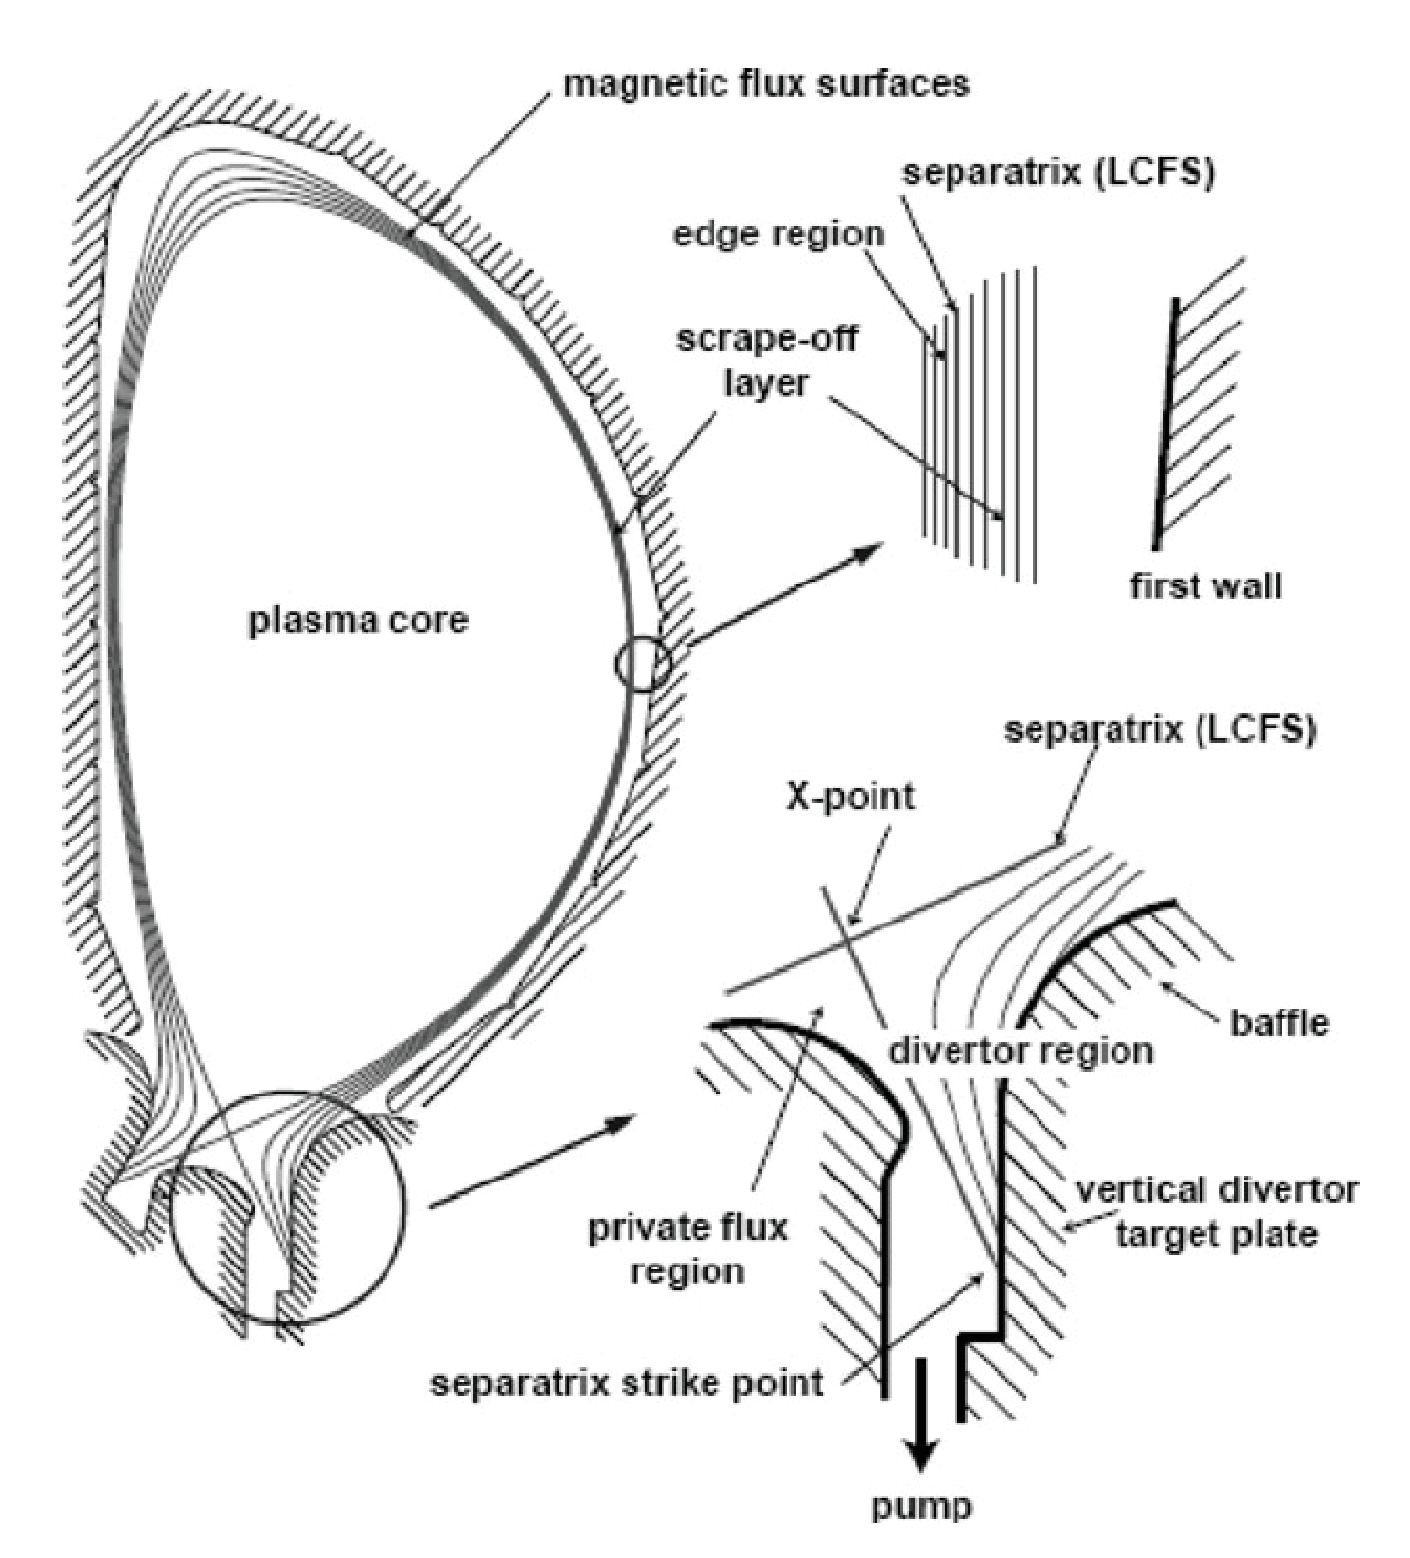
\includegraphics[scale = 0.35]{graphics/edge_anatomy.eps}
  \caption{The taxonomy of terms used to describe the edge are shown for the case of a divertor tokamak configuration; limiter terminology follows similarly. External coils combined with the toroidally driven plasma current produce a helical magnetic field that traces out closed flux surfaces. This region of closed field lines constitute the core of a magnetic confinement device. A (poloidal) divertor is shown here that diverts the poloidal field so that a magnetic X-point appears on poloidally projected plane (shown). The magnetic surface that contains the X-point is the \emph{separatrix}, and the region outboard of this surface is the \emph{edge}. Reprinted under free-use policy from the IAEA \cite{IAEA}.}
  \label{fig:edge_anatomy}
\end{figure}

Among the features that characterize the edge is the presence of steep gradients in the density and temperature profiles which constitute what is known as the \emph{pedestal}, the height of which is seen to provide a gauge for the quality of plasma confinement (Figure \ref{fig:pedestal_traces}) \cite{Zohm}. While the mechanisms are not well understood, consistent correlations are seen to exist between power flux through the last closed flux surface and the spontaneous transition from a mode of low (L) to high (H) confinement \cite[p. 4]{Zohm}, a regime marked by an approximate two-fold increase in energy confinement time $\tau_E$ \cite[p. 358]{Stangeby}

\begin{figure}[h!]
  \centering
    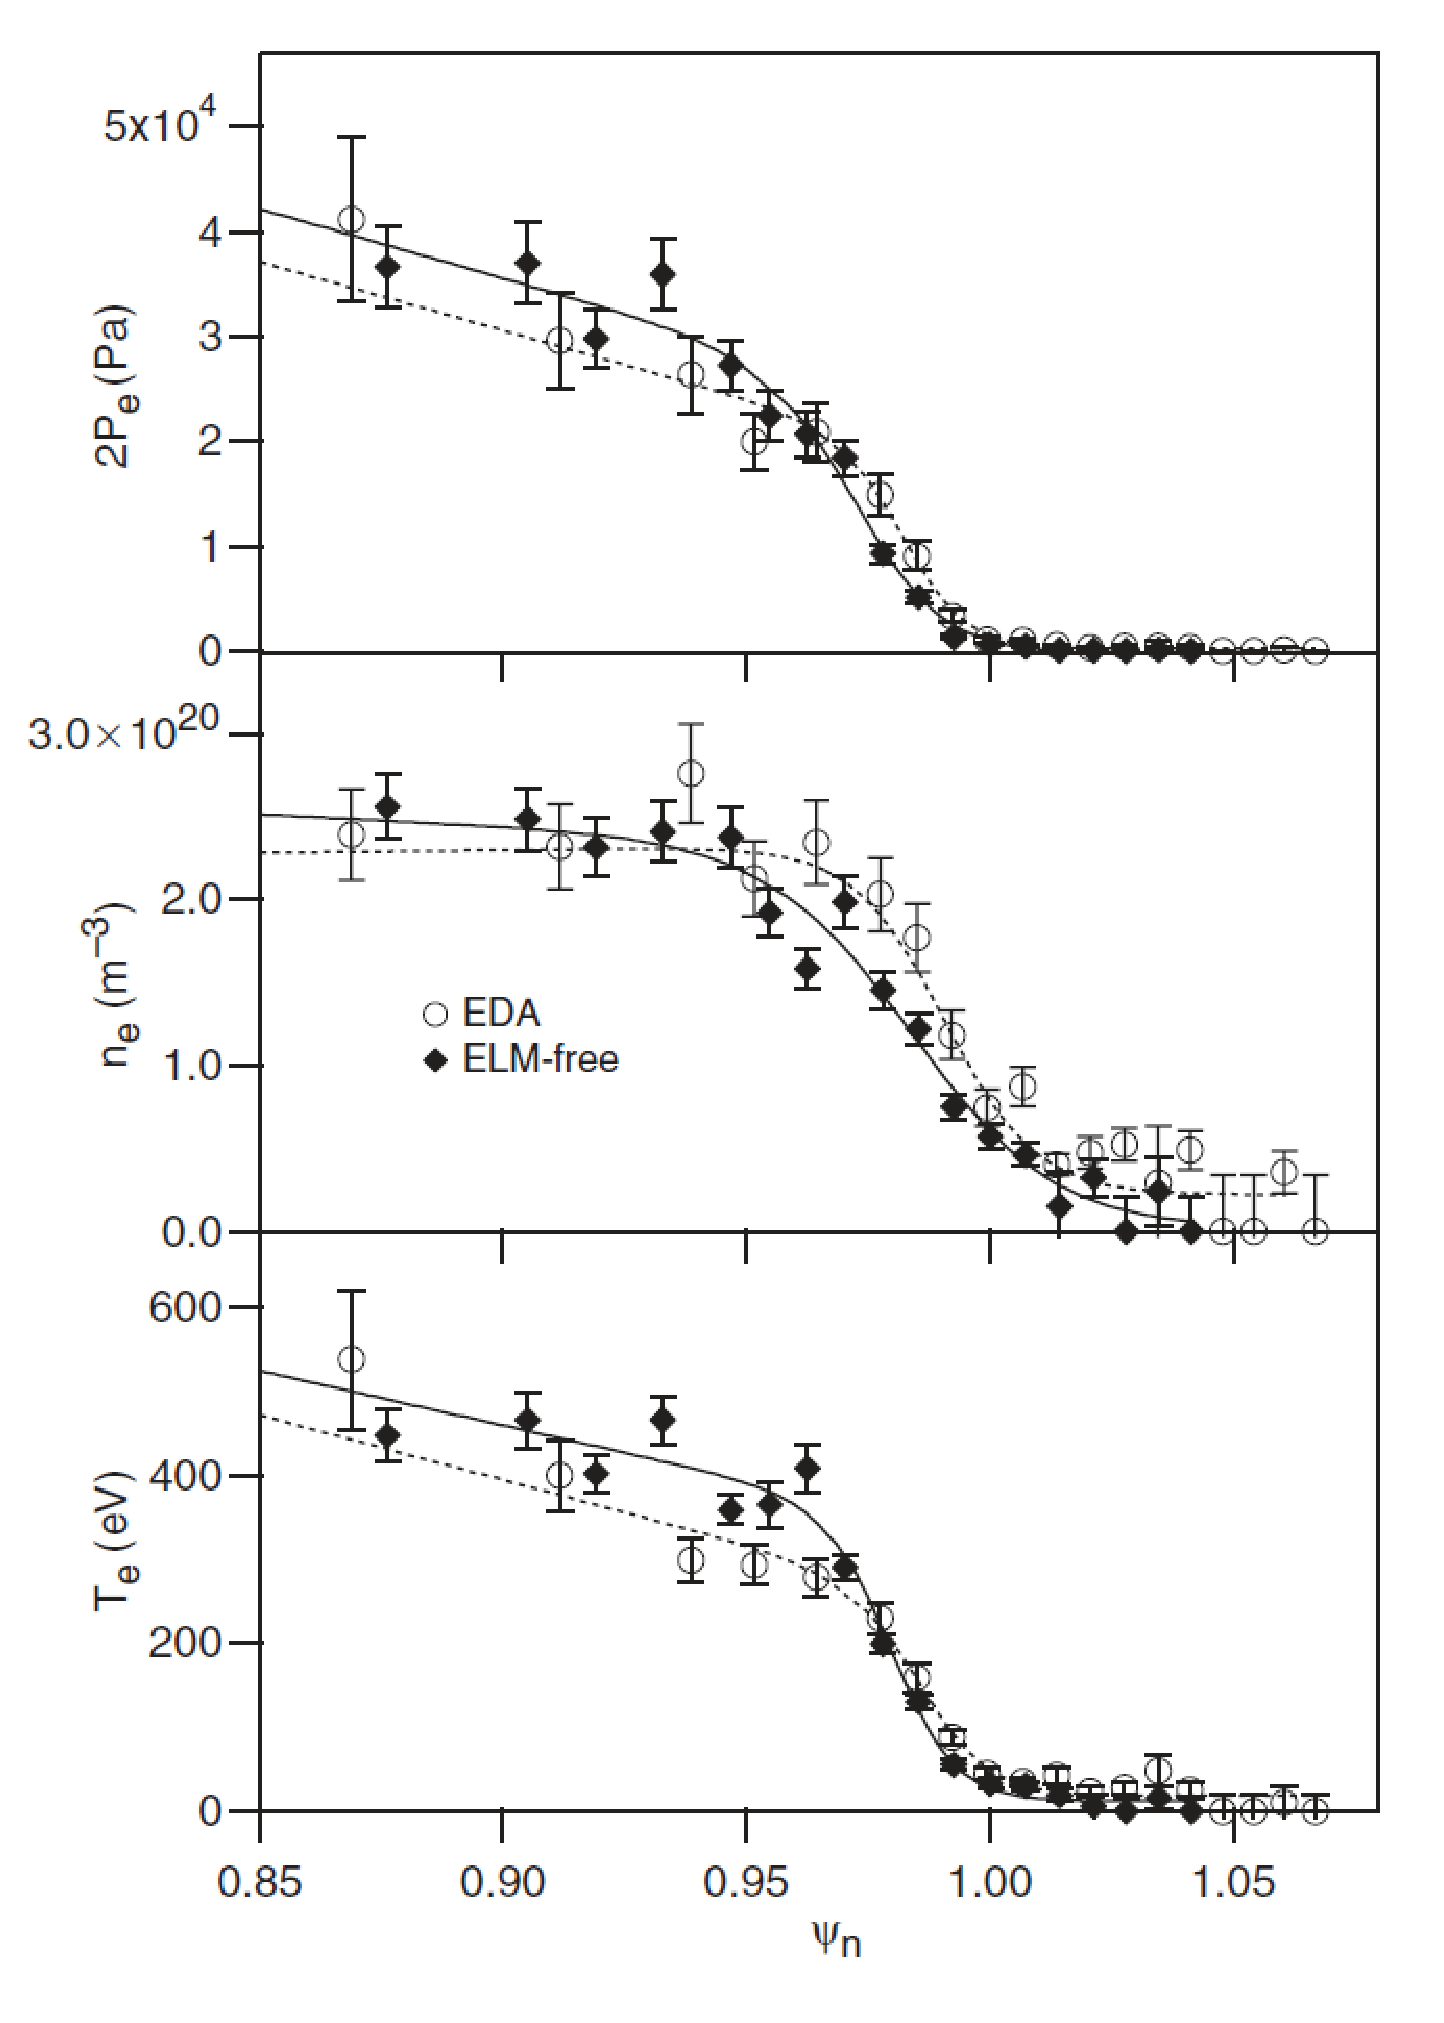
\includegraphics[scale = 0.35]{graphics/pedestal_traces.eps}
  \caption{Typical profiles in the edge region. The sharp gradients in plasma parameters (electron pressure $P_e$, temperature $T_e$, and electron density $n_e$) form an abrupt step in the traces with respect to distance (normalized poloidal flux label $\psi_n$) towards the edge known as the \emph{pedestal}. Here, an experiment on Alcator C-Mod demonstrates two kinds of H-modes: enhanced $D_{\alpha}$ (EDA) mode, and an ELM-free mode \cite{Mossessian02}.}
  \label{fig:pedestal_traces}
\end{figure}

The pedestal is formed due to conditions resulting from the presence of a material boundary and because the charged particles are characterized by a distribution of velocities. In the transition to a high mode (H-mode) of confinement (section \ref{subsec:Unique_physics_in_the_edge}), an internal transport barrier must develop that further amplifies the difference of scales between the core and the more sparse edge region. Notwithstanding, the transition layer occurs even in unconfined systems as Bohm \cite{Bohm} demonstrated without the context of fusion in mind. 

Bohm showed the presence of a material boundary (wall) sets up simple electrodynamical interplay between the highly mobile (less massive) electrons and the less mobile (higher mass) positive ions. The narrative is explained simply as the presence of a the wall constitutes a sink for the mobile electrons which foremostly charge it negative. The negative potential from the accumulation of charge decreases the electron current to the wall by raising the energetic bar required to reach it. Meanwhile, any positive ions in sufficient vicinity are accelerated by the negative wall potential in accordance with the Debye shielding effect which increases positive ion effluxes towards it. The transport is enhanced by the parallel pressure gradient. For ions, the accelerating potential and the pressure gradient encourage ions to flow to the walls, whereas for electrons the electric field set up inhibits incoming fluxes though its parallel pressure gradient notwithstanding helps it (figure \ref{fig:Stangeby_1Dplasma_params_edge}). 


\begin{figure}[h!]
  \centering
    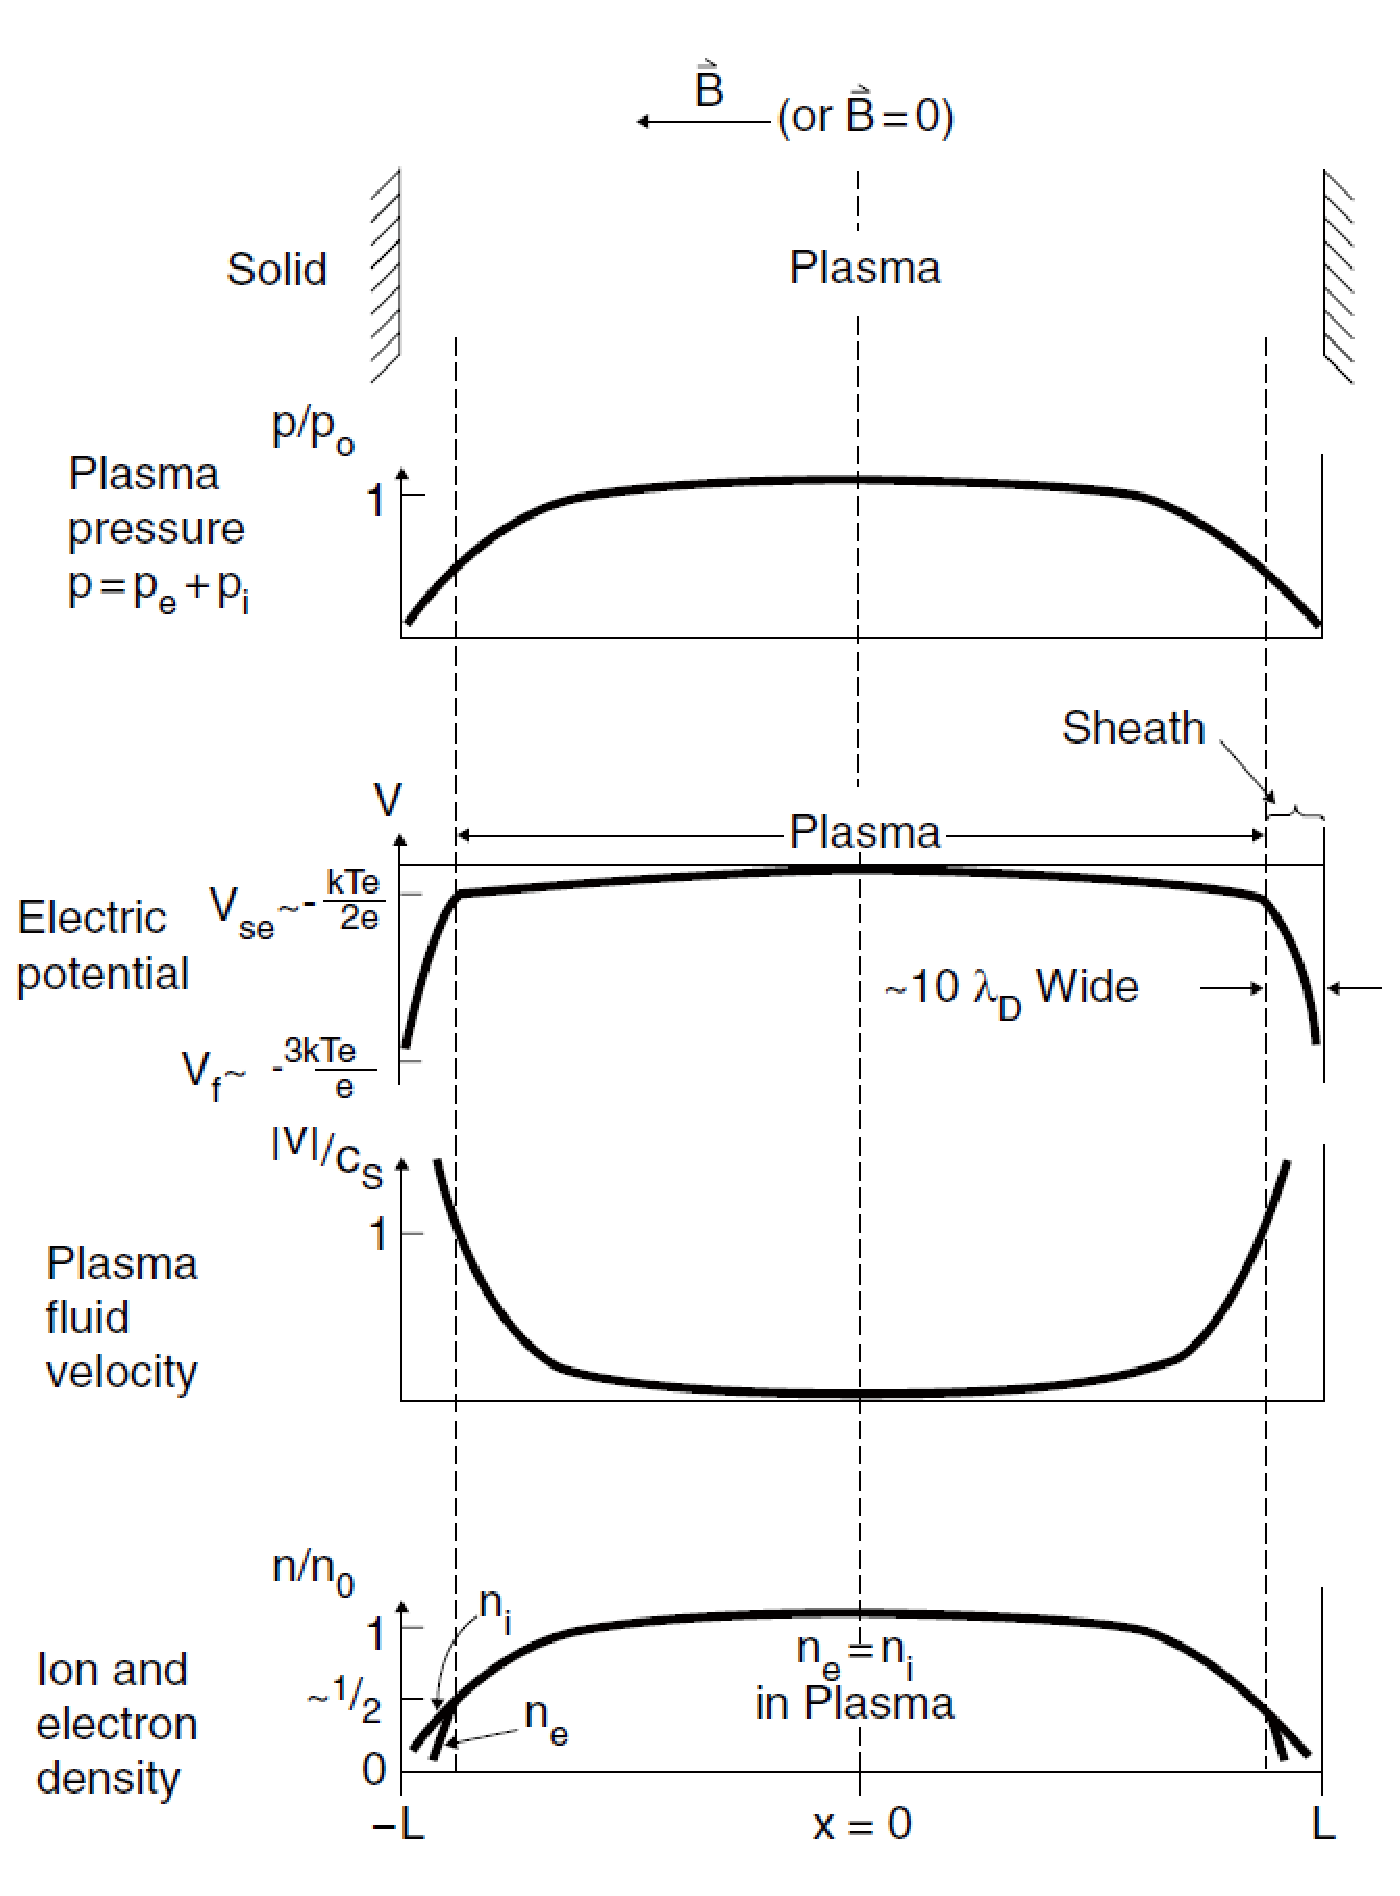
\includegraphics[width=0.5\textwidth]{graphics/Stangeby_1Dplasma_params_edge}
  \caption{Traces of plasma parameters when walls are present}
  \label{fig:Stangeby_1Dplasma_params_edge}
\end{figure}

The ion current makes the potential at the wall less negative; however, this simultaneously permits a larger range of electrons to reach the wall which lends itself to make the potential more negative. The two competing processes interplay until an equilibrium is reached, marked by the condition of equal \emph{fluxes}, known as \emph{ambipolar} flow, which creates a region of positive space charge near the wall known as the \emph{sheath} ($n_i > n_e$, figure \ref{fig:Stangeby_1Dplasma_params_edge}). 

By seeking the potential profile $\phi (x)$ for cold ions ($T_i = 0$) in a fluid plasma as a solution to Poisson's equation ($\varepsilon_0\partial_{x}^2\phi (x) = -\rho(x)$) and matching the solutions obtained from the multiple scales analysis (one solution is obtained for the region pertaining to the core extending to the edge, and the other is analyzed from the edge reaching inward to the core side), Bohm showed that only physical (non-oscillatory) potentials were possible if the monoenergetic ions were accelerated exactly to the sound speed $c_s$ near the plasma wall. This sharp step up in the velocity profile for ions in space defines a clear \emph{sheath edge}. The generalization to a physical plasma which is characterized not by a monoenergetic source of ions, but rather by a distribution results in a smoothing of this sheath edge so that this transition layer is known as the \emph{pedestal} (figure \ref{fig:pedestal_and_poloidal_xsec}).

\begin{figure}[h!]
  \centering
    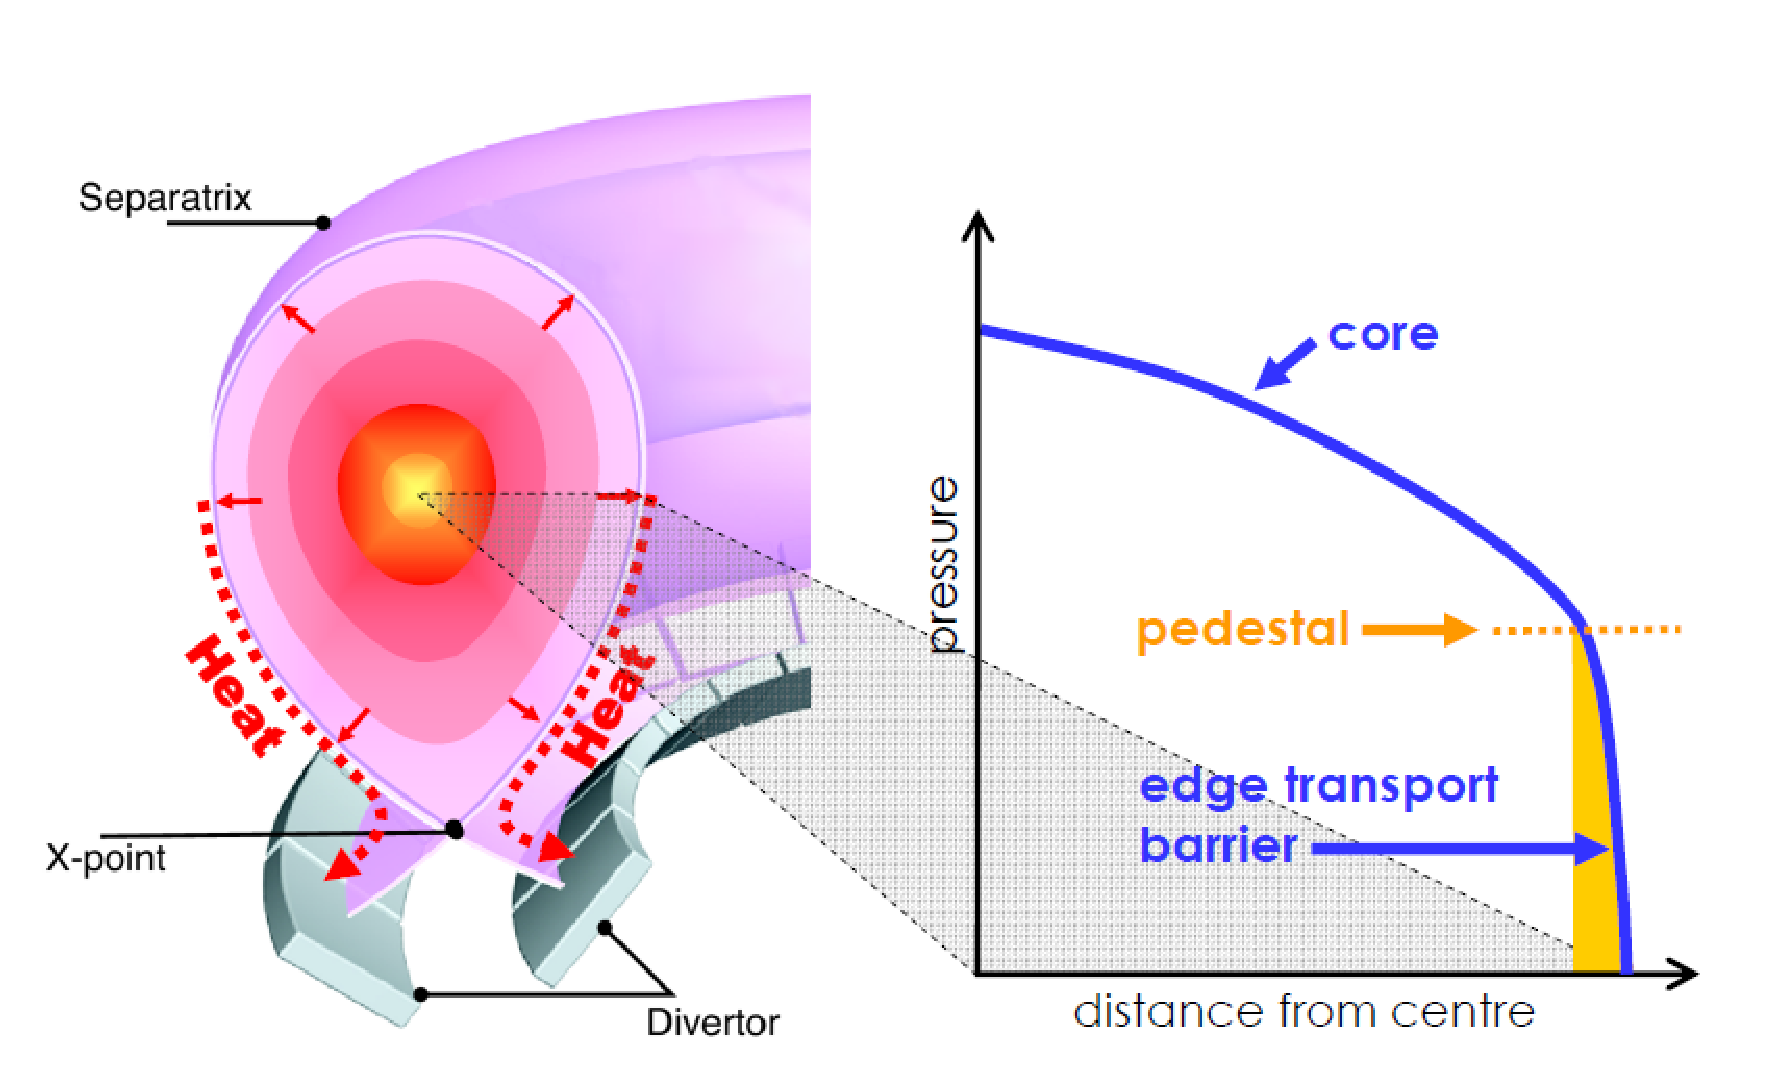
\includegraphics[width=0.75\textwidth]{graphics/pedestal_and_poloidal_xsec}
  \caption{A poloidal cross-section of the magnetic configuration is shown on the left, whereas the plasma pressure along a radial arm from the core center to the edge is shown where the pedestal is identified in comparison with the core and edge \cite{ConnorXX}.}
  \label{fig:pedestal_and_poloidal_xsec}
\end{figure}


Properly, the Bohm criterion refers to one side of the inequality from the aforementioned multiple scales stepthrough. It expresses that ions from the core are accelerated to at least the sound speed $c_s$ at the sheath edge ($se$) when ``exiting'' the plasma to reach the material boundary:

\begin{equation}
v_{se} \geq c_s , \qquad \qquad \qquad \text{\underline{Bohm criterion ($T_i = 0$)}\label{eq:Bohm_criterion_fluid}}
\end{equation}

\noindent Thus, the Bohm criterion sets a lower bound of the ion exit velocity \cite{Stangeby}. The requirement obtained when considering the problem from the core-side enforced that $v_{se} \leq c_s$, so that the equality is converged on when the two solutions are matched. The generalization to $T_i \neq 0$ produces a similar, yet distinct condition:

\begin{equation}
\int_0^{\infty} \frac{f_{se}^i(v) dv}{v^2} \leq \frac{m_i}{kT_e} , \qquad \text{\underline{Bohm criterion ($T_i \neq 0$)}\label{eq:Bohm_criterion_kinetic}}
\end{equation}

\noindent where $f_{se}^i$ is the distribution function for the ions at the sheath edge ($x = x_{se}$). Thus, the edge region in a magnetic confinement device is characterized by the the region of open field lines that extends outboard to the material boundary where invariably we encounter \emph{sheath physics} whose sheath thickness is dictated by details contained only in a kinetic description.




\subsection{Unique issues in the edge}\label{subsec:Unique_physics_in_the_edge}

\indent \indent The confinement improvement when operating in H-mode is seen to be \emph{too good} in the sense that the enhanced confinement of the core leads to extreme gradients in the scrape-off layer which ultimately can lead to the generation of unique problems that pervade the edge region \cite{Finken}. Two such problems are edge localized instabilities and the power dilution of the plasma by impurity influxes produced from the plasma interaction with the plasma facing components. Peaked fluctuations (figure \ref{fig:ELM_traces}) in both plasma and field quantities are observed in this region which are regarded as signatures of the microturbulent (anomalous) transport that significantly amplify cross-field outfluxes of particles as compared to neoclassical predictions. Further still, the aforementioned instabilities deliver more high energy fluxe to the material boundary. The repeated stresses on the materials are not a concern for present day devices; however, the power will be sufficiently higher for larger devices such as ITER, and these repeated bursts of power effluxes to target plates will likely be a limiting factor for reactor lifetime. In this way, it is understood that an acceptably low plasma temperature at the wall must be maintained in order for the plasma wetted targets (divertor plates or limiters) to preserve their material integrity.

\subsubsection{Multi-faced asymmetric radiation from the edge (MARFEs)}

 \indent \indent  With respect to the concern just outlined above, it is possible to engineer a cushion between the target plates and the core plasma with injected neutral populations through puff valves. This limits the power fluxes to the target materials significantly; however, it has been seen that total \emph{detachment} of the plasma volume in this way encourages the formation of persistent stationary structures due to \emph{multi-faceted (poloidally) asymmetric radiation from the edge} (MARFE), particularly from recycled or injected neutral impurity atoms whose mean free path is large and can significantly penetrate into the plasma. Thus, a high amount of power is diluted from fuel ions and and is released through subsequent radiation. This presents a risk in that the plasma suffering a global disruption due to thermal collapse. In tokamaks, these structures manifest as toroidally symmetric aggregates of high density cold plasma at the inboard side of the last closed flux surface. In this way, temperature and density gradient driven transport that are enhanced by the presence of MARFEs will rapidly lead to global disruptions whenever a density limit is exceeded (Greenwald or Murakami limit for tokamaks, or the Sudo limit in stellarators). At densities approaching such a limit, the impurity radiation power is proportional to the square of its density so that it increases until the impurity radiation power becomes equal with the power input. Above this limit the plasma suffers thermal collapse by a corresponding decrease in temperature, thereby increasing resistivity which causes the current to be quenched. Thus, a compromise between the extent of detachment and power fluxes to plasma wetted targets must be settled on so that heat loads to the plasma facing components (PFCs) can be reduced while simultaneously discouraging the formation of these radiation precipitates. The recommendation for ITER is to operate in the \emph{partially detached regime} wherein the inner divertor plate is completely detached, but the outer plate is only partially shielded \cite{EFDA_MARFE}. In this way, the detached regions correspond to plasma particles whose connection length is longest and whose strike point is most remote from the plasma core. Impurity atoms from the recycling process will then not penetrate too far into the SOL in order to stave off disruption events of this kind.

% The plasma surface interaction realized at either divertor target plates or limiters demands careful management of neutral particle and plasma recycling.
%   [Note to self: cf. p.494 of Stangeby for discussion on how to achieve detachment -- require a balance of particle, momentum, and power. Cannot power starve a plasma into detaching given coupling to the other two conservation equations).

\subsubsection{Edge localized modes (ELMs)}

\indent\indent A unique collective phenomenon that occurs in edge of H-mode plasmas are the so-called \emph{edge localized modes} (ELMs). Such wave phenomena occur with regular periodicity whose appearance and quenching show provisional dependence on the power flux through the last closed flux surface (LCFS) in limiter systems, or equivalently the separatrix in divertor configurations. ELMs present with periodic tone bursts of directed plasma density in certain regimes that can deleteriously bombard the plasma facing components with high power fluxes. Further, the presence of ELMs is known to decreases the extent of confinement as shown generically in figure \ref{fig:ELM_effecT_on_confinement}.

\begin{figure}[h!]
  \centering
    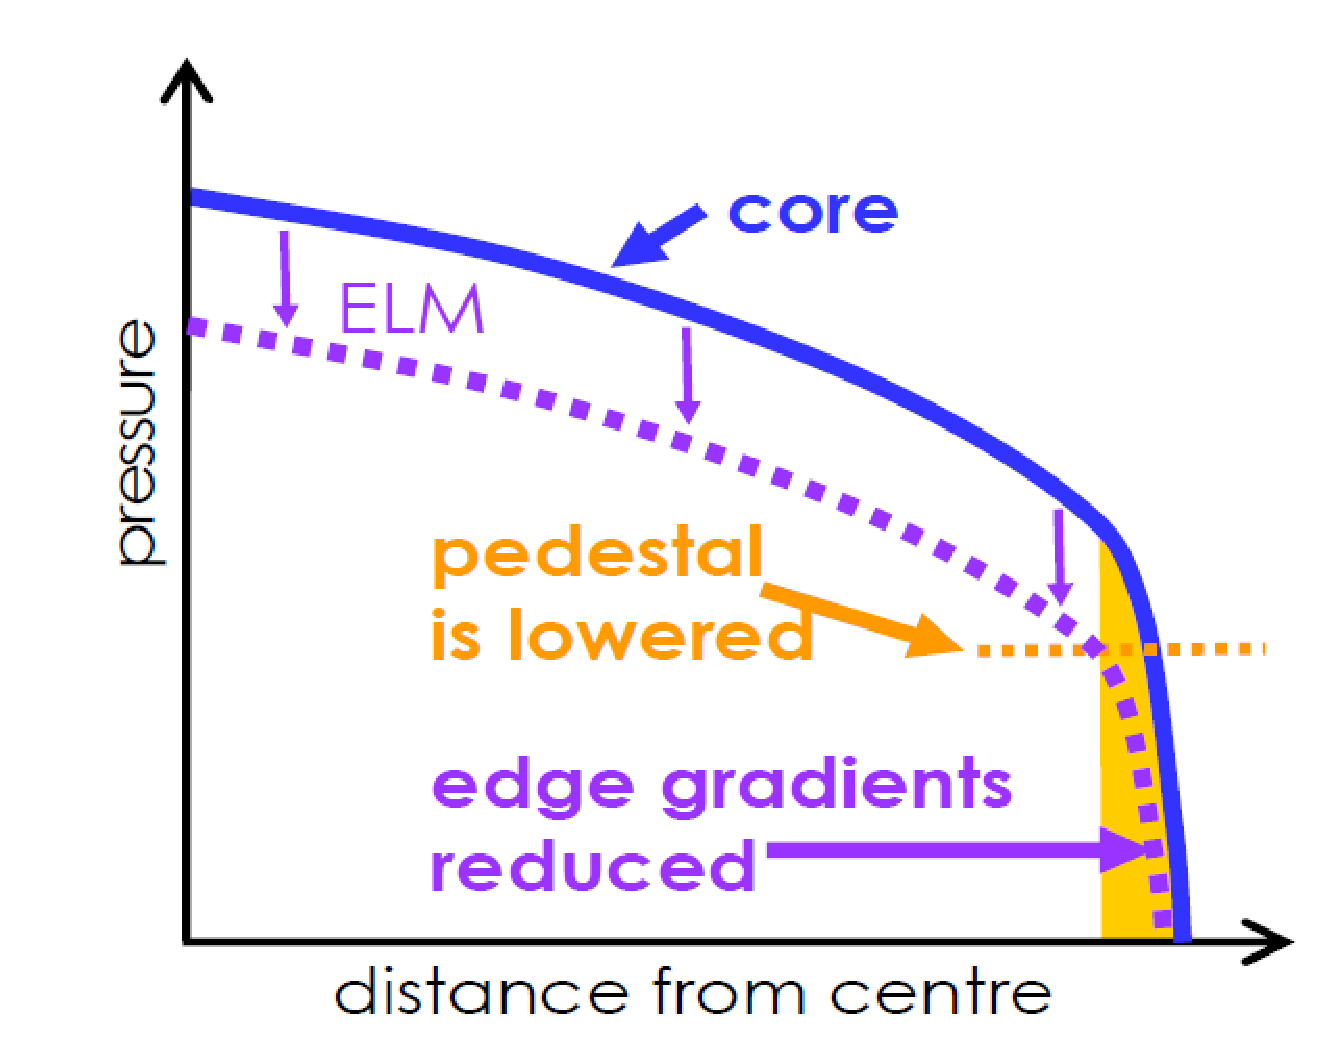
\includegraphics[width=0.45\textwidth]{graphics/ELM_effect_on_confinement}
  \caption{When an ELM removes density from the edge region, the edge gradients decrease and so does the pedestal which directly reduces the confinement of the core \cite{ConnorXX}.}
  \label{fig:ELM_effecT_on_confinement}
\end{figure}

\noindent Notwithstanding, the elimination of ELMs is not desirable as it has utility in sweeping helium ash and impurites out of the plasma that would otherwise accumulate without a means to remove it. ITER intends to operate in a so-called \emph{ELMy H-mode}. 

Since ELMs are within the scope of the engineering of a fusion reactor design, we first note briefly the means by which their presence is dealt with or otherwise handled. While occassional ELMs are desired, their manifestation must be managed or minimized. Designs incorporating an ergodized edge and/or using error field correction coils (EFCC) have demonstrated the plasma effluxes can be distributed and ELMs can be mitigated \cite{Nardon}. Ergodicity in the edge region is accomplished by external coils that induce resonant magnetic perturbations with respect to $q$ rational. We define \emph{ergodicity} to mean introduced radial excursions of a field-line in its otherwise helical pathway as compared to the confined core. The result is enhanced radial transport in the presence of already strong parallel transport. Such confluent flows flatten the temperature profile with the aim of increasing the area of particle fluxes on the target plates to make the power deposition on the PFCs more reasonable. Combining an ergodic edge with an injection of an impurity (neon or argon are most common) also assists to reduce the power loads as the chaotic region of magnetic field lines spreads the exiting particles over a larger three-dimensional volume so that the chance of momentum exchange with impurity ions is more likely. In doing so, a radiation mantle can form with respect to the divertor plates and the resulting charged particle fluxes to the PFCs is reduced further.  Lastly, more targeted stochastization of the edge magnetic field using resonant magnetic perturbations (RMPs) has also proven viable for active ELM control in devices such as KSTAR \cite{EFDA_KSTAR_ELM_control}, and most recently by DIII-D with ITER-like shaping and collisionality \cite{DIII-D_ELM_suppression}; JET has been in the process of updating its system to accommodate an RMP attachment. 

\subsubsection{Types of ELMs and regimes of operation}

\indent\indent Edge localized modes are categorized by an enumerated type (I, II, and III), whose existence show clear delineations with respect to power flows through the LCFS. While the dependence is observed on the power through this flux surface, ELMs are classified most usually in terms of power input given it is a directly controlled experimental parameter. A general feature of these instabilities are their repetitiveness; ELMs appear as disturbances of the H-mode plasma periphery whose periodic relaxation mechanism results in pulses of directed high energy density plasma towards the walls of the confinement device. It is thought that ELMs originate as MHD instability (peeling-ballooning mode) caused by gradients in either pressure or current. Below, we step through each type in the order they are encountered for increasing values of the power input. 

\begin{figure}[h!]
  \centering
    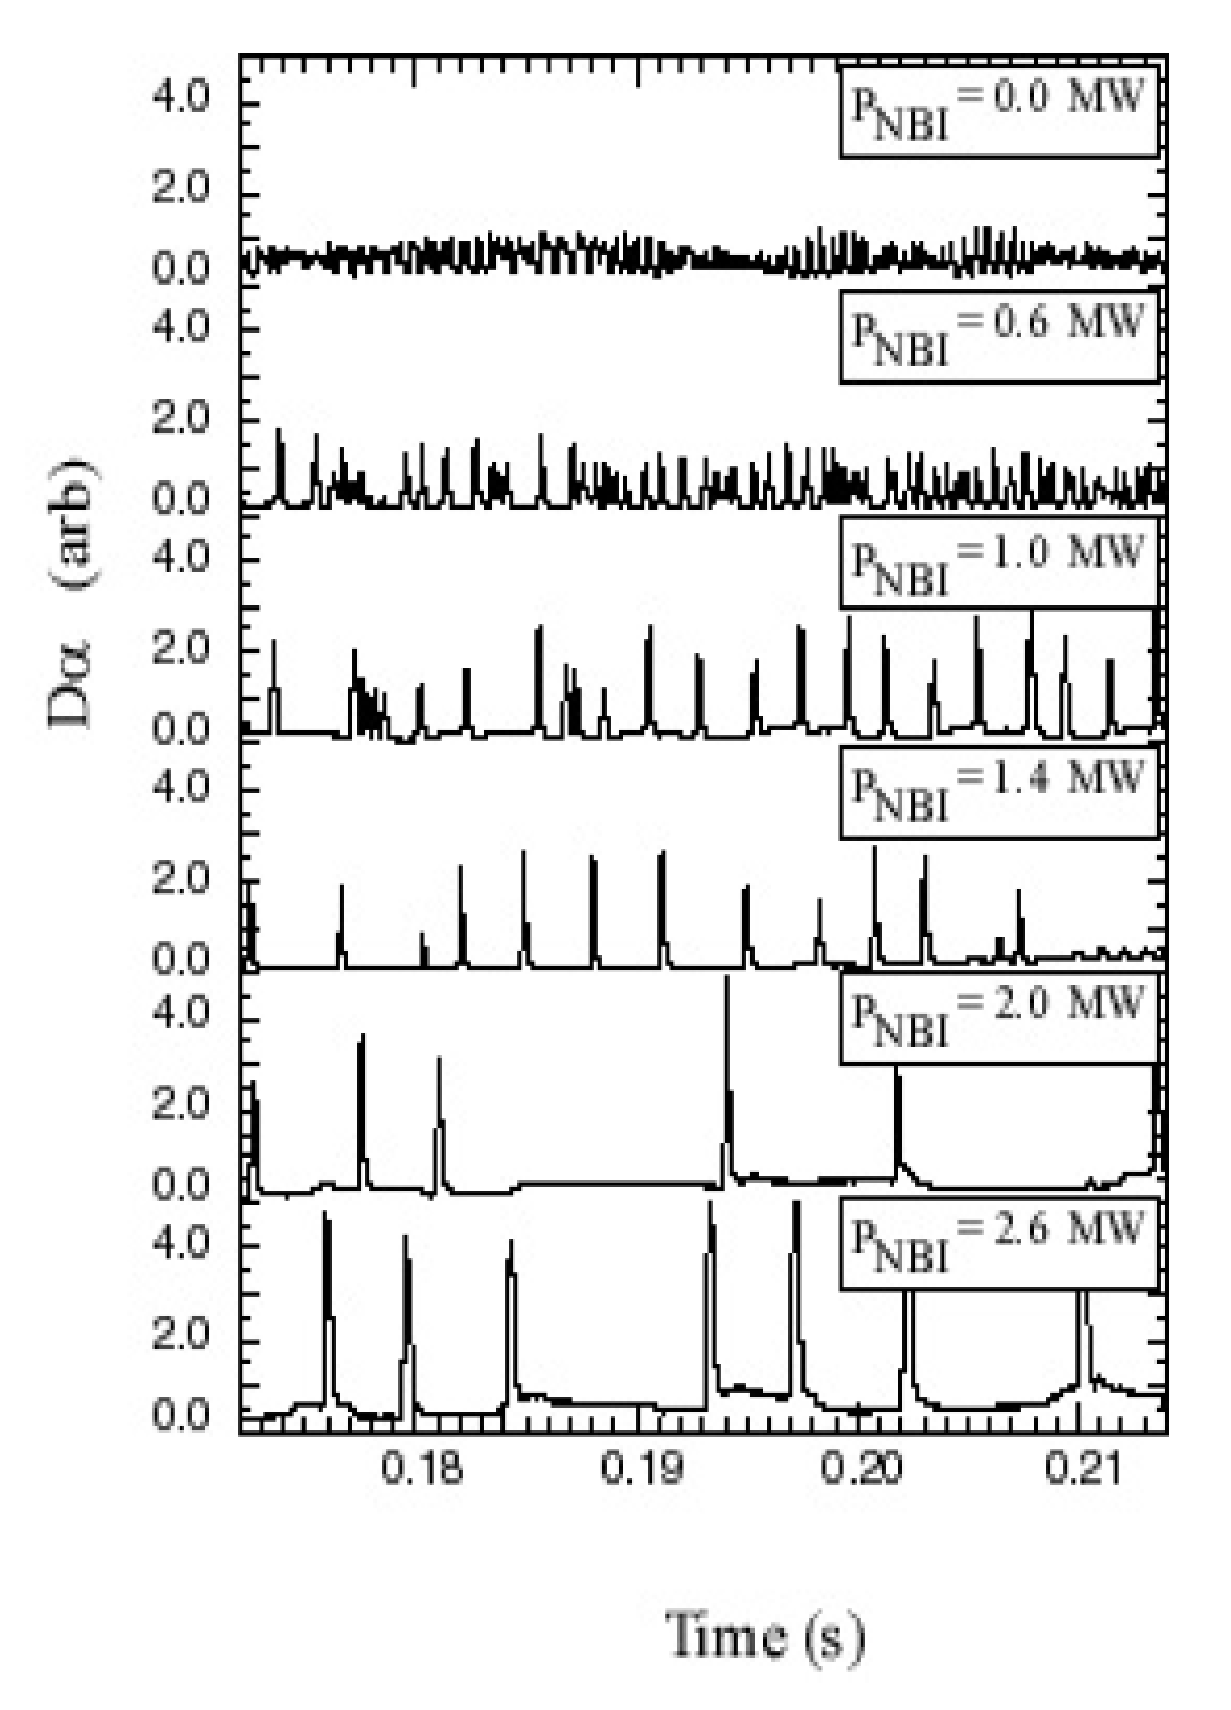
\includegraphics[width=0.45\textwidth]{graphics/ELM_traces}
  \caption{$D_{\alpha}$ measurements for different neutral beam injection (NBI) power inputs $P_{NBI}$. As the power increases, a regularity is achieved that emblemizes type III ELMs. Higher still, the type III ELM is exchanged for the giant type I ELMs shown in the final bottom two plots \cite{ConnorXX}.}
  \label{fig:ELM_traces}
\end{figure}


Type III ELMs develop at the lowest power inputs, decreasing in their frequency of recurrence with increasing power input until they become fully damped. A similar, yet distinct, phenonemon is observed as rapid interchanges between (L and H) modes near the L-H mode threshold power input (the \emph{dithering H-modes}). These events are distinguishable from type III ELMs only insofar as that a high frequency magnetic field fluctuation is observed in the edge for type III ELMs as a precursor to its onset; this marker is absent in the dithering between modes. As the power input is increased further an intermediate range is reached, devices with highly shaped plasmas (triangulation and elongation) have witnessed generation of type II (\emph{grassy}) ELMs whose repetition frequency ostensibly show no significant dependence on power input. As the power is increased higher still, type II ELMs are traded for type I, or \emph{giant}, ELMs whose frequency is seen to increase with power (figure \ref{fig:ELM_traces}). Since the grassy (type II) ELMs are observed only in highly shaped plasmas, it is inviting to consider designing less shaped systems that then will exhibit quiescent regimes for intermediate power input. Thus, it seems possible to operate in an ELM-free regime to minimize damaging power loads to the plasma facing components (\emph{QH modes}). This had first been achieved at DIII-D by counter-injection of neutral beams (against plasma current) alongside cryopumping for density management \cite{Burrell02, Burrell09}, but has since been shown to be attainable with either co- or counter-injection with respect to the sign of edge rotation so long as the magnetic shear in this region is sufficiently high \cite{Burrell01, Burrell09}. QH modes had later been demonstrated in tokamak experiments such as JT-60U and the ASDEX-Upgrade \cite{Suttrop04}, as well as NSTX \cite{Park}. The disadvantage to such modes originally was outpumping of impurity densities at the edge without affecting energy transport in the core; however, characteristic edge harmonic oscillations (EHOs) were seen to develop in tandem with the onset of the QH mode which helped remove impurity buildup naturally as the EHOs enhance edge transport which permits outpumping of impurity accumulations as needed without affecting the core confinement. It has been suggested that this regime likely can maintain acceptable energy confinement times at the requisite densities \cite{Loarte03}. Like ELMs, EHOs suggest their mechanism lies in MHD. However, they are seen to occur in an operating space below the peeling-ballooning instability limit. 

It is alternatively seen that one may forego the aforementioned concern in favor of operating at higher power inputs by highly shaping the plasma. It has been demonstrated for multiple devices that while highly shaped plasmas exhibit grassy ELMs at intermediate power, type I ELMs at higher power inputs are damped out or otherwise evaded at the power injections desired. The role of shaping can be understood as raising the peeling-ballooning mode stability limit on power flow through the separatrix (or LCFS) so that systems can be designed to operate at higher desired power injections but still below type I ELM range. To this end, it is noted that puffing neutral populations to dilute some of the power through impurity radiation in the edge also directly accomplishes the same result \cite{Zohm}.  Pursuant of this pathway allows the so-called \emph{very high} (VH) mode of confinement to be achieved. For example, by modulating the triangularity of the confined plasma, JET was the first device to accomplish this,  which is exemplified by an increase in energy confinement time by a factor of 1.5 above the conventional H-mode in the same device (JET) \cite{Jackson91}. Notwithstanding, the problem of impurity accumulation has precluded goals of the VH-mode of operation in favor of either QH modes with EHOs or ELMy H-mode operation in type I ELM range given both their opportune utility in vacating impurity accumulations. Thus, while the absence of ELMs is seen as a positive with respect to the elimination of pulsed stresses on the plasma facing components, for devices such as ITER the overwhelming recommendation is to operate at a type I ELMy H-mode (although QH investigations are ongoing such as DIII-D and Alcator C-Mod's \emph{enhanced D-alpha} (EDA) mode \cite{ConnorXX}). 



\subsubsection{Additional topics in the edge}

\indent\indent Beyond the local structures that develop in the edge, the crosstalk between the core and the edge plasma is not well understood. Heat and particle transport from the confined plasma into the edge region is not adequately modelled outside of massively parallel multi-physics PIC or gyrokinetic codes (e.g. GENE), as well as within the scrape-off layer itself. To develop the predictive capability needed to understand the heat effluxes bombarding the divertor targets, for example, is a major task of the fusion computation community as the answers to such questions are needed to aid engineering design in the assessment of lifetime of materials. Other topics include the interaction with the wall (recycling of plasma as well as impurity transport back into the core from sputtering off the PFCs). Since the plasma existing in the edge is often non-Maxwellian, full-$f$ kinetic treatments are required which preclude simplifications such as that used by the GENE code which is based on the premise that the distribution function can be linearly superposed as an averaged Maxwellian and a fluctuating component. Such a formulation is not valid in the nonlinear, nonlocal thermodynamic equilibrium region of the edge.

\subsection{Kinetic versus Fluid descriptions}

\indent \indent We are beginning to see the arguments that advocate a kinetic treatment for numerical simulations of plasma systems in the edge region. For example, we note that this generalized Bohm result \eqref{eq:Bohm_criterion_fluid} is inherently a \emph{kinetic} boundary condition that resulted from a fluid model. Thus, in the interest of accurate simulations, the sheath edge can only be properly tracked by computational models that address the kinetic description of plasmas. Further, the presence of a boundary complicates parameter profiles given the physical discontinuity; a detail that cannot be adequately captured by fluid models (figure \ref{fig:Stangeby_edge_distributions}). 

\begin{figure}[h!]
  \centering
    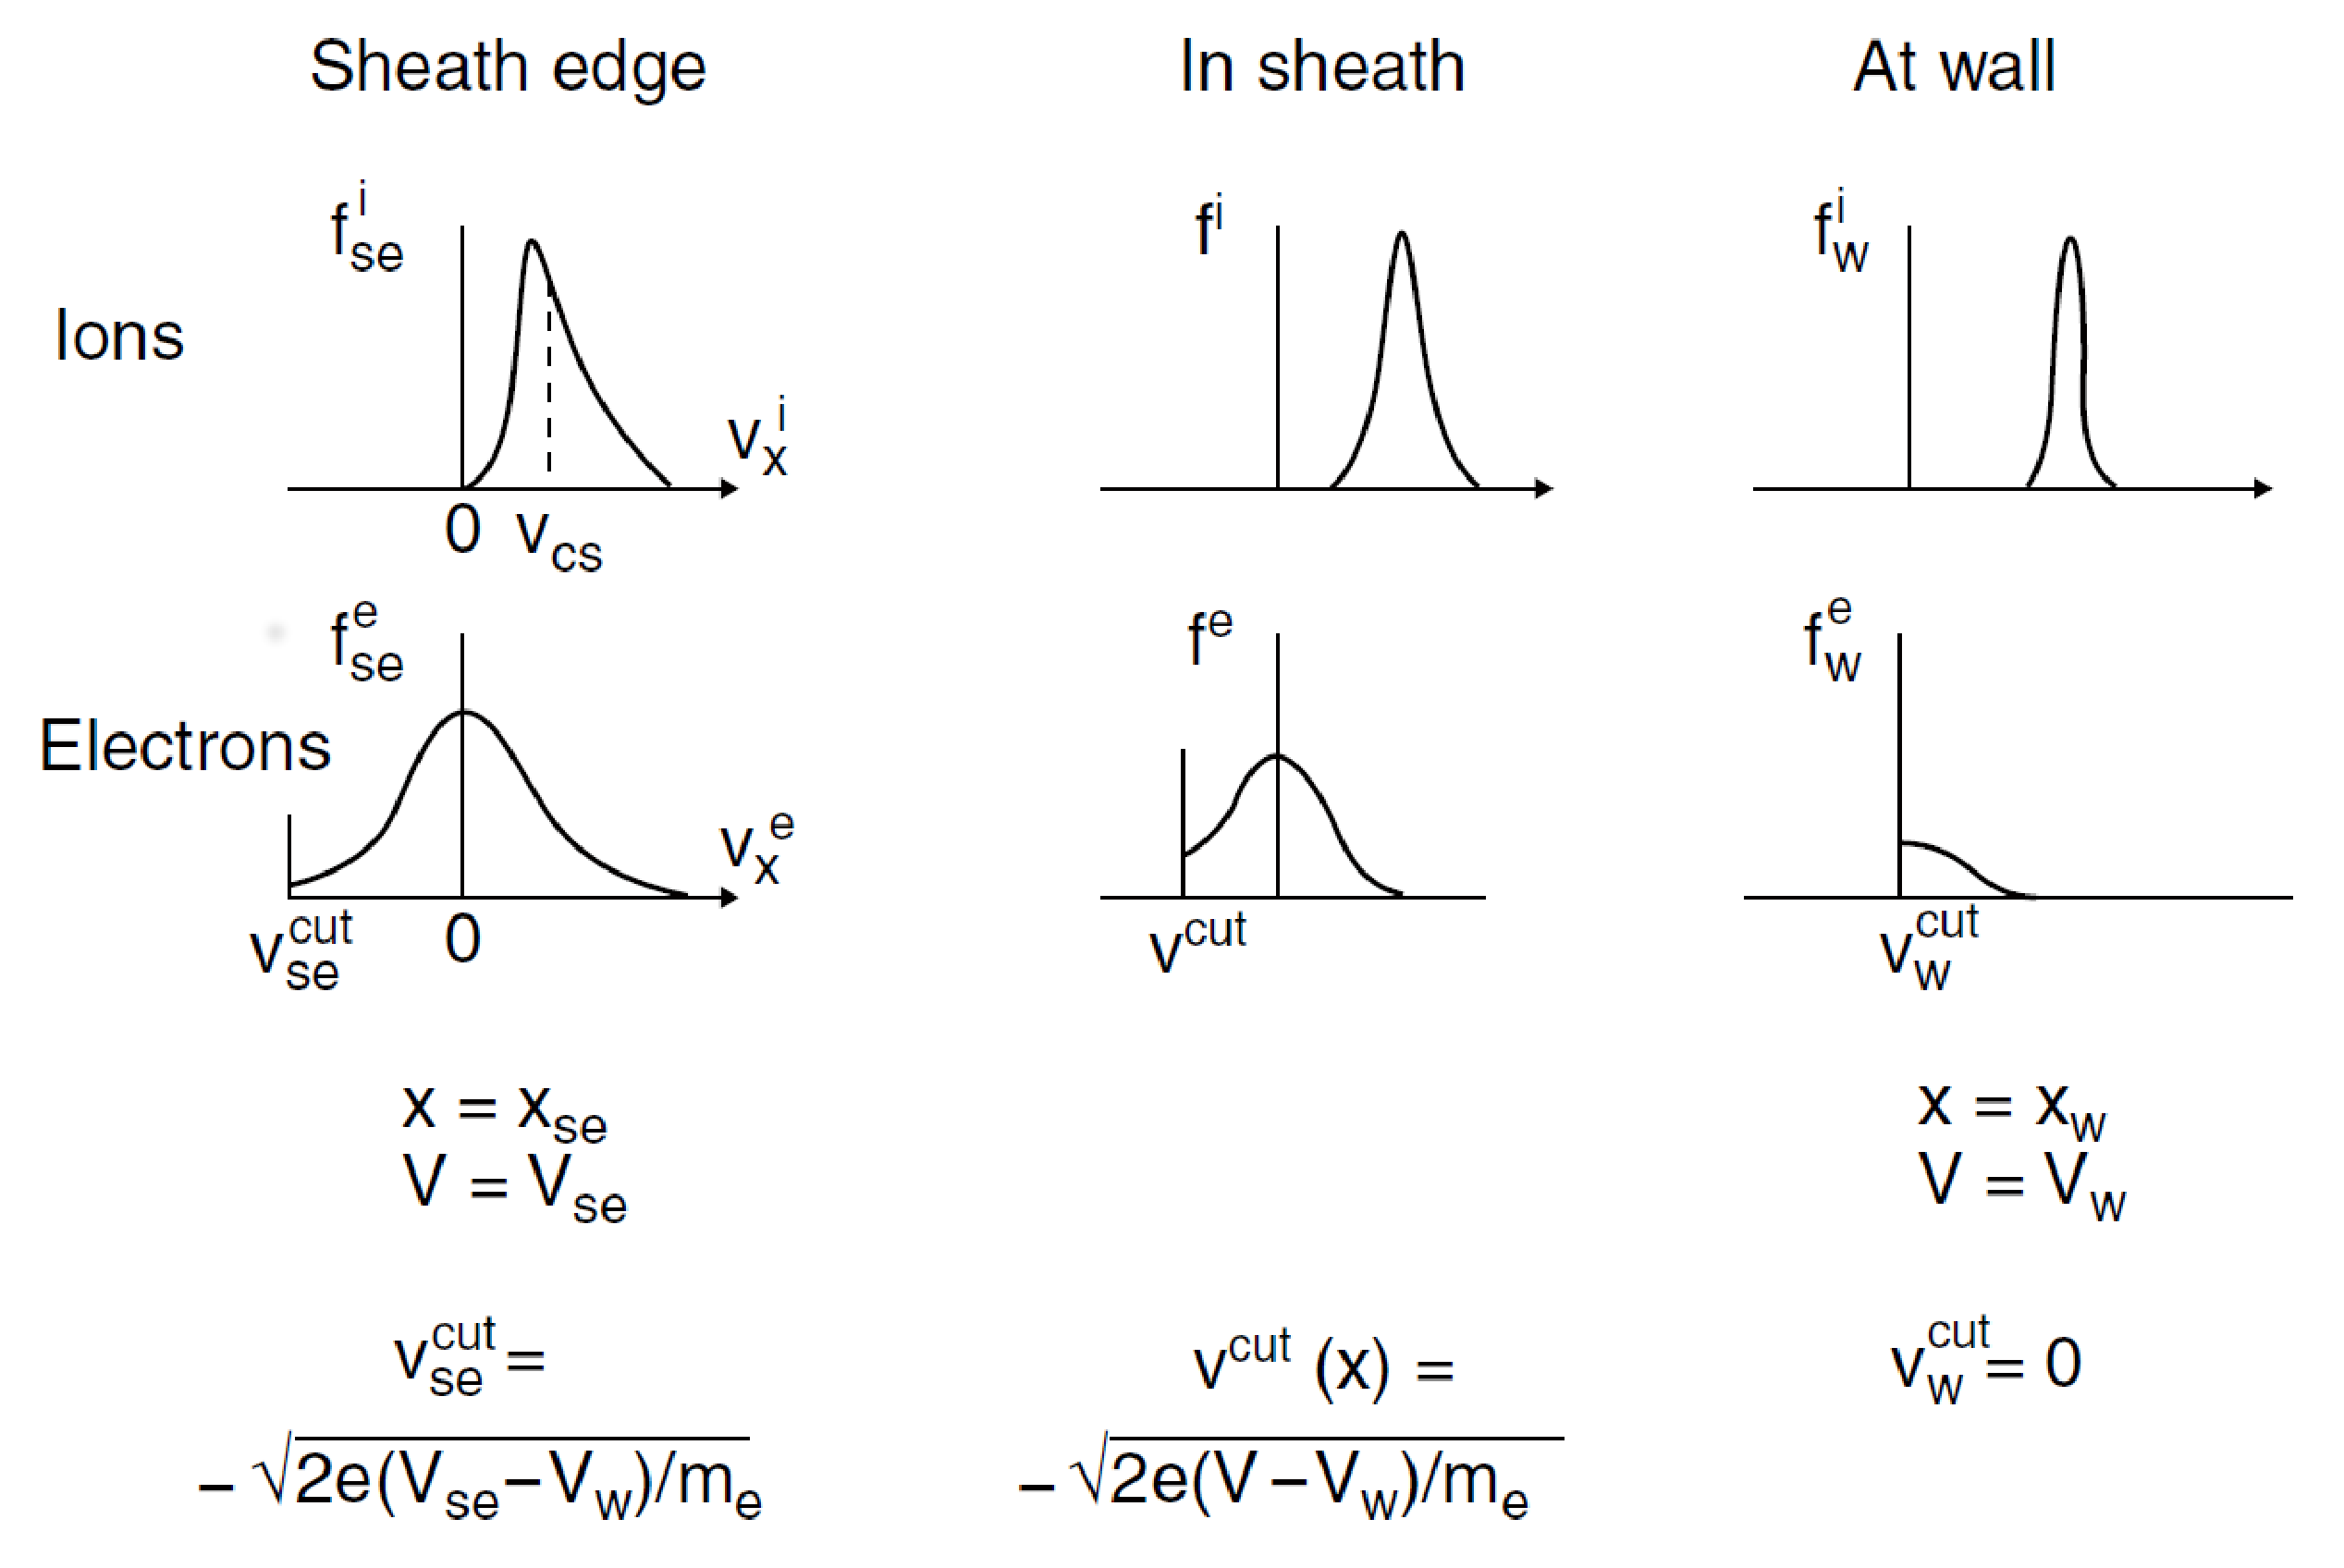
\includegraphics[width=0.75\textwidth]{graphics/Stangeby_edge_distributions}
  \caption{Distributions for the charged particle species at various positions near the wall \cite{Stangeby}}
  \label{fig:Stangeby_edge_distributions}
\end{figure}

Finally, the vastness of scales present in the edge increases the computational burden (figures \ref{fig:SOL_scales}, tables \ref{tbl:tokamak_params_juxtaposition} and \ref{tbl:Stangeby_SOL_scales}). Fluid models cannot capture the physics contained over different velocity regimes (although so-called \emph{kinetic corrections} are applied to capture these effects to some extent). A kinetic treatment is most apt to apprehend these matters directly, especially given the significant role played by the population of charged particles in the high energy tail of the distribution function. Pursuing high order accurate solutions is ultimately constrained by the practical computational cost that can be afforded. As will be argued in a later section, this necessarily motivates methods that have significant finesse so that computational resources can be used as effectively as possible. Thus, a deterministic solution is advocated as more advantageous versus statistical methods given the latter requires simulating large numbers of events in order to capture sparse regions of phase space $(\vec{x},\vec{v})$. The scales span orders of magnitude in densities, lengths, energies, and time scales given the edge region is the transition from the main core to the material boundary. Further, the parameters in the edge can differ significantly depending on one shot to the next, or one \emph{device} to the next. Table \ref{tbl:Stangeby_SOL_scales} juxtaposes edge parameters for the Joint European Torus (JET) and Alcator C-mod at Massachusetts Institute of Technology, which emphasizes the large differences possible. For example, it is commonly argued that high collisionality validates fluid approaches; this table shows in particular that the edge is not necessarily collisional (cf. the normalized collision frequencies $\nu_e^*$ as well as the mean free paths $\lambda_{ee}, \lambda_{ii}$ between the two devices), and that a fluid approach might not capture as much of the required physics as hoped. In consulting this table, we also note the stark difference between these parameters as compared to the core. For example, typical core densities (including those designed for ITER) are an order of magnitude larger ($10^{20} - 10^{21} \, \mathrm{m^{-3}}$) than predicted at the edge ($10^{19} - 10^{20} \, \mathrm{m^{-3}}$), and that the temperatures in the core (keV) are at least three orders of magnitude as compared to those found in the edge (eV). Additional parameters were given for four devices in table \ref{tbl:tokamak_params_juxtaposition}.

\begin{figure}[h!]
  \centering
    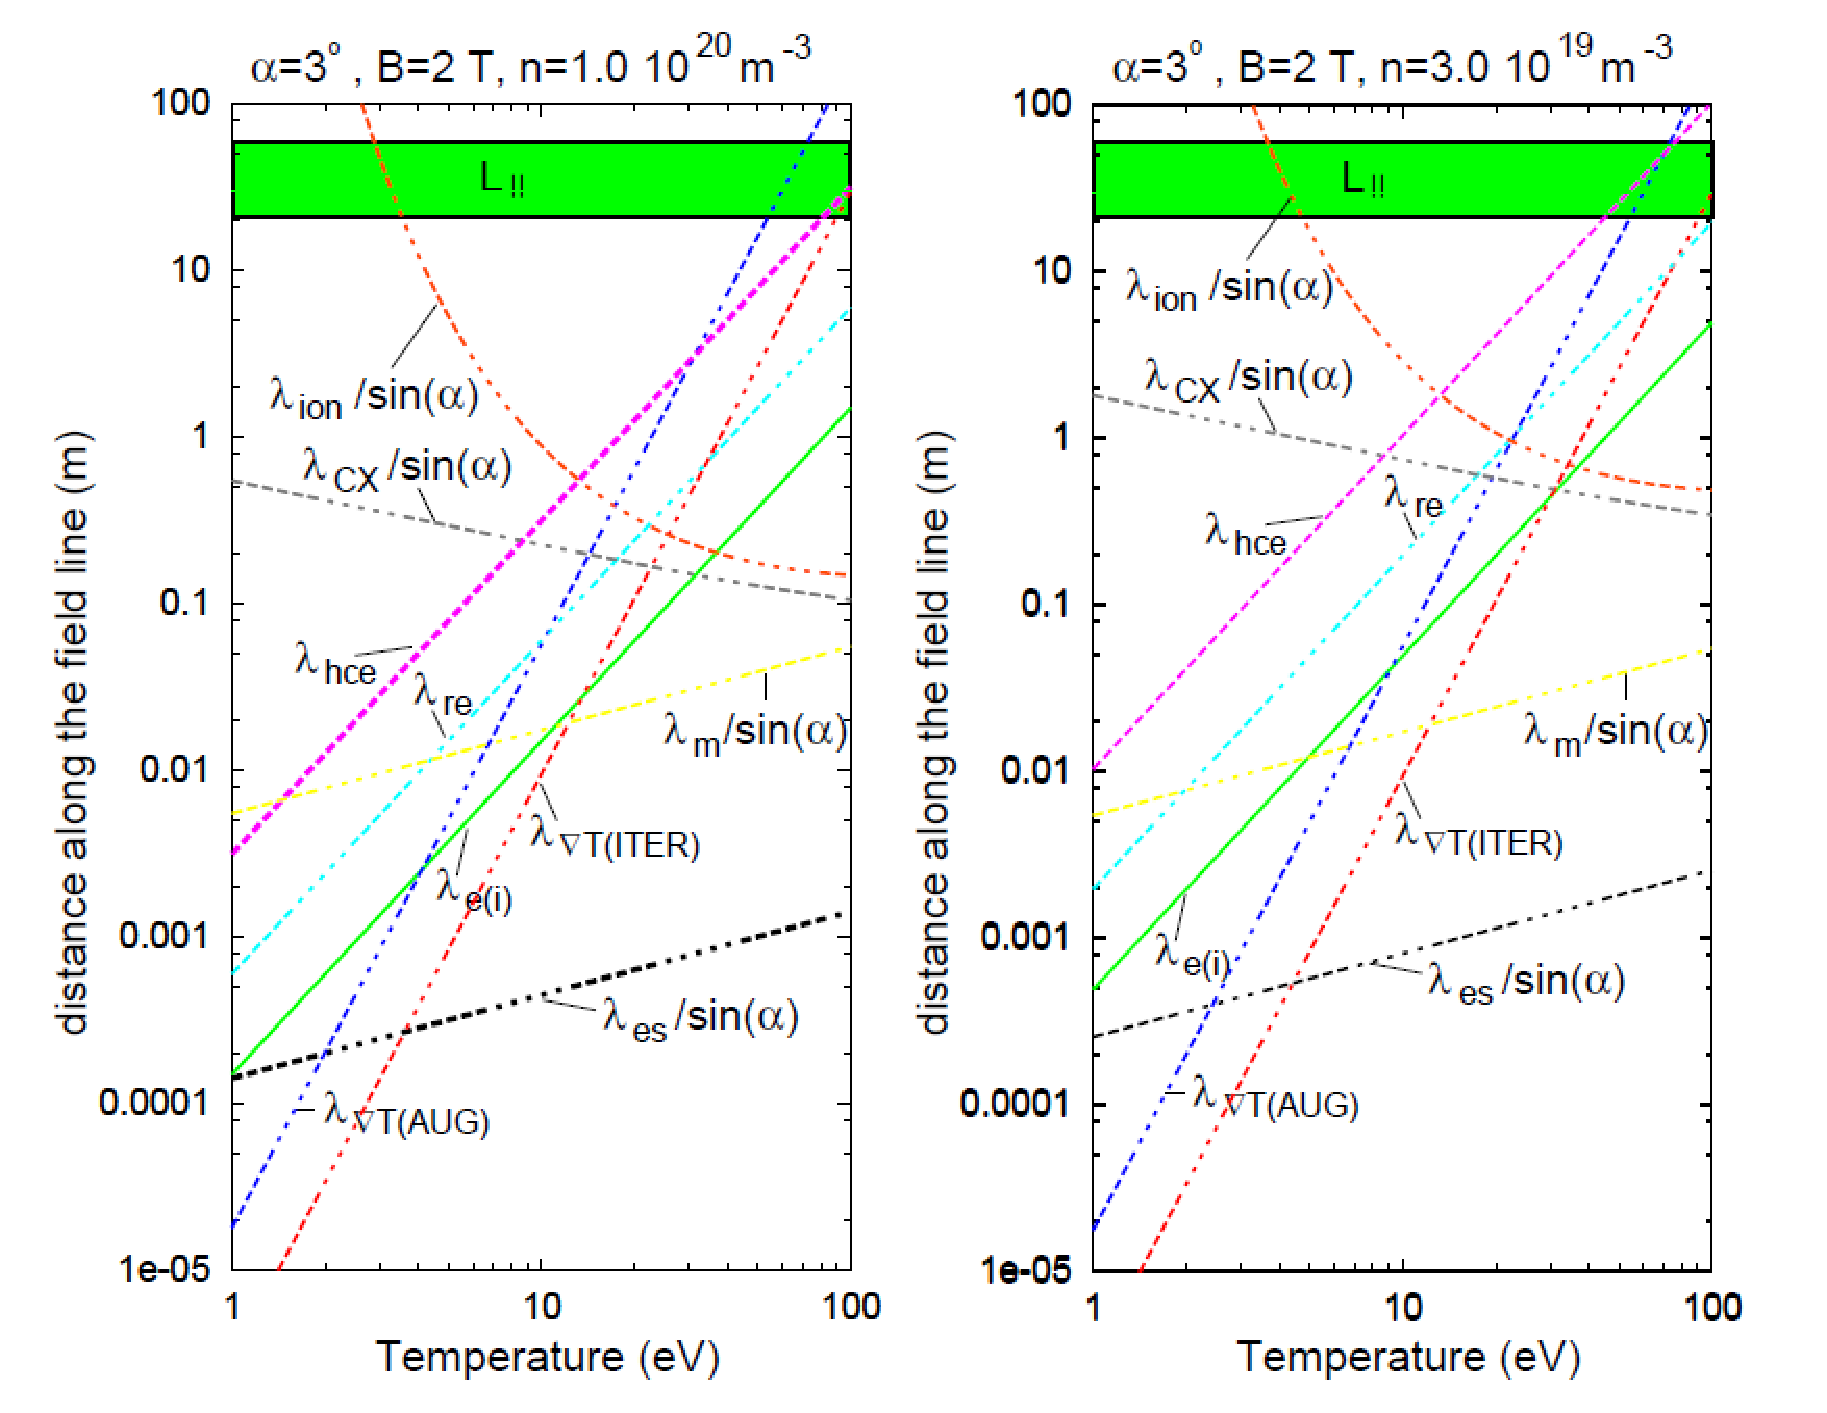
\includegraphics[width=0.8\textwidth]{graphics/SOL_scales.eps}
  \caption{Length scales in the edge for a pitch angle of the $\vec{B}$-field of $\alpha = 3^{\circ}$.}
  \label{fig:SOL_scales}
\end{figure}

\begin{table}\centering
\ra{1.4}
\begin{tabular}{@{}llclclcl@{}}\toprule[2 pt]
&\multicolumn{1}{c}{JET} & \phantom{abc} & \multicolumn{1}{c}{Alcator C-mod} \\
\midrule
\phantom{a}Parameters & &&  \\
\phantom{a}electron density $n_e$ [$\text{m}^{-3}$]	&	$10^{19}$	&&	$10^{20} -10^{21}$       \\
\phantom{a}$T_e$ [eV]	&	50	&&	10 \\
\phantom{a}Connection length $L$ [m]         &	40	        &&	8	\\
\phantom{a}$\nu_e^* = \nu_e / \nu_{e,bounce}$	& 25    	&&	1000	\\
\phantom{a}self-collisional mean free paths $\lambda_{ee}, \lambda_{ii}$ [m]  &	2.5	        &&	0.01	\\
\phantom{a}SOL dwell time $\tau_{SOL} = L / c_s$ [ms]  &	0.6	        &&	0.3	\\
\bottomrule[2 pt]
\end{tabular}
\caption{Parameters in the scrape-off layer (SOL) for two tokamak devices. Reproduced from \cite[p.21]{Stangeby}.}
\label{tbl:Stangeby_SOL_scales}
\end{table}

%Of course, there exists strong anisotropy in the energy exchanges in a plasma parallel and perpendicular to field-lines. In devices such as W7-X, the parallel conduction ($\kappa \sim T_e^{5/2}$) is $10^{4} \sim 10^{7}$ times larger than the cross-field conduction. The parallel transport is predominantly caused by Coulombic interactions, whereas the conduction perpendicular to the field lines is largely turbulent (anomalously) driven, characterized by a diffusive parameter on the order of $\chi_{\perp} \sim 1 \, \mathrm{m^2 / s}$ \cite[p. 15]{Stangeby}. The extent of this anisotropy \ldots

% v_perp ~ 1 m/s whereas v_parallel ~ c_s, p.15 stangeby




\section{Computational methods survey}

\indent \indent In this section we present a brief overview of a selection of alternate schemes applied to the solution of equations in the same family as the Boltzmann-Maxwell set.


%\subsection{Discrete Velocity Model}

\subsection*{Particle-in-cell methods}

\indent \indent Particle-in-cell (PIC) techniques constitute special cases of particle-mesh (PM) methods in that interactions of particles occur through averaged fields on a fixed mesh. The distribution function is discretized into shaped clouds (or macro\emph{particles}) occupying \emph{cells} in phase space that are evolved in time on a moving (Lagrangian) grid according to electromagnetic fields which are described on a fixed (Eulerian) mesh. The general method is built on the flexibility for arbitrary shapes ascribed to each cell through the implementation of a chosen normalized shape function with compact support, which furnishes the distinct nomenclature: \emph{particle}-in-cell for Dirac delta functions, or \emph{cloud}-in-cell for arbitrary shapes, e.g. \emph{b-splines} \cite{Lapenta}. Given that particle pushing occurs as Lagrangian trajectories, the method inherits the advantage of having no time step restrictions (e.g. Courant-Friedrichs-Lewy [CFL] condition) that would otherwise need to be addressed in other methods to ensure stability and accuracy, such as pure Eulerian methods (cf. finite difference and finite volume methods, below). Many well-known PIC methods conserve momentum, but in doing so sacrifice maintaining energy conservation \cite{Birdsall, Hockney}, which presents a trepidatious pathway for the solution of plasma systems whose behavior is often hand-in-hand with instabilities driven by energy exchanges and injections. In light of this concern, PIC methods that aimed to conserve total energy were first introduced by Lewis in the 1970s \cite{Lewis70}, and recently Markidis et. al have proposed a method that conserves it exactly \cite{Markidis11}. The challenge in these methods is to simulate perhaps $10^5 \sim 10^6$ particles when there physically might be greater than $10^7$ particles in a Debye sphere while retaining the essential physics. The aforementioned modeling of particles as macroparticles provides the workaround for this goal to accomplished.



%================================
% extra sources for later review
%-------------------------------
%[40] J.-L. Vay, P. Colella, J.W. Kwan, P. McCorquodale, D.B. Serafini, A. Friedman, D.P. Grote, G. Westenskow, J.-C. Adam, A. Héron, I. Haber, Application of
%adaptive mesh refinement to particle-in-cell simulations of plasmas and beams, Phys. Plasmas 11 (2928) (2004).

%adaptive mesh refinement : [29] G.B. Jacobs, J.S. Hesthaven, High-order nodal discontinuous Galerkin particle-in-cell method on unstructured grids, J. Comput. Phys. 96–121 (214)
%(2006).
%very high-order variaint : [30] G.B. Jacobs, J.S. Hesthaven, Implicit-explicit time integration of a high-order particle-in-cell method with hyperbolic divergence cleaning, Comput.
%Phys. Commun. 180 (2009) 1760–1767.
%================================



\subsection*{Finite difference and finite volume methods}\label{FD_and_FV_methods}

\indent\indent Finite difference and finite volume methods constitute purely Eulerian approaches to the solution of the kinetic equation. The phase space grid is discretized, and partial differential equations are represented as point-wise differences whose forms are arrived at from Taylor expansions. It is seen that whether the method is \emph{explicit} versus \emph{implicit} with respect to the time-marching scheme greatly affects the stability of the numerical solution. In particular, explicit schemes (e.g. Lax-Wendroff) are subject to a Courant-Friedrichs-Lewy (CFL) condition whereas implicit schemes can often be constructed such that either more relaxed criteria arise or otherwise are unconditionally stable (e.g. Crank-Nicolson).

Finite volume methods are finite difference schemes applied to the conservative form of a given partial differential equation whereupon integration of the PDE permits replacing state variables with either volume-averaged or surface-averaged flux quantities at the cell centers or faces, respectively, by means of the divergence theorem. In this way, the tracked quantities are cell-centered volume averages in phase space that are related to specified or calculated flux-surface averages on the cell boundaries. An inherent advantage of such a scheme is evident in that the presence of flux terms specified on boundaries directly admits the result that global conservation laws are automatically satisfied (e.g. conservation of mass). An additional benefit is that the values that need to be specified are reduced; the grouped quantity of a flux is specified instead of multiple state variables individually. In this way, overspecification of boundary conditions is of less risk. The flux values on boundaries can also be naturally incorporated for problems that present either physical or transport boundaries.

\subsubsection*{Monotonic Upstream-Centered Scheme for Conservation Laws (MUSCL)}

\indent \indent Classic MUSCL applied to hyperbolic PDEs such as the advection equation is a finite volume method that modifies the piecewise constant representation of flux values in favor of slope-limited linear approximations extrapolated between midpoint values between adjacent cells. The result is a total variation diminishing scheme that reduces spurious oscillations and is second order accurate in space. The method can be extended for higher order shaping within a cell (e.g. parabolic), which gives rise to a third order accurate in space method.

%[Godunov, S. K. (1959), "A Difference Scheme for Numerical Solution of Discontinuous Solution of Hydrodynamic Equations", Math. Sbornik, 47, 271–306, translated US Joint Publ. Res. Service, JPRS 7226, ]

\subsubsection*{Weighted Essentially Non-oscillatory (WENO) schemes}

\indent \indent The WENO scheme is built on an interpolation method to calculate in-between values on a grid. The interpolation uses well-defined weights in a convex combination of interpolations of the same point using stencils involving a smaller number of points to create the effect of higher order n

\subsection*{Galerkin methods}


%Rossmanith 1-s2.0-S0021999111002579-main

\subsection*{Direct Simulation Monte Carlo}

\subsection*{Spectral methods}



\subsection*{Semi-Lagrangian methods}



\section{The Boltzmann-Maxwell system}

\indent \indent A plasma system is described by the Boltzmann-Maxwell, which describes the evolution of the distribution function $f_{\alpha}$ for a particle species $\alpha$ in phase space ($\vec{x},\vec{v}$) over time ($t\in\mathbb{R^+}$):
$$f_{\alpha} = f_{\alpha}(t,\vec{x},\vec{v}) \, : \, \mathbb{R}^+ \times \mathbb{R}^{d_x} \times \mathbb{R}^{d_v} \mapsto \mathbb{R}$$
\noindent where the dimension $d_x,d_v = \{1,2,3\}$ considered in configurational and velocity spaces need not be identical, and we regard the direct product above as acting over the sets which make up the domain in each variable of phase space. At times, it proves convenient to speak of ($d_x$+$d_v$)-dimensional phase space $\Omega = \mathbb{R}^{d_x} \times \mathbb{R}^{d_v}$. The zeroeth and first velocity moments of the distribution function furnish definitions for the number density $n_{\alpha}(t,\vec{x})$, as well as the charge and current density, $\rho (t,\vec{x})$ and $\vec{J}(t,\vec{x})$, respectively.
\begin{eqnarray}
n_{\alpha}(t,\vec{x}) & \coloneqq & \int f_{\alpha}(t,\vec{x},\vec{v})d^3\vec{v}\\
&&\nonumber\\
\rho (t,\vec{x}) & \coloneqq & \sum_{\alpha} q_{\alpha} \langle n_{\alpha}\rangle\quad\,\, = \,\,\,\,\sum_{\alpha} q_{\alpha}\int f_{\alpha}(t,\vec{x},\vec{v}) d^3\vec{v} \\
&&\nonumber\\
\vec{J}(t,\vec{x}) & \coloneqq & \sum_{\alpha} q_{\alpha}\langle n_{\alpha} v_{\alpha}\rangle\,\,  =\,\,\,\, \sum_{\alpha} q_{\alpha} \int \vec{v}\,f_{\alpha}(t,\vec{x},\vec{v}) d^3\vec{v}
\end{eqnarray}
\noindent These quantities, involving the distribution function $f_{\alpha}$, appear in the Maxwell equations as well as the Boltzmann equation, altogether constituting a nonlinear set of coupled integro-partial differential equations:
% other moment defninitions: n, J, <v>, and energy E
%\begin{eqnarray*}
%n_{\alpha}(t,\vec{x}) & \coloneqq & \int f_{\alpha}(t,\vec{x},\vec{v})d^3\vec{x}d^3\vec{v} \\
%&& \\
%\vec{J}(t,\vec{x}) & \coloneqq & \sum_{\alpha} q_{\alpha} \int\vec{v}f_{\alpha}(t,\vec{x},\vec{v})d^3\vec{x}d^3\vec{v}\\
%&& \\
%\langle \vec{v}(t,\vec{x})\rangle & \coloneqq & \frac{1}{n_{\alpha}} \int\vec{v}f_{\alpha}(t,\vec{x},\vec{v})d^3\vec{x}d^3\vec{v}\\
%&& \\
%\langle \mathcal{E}(t,\vec{x})\rangle & \coloneqq & \frac{1}{n_{\alpha}} \int \frac{mv^2}{2}\,f_{\alpha}(t,\vec{x},\vec{v})d^3\vec{x}d^3\vec{v}
%\end{eqnarray*}

\vspace{1em}
\fbox{Boltzmann-Maxwell system}\\[.5em]

\begin{equation}\label{eq:Boltzmann}
\frac{\partial f_{\alpha}}{\partial t} + \vec{v}\cdot \frac{\partial f_{\alpha}}{\partial \vec{x}} + \frac{q_{\alpha}}{m_{\alpha}}\left( \vec{E} + \vec{v} \times \vec{B}\right)\cdot \frac{\partial f_{\alpha}}{\partial \vec{v}}  =  \left(\frac{\partial f_{\alpha}}{\partial t}\right)_{coll}\end{equation}
\vspace{-1em}
\begin{eqnarray}
\vec{\nabla}\cdot \vec{E} = \phantom{-}\frac{\rho}{\epsilon_0} \,\, &,& \vec{\nabla} \times \vec{B} = \mu_0\vec{J} + \frac{1}{c^2}\frac{\partial\vec{E}}{\partial t} \label{eq:Maxwell12}\\
&&\nonumber \\
\vec{\nabla}\times\vec{E} = -\frac{\partial\vec{B}}{\partial t} &,& \vec{\nabla}\cdot\vec{B} = 0 \label{eq:Maxwell34}
\end{eqnarray}

\noindent for a plasma species of charge and mass $q_{\alpha}$ and $m_{\alpha}$, respectively \label{page:defs}. The speed of light $c = 1/\sqrt{\mu_0 \epsilon_0}$ is given in terms of permeability ($\mu_0$) and permittivity ($\epsilon_0$) of free space. It is noted that the time-dependent electric field $\vec{E} = \vec{E}(t,\vec{x})$ and the magnetic induction $\vec{B} = \vec{B}(t,\vec{x})$ depend on the position in configurational space, which appear in the Lorentz force term in the \emph{Boltzmann equation} \eqref{eq:Boltzmann}. The namesake attributed to Boltzmann follows from statistical mechanics, whereas in plasma physics literature the same equation is arrived at through different pathways (e.g. BBGKY hierachy) and is known as the \emph{plasma kinetic equation}. The inhomogeneity on the right-hand side of the Boltzmann equation captures the point-wise change in the distribution function due to collisions, known as the \emph{collision integral}, whereas the \emph{collision operator} refers to the entity acting on $f_{\alpha}$. The details of the collision operator depend on both the considered physics and the level of detail treated. While technically distinct, the inhomogenity is often referred to as simply the collision operator.

% It can be shown that system admits a unique solution $f_{\alpha}$ provided there exists an non-negative initial condition $f_{\alpha}(0,\vec{x},\vec{v})$ in $C^1$ of compact support defined in $\mathbb{R}^6$ \cite{vlasov-poisson-uniqueness}.}

Addressing the full Boltzmann-Maxwell system is expected to be beyond the scope of the intended research; however, we aim to establish a robust foundation that can be built upon in subsequent endeavors to approach the solution to this system in steps. As a first step we put forth in this preliminary work a case where the effect of collisions ($\partial_t f_{\alpha} |_{coll} = 0$) are not included and address particles that experience zero acceleration (i.e. $\vec{a} \equiv q_{\alpha} / m_{\alpha} (\vec{E} + \vec{v} \times \vec{B}) = 0$). The neglect of force fields decouples the system, leaving the governing equation for the distribution function as only the Boltzmann equation which suffers a significant reduction given the aforementioned assumptions. This result is recognized as the \emph{advection equation}, and high order solutions to this equation are the building blocks in this work used to approach the handling of more complicated physics (e.g. Vlasov-Poisson system).

\vspace{1em}
\fbox{Advection equation}
\begin{equation}
\frac{\partial f_{\alpha}}{\partial t} + \vec{v}\cdot\frac{\partial f_{\alpha}}{\partial \vec{x}} = 0 \label{eq:Advection}
\end{equation}

The next order of increasing complexity to be apprehended in future work (Chapter \ref{chap:Future_work}) is the single species electrostatics case ($\vec{B} \equiv 0$). Here, the neglect of collisions and the magnetic induction reduces the Boltzmann equation \eqref{eq:Boltzmann} to the \emph{Vlasov equation} \eqref{eq:Vlasov} below. Under electrostatics, Faraday's law \eqref{eq:Maxwell34} permits the introduction of a scalar potential $\vec{E}(t,\vec{x}) = -\vec{\nabla}\phi(t,\vec{x})$ such that $\vec{\nabla} \times \vec{E} = \vec{\nabla} \times (-\vec{\nabla}\phi) \equiv 0$ is satisfied by construction, whereas Gauss' law \eqref{eq:Maxwell12} in terms of this potential takes the form of \emph{Poisson's equation} \eqref{eq:Poisson}. Thus, the coupled set of equations is known as the \emph{Vlasov-Poisson system}:

\vspace{1em}
\fbox{Vlasov-Poisson system}
\begin{subequations}
\begin{align}
\frac{\partial f_{\alpha}}{\partial t} + \vec{v}\cdot\frac{\partial f_{\alpha}}{\partial \vec{x}} + \frac{q}{m}\vec{E}\cdot\frac{\partial f_{\alpha}}{\partial \vec{v}} &= 0 \label{eq:Vlasov}\\
&\nonumber\\
-\nabla^2\phi &= \frac{\rho}{\epsilon_0} \label{eq:Poisson}
\end{align}
\end{subequations}

\noindent The Vlasov equation in itself is a hyperbolic equation that evolves the distribution function in time, whereas Poisson's equation is an elliptic partial differential equation whose calculation depends on instantaneous values of its first moment. Plasma particles subject to these coupled equations interact only through the summative influence of long-ranged electrostatic forces generated from all charged particles in the system. The consequence of omitting the collisional term restricts the time scale of physical significance. That is, the Vlasov equation can only describe plasmas whose time scales of interest are shorter than the collision time ($\omega \gg \nu_{coll})$. 

The family of Boltzmann equations have their foundations in the mathematics of Lie groups, which provides the framework needed to assemble and manipulate objects such as the Hamiltonian and develop Hamilton's equations. Because the backbone of the Boltzmann equation is the Hamiltonian, it shares many elegant properties associated Hamiltonian systems (e.g. symplecticity). Further, in the pursuit of numerical solutions to these equations, we will see this requires forming mathematical objects (exponentiated operators) that can only be understood as part of the Lie algebraic language. Thus, it is worthwhile to discuss the foundations of these equations in the higher abstraction of their equipped mathematics, so that when these objects are encountered we may proceed with the comfort in understanding they are well-defined and understood.


\subsection{Lie groups and Lie algebras}

\indent \indent In the same way that analytical mechanics is based on earlier developments in the theory of differential equations, and that general relativity was built under the framework of non-Euclidean differential geometry, so does the Hamiltonian formulation of classical mechanics find natural foothold in its own relevant area of mathematics. Specifically, the Boltzmann differential equation acts on state variables to produce an associative group of elements whose algebra is such that group elements are specified by one (or more) continuous actions on variable(s). These relationships among group elements are special in that the functions themselves are necessarily smooth and differentiable. These requirements fit under the Lie group. The Lie group is such that its group operations are rooted in both conventional algebra and have the flexibility to encompass notions of calculus; its group operations are compatible with a smooth structure. In fact, Sophus Lie first introduced them as ``infinitesimal groups.'' The problem domain $\Omega$ sits on a $C^{\infty}(\Omega )$ (``smooth'') manifold and is equipped with a product which obeys a Jacobi identity. As mentioned in the previous section, understanding that our foundation starts in Lie groups (which, in turn, may be analyzed using a Lie algebra) will enable us to form and work with robust and powerful operators to evolve our problem in time simply. These objects show up in the development of operator splitting methods (section \ref{subsec:Operator_splitting_theory}). Further, the tools and forms available in Lie algebra will make the intrinsic characteristics of the Hamiltonian system more obvious, and provide the validation that the objects we arrive at are well-defined and that its properties are adequately characterized.

Often, the phase space of the problem domain $\Omega$ is the cotangent bundle $T^*\mathbb{R}^n$ of the configuration space $\mathbb{R}^n$  (e.g. when $\vec{B} \neq 0$) where $n = \{1,2,3\}$. In the force-free cases or otherwise when a force is conservative  (e.g. electrostatics), the canonical momentum in the Hamiltonian formulation is the classical particle momentum which is always tangent to the trajectory of a particle in configurational space. In such cases, the phase space is the tangent bundle, $T\mathbb{R}^n$. Both possibilities are in the same dual space so that the phase space of the problem domain is the cohomology $\mathrm{Hom}(T\mathbb{R}^n,T^*\mathbb{R}^n)$. In general, the only requirement is that the space itself is homeomorphic to the Euclidean space. In this way, the appropriate abstraction is a differentiable topological space on $C^{\infty}(\Omega )$, i.e. a \emph{smooth manifold} $\mathcal{M}$.

The definition of a (co)tangent bundle is motivated as follows. Consider a vector field $X$ on an open subset $U \subset \tilde{\mathcal{M}}$ as a map that assigns to each point $p\in U$ a tangent vector $X(p)$. The set of all possible tangent vectors through a point $p$ on this subset of the manifold $\tilde{\mathcal{M}}$ forms a tangent space $T_p\tilde{\mathcal{M}}$. We can alternatively define the tangent space at $p$ by using the notion of the ordinary derivative in an embedding in Euclidean space, furnished by any chart $\varphi : U \rightarrow \mathbb{R}^n$. Representing all such curves $\gamma_i(s)$ ($i\in\mathbb{N}$) for a suitable parametrization $s$ in the subspace $U$ that passes through $p$ (typically defined such that $\gamma_i(0) = p$ for convenience), we operate with the ordinary derivative $\frac{d}{ds}(\varphi \circ \gamma_i)(0)$ to establish an equivalence relation with a unique tangent vector $X_i(p)\equiv X(p)$ as mapped onto the Euclidean space. Note, the collection of tangent vectors obtained does not depend on the choice of chart $\varphi$, and it is obvious that any such chart is bijective given the manifold is by definition point-wise homeomorphic to the Euclidean space. Thus, an inverse operation can be used to transfer the vector space in $\mathbb{R}^n$ back onto the manifold $\tilde{\mathcal{M}}$, in total assembling the same tangent space $T_p\tilde{\mathcal{M}}$.

The disjoint union of all such spaces defined at each $p\in\tilde{\mathcal{M}}\, (\dim (\tilde{\mathcal{M}}) = \dim (T_p\tilde{\mathcal{M}}) = n)$ defines the $2n$ dimensional tangent bundle $T\tilde{\mathcal{M}} = \bigcup_{p\in\tilde{\mathcal{M}}} (p,T_p\tilde{\mathcal{M}})$. Alternatively, the set of all linear functionals spanning the vector space constitutes the dual bundle $T^*\tilde{\mathcal{M}} = (T\tilde{\mathcal{M}})^*$. The cohomology of both is a $2n$-dimensional manifold $\mathcal{M} = \mathrm{Hom}(T\mathbb{R}^n,T^*\mathbb{R}^n)$ that constitutes the phase space .  An integral curve that constitutes a local solution to Hamilton's equations is such a curve $\gamma\colon t\mapsto x(t)$ which passes through a point in the configuration $x$ (i.e. $\varphi\circ\gamma (0) = x$) whose derivative $\frac{dx(t)}{dt} = X(x(t))$ where $X$ is an element of the bundle for all time $t$. In this sense, we establish a correspondence of vectors (resp. covectors) with the derivatives which correspond to momentum (resp. canonical momentum) so that ordinary differential equations (each one-form) on $\mathcal{M}$ are point-wise correspondent to vector fields on $\mathcal{M}$. That is, the geometric manifestation of the solution space for the Hamiltonian system \emph{is} this (symplectic) manifold $\mathcal{M}$, which geometrically gives the state values, i.e. each unique trajectory ((co)tangent vector defining the canonical momentum value) at each position in configurational space.

In other words, understanding that the derivatives may be uniquely assigned to tangent vectors on the surface of the Cartesian product space $\mathbb{R}^n$ (or, again, in general a manifold $\mathcal{M}$), the set of Hamilton's (differential) equations can be viewed as specifying the trajectories of phase space coordinates on the space spanned by the (co)tangent bundle of a manifold $\tilde{\mathcal{M}}$. The solution space of the density function $f_{\alpha}$ lies on the $2n$-dimensional \emph{differentiable} manifold $\mathcal{M}$, which is traced out by integral curves of a Hamiltonian vector field $X_H$ defined as $H \mapsto X_H \colon \omega (X_H,\cdot ) = i_{X_H}\omega = -dH$, where $d$ is the exterior derivative and $i_{X_H}$ is the contraction of the derivation of the differential two-form $\omega$ with the field $X_H$. The differential two-form $\omega$ allows a pairing between vectors and covectors whose action is to generate the Hamiltonian vector field $X_H$ of which the integral curves give the trajectories of the phase space coordinates.

%  More explicitly, suppose $\mathcal{M}$ is a symplectic manifold equipped with a nondegenerate two-form $\omega$. We then have the symplectomorphism:

%$$\omega \, : \, TM \rightarrow T^*M$$

%\noindent along with the inverse mapping

%$$\omega^{-1} \, : \, T^*M \rightarrow TM$$

%In this way, each one-form (represented as conventional partial derivatives in Hamilton's equations) on $\mathcal{M}$ can be identified with vector fields and every differentiable function $f \, : \, \mathcal{M} \rightarrow \mathbb{R}$, fixes a unique \emph{Hamiltonian vector field} $X_H$ such that for every vector field $Y$ (e.g. at a time step later), the identity

%$$dH(Y) = \omega (X_H, Y)$$

%holds, i.e. the transformation is canonical.

%The starting point is to find a suitable umbrella of mathematics which can most elegantly describe the evolution of a Hamiltonian system. The obvious infrastructure is that of a group whose elements are related not by simple binary algebraic operations, but which has the flexibility to relate elements through both customary algebraic operators as well as through differential calculus. Such a group at a top level, the Lie group. Later, if we wish we may remark the specific characteristics of such a Lie group with respect to the Hamiltonian (e.g. symplecticity) confine the group structure further to be that of the symplectic group Sn($n$) of order $n$.

%A conservative physical systems is characteried by the Hamiltonian, the state, and its kinematical algebra. The algebra is that of the Lie $*-$algebra $\mathbb{L}$ which defines the relation between the kinematic quantities to be tracked, the Hamiltonian defines the dynamics, and the state records the time histories of the phase space trajectories $z = z(t)$. The Hamiltonian is a Hermitian quantity in a Poisson (or, sometimes called the Lie-Poisson) algebra.\\[0.3em]

% what does "pairing" between vectors and covectors means?....
%
% the omega differential form which is the basic one permits us to "pair" vectors with co-vectors, that is, we see that vectors (configurational space) and (co)vectors in general are paired per the assembled product w = dq ^ dp, where p = covectors in general (i.e. could belong to the tangent space, could be in the cotangent space). Since the dual space is defined as the set of all linear functionanls (i.e. functions p = canonical momentum, which take in vector vlaues R^n - > R = canonical momentum, we can see that the linear funcitonals include the tangent vectors to q as well as the cotangent ones for the case whent ehy are not exactly tangent, but cotangent, in the cotangent space.



The vector field in this representation is equivalent to a coordinate-free version of Hamilton's equation. The smoothness of the manifold on which the solution sits suggests a natural Lie group representation (a manifold in $C^{\infty}$ obeying group properties and operators which communicate the meaning of infinitesimal, smooth, changes). In Vlasov-Poisson, we understand the derivatives and the momentum correspond to the tangent bundle of the Hamiltonian manifold, whereas when the magnetic field is incorporated the generalized conjugate momentum is no longer tangent, but cotangent. Thus, the space corresponds to the cotangent bundle, which is notwithstanding part of the vector space dual $T^*\mathbb{R}^n = (T\mathbb{R}^n)^*$. Recall that $T\mathbb{R}^n \cong T^*\mathbb{R}^n \cong \mathbb{R}^{2n}$ where $\mathbb{R}^{2n}$ is the trivial manifold, but where we emphasize with the $\cong$ operator to show that each space is isomorphic to another, i.e. the tangent/cotangent bundles are also manifolds as these isomorphisms show these vector fields are homeomorphic to the Euclidean space which is the defining feature of a manifold. We may consider the governing equations in terms of the cotangent bundle in all generality of the manifold pertaining to the integral curves of the Hamiltonian vector field. This realization invites the equipment with a Lie algebra and designates the general Lie group as the module from which we operate. In fact, a Lie group $G$ equipped with an algebra $\mathfrak{g}$ on $\mathcal{M}$ is defined as the tangent space at identity, $\mathrm{id}$, that is $\mathfrak{g} \coloneqq T_{\mathrm{id}}G$, where $\mathrm{id}\in G$. Each element in $\mathfrak{g}$ represents an infinitesimal displacement away from $\mathrm{id}$ in $G$, and since $\mathrm{id}\in G$ acts as an identity map to $\mathcal{M}$, this amounts to differential measures in $\mathcal{M}$; That is, this algebra describes exactly a vector field. Thus, we see that the Lie algebra completely characterizes the vector field $X_H$ of the Hamiltonian phase space.



\subsection{The connection between Hamilton's equations and the Boltzmann equation}

%Liouville's theorem is that the infinitesimal volume in phase space is conserved, and the Liouville measure space is exactly this volume.

\indent\indent The equations of motion for a system can be interpreted as a consequence of Hamilton's principle of stationarity. That is, minimizing the action functional of a scalar surrogate known as the Lagrangian $L$ amounts to satisfying conditions called Euler-Lagrange equations which produce the on shell equations of motion in terms of the quantity $L = L(t, q,\dot{q})$. Here, the configuration variable is $q$ and the overdot indicates its time derivative (the physical velocity). Hence, it is obvious that the Lagrangian always acts on the tangent bundle of the configuration space. The Hamiltonian is the Legendre (involutive) transform of the Lagrangian, where the velocity variable $\dot{q}$ is traded for generalized momentum $p$. An equivalent set of conditions to the Euler-Lagrange equations can be translated in terms of the Hamiltonian to give Hamilton's equations. By examining the time evolution of a defined density function $F_{\alpha}$ in terms of Hamiltonian phase space, the governing equation for the distribution function $f_{\alpha}$ can be found by a straightforward change of variables and is completed by invoking  Hamilton's equations. Thus, Hamilton's equations produce the Boltzmann transport equation, which will bridge our later focus of building symplectic integrators (section \ref{subsec:Operator_splitting_theory}) based on Hamilton's equations and the overarching goal of deterministically solving the kinetic equation for a plasma system. In most introductory texts, the Boltzmann equation is often arrived at from the Bogoliubov-Born-Green-Kirkwood-Yvon (BBGKY) hierarchy starting from the Klimontovich-Dupree equation. This section presents a derivation of the Boltzmann equation through Hamilton's equations \cite{Miyamoto} directly to show the connection of the basis for focusing our numerical efforts on properties of Hamiltonian systems.

Defining the canonical momentum $p = \partial L / \partial \dot{q}$, the Hamiltonian $H = H(q,p)$ of an autonomous system along with Hamilton's equations \eqref{eq:HEs} describe particle trajectories:

%is defined in terms of a Legendre (involutive) transformation of the Lagrangian: $L(q,\dot{q},t) \rightarrow H(q,p,t)$, so that the equivalent information from the Lagrangian formulation can be communicated by what amounts to a coupled set of first order differential equations known as \emph{Hamilton's equations}. For plasma systems, the Hamiltonian said to be \emph{explicit} in the sense that it is a partitioned sum $H(q,p) = T(p) + V(q)$ where $T$ and $V$ are identified as the kinetic and potential energies of the system, respectively. Note, for clean bookkeeping we often omit subscripting that would label particle identity with the tacit understanding that each particle obeys the general relations shown. Soon, we will eliminate any need of identifying particles in favor of describing the inventory of particles in phase space through the distribution function.

%The phase space is described by the \emph{basic} two-form $\omega = d\vec{q}\wedge d\vec{p} = d^3\vec{q}d^3\vec{p}$, which is conserved for all time per Darboux's theorem (sometimes this is attributed to Liouville). Such a preservation is said to be \emph{symplectic}.


\begin{equation}\label{eq:HEs}
\dot{q}_i = \frac{\partial H(q_j,p_j,t)}{\partial p_i} , \qquad \dot{p}_i = -\frac{\partial H(q_j,p_j,t)}{\partial q_i}
\end{equation}

\noindent The total number of particles $dN$ contained within a phase volume $d^3\vec{q}d^3\vec{p}$ furnishes the definition of a density function $F$, i.e. $dN = F(q_i,p_i,t) d^3\vec{q}d^3\vec{p}$. In the absence of collisions the particle number is conserved, so that the total derivative is a stationary point in phase space:

$$\frac{dF}{dt} = \frac{\partial F}{\partial t} + \sum_i \left(\frac{\partial F}{\partial q_i} \dot{q}_i + \frac{\partial F}{\partial p_i} \dot{p}_i\right) = \frac{\partial F}{\partial t} + \sum_i \left(\frac{\partial F}{\partial q_i}\frac{\partial H}{\partial p_i} - \frac{\partial F}{\partial p_i}\frac{\partial H}{\partial q_i}\right) = 0$$

\noindent by Hamilton's equations \eqref{eq:HEs}. including the effect of collisions amounts to including an inhomogeones term that captures the point-wise change in the distribution function with respect to time,

\begin{equation}\label{eq:dF_dt_coll}
\frac{\partial F}{\partial t} + \sum_i \left(\frac{\partial F}{\partial q_i}\frac{\partial H}{\partial p_i} - \frac{\partial F}{\partial p_i}\frac{\partial H}{\partial q_i}\right) = \left(\frac{\partial F}{\partial t}\right)_{coll}
\end{equation}

\noindent Recalling the Boltzmann equation \eqref{eq:Boltzmann} is defined in terms of the distribution function $f = f(\vec{x},\vec{v},t)$, we aim to prove through a straightforward change of variables $F(\vec{q},\vec{p},t) \rightarrow f(\vec{x},\vec{v},t)$, the above equation \eqref{eq:dF_dt_coll} is given by the Boltzmann equation \eqref{eq:Boltzmann}, which is repeated here for convenience for a magnetized plasma:

\begin{equation}\label{eq:Boltzmann2}
\frac{\partial f}{\partial t} + \vec{v}\cdot\frac{\partial f}{\partial \vec{x}} + \frac{q}{m}\left(\vec{E} + \vec{v}\times\vec{B}\right)\cdot \frac{\partial f}{\partial \vec{v}} = \left(\frac{\partial f}{\partial t}\right)_{coll}
\end{equation}


\noindent The Hamiltonian and its associate canonical momentum $p_i \,(i = \{1,2,3\})$ is given, as usual, by:

\begin{eqnarray*}
H & = & \frac{1}{2m}(\vec{p} - q\vec{A})^2 + q\phi \\
p_i & = & mv_i + qA_i \\
q_i & = & x_i \\
\dot{x}_i & = & v_i = \frac{\partial H}{\partial p_i} \\
\dot{p}_i & = & -\frac{\partial H}{\partial x_i} = \sum_k\frac{(p_k - qA_k)}{m} q\frac{\partial A_k}{\partial x_i} - q\frac{\partial \phi }{\partial q_i} = q\left(\sum_kv_k\frac{\partial A_k}{\partial x_i} - \frac{\partial \phi }{\partial x_i}\right)
\end{eqnarray*}

\noindent Inserting the above definitions into \eqref{eq:dF_dt_coll}, we have:

\begin{eqnarray}
\frac{\partial F}{\partial t} + \sum_i \left(\frac{\partial F}{\partial q_i}\frac{\partial H}{\partial p_i} - \frac{\partial F}{\partial p_i}\frac{\partial H}{\partial q_i}\right) & =  & \left(\frac{\partial F}{\partial t}\right)_{coll}  \nonumber \\
\frac{\partial F}{\partial t} + \sum_i \frac{\partial F}{\partial x_i}v_i - \sum_i\frac{\partial F}{\partial p_i}q\left(\sum_kv_k\frac{\partial A_k}{\partial x_i} - \frac{\partial \phi }{\partial x_i}\right) & = & \left(\frac{\partial F}{\partial t}\right)_{coll} \label{eq:dF_dt_coll2}
\end{eqnarray}

Now, noting that the density $F(q_i,p_i,t) = dN / (d^3\vec{q}d^3\vec{p}) = \mathrm{[L^{-3} \cdot (M L/T)^-3]}$, where the dimensional quantities are L = length, T = time, M = mass, we understand $f(x_j,v_j,t) = dN / (d^3\vec{x}d^3\vec{v}) = \mathrm{[L^{-3} (L/T)^{-3}]} = F(x_i,p_i,t) / m^3$. We can formally prove this through a change of variables facilitated by the relevant Jacobian. That is, the particle number $dN$ within the infinitesimal phase volume is equal independent of if we choose to measure in terms of $F$ or $f$. That is,
\begin{eqnarray}
dN & = & dN \nonumber \\
F(x_i,p_i,t)d^3\vec{x}d^3\vec{p} & = & f(x_j,v_j,t) d^3\vec{x}d^3\vec{v}\nonumber  \\
F(x_i,p_i,t)d^3\vec{x}d^3\vec{p} & = & f(x_j,v_j,t) |\mathcal{J}| d^3\vec{x}d^3\vec{p} \label{eq:F_f_jacobian}
\end{eqnarray}

\noindent where the Jacobian

\begin{equation}\mathcal{J} = \frac{\partial (x_{1},x_{2},x_{3},v_{1},v_{2},v_{3})}{\partial (x_{1},x_{2},x_{3},p_{1},p_{2},p_{3})} = \begin{pmatrix}
       \frac{\partial x_1}{\partial x_1} & \frac{\partial x_1}{\partial x_2} & \frac{\partial x_1}{\partial x_3} & \frac{\partial x_1}{\partial p_1} & \frac{\partial x_1}{\partial p_2} & \frac{\partial x_1}{\partial p_3}  \\[0.3em]
           \frac{\partial x_2}{\partial x_1} & \cdots & \cdots & \cdots & \cdots & \frac{\partial x_2}{\partial p_3} \\[0.3em]
           \frac{\partial x_3}{\partial x_1} & \vdots &\ddots && & \frac{\partial x_3}{\partial p_3} \\[0.3em]
           \frac{\partial v_1}{\partial x_1} &\vdots & &\ddots & & \frac{\partial v_1}{\partial p_3} \\[0.3em]
           \frac{\partial v_2}{\partial x_1} &\vdots &&&\ddots  & \frac{\partial v_2}{\partial p_3} \\[0.3em]
           \frac{\partial v_3}{\partial x_1} &\frac{\partial v_3}{\partial x_2} &\frac{\partial v_3}{\partial x_3} &\frac{\partial v_3}{\partial p_1}&\frac{\partial v_3}{\partial p_2} & \frac{\partial v_3}{\partial p_3} \\[0.3em]

     \end{pmatrix}\nonumber \end{equation}

\noindent It is easy to see from the definitions listed above \eqref{eq:dF_dt_coll2} that

\begin{eqnarray*}
\frac{\partial x_i}{\partial x_j} & = & \delta_{ij} \\[0.3em]
\frac{\partial v_j}{\partial x_i} & = & 0
\end{eqnarray*}
\begin{eqnarray*}
\frac{\partial x_j}{\partial p_i} & = & \left(\frac{\partial p_i}{\partial x_j}\right)^{-1} = \left[\frac{\partial (mv_i + qA_i)}{\partial x_j}\right]^{-1} = \left(q\frac{\partial A_i}{\partial x_j}\right)^{-1} = \frac{1}{q}\left(\frac{\partial A_i}{\partial x_j}\right)^{-1}\\[0.3em]
\frac{\partial v_i}{\partial p_j} & = & \left(\frac{\partial p_i}{\partial v_j}\right)^{-1} = \left[\frac{\partial (mv_i + qA_i)}{\partial v_j}\right]^{-1} = \left(m \frac{\partial v_i}{\partial v_j}\right)^{-1} =  \frac{1}{m}\delta_{ij}
\end{eqnarray*}

\noindent so the $6\times 6$ Jacobian matrix reduces to the triangular block matrix

\begin{equation}
\mathcal{J} = \begin{pmatrix}
       \boldsymbol{I}_{3\times 3} &  \boldsymbol{\Lambda}_{3\times 3}    \\[0.3em]
        \boldsymbol{0}_{3\times 3}         &  \frac{1}{m}\boldsymbol{I}_{3\times 3}
     \end{pmatrix}\nonumber \end{equation}

\noindent Where the block matrices have the subscripted dimensions and $\boldsymbol{I}$ and $\boldsymbol{0}$ denote the identity and zero matrices, respectively. The matrix $\boldsymbol{\Lambda}$ contains the nonzero derivatives corresponding to $\partial x_i / \partial p_j$ as given just above, but ultimately the calculation of which is not necessary as it does not enter the determinant of this \emph{triangular} block matrix, $|\mathcal{J}|$.

$$|\mathcal{J}| = \underbrace{\det(\boldsymbol{I}_{3\times 3})}_{\, = 1}\det( m^{-1} \boldsymbol{I}_{3\times 3}) = m^{-3} \underbrace{\det(\boldsymbol{I}_{3\times 3})}_{\, = 1} = (1/m)^3 $$

\noindent Then, eq. \eqref{eq:F_f_jacobian} informs $F(x_i,p_i,t)d^3\vec{x}d^3\vec{p}  =  f(x_j,v_j,t) |\mathcal{J}| d^3\vec{x}d^3\vec{p} = f(x_j, v_j,t) (1/m)^3 d^3\vec{x}d^3\vec{p}$, or equivalently $f(x_j,v_j(x_i,p_i,t),t) = m^3 F(x_i,p_i,t)$, where we explicitly emphasize the dependence of the velocity variable on the Hamiltonian set.

It is then a straightforward matter to multiply eq. \eqref{eq:dF_dt_coll2} by $m^3$ in order to replace $m^3 F = f$, and to calculate the required derivatives via chain rule to fully carry out the changeover $(x_i,p_i,t) \rightarrow (x_i,v_i,t)$ \cite[p.249]{Miyamoto}. Finally, identifying $\vec{\nabla}\times \vec{A} = \vec{B}$ and $\vec{E} = -\vec{\nabla}\phi - \partial \vec{A} / \partial t$, we directly obtain the Boltzmann equation \eqref{eq:Boltzmann2}. \emph{Thus, we see that solutions to Hamilton's equations equivalently give solutions to Boltzmann-like equations}. In particular, this correspondence amounts to solutions of the family of Boltzmann equations inheriting the properties and structure of the Hamiltonian: $(i)$ symplecticity of the flow, and $(ii)$ conservation of the Hamilton (total energy) in the case of autonomous (time independent) systems.

\subsection{Important properties of Hamiltonian systems} \label{subsec:Properties_of_Hamiltonian_systems}

\indent\indent It is well-known that a numerical integrator cannot be designed to preserve both the symplecticity and the constancy of the Hamiltonian (energy) \cite{Yoshida90}. Thus, the choice is whether to construct integrators that are symplectic or energy-conservative. Here, the former is pursued. It has been seen that symplectic integrators, that is, integrators that preserve a nondegenerate antisymmetric bilinear differential two-form $\omega = dp \wedge dq$ perform well in long-time integrations. Further, while symplectic integrators cannot conserve energy, it is still possible to design integrators that do not contain a secular increase in energy with time. Such methods are said to be \emph{energy stable}. Two key properties of autonomous Hamiltonian systems are introduced below.

%[Discussion on Hamiltonian preservation as well as symplecticity, advantages of integrators having one or the other, cf. Yoshida for an exposition]


\subsubsection{Constancy of the Hamiltonian}

For an autonomous $N$-body system with masses $m_i$ (e.g. a plasma), we have the Hamiltonian

$$H = H(q_1,q_2,\ldots , q_N, p_1,p_2, \ldots ,p_N)$$

$$H = \sum_{i=1}^N \frac{p_i^2}{2m_i} + V(q_1,q_2,\ldots ,q_N)$$

\noindent where $q_i\in\mathbb{R}^3$, $p_i\in T_{q_i}^*\mathbb{R}^3$. Analyzing the time derivative of the Hamiltonian shows

$$\frac{dH}{dt} = \sum_{i=1}^N \frac{\partial H}{\partial q_i}\dot{q}_i + \frac{\partial H}{\partial p_i}\dot{p}_i = \sum_{i=1}^N \frac{\partial H}{\partial q_i}\frac{\partial H}{\partial p_i} + \frac{\partial H}{\partial p_i}\left(- \frac{\partial H}{\partial q_i}\right) = 0$$

\noindent Thus, the Hamiltonian is constant is time. This can also be seen by casting Hamilton's equations in terms of the $2N$ square Poisson matrix $J$:

\begin{equation}
J = \begin{pmatrix}
       \phantom{-}\boldsymbol{0} & \boldsymbol{I}     \\[0.3em]
         -\boldsymbol{I}   &  \boldsymbol{0}
     \end{pmatrix}\nonumber \end{equation}

\noindent where each block matrix above is of dimensions $N\times N$, $\boldsymbol{I}$ is the identity matrix and $\boldsymbol{0}$ is the matrix of zeroes. Defining the $6N$-dimensional gradient $\vec{\nabla}_{6N} = \sum_{i = 1}^N (\vec{\nabla}_{q_i},\vec{\nabla}_{p_i})$ for the system of $N$-bodies, and the phase space coordinate vector $\vec{z} = (q_1,q_2,\ldots , q_N,p_1,p_2,\ldots , p_N)$, Hamilton's equations can be written in compact form

\begin{equation}\dot{\vec{z}} = J\vec{\nabla}_{6N}H\label{eq:HEs_skew_gradient}\end{equation}

\noindent from which it is obvious that the Hamiltonian is constant as the structure of the Poisson matrix shows the above is in skew-gradient form.

\subsubsection{Symplecticity of the Hamiltonian flow}

The skew gradient form \eqref{eq:HEs_skew_gradient} implies the phase volume is preserved as the divergence of the Hamiltonian vector field vanishes

$$\vec{\nabla}_{6N}\cdot \dot{\vec{z}} = I\vec{\nabla}_{6N}\cdot J\vec{\nabla}_{6N} H = \sum_i\sum_j J_{ij}\frac{\partial^2 H}{\partial z_i \partial z_j} = 0$$

\noindent where $I$ is the $2N \times 2N$ identity matrix. Since $J$ is skew-symmetric and the Hessian matrix of the Hamiltonian is symmetric, it is clear the divergence is zero. Thus, the volume integral over phase space $\mathcal{M}$ is constant,




% Liouville theorem proof http://en.wikiversity.org/wiki/Topic:Advanced_Classical_Mechanics/Liouville%27s_theorem , google "Liouville theorem divergence" to find the wiki article


$$\vec{\nabla}_{6N}\cdot \dot{\vec{z}} = 0 \Rightarrow \int_{\mathcal{M}} (\vec{\nabla}_{6N}\cdot \dot{\vec{z}})\, d^{6N}\vec{z} = \int_{\partial \mathcal{M}} \dot{\vec{z}}\cdot d^{6N-1}\vec{z} = 0$$

\noindent where we have invoked the $n$-dimensional divergence theorem for the ($k-1$)-form $\omega$:

$$\int_{\mathcal{M}} d\omega = \int_{\mathcal{\partial M}} \omega$$

\noindent since the volume element is nonzero, this requires $d\vec{z}/dt = 0$, or $\int d\vec{z} = \mathrm{const}$. The trajectories $\vec{z}$ evolve according to the Hamiltonian flow $\varphi_t(A)$ where $A$ represents the surface punctured by the bundle of phase space trajectories considered on the manifold $\mathcal{M}$, so that the surface area of the phase space manifold $\partial\mathcal{M}$ are initial conditions for a bundle of trajectories in the neighborhood circumscribed by the integration range $A$ that propagates according to the Hamiltonian flow (recall that points on the phase space manifold correspond to state values of the Hamiltonian system). Then we have \cite{Meiss07},

$$\int_{\varphi_t(A)} d\vec{z} = \int_A \delta (\varphi_t(\vec{z}) - \vec{z}\,')d\vec{z}\,'$$

\noindent Taking the limit of a vanishingly small integration volume, we recover the robust result that

\begin{equation}
dz = d\vec{p}\wedge d\vec{q} = \mathrm{constant} \label{eq:symplectic_statement}
\end{equation}

\noindent which states that Hamiltonian systems preserve their basic differential two-form exactly so that the evolution $(q(t),p(t)) \mapsto (q(t + \tau ), p(t + \tau ))$ is a canonical transformation. It can also be demonstrated \cite{Tuckerman02} by tracking the evolution of this differential phase space volume, i.e. symplecticity requires $|\mathcal{J}| = 1$ in the statement $d\vec{p}_0\wedge d\vec{q}_0 = |\mathcal{J}|d\vec{p}(t)\wedge d\vec{q}(t)$. It can be shown that

$$\frac{d|\mathcal{J}|}{dt} = |\mathcal{J}|(I\vec{\nabla}_{6N}\cdot J\vec{\nabla}_{6N}H) = 0$$

\noindent where the result is recalled that the Hessian matrix $D^2H$ of the Hamiltonian is zero. Thus,

$$\frac{d|\mathcal{J}|}{dt} = 0 \Rightarrow |\mathcal{J}(t)| = |\mathcal{J}(0)| = 1$$

\noindent since at the start time $t = 0$, the Jacobian determinant is by definition $|\mathcal{J}| = 1$ which proves \eqref{eq:symplectic_statement}. Integrators that share these properties of the physical system can furnish additional diagnostics on the accuracy of the solution by monitoring these conserved quantities at each time step.

This concludes the first category of this chapter. The remainder focuses on addressing the computational mathematics involved in the numerical solution to these equations.

\section{Convected scheme solutions to advection equations}

The computational method furthered in this research is a forward-trajectory semi-Lagrangian method known as the convected scheme (CS). First, we describe the classic (first order accurate) CS. A corrective approach is then reviewed per G\"u\c{c}lu that establishes a prescription to reduce the numerical diffusion so that the overall method can be made accurate up to arbitrary order $N$ in principal.

\subsection{Classic convected scheme}\label{sec:Classic_convected_scheme}

\indent \indent The convected scheme (CS) is a conservative, positivity-preserving, second order accurate, forward semi-Lagrangian method. The domain spanned by the independent variables ($\vec{x},\vec{v}$) of the distribution function $f_{\alpha}$ is partitioned into a discrete set of cells each allocated with an inventory of particles whose position and velocity correspond to a particular cell-center. The numerical solution implements a time marching scheme that convects initial cells from the fixed (Eulerian) grid along their characteristics; each convected cell is referred to as a \emph{moving cell} (MC). The MCs are subsequently remapped to the fixed Eulerian grid to update trajectory kinematics for all cells which concludes the time step. The terminology arises in that the name ascribed to the collection of MCs is termed a Lagrangian mesh, which are remapped to the Eulerian grid according to a particular rule that is described in section \ref{subsec:CS_remapping_rule}.

To motivate the method in general, we report the Boltzmann equation \eqref{eq:Boltzmann} in terms of a generic force term $\vec{F} = \vec{F}(t,\vec{x},\vec{v})$, and discuss the mesh-based solution of the distribution function $f_{\alpha} \equiv f$ on a (3+3)-dimensional phase space evolving in time as per \cite{Guclu12}:

\begin{equation}
\frac{\partial f}{\partial t} + \vec{v}\cdot \frac{\partial f}{\partial \vec{x}} + \frac{\vec{F}}{m} \cdot \frac{\partial f}{\partial \vec{v}}  =  \left(\frac{\partial f}{\partial t}\right)_{coll} \label{eq:Boltzmann_general}
\end{equation}

\noindent where we have suppressed the label $\alpha$ of particle species for brevity. Equation \eqref{eq:Boltzmann_general} provides an Eulerian description of the evolution of the distribution function. Characteristics are naturally defined by considering the total derivative:

\begin{equation}\frac{df}{dt} \coloneqq \frac{\partial f}{\partial t} + \frac{d\vec{x}}{dt}\cdot\frac{\partial f}{\partial\vec{x}} + \frac{d\vec{v}}{dt}\cdot\frac{\partial f}{\partial\vec{v}}\label{eq:df_dt}\end{equation}

\noindent where we physically identify the acceleration $\vec{a} \coloneqq \vec{F}/m$. Comparing the definition \eqref{eq:df_dt} with the left-hand side of equation \eqref{eq:Boltzmann_general} above permits the equivalent formulation to be written down:


\begin{equation}
\frac{df}{dt} = \left(\frac{\partial f}{\partial t}\right)_{coll} \label{eq:Boltzmann_total_derivative}
\end{equation}

\noindent provided the following definitions are made
\begin{subequations}
\begin{align}
\frac{d\vec{x}}{dt} &= \vec{v} \label{eq:lgn_dxdt}\\
& \nonumber \\
\frac{d\vec{v}}{dt} &=  \frac{1}{m}\vec{F}(t,\vec{x},\vec{v}) \label{eq:lgn_dvdt}
\end{align}
\end{subequations}

\noindent In general, the force term $\vec{F}(t,\vec{x},\vec{v})$ may be tied to auxillary equations. In the case of the Lorentz force, we have a coupling to the Maxwell field equations \eqref{eq:Maxwell12} and \eqref{eq:Maxwell34}. The semi-Lagrangian stepthrough of the numerical solution of the Boltzmann equation \eqref{eq:Boltzmann_total_derivative} be summarized as follows \cite{Guclu12}:
\begin{enumerate}
\item  \label{enum:Eul_step} \underline{\emph{Eulerian step}}: Collision events affect only particle velocities. This amounts to a point-wise velocity rearrangement in configurational space. That is, we solve
\begin{equation}\frac{\partial f}{\partial t} = \left(\frac{\partial f}{\partial t}\right)_{coll}\end{equation}
\item \label{enum:Lgn_step} \underline{\emph{Lagrangian step}}: The particles are advected along their characteristics according to the velocities $\{\vec{v_i}\}$ at locations $\{\vec{x_i}\}$ obtained in step (\ref{enum:Eul_step}) per the mapping prescribed by the characteristics \eqref{eq:lgn_dxdt} and \eqref{eq:lgn_dvdt}. This is equivalent to integrating the homogeneous version of \eqref{eq:Boltzmann_total_derivative}:
\begin{equation}\frac{df}{dt} = 0 \label{eq:df/dt=0}\end{equation}

\end{enumerate}

\noindent The convected cells are then remapped to the Eulerian grid according to the CS remapping rule (discussed in section \ref{subsec:CS_remapping_rule}) whereafter the process is repeated for each time step in marching through the entire duration of the simulation.

The classic CS scheme \cite{Hitchon89} traces characteristics in the full phase space. The first order in space remapping to the Eulerian grid can amount to appreciable numerical diffusion (discussed later, figure \ref{fig:ClassicCS_diffusion}) over longer simulation times. Since the convected scheme follows Lagrangian trajectories, it adheres to no Courant-Friedrichs-Lewy (CFL) constraint. Thus, an inviting pathway to reduce the diffusion is to minimize the number of remaps whenever possible. We note that remapping to the Eulerian grid is only necessary as a means to reappropriate the inventory of particles whose kinematics change, i.e. through collisions or acceleration terms. The implementation then consists of remapping only those updated particles to the Eulerian mesh, while holding onto the remaining (uncollided) densities in the same moving cell for multiple time steps. This leads to the \emph{long-lived moving cells} (LLMC) version of the convected scheme \cite{Christlieb00, Feng00}. To this end, it has been shown that an estimate for this diffusion can be calculated by means of modified equation analysis to render the method 4th order \cite[p.3294]{Guclu12}. 

What is pursued in this work is an operator splitting strategem (e.g. Strang, section \ref{subsec:Strang_splitting}), which is an avenue that has received much attention especially within the past decade as applied to Vlasov-Poisson systems. Such techniques can be used to repurpose this implementation as a stepthrough of two equivalent advection equations: one in configurational space, and one in velocity space \cite{Guclu14}. That is, the solution of equation \eqref{eq:df/dt=0} can be recast into the same problem of seeking high order solutions to advection equations, as is the principal foundation developed thus far, at the cost of introducing an error that scales with the time. However, the nature of time splitting methods permits an obvious pathway to arrive at higher order in time methods (section \ref{subsec:Operator_splitting_theory}). Thus, it is our aim to couple high order time splitting methods with the high order accurate in space CS to obtain efficient and accurate solutions to the plasma kinetic equation.

\subsection{Convected scheme remapping rule} \label{subsec:CS_remapping_rule}

\indent \indent By definition, the number of particles $N = \int f(t,\vec{x},\vec{x})d^3\vec{x}d^3{v}$ of each cell $C = C(t)$ at any time $t$ is preserved during the advection stage \ref{enum:Lgn_step} of the above implementation, a statement which follows directly from its integral form.

\begin{equation}\label{eq:n_conservation}\int_{C(t)} f(t,\vec{x},\vec{v}) d^3\vec{x}d^3\vec{v} = \int_{C(t_0)} f(t_0,\vec{x}_0,\vec{v}_0) d^3\vec{x}_0d^3\vec{v}_0\end{equation}

\noindent where the control volume at time $t = t_0$ pertains to a cell in phase space $(\vec{x}_0, \vec{v}_0)$. The definition of the moving cell $C(t)$ is particularly transparent from identity \eqref{eq:n_conservation}, which informs it is a cell $C_0 \mapsto C(t)$ of constant particle number which evolves according to the Lagrangian characteristics \eqref{eq:lgn_dxdt} and \eqref{eq:lgn_dvdt}. In general, we have the freedom to ascribe the shape of the profile $f$ by a suitable choice of basis functions, whose overall form is only mathematically restricted by the requirement of total particle number in the cell $N_{MC} = \int f_{MC}(t,\vec{x},\vec{v})d^3\vec{x}d^3\vec{v}$. This profile need not have compact support. For example, the effect of MCs whose profile could extend outside of the cell was investigated by Birdsall and Fuss \cite{Birdsall69} in the development of a \emph{cloud-in-cloud} method, which was an extension to electrostatic plasma systems from a similar approach whose origins lie in meteorological applications.

In this work we are focused only on distribution functions parametrized with compact support such that each $f_{MC}$ representing each MC is only nonzero inside its cell. The effect of choosing higher order moving cell profiles has been used as a keynote to develop methods such as the semi-Lagrangian discontinuous Galerkin (SL-DG) scheme \cite{Rossmanith11}, where moving cells are given a differentiable basis structure (e.g. Legendre polynomials), but do not have the requirement of continuity from one cell to the next (figure~\ref{fig:Rossmanith_fig1}).


\begin{figure}[h!]
  \centering
    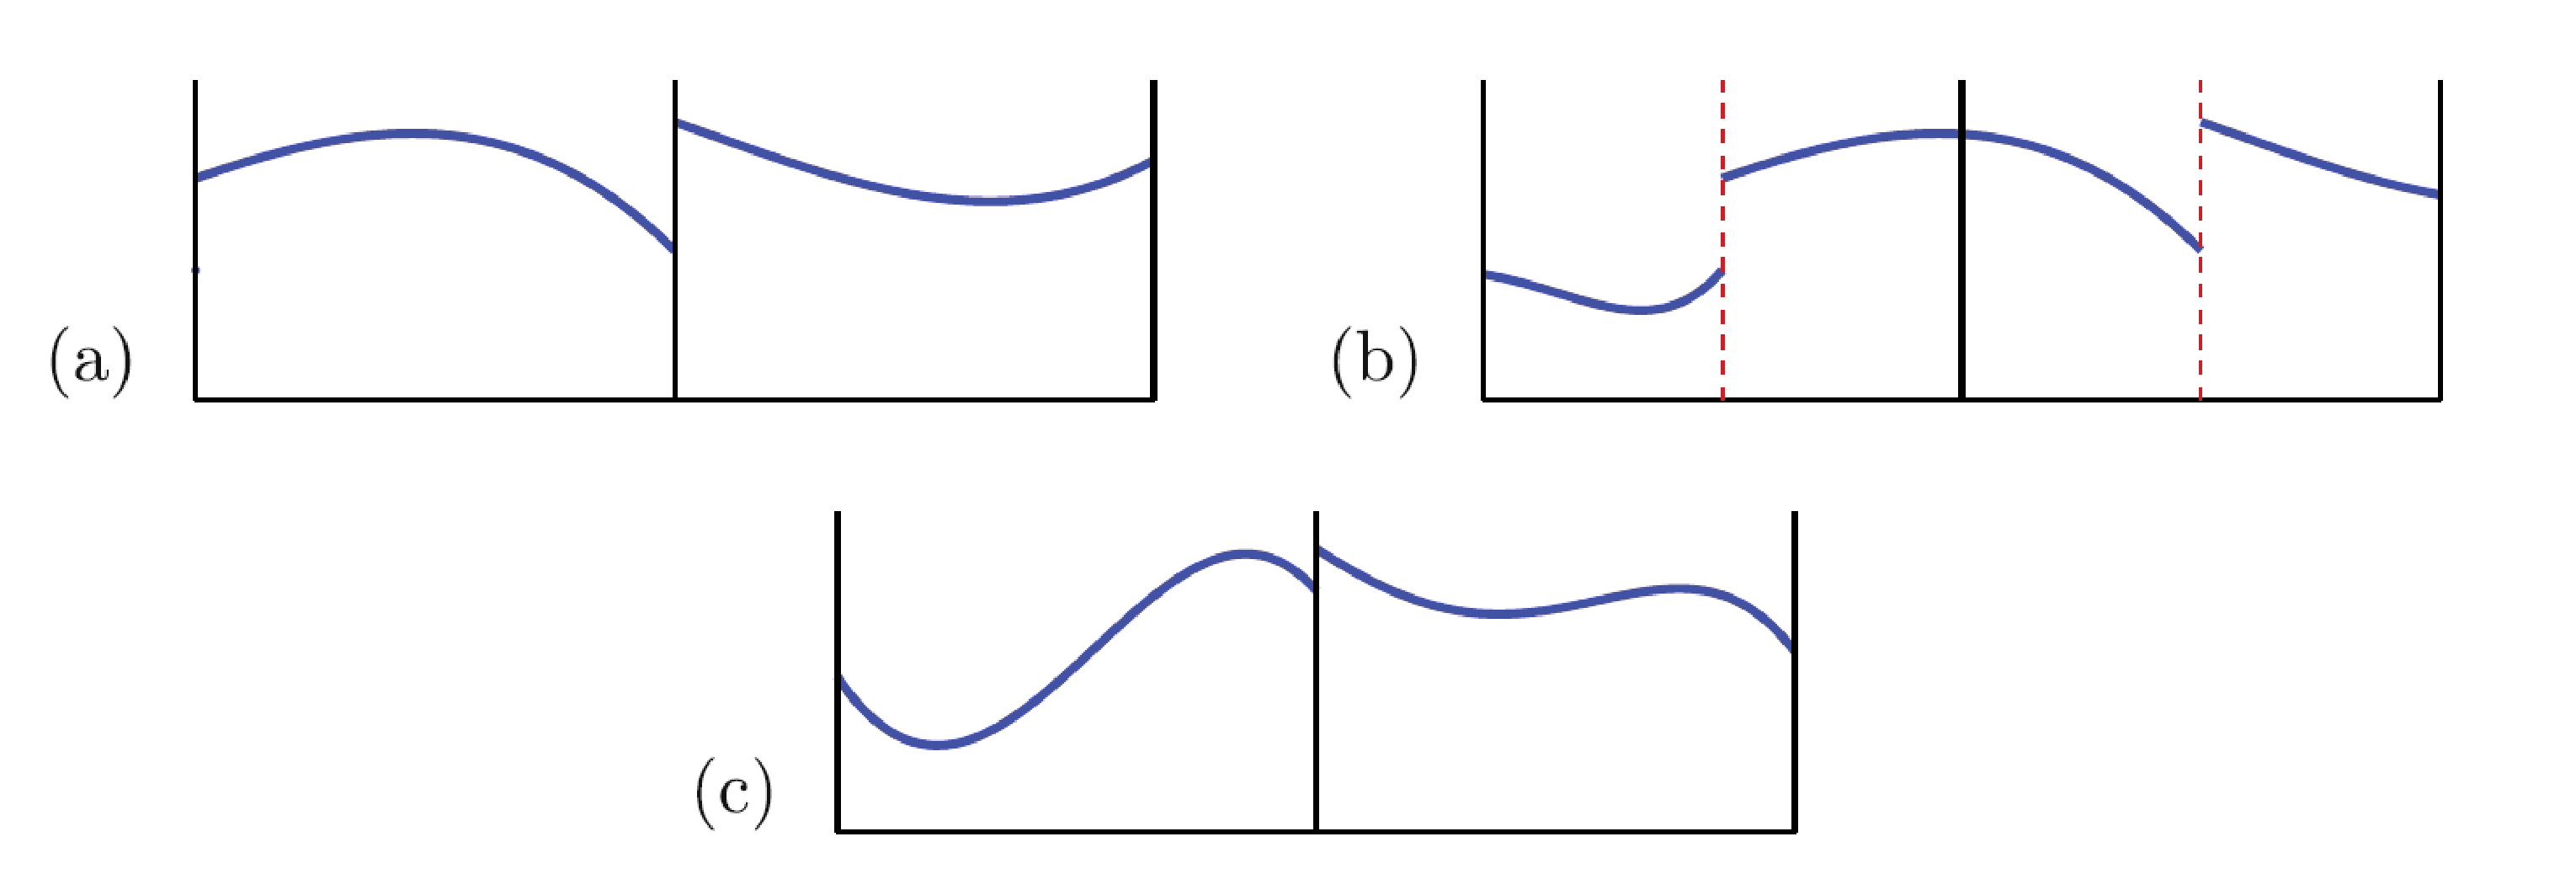
\includegraphics[width=0.9\textwidth]{graphics/DG.eps}
  \caption{In a discontinuous-Galerking (DG) method, cells (finite elements) are ascribed a functional form by chosen basis functions which are weighted by a set of coefficients that describe the density $f$; there is no enforcement of continuity from one cell to the next. In panel (a), initial data is shown for two cells. Panel (b) illustrates the exact advection of the solution, and panel (c) is the final processed result after a time step where the exact evolution in panel (b) is re-projected back onto the basis in for each cell \cite{Rossmanith11}.}
  \label{fig:Rossmanith_fig1}
\end{figure}

\noindent After the advection phase, the cells are smoothly remapped through an integral operation over the basis functions.

On the lower order extreme, the simplest parametrization of the profile is an $n$-dimensional Dirac delta function representation for each of the $n$ dimensions of the considered phase space (zero size particle, ZSP), where the appropriate remapping rule of an MC at its postpoint to the Eulerian grid is the \emph{nearest grid point} (NGP) assignment (the ZSP-NGP scheme). Such a trivialization of the distribution function of each MC leads to significant numerical error and unphysical artifacts such as amplified staircasing (as compared to higher order modeling) in the approximation of smooth curves (e.g. consider a Coulomb potential of a single charged particle) \cite{Birdsall69}.

Here, we take the density of any MC to be uniform in configurational space, which is convected according to a cell-centered velocity assignment so that we can regard the velocity space profile to be made up of a collection of Dirac delta functions.\label{page:density_is_constant} As for the shape of the moving cell itself, it is natural to take the Cartesian product of the sets of values that correspond to those subdomains in both configuration and velocity spaces that span the volume of each cell. That is, we have the direct product of two convex polyhedra \cite{Guclu12}, which more specifically produces a set of moving cells (Lagrangian mesh) represented as a collection of $n$-dimensional hypercubes ($n$-cube, or ``measure polytope''), whose union is equal to the problem domain $\mathbb{R}_x^{d_x} \times \mathbb{R}_v^{d_v}$. In graph theory, an $n$-cube skeleton is denoted by $Q_n$, where $n$ denotes both the number of vertices in the object and the corresponding dimension. In geometry, we refer to the solid $n$-cube by a label $\gamma_n$.  For the constant velocity, one-dimensional case (advection equation), the MC is a line segment (1-cube, $\gamma_1$). For the 1D-1V case, a 2-cube ($\gamma_2$, rectangle) describes the MC. In $n$-dimensions, the MC is an $n$-cube ($\gamma_n$).

The remapping rule to the Eulerian grid is executed at the end of a ballistic move (\ref{enum:Lgn_step}). To make the remap assignment specific, we take the problem domain in phase space ($\vec{x}, \vec{v}$) to be partitioned into cells $C_{ij}$ labelled by their centroids ($\vec{x}_i, \vec{v}_j$) such that $\cup C_{ij} = \Omega$ (the formal discrete problem in all detail is presented in section \ref{sec:The_discrete_problem}). The particle number $N_{MC}$ of the moving cells originating from a centroid ($\vec{x}_{0},\vec{v}_{0}$) are distributed among all such destination cells $\{C_{ij}\}$ in proportion to the phase space volume overlap of the fixed cells with that of the final (exact) location of the MC at the end of a time step, which is generally not an integral shift on the grid (figure \ref{fig:remap_rule}). If we consider the set all of all MCs $C_{i'j'}$ originating from centroids $(\vec{x}_{i'},\vec{v}_{j'})$, each with a particle number $N_{i'j'}$, we have the update in number $N_{ij}$ for every Eulerian cell $C_{ij}$:

\begin{equation}\label{eq:N_MC_update}N_{ij}\, +\hspace{-.3em}= \zeta_{i'j'\to ij}N_{i'j'} \quad \colon \quad \forall (i,j),(i',j')\in \boldsymbol{N}\oplus\boldsymbol{N}'\end{equation}

$$\textrm{where }\, 0 \leq\zeta_{i'j'\to ij}\leq 1 \, \textrm{and the grid index domain is given by } \boldsymbol{N} = \boldsymbol{N}' = \mathbb{N}_x \times \mathbb{N}_v$$

\begin{figure}[h!]
  \centering
    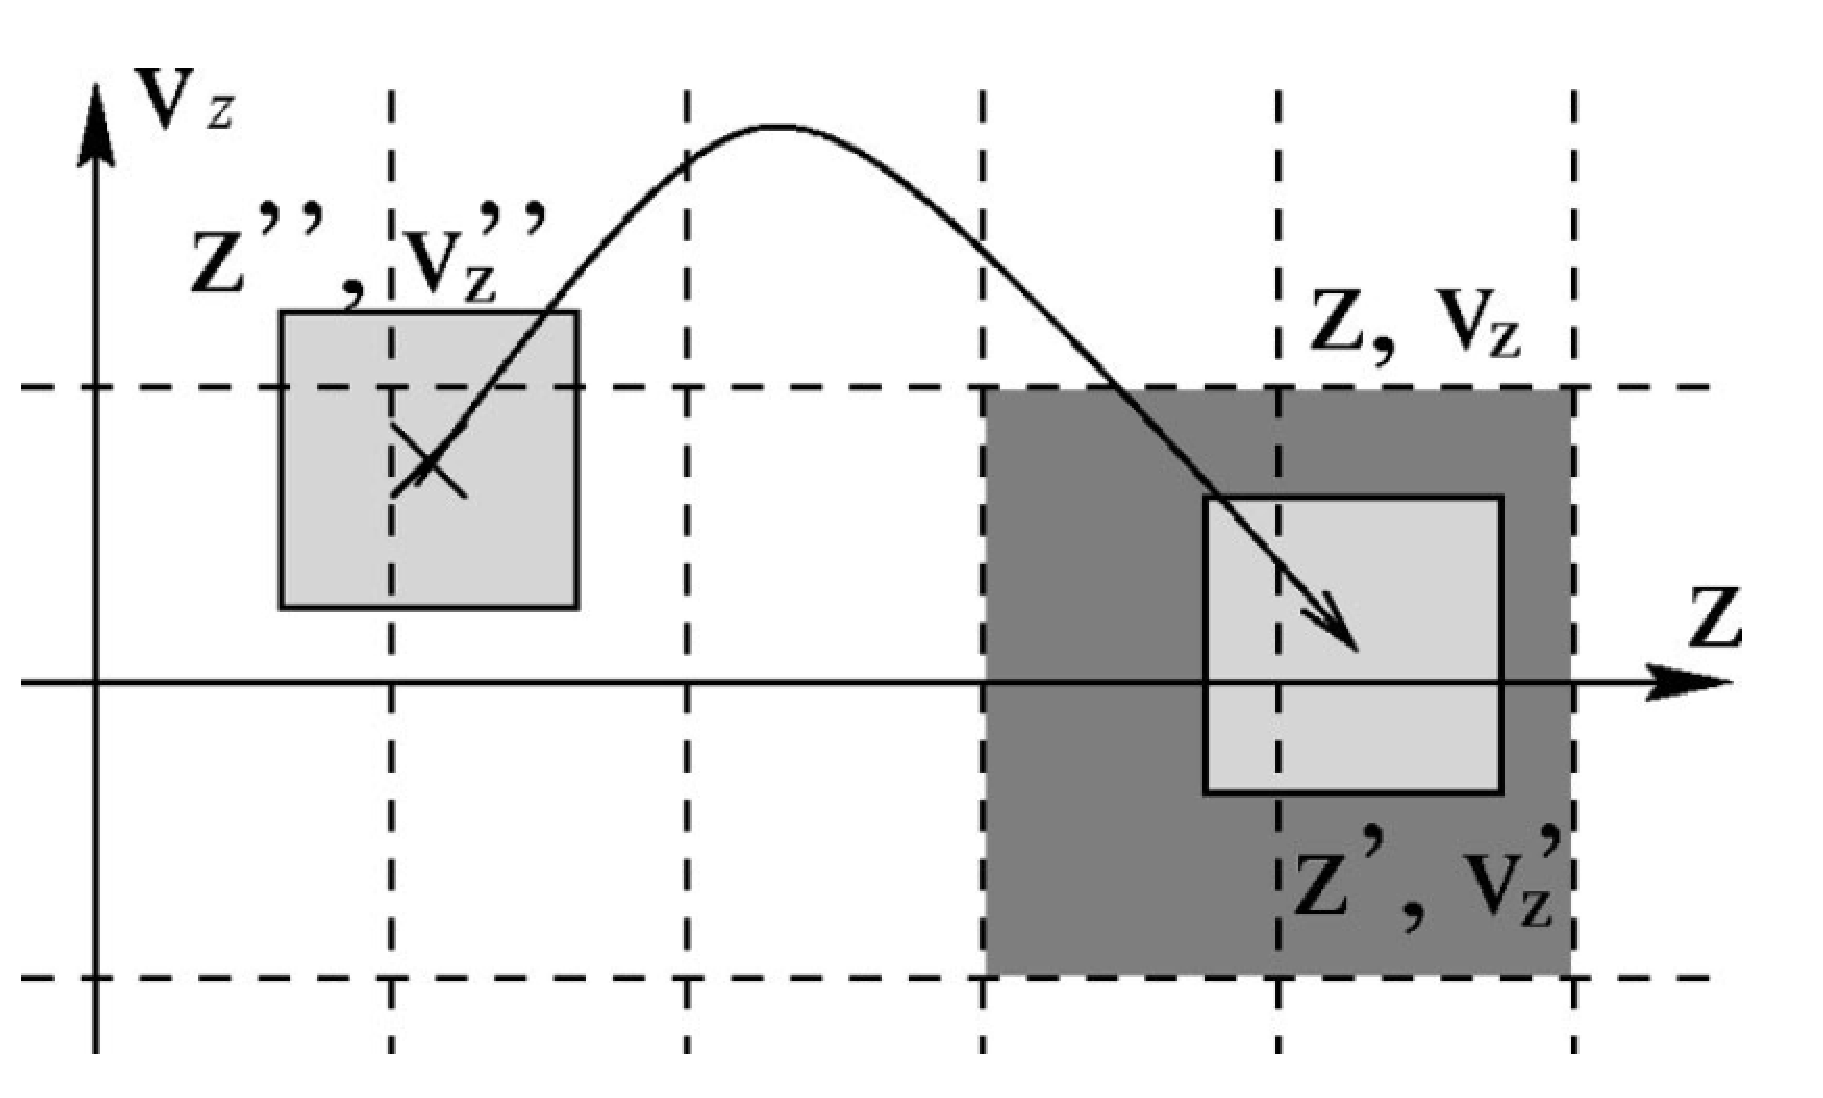
\includegraphics[width=0.45\textwidth]{graphics/remap_rule}
  \caption{A moving cell  with $(z'',v_z'')$ is propogated to a final location marked by $(z,v_z)$, which overlaps four cells (dotted outlines) in this 2D phase space. The CS remapping rule assigns the proportion of the MC to each overlapped cell according to its physical area overlap with the grid cells \cite[p.3162]{Feng00}.}
  \label{fig:remap_rule}
\end{figure}

\noindent The index sets $\mathbb{N}_x$ and $\mathbb{N}_v$ correspond to the indices enumerating cell-centers $(\vec{x}_i,\vec{v}_j)$ in the phase space $\mathbb{R}_x\times\mathbb{R}_v$ (e.g. $\mathbb{N}_x = \{i \colon \vec{x}_i\in\mathbb{R}_x \,\text{for all } i\in\mathbb{N}_0)\}$. The object $+\hspace{-.3em}=$ is the increment operator, defined such that $a\, +\hspace{-.3em}= b$ is interpreted as $a = a + b$. The quantity $\zeta_{i'j'\to ij}$ is the fraction of a moving cell $C_{i'j'}$ appropriated to a fixed cell $C_{ij}$. In general, this fraction changes from one time step to the next. This fraction $\zeta_{i'j'\to ij}$ is shown just below to correspond to the overlap fraction of each MC with phase space volume $\Gamma_{MC} \equiv \Gamma_{i'j'}$ relative to the fixed cells of volume $\Gamma_{ij}$. \cite{Birdsall69,Guclu12,Hitchon89}. This may be seen by writing the mapping statement from one MC, $C_{MC} \equiv C_{i'j'}$, to a single overlapped cell $C_{ij}$ on the Eulerian grid. This rule can then be looped over all MCs to remap the entire Lagrangian mesh to the Eulerian grid.

\begin{eqnarray*}
N_{ij} & +\hspace{-.3em}= & \int\limits_{C_{ij}} d^3\vec{x} d^3\vec{v}\, f_{MC}(t,\vec{x},\vec{v})\\
&&\\
& \phantom{+\hspace{-.3em}}= &  f_{MC}(t,\vec{x}_{i'},\vec{v}_{j'}) \int\limits_{C_{ij}\cap C_{MC}} d^3\vec{x} d^3\vec{v} \\
&&\\
& \phantom{+\hspace{-.3em}}= &  f_{MC}(t,\vec{x}_{i'},\vec{v}_{j'}) (\Gamma_{ij}\cap\Gamma_{MC}) \\
&&\\
N_{ij}& +\hspace{-.3em}= &  \underbrace{f_{MC}(t,\vec{x}_{i'},\vec{v}_{j'}) \Gamma_{MC}}_{N_{i'j'}} \underbrace{\frac{(\Gamma_{ij}\cap\Gamma_{MC})}{\Gamma_{MC}}}_{\zeta_{i'j'\to ij}} ,\qquad (i',j') \textrm{ denotes the MC}\\
&&\\
N_{ij} & +\hspace{-.3em}= & \zeta_{i'j'\to ij}N_{i'j'}
\end{eqnarray*}

\noindent Which is the same as equation \eqref{eq:N_MC_update}. The second equality follows from the choice that $f_{MC}$ is constant, and thus the integral results in only the total volume in phase space that overlaps. It is obvious from the definition of $\zeta_{i'j'\to ij}$

$$\zeta_{i'j'\to ij} = \frac{(\Gamma_{i'j'}\cap\Gamma_{ij})}{\Gamma_{i'j'}}$$

\noindent that each fraction $\zeta_{i'j'\to ij}$ for a given MC $C_{i'j'}$ sum to unity.

$$\sum_{i\in\mathbb{N}_x} \sum_{j\in\mathbb{N}_v} \zeta_{i'j'\to ij} = \sum_{i\in\mathbb{N}_x}\sum_{j\in\mathbb{N}_v} \frac{(\Gamma_{i'j'}\cap\Gamma_{ij})}{\Gamma_{i'j'}} = \frac{\Gamma_{i'j'}}{\Gamma_{i'j'}} = 1$$

Thus, the the mass is ensured to be conserved through the time stepping procedure. However, this remap assignment has the consequence of producing significant numerical diffusion as is now clear in view of the form the rule takes above (figure \ref{fig:ClassicCS_diffusion}).

\begin{figure}[h!]
  \centering
    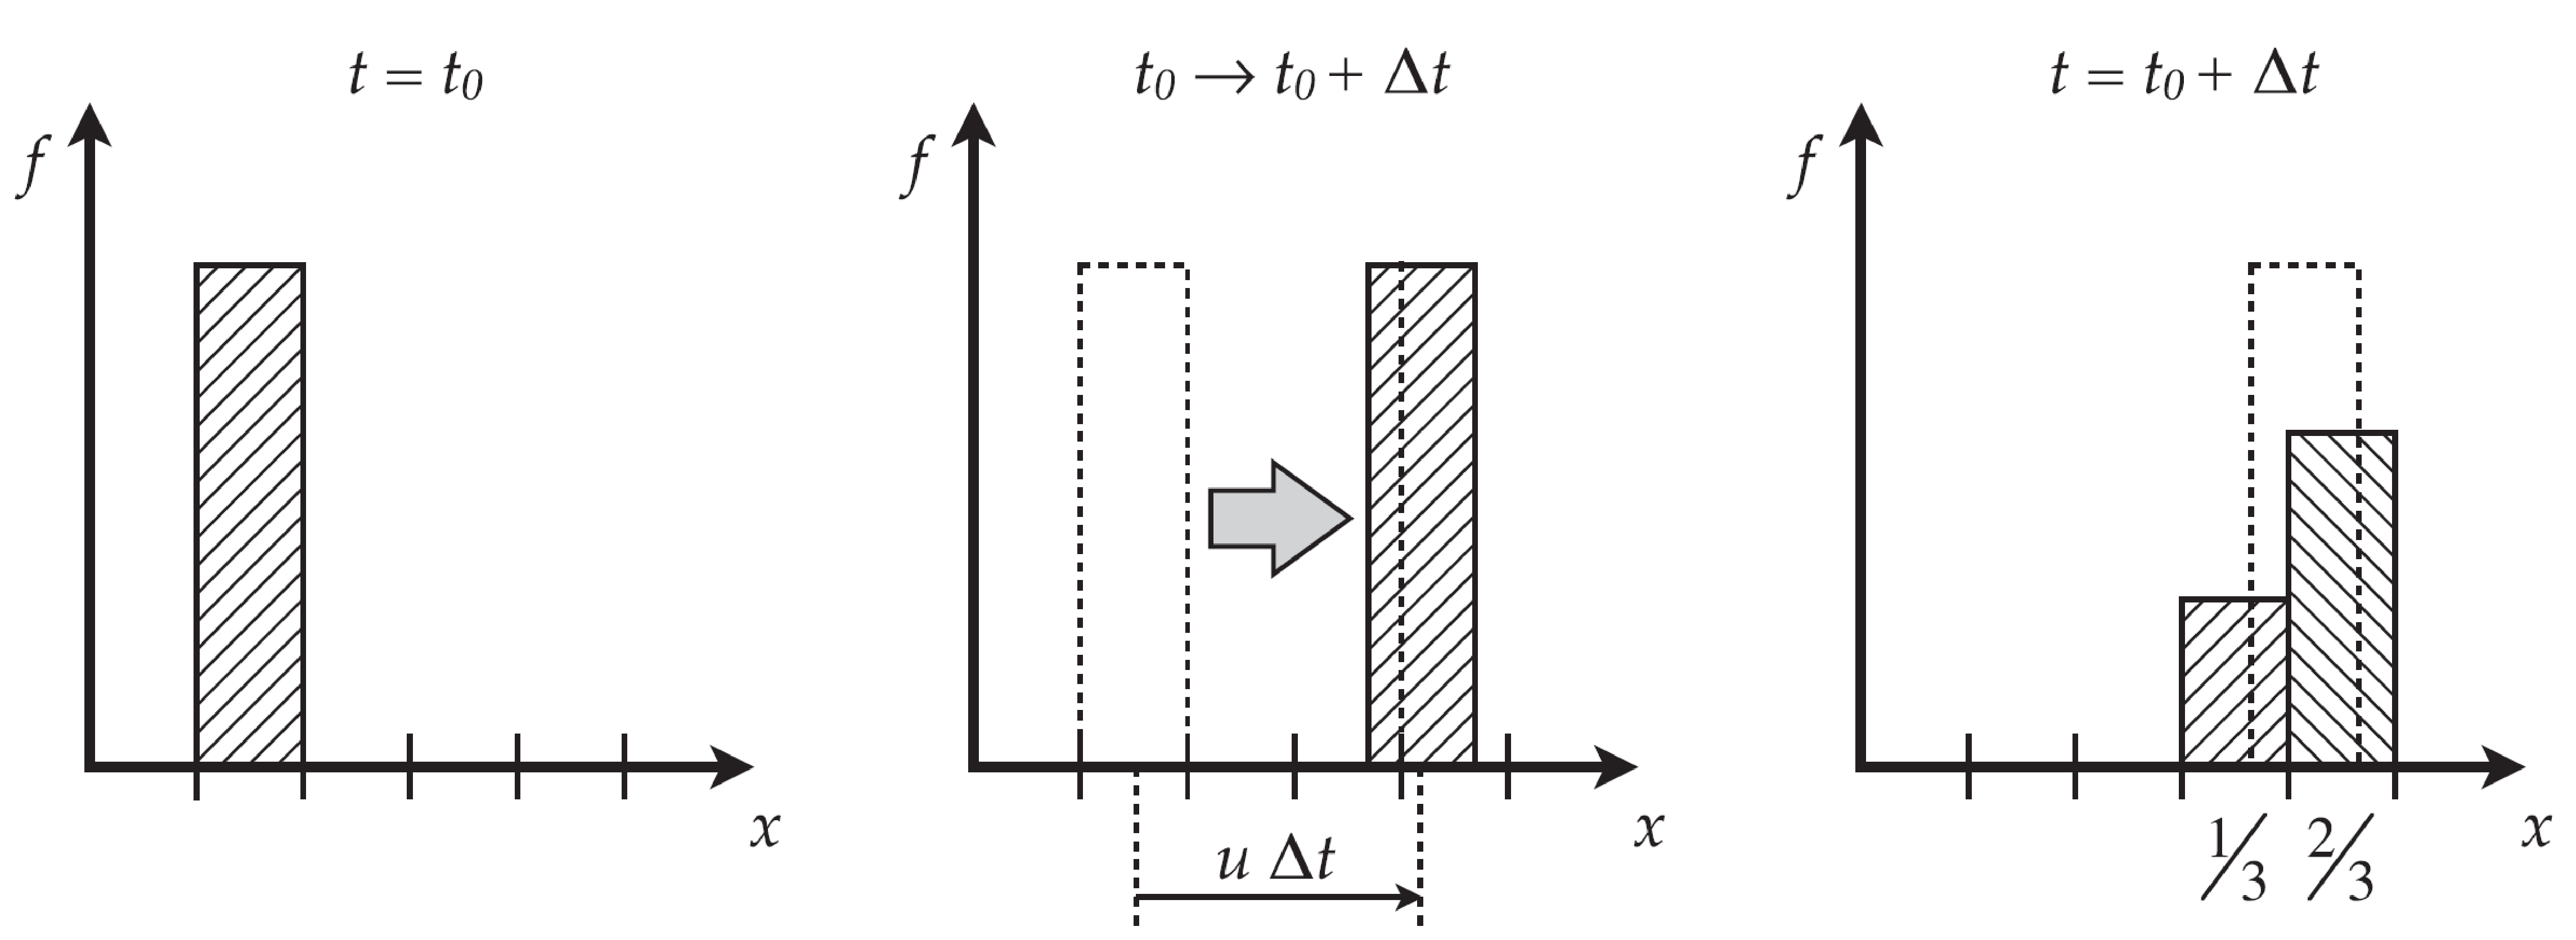
\includegraphics[width=0.75\textwidth]{graphics/ClassicCS_diffusion}
  \caption{A one-dimensional illustration is shown of the remap assignment where the MC starting at a cell center has been pushed with a speed $u$ towards the right that does not coincide exactly with only one cell, thus the remapping rule is employed as shown in frame 3. The result is an artificial spreading of the density across two continguous cells. The effect compounds as time marching continues for all points in space, so that the overall effect is diffusion \cite[p.3293]{Guclu12}.}
  \label{fig:ClassicCS_diffusion}
\end{figure}

This is a statement that every particle from the moving cell $C_{MC} \equiv C_{i'j'}$ is deposited to a cell $C_{ij}$ on the Eulerian grid, i.e. conservation of particle number. Note, that this rule introduces an allocation in phase space that is not automatically consistent with, for example, energy conservation. If desired, energy conservation can be implemented in the scheme above, e.g. Feng et. al \cite{Feng00}, by tying the velocity volume overlap fraction to an energy conservation statement. This is conveniently implemented by transforming to an energy mesh in favor of the velocity mesh for the remapping step so that factors pertaining to the kinetic energy $v^2$ replace the velocity factors $v$ in the fraction prescribed above. Notwithstanding, the approach in this research will be to reduce the remap error in velocity and configurational space so that the targeted consequence of this accuracy approximately conserves energy, or at least possess no secular increase in energy with respect to time stepping. An implementation of the Classic CS is given in algorithm \emph{\hyperlink{alg:1}{1}}, which is presented after the discrete problem is introduced (section \ref{sec:The_discrete_problem}).


\section{Higher order convected scheme}\label{sec:Higher_order_convected_scheme}

\indent\indent The classic convected scheme is first order accurate in space. We follow the workup presented by G\"{u}\c{c}lu \cite{Guclu14} to develop a higher order method of the convected scheme (CS) for a uniform velocity $v$ of the one-dimensional advection equation \eqref{eq:Advection_1D}:

$$\frac{\partial f}{\partial t} + v\frac{\partial f}{\partial x} = 0 \label{eq:Advection_1D} , \qquad x\in\mathcal{D}, \quad t \in (0,T]$$

\noindent And, subsequently inform how to use these high order solutions as building blocks to solve more complicated equations (e.g. with an acceleration term, and higher dimensions). Thus, the stepthrough is to advect density packets $f$ at each location $x$ along characteristics:

$$f(x,t + \Delta t) = f(x - v\Delta t, t)$$

\noindent which must then be remapped to the Eulerian grid according to the fractional overlap in cells. The displacement of each MC can equivalently be described by the number of grid points $\mathcal{C}$ the cell-center of an MC traverses in a time step. This normalized displacement is known as the Courant-Friedrichs-Lewy (CFL) parameter:

\begin{equation}\mathcal{C} \coloneqq \frac{v\Delta t}{\Delta x} =  S + \alpha , \qquad S\in\mathbb{Z}, \alpha\in(-1,1)\label{eq:CFL_first}\end{equation}

\noindent where $\Delta x$ is the spacing between grid points. Here, we make a point to emphasize the quantity $\alpha$ is a relative (fractional) distance between the MC postpoint and the nearest neighbor grid point. This fraction is related to the aforementioned area overlap fraction $\zeta$, but not the same. According to this decomposition, it is shown in section \ref{sec:The_discrete_problem} that after pushing a density packet by $S$ grid points, the CS remap update for the advection equation is given by:

 \begin{equation}
\label{eq:CS_update_FD_alpha}
 (f_{i+S}^{n+1})_{_{\mathrm{CS}}} =
  \begin{cases}
   \alpha_{i-1}^{n} f_{i-1}^n + (1 - \alpha_i^n)f_i^n & \text{if } v \geq 0 \\[0.75em]
   (1 + \alpha_i^n)f_i^n - \alpha_{i+1}^n f_{i+1}^n & \text{else }
  \end{cases}
\end{equation}

\noindent where we subscript the fractions $\alpha$ according to the cell they originated from. 

In the following, we provide the derivation of this prescription for the case of $v \geq 0$. At the conclusion, we discuss differences for the  $v < 0$ case and quote its corresponding result. The procedure amounts to matching Taylor series expansions of the exact solution with that of the CS update statement up to an order $\mathcal{O}(\Delta x^N)$, so that the local truncation error (LTE) is at most of order $\mathcal{O}(\Delta x^{N+1})$. Thus, we adopt the definition that an $N$th order method is accurate up to order $\mathcal{O}(\Delta x^N)$. After a proper ansatz is made, the problem reduces to seeking higher order corrections to only the fractional part $\alpha$ of the CFL number, as the integer shift $S$ presents no source of error for the remapping.

Thus, we analyze how to increase the accuracy of the remap assignment after shifting an MC by $S$ cells in general. Recall that $\alpha$ is the fractional distance measured between the cell-center of the MC with respect to the nearest Eulerian grid point such that $S$ and $\alpha$ are of the same sign. To clearly distinguish between corrected and uncorrected terms, we swap labels so that $\alpha$ indicates the uncorrected term and $U$ denotes the corresponding corrected version. The determination of the form of $U$ is the objective of this section. In this way, eq. \eqref{eq:CFL_first} becomes,

$$\mathcal{C} \coloneqq S + U, \qquad S\in\mathbb{Z},\, U\in (-1,1)$$

\noindent The Courant parameter $\mathcal{C}$ is a dimensionless displacement $\mathcal{C} \coloneqq v\Delta t / \Delta x$, and thus so are $S$ and $U$; however, we can equivalently view these terms as normalized velocities, e.g.

$$U \coloneqq \frac{v\Delta t}{\Delta x} - S = [v + \tilde{v} (t,x)]\frac{\Delta t}{\Delta x} - S = \alpha + \tilde{\alpha}(t,x)$$

\noindent where we assert an additional perturbation $\tilde{v}$ is present at higher orders to correct the velocity $v$ so that the final position of an MC is more optimal for the convected scheme. These velocities are nondimensionalized by the grid velocity $\Delta x / \Delta t$. Thus, it makes sense to speak of corrected normalized fluxes of the form $U(t,x)f(t,x)$. In the absence of higher order corrections, the  $U(t,x) = \alpha$ for all time. G\"{u}\c{c}lu refers to the term  $\tilde{\alpha}(t,x)$ above as an \emph{anti-diffusive correction} with the admission that strictly the term encompasses higher order effects should the method be extended to higher order $N$. No matter the form these correction terms take, they have no bearing on particle number conservation. From the update \eqref{eq:CS_update_FD_alpha}, we see that

$$\sum_i f_i^{n+1} = \sum_i f_{i+S}^{n+1} = \sum_i [U_{i-1}^n f_{i-1}^n + (1 - U_i^n) f_i^k] = \underbrace{\sum_i U_{i-1}^n f_{i-1}^n - \sum_i U_i^n f_i^n}_{=\,0} + \sum_i f_i^k = \sum_i f^n_i$$

The anti-diffusive correction adjusts the postpoint of the trajectory within its cell after a push along its characteristics so that a more \emph{optimal} fraction $U$ is used in the remapping step with respect to the convected scheme. That is, each MC is exactly convected by $\mathcal{C} = S + \alpha$, however the process of dispersing the density among neighboring grid points using the fraction $\alpha$ caps the accuracy at $\mathcal{O}(\Delta x^2)$ given the discreteness of the mesh \cite{Besse08}. Thus, the ``corrected'' value $U$ is not a correction to the position of the MC inasmuch as it is a modification to the fraction $\alpha$ to produce the optimal fraction $U$ so that the CS algorithm \emph{performs} at a higher level than its first order stencil permits. This notion is emphasized by recognizing the convected scheme update for a uniform velocity can be written as an upwind finite difference scheme (eq. \eqref{eq:CS_update_FD}).

For the case of a single uniform speed $v$, it is easily seen that only two loaded prepoints $i$ and $i\pm 1$ are mapped onto the grid point $i+S$, with the proportion $(1 \mp U_{i})$ and $(\pm U_{i\mp 1})$, respectively. Choosing the top sign corresponds to $v \geq 0$ whereas the bottom sign pertains to the case $v < 0$. Thus, \eqref{eq:CS_update_FD_alpha} amounts to:

\begin{equation}
\label{eq:CS_update_FD}
 (f_{i+S}^{n+1})_{_{\mathrm{CS}}} =
  \begin{cases}
   U_{i-1}^{n} f_{i-1}^n + (1 - U_i^n)f_i^n & \text{if } v \geq 0 \\[0.75em]
   (1 + U_i^n)f_i^n - U_{i+1}^n f_{i+1}^n & \text{else }
  \end{cases}
\end{equation}

\noindent Where, as noted, there is zero remapping error associated with translating an MC by an integer number of cells, thus the remapping assignment above is reported at a general shifted location $i + S$, which is subject to boundary conditions.

To find the form of the corrections $U_i$ above, we begin by expanding all terms in \eqref{eq:CS_update_FD} for $v \geq 0$ about the point $(t,x)$ up to order $\mathcal{O}(\Delta x^N)$. The left-hand term becomes:

$$U_{i-1}^n f_{i-1}^n  =  U(t,x - \Delta x) f(t,x - \Delta x) =  U(t,x)f(t,x) + \sum_{p = 1}^{N} \frac{(-\Delta x)^p}{p!}\frac{\partial^p(Uf)}{\partial x^p}\biggr|_{(t,x)} + \mathcal{O}(\Delta x^{N+1})$$

\noindent so that the CS update reads

\begin{eqnarray}
(f^{n+1}_{i+S})_{_{\mathrm{CS}}} & = & U_{i-1}^{n} f_{i-1}^n + (1 - U_i^n)f_i^n \nonumber \\[0.5em]
& = & \left(U(t,x)f(t,x) + \sum_{p = 1}^{N} \frac{(-\Delta x)^p}{p!}\frac{\partial^p(Uf)}{\partial x^p}\biggr|_{(t,x)
} + \mathcal{O}(\Delta x^{N+1})\right) + f(t,x) - U(t,x)f(t,x) \nonumber \\[0.5em]
(f^{n+1}_{i+S})_{_{\mathrm{CS}}} & = &  f(t,x) + \sum_{p = 1}^{N}\frac{(-\Delta x)^p}{p!}\frac{\partial^p(Uf)}{\partial x^p}\biggr|_{(t,x)} + \mathcal{O}(\Delta x^{N+1}) \label{eq:CS_update_expansion}
\end{eqnarray}

\noindent The exact solution is advected by $S + \alpha$ so that the following solution holds $f(t + \Delta t, x + S\Delta x) = f(t, x - \alpha \Delta x)$. Taylor expanding this solution, we see that

\begin{equation}
(f_{i+S}^{n+1})_{_{\mathrm{exact}}} = f(t + \Delta, x + S\Delta x)  =  f(t,x) + \sum_{p = 1}^{N}\alpha^p \frac{(-\Delta x)^p}{p!}\frac{\partial^p f}{\partial x^p}\biggr|_{(t,x)} + \mathcal{O}(\Delta x^{N+1}) \label{eq:f_exact_expansion}
\end{equation}

\noindent An $N$th order method ensures the local truncation error (LTE) is at greatest $\mathcal{O}(\Delta x^{N+1})$:

$$\mathrm{LTE}\,(t,x,\Delta x) \coloneqq f_{_{\mathrm{exact}}}(t + \Delta t,x + S\Delta x) - f_{_{\mathrm{CS}}}(t + \Delta t,x + S\Delta x) = \mathcal{O}(\Delta x^{N+1})$$

\noindent comparing eqs. \eqref{eq:CS_update_expansion} and \eqref{eq:f_exact_expansion}, we see the above equality implies

\begin{eqnarray*}
\mathrm{LTE}\,(t,x,\Delta x) & = &  \left(f(t,x) + \sum_{p = 1}^{N} \alpha^p \frac{(-\Delta x)^p}{p!}\frac{\partial^p f}{\partial x^p}\biggr|_{(t,x)}\right) - \left(f(t,x) + \sum_{p = 1}^{N} \frac{(-\Delta x)^p}{p!}\frac{\partial^p(Uf)}{\partial x^p}\biggr|_{(t,x)}\right) + \mathcal{O}(\Delta x^{N+1})\\[0.5em]
& = & \sum_{p = 1}^{N} \frac{(-\Delta x)^p}{p!}\alpha^p \frac{\partial^p f}{\partial x^p}\biggr|_{(t,x)} -\sum_{p = 1}^{N} \frac{(-\Delta x)^p}{p!} \frac{\partial^p(Uf)}{\partial x^p}\biggr|_{(t,x)} + \mathcal{O}(\Delta x^{N+1})\\[0.7em]
\mathrm{LTE}\,(t,x,\Delta x) & = &  \mathcal{O}(\Delta x^{N+1})
\end{eqnarray*}\\

\noindent provided that the following condition is met,

\begin{equation} \sum_{p = 1}^{N} \frac{(-\Delta x)^p}{p!}\alpha^p \frac{\partial^p f}{\partial x^p}\biggr|_{(t,x)} - \sum_{p = 1}^{N} \frac{(-\Delta x)^p}{p!}\frac{\partial^p(Uf)}{\partial x^p}\biggr|_{(t,x)} = 0\label{eq:CS_correction_order_conditions}
\end{equation}\\[0.1em]

To make further progress, \cite{Guclu14} proposes the following power series ansatz for the product $U(t,x)f(t,x)$, which we introduce as correct to order $\mathcal{O}(\Delta x^N)$ to ensure $N$th order accuracy is maintained:

\begin{equation}
U(t,x)f(t,x) \coloneqq \sum_{q = 0}^{N-1} \beta_q(\alpha )(-\Delta x)^q\frac{\partial^q f}{\partial x^q}\biggr|_{(t,x)} + \mathcal{O}(\Delta x^{N+1}) \label{eq:Uf_ansatz}
\end{equation}

\noindent Inserting this series into \eqref{eq:CS_correction_order_conditions}, the problem reduces to seeking coefficients $\beta_q(\alpha )$ that define the correction $U$. The right-hand term becomes:

\begin{eqnarray}
\sum_{p = 1}^{N} \frac{(-\Delta x)^p}{p!}\frac{\partial^p(Uf)}{\partial x^p}\biggr|_{(t,x)}  & = & \sum_{p = 1}^{N} \frac{(-\Delta x)^p}{p!}\left(\sum_{q = 0}^{N-1}  \beta_q(\alpha )(-\Delta x)^q\frac{\partial^q f}{\partial x^q}\biggr|_{(t,x)}\right) + \mathcal{O}(\Delta x^{N+1})\nonumber \\[0.3em]
& = & \sum_{p = 1}^{N}\sum_{q = 0}^{N-1}(-\Delta x)^{p+q}\frac{\beta_q(\alpha )}{p!} \frac{\partial^{p+q} f}{\partial x^{p+q}}\biggr|_{(t,x)} + \mathcal{O}(\Delta x^{N+1}) \label{eq:Double_summation_1}\\[0.3em]
\sum_{p = 1}^{N} \frac{(-\Delta x)^p}{p!}\frac{\partial^p(Uf)}{\partial x^p}\biggr|_{(t,x)} & = & \sum_{r = 1}^{N}\sum_{q = 0}^{r-1}(-\Delta x)^r\frac{\beta_q(\alpha )}{(r - q)!} \frac{\partial^r f}{\partial x^r}\biggr|_{(t,x)} + \mathcal{O}(\Delta x^{N+1}), \qquad r = p + q \label{eq:Double_summation_2}
\end{eqnarray}

\noindent The $\mathcal{O}(\Delta x^{N+1})$ term collects higher order terms that result from the combined terms of both sums. To prove the index change in the final equality, note for $p = 1, 2, \ldots, N$, $q = 0, 1, \ldots , N-1$, we have $r = p + q \Rightarrow p = r - q$, such that

$$\sum_{p = 1}^N\sum_{q = 0}^{N-1} \rightarrow \sum_{r - q = 1}^N\sum_{q = 0}^{N-1} = \sum_{r = q + 1}^N\sum_{q = 0}^{N-1}$$

\noindent The sum interchange is easily visualized in tabular form, where the elements are represented as entries and the double summation amounts to adding all elements together. \\[0.3em]

%this is a really terrible way to set up the table, I know. I was just working for spacing and I did not read any documentation on this package \makecell so was just guessing

\begin{landscape}
\begin{table}[h!]
\begin{tabular}{|M{4cm}|M{4cm}|M{4cm}|M{4cm}|M{0.4cm}|M{5cm}|N}\hline
\diaghead{\theadfont fdsjafidsjfidsjfodfsafasdfdsad}%
  {$\phantom{r =}\mathlarger{\mathlarger{\mathlarger{\mathlarger{r = q + 1}}}}$}{\\$\mathlarger{\mathlarger{\mathlarger{\mathlarger{q}}}}\phantom{edfsa}$}&
$\mathlarger{\mathlarger{\mathlarger{0}}}$ & $\mathlarger{\mathlarger{\mathlarger{1}}}$ & $\mathlarger{\mathlarger{\mathlarger{2}}}$ & \ldots & $\mathlarger{\mathlarger{\mathlarger{N-1}}}$ \\ \hline

$\mathlarger{\mathlarger{\mathlarger{1}}}$ & $$(-\Delta x)^1\frac{\beta_0(\alpha )}{(1 - 0)!}\frac{\partial^1 f}{\partial x^1}$$ & \cellcolor{blue!20}\ldots & \cellcolor{blue!20}\ldots &  \cellcolor{blue!20}\ldots& \cellcolor{blue!20}\ldots &\\[25pt] \hline

$\mathlarger{\mathlarger{\mathlarger{2}}}$ & $$(-\Delta x)^2\frac{\beta_0(\alpha )}{(2 - 0)!}\frac{\partial^2 f}{\partial x^2}$$ & $$(-\Delta x)^2\frac{\beta_1(\alpha )}{(2 - 1)!}\frac{\partial^2 f}{\partial x^2}$$ & \cellcolor{blue!20}\ldots  &\cellcolor{blue!20} \ldots & \cellcolor{blue!20}\ldots  &\\[25pt] \hline

 $\mathlarger{\mathlarger{\mathlarger{3}}}$& $$(-\Delta x)^3\frac{\beta_0(\alpha )}{(3 - 0)!}\frac{\partial^3 f}{\partial x^3}$$ & $$(-\Delta x)^3\frac{\beta_1(\alpha )}{(3 - 1)!}\frac{\partial^3 f}{\partial x^3}$$ & $$(-\Delta x)^3\frac{\beta_2(\alpha )}{(3 - 2)!}\frac{\partial^3 f}{\partial x^3}$$ &\cellcolor{blue!20}\ldots & \cellcolor{blue!20}\ldots & \\[25pt] \hline

 \ldots & \ldots & \ldots & \ldots & \ldots  & \cellcolor{blue!20}\ldots &\\[25pt] \hline

$\mathlarger{\mathlarger{\mathlarger{N}}}$ & $$(-\Delta x)^N\frac{\beta_0(\alpha )}{(N - 0)!}\frac{\partial^N f}{\partial x^N}$$ &  $$(-\Delta x)^N\frac{\beta_1(\alpha )}{(N - 1)!}\frac{\partial^N f}{\partial x^N}$$ &  $$(-\Delta x)^N\frac{\beta_2(\alpha )}{(N - 2)!}\frac{\partial^N f}{\partial x^N}$$ & \ldots &$$(-\Delta x)^N\frac{\beta_{N-1}(\alpha )}{[N - (N - 1)]!}\frac{\partial^N f}{\partial x^N}$$ &\\[25pt] \hline

\end{tabular}
  \caption{Visualizing the double sum of eq. \eqref{eq:Double_summation_1} as entries in a table. The top row is over the $q = 0, 1, \ldots , N-1$, whereas the left-most column enumerates $p = 1, 2, \ldots, N$, which has been put in terms of $r = p + q$ in order to discern the limits of a double sum in terms of $q$ and $r$ alone. The colored cells indicate entries where $r < q + 1$, which are not terms that appear in the summation. Derivatives are evaluated at the point $(t,x)$.}
\end{table}
\end{landscape}

Thus, we can see by adding up all entries in the table, the following set of limits are equivalent:

$$\sum_{p = 1}^N\sum_{q = 0}^{N-1} = \sum_{r = 1}^N\sum_{q = 0}^{r-1} $$

\noindent which is the sum we have written in eq. \eqref{eq:Double_summation_2}. For transparency, relabel the dummy index $r$ as $p$, so that the same equation can be written as:

$$\sum_{p = 1}^{N} \frac{(-\Delta x)^p}{p!}\frac{\partial^p(Uf)}{\partial x^p}\biggr|_{(t,x)}  =  \sum_{p = 1}^{N}\sum_{q = 0}^{p-1}(-\Delta x)^p\frac{\beta_q(\alpha )}{(p - q)!} \frac{\partial^p f}{\partial x^p}\biggr|_{(t,x)} + \mathcal{O}(\Delta x^{N+1})$$.

\noindent Thus, the order condition \eqref{eq:CS_correction_order_conditions}

\begin{eqnarray*} \sum_{p = 1}^{N} \frac{(-\Delta x)^p}{p!} \alpha^p \frac{\partial^p f}{\partial x^p}\biggr|_{(t,x)} - \sum_{p = 1}^{N} \frac{(-\Delta x)^p}{p!}\frac{\partial^p(Uf)}{\partial x^p}\biggr|_{(t,x)} & = &  0\\[0.3em]
 \sum_{p = 1}^{N} \frac{(-\Delta x)^p}{p!}\alpha^p \frac{\partial^p f}{\partial x^p}\biggr|_{(t,x)} - \sum_{p = 1}^{N}\sum_{q = 0}^{p-1}(-\Delta x)^p\frac{\beta_q(\alpha )}{(p - q)!} \frac{\partial^p f}{\partial x^p}\biggr|_{(t,x)}   & = & 0\\[0.3em]
  \sum_{p = 1}^{N} (-\Delta x)^p\left(\frac{\alpha^p}{p!}  - \sum_{q = 0}^{p-1}\frac{\beta_q(\alpha )}{(p - q)!}\right)\frac{\partial^p f}{\partial x^p}\biggr|_{(t,x)}  & = & 0
\end{eqnarray*}\\[0.1em]

\noindent So, that the coefficient functions $\beta_q(\alpha )$ are defined by the relationship

\begin{equation}
\sum_{q = 0}^{p-1}\frac{\beta_q(\alpha )}{(p - q)!} = \frac{\alpha^p}{p!} \label{eq:beta_definition}
\end{equation}

\noindent The set of equations produced from \eqref{eq:beta_definition} constitute a matrix system with a lower triangular coefficient matrix, thus it is easy to verify through forward substitution that the following recursive definitions hold \cite{Guclu14}, where we also show the result for $v < 0$ for completeness:\\[0.5em]

\begin{equation}\beta_0(\alpha )  =  \alpha ,\qquad \qquad \qquad \,\,\,\qquad \forall\, v\in\mathbb{R}\end{equation}

\begin{equation}
\label{eq:beta_q}
\beta_p(\alpha ) =
\begin{dcases*}
\frac{\alpha^{p+1}}{(p+1)!} - \sum_{q = 0}^{p - 1}\frac{\beta_q(\alpha )}{(p + 1 - q)!} &
for $v \geq 0, \, p = 1, 2, \ldots, $\\
\frac{\alpha^{p+1}}{(p+1)!} - \sum_{q = 0}^{p - 1}(-1)^{p+q}\frac{\beta_q(\alpha )}{(p + 1 - q)!} &
for $v < 0, \, p = 1, 2, \ldots, $
\end{dcases*}
\end{equation}

\noindent The result for $v < 0$ follows similarly, where we begin from the latter form of the CS update \eqref{eq:CS_update_FD}, and assert an identical power series \eqref{eq:Uf_ansatz} for the product $U(t,x)f(t,x)$. G\"{u}\c{c}lu presents a series of equivalent formulations for these coefficients. Namely, it is shown that these coefficient functions $\beta_p(\alpha )$ are scaled combinations of Bernoulli numbers, and may be computed either by consult of a table of Bernoulli numbers, or extracted from specific values of the Bernoulli polynomials \cite{Guclu14}.

The optimized fractional displacement $U_N$ is most gently introduced by computing its $N$th order accurate flux $[U_N(t,x)f(t,x)] \equiv [Uf]_i^n$ from the ansatz \eqref{eq:Uf_ansatz}

\begin{equation}\boxed{U_N(t,x)f(t,x) \coloneqq \sum_{q = 0}^{N-1} \beta_q(\alpha )(-\Delta x)^q\frac{\partial^q f}{\partial x^q}\biggr|_{(t,x)} = \alpha f(t,x) + \sum_{q = 1}^{N-1} \beta_q(\alpha )(-\Delta x)^q\frac{\partial^q f}{\partial x^q}\biggr|_{(t,x)}}\label{eq:Uf}\end{equation}

\noindent defined such that $U(t,x)f(t,x) = U_N(t,x)f(t,x) + \mathcal{O}(\Delta x^{N+1})$. Thus, the above equation provides the form of the corrected terms that appear in \eqref{eq:CS_update_FD}. For brevity, the subscript $N$ will be suppressed given it is understood an exact value is beyond the means of a numerical calculation. By working with the normalized flux, we evade a direct source for numerical overflow. \emph{The implementation then requires $N-1$ derivatives of the distribution function $f(t,x)$ to create an $N$th order method} \label{pg:deriv_reqs}. In order to maintain the accuracy, the means of obtaining these derivatives must be at least of order $N$. For example, these derivatives can be estimated through finite differences with sufficient sized stencils relative to scheme (see the \emph{FD5} scheme in section \ref{subsec:FD_implementation}). Alternatively, a direct method applicable to periodic domains (as is the case considered) is to compute the derivatives in the Fourier domain (section \ref{subsubsec:Spectral_derivatives}) which are equivalent to $\mathcal{O}(N^2)$ algebraic operations on the distribution function whereafter an inverse can be taken to record the value of the derivative. The use of a discrete fast Fourier transforms (FFT) and its corresponding inverse operation (IFFT) reduces the computational cost to $\mathcal{O}(N\log_2N)$. In this way, the CS achieves spectral convergence as the truncation error rapidly approaches machine precision for orders of $N \gtrsim 20$ in double precision \cite{Guclu14}, hence this scheme is sometimes referred to as \emph{spectral CS} ($FN$ methods). However, for orders larger than approximately $N \approx 25$, high frequency white noise from the discrete transform process shows significant effect. Since the artificial noise is especially significant for low-level amplitudes, a low-pass filter can be incorporated in the implementation to reduce the pronounced numerical error for low amplitude densities. Using such a filter provides optimal orders between $20 \lesssim N \lesssim 25$ \cite{Guclu14}. We delay the detailed description of this implementation for a moment to discuss issues associated with applying the correction $U_N$ as a direct calculation of \eqref{eq:Uf}. 


\subsubsection{Design of a positivity and mass preserving limiter for the correction terms}

\indent \indent Applying the correction term \eqref{eq:Uf} requires a careful approach. As motivated above, one safeguard that can be taken is to forego the explicit calculation of $U_i^n$ in favor of keeping the product $[Uf]_i^n$ intact. This measure evades one means of numerical overflow given that the computation of $U_i^n$ according to eq. \eqref{eq:Uf} invariably involves division by small values of the density $f_i^n$ in sparse regions of phase space. However, there are still means by which the normalized flux $[Uf]_i^n$ can become either too large or otherwise erroneous. Notwithstanding, it is more direct to describe these remaining sources of error in terms of the problems they cause with the correction $U_i^n$ rather than the upwind flux $[Uf]_i^n$. Thus, we choose to introduce the issues in terms of their effect on $U_i^n$ below, and thereafter carryover their consequences to the flux in order to design a filter (or limiter) for the flux that ameliorates these problems \cite{Guclu14}.

The remaining sources of error pertain to $(1)$ the actual values of the $N-1$ derivatives themselves, and/or $(2)$ the accuracy of their numerical estimation. As concerns $(1)$, should the actual values of the derivatives be large relative to $f_i^n$, it can be the case that the computed correction $|U_i^n| > 1$ (cf. \eqref{eq:Uf}) so that it no longer presents a correction to the final position of an MC within the cell, but pushes it past the nearest cell-center. This violates the definition of the corrective term given that $U_i^n$ is a correction to a fraction $|\alpha_{i'\to i}^n| < 1$ which must demand that $|U_i^n| < 1$. The second point $(2)$ regards the fidelity of the derivative calculations. The numerical estimation of the derivatives will contain errors from undersampling if the mesh is not sufficiently resolved in the vicinity of regions of sharp changes due to not satisfying the Nyquist criterion. In this way, an overall erroneous $U_i^n$ value can result due to compounded error from unreliable derivative calculations from aliasing.

Finally, we mention that the sign is also not restricted in \eqref{eq:Uf}, so that given the previous discussion it is possible to create largely negative corrections $U_i^n$. Thus, an unrestrained application of the correction $U_i^n$ can conspire with the CS update \eqref{eq:CS_update_FD} to cause negative densities to evolve in time from an initially nonnegative distribution. Thus, a limiter needs to be designed to preserve two properties: $(1)$ The distribution function must maintain its positivity, and $(2)$ the term $U_i^n$ must not be so large that it pushes the MC past its nearest grid point. To motivate the stepthrough of the selection of an appropriate correction, we refer to the calculation of eq. \eqref{eq:Uf} as the \emph{nominal} correction $\tilde{U}_i^n$. Further, we choose to label the corresponding nominal normalized flux as $\Gamma_i^n = \tilde{U}_i^nf_{i'}^n$, as opposed to $[\tilde{U}f]_i^n$ to keep consistent track of the the density parcel $f_i^n$ that is first convected by the integer part of the Courant parameter to a location marked by $i'$ before it is allocated to cell centers according to the correction $\tilde{U}_i^n$. Tagging the density parcel in this way proves most direct with respect to implementing the algorithm.

According to the above two concerns, for $v \geq 0$ we must have:


\begin{enumerate}
\item \emph{Sign preservation}: $U_i^{n} \geq 0$ implies need to select a correction $U_i^{'n} = \max (0,\tilde{U}_i^n)$
\item \emph{Numerical limiting}: The correction $U_i^n \leq 1$ implies $U_i^n = \min (U_i^{'n},1)$
\end{enumerate}

\noindent Thus, the above two considerations design the following simple limiter, which are given in terms of both $U_i^n$ and the normalized flux $U_i^nf_{i'}^n$: \\[0.5em]

\noindent\noindent\begin{minipage}{0.45\textwidth}
\vspace{1em}$$U_i^n =
  \begin{cases}
    \min\, [ \max \,(0,\tilde{U}_i^n), 1]  & \text{if } v \geq 0 \\[1em]
    \max\, [ \min (-1,\tilde{U}_i^n), 0]       & \text{else}
  \end{cases}$$
\end{minipage}
\begin{minipage}{0.55\textwidth}
\begin{equation}\text{or }\,\,\,\,U_i^nf_{i'}^n =
  \begin{cases}
    \min \,[\max \,(0,\tilde{U}_i^nf_{i'}^n), f_i^n]  & \text{if } v \geq 0 \\[1em]
    \max \,[\min \,(-f_i^n, \tilde{U}_i^nf_{i'}^n), 0]    & \text{else}
  \end{cases}\label{eq:Uf_limiter}\end{equation}
\end{minipage}\\[1em]

\noindent The result for negative velocities ($v < 0$) has also been provided, which is arrived at through analogous considerations. Thus, an algorithm employing the above limiter ensures positivity preservation of the distribution function, as well as unphysical overcorrections. The general implementation for the higher order CS is provided in algorithm \emph{\hyperlink{alg:2}{2}}. These algorithms are given after the discrete problem is introduced in full (section \ref{sec:The_discrete_problem}).


\subsubsection{Windowed Fourier methods}\label{subsubsec:Windowed_Fourier_methods}

\indent\indent If the derivatives required for the correction \eqref{eq:Uf} are computed in the Fourier domain ($FN$ methods, section \ref{subsubsec:Spectral_derivatives}, \hyperlink{alg:3}{algorithm 3}), we note a clear concern for any Fourier-based method is the appearance of unphysical oscillations. Hence, the Fourier-based convected scheme methods are challenged in the presence of sharp boundaries given artifacts introduced by the Gibbs phenomenon. If the unphysical oscillations are left unchecked, they introduce additional error nonlocally and contaminate the global solution. A straightforward means to limit their extent in pervading the solution is to window the Fourier transform by use of an adequately designed low-pass filter \cite{Wei99, Sun05, Guclu14}. Following the motivation used by G.W. Wei and Sun et. al, a simple filter can be arrived at by considering the transform of the same function written in an equivalent manner. That is, realizing the Dirac delta function is the identity element for the convolution operation permits the following to be written:

\begin{equation}f(x) = (\delta * f)(x) = \int_{-\infty}^{\infty} \delta(x - X)f(X) dX\label{eq:delta_identity_convolution}\end{equation}

\noindent where the Dirac delta function is the kernel in this convolution statement. To realize the Dirac delta function on a computer, the class of wave packets $\delta_{\sigma,\Delta x}$ is chosen as an approximation, which analytically approaches the delta function in the limit,

\begin{equation}\lim_{\Delta x \rightarrow 0}\delta_{\sigma,\Delta x}(x) = \delta(x), \qquad \delta_{\sigma,\Delta x} = \frac{\sin\tfrac{\pi}{\Delta x}x}{\tfrac{\pi}{\Delta x}x}\exp\left(-\frac{x^2}{2\sigma^2}\right)\label{eq:delta_approx}\end{equation}

\noindent Here, $\sigma > 0$ is a parameter that characterizes the width of the envelope that acts in part to regularize the sinc function over the domain which is otherwise known as the regularized Shannon kernel (RSK) in signal processing theory. This is related to the Nyquist-Shannon sampling theorem with a windowing function (Gaussian envelope) to regularize the usual sinc function interpolant over the domain. In general, this result is a solution to the \emph{interpolation problem}, which was mentioned in section \ref{subsubsec:Spectral_derivatives}. 

The interpolation problem requires finding the minimum oscillation function that both fits the sampled points and which suitably approximates values in-between. The notion of minimum oscillation means to only retain as many high frequency components as needed to fit the data. Thus, the interpolation problem is most aptly solved in the frequency (Fourier) domain, whereafter we take the inverse to recover the interpolation $f(x)$ in real space. The exercise of eliminating all unneeded high frequency components amounts to seeking the cutoff frequency $p/2$ in the Fourier domain for the minimum oscillation interpolation. For real-valued signals, the Fourier transform is symmetric so that the resulting transformed interpolation function $\mathcal{F}[f]$ is \emph{bandlimited} with bandwidth $p$ in Fourier space so that its domain is given by $\mathcal{D}_{\mathcal{F}} = [-p/2, p/2]$.

The interpolation is arrived at indirectly by considering the equivalent representation of the windowed periodized extension of its Fourier transform over the frequency domain 

$$\mathcal{F}[f] = \text{rect}_p\,(\mathcal{F}[f] * \Sha_p)$$

\noindent where $\text{rect}_p(z)$ is the natural ``window,'' or rectangle function, that is only nonzero within the bandlimited domain of width $p$. The Shah function $\Sha_p(x) = \sum_{\ell = -\infty}^{\infty} \delta (x - \ell p)$, has been employed and its so-called \emph{replication} property is exploited by convolving it with transformed test function $\mathcal{F}[f]$ in order to repeat it over the frequency domain. It is clear that periodizing and windowing with a frame the size of the original domain in Fourier space ($\mathcal{D}_{\mathcal{F}} = [-p/2, p/2]$) recovers the original transformed function so the above equality holds. Essentially, we have extended the function outside of the domain and then applied a wrapper that covers this extension. This trivial equivalence remarkably produces the required interpolation when the inverse Fourier transform is applied, a fact that can be attributed to the transform's action of swapping convolution and multiplication operations and by understanding the motivation to include the Shah function was to involve a delta function to execute the sampling:

$$f(x) = \mathcal{F}^{-1}[\mathcal{F}[f(x)] = \mathcal{F}^{-1}[\text{rect}_p\,(\mathcal{F}[f] * \Sha_p)]$$

\noindent In more words, we have designed an equivalent representation of $\mathcal{F}[f]$ with the goal in mind that the inverse of the term $\mathcal{F}[f] * \Sha_p$ samples the function due to the delta function, and the inverse of the rectangle function endows each of these samples with a smooth extension which are combined as a superposition from the involved sum. The details are provided below:

\begin{eqnarray*}
  f(x) & = & \mathcal{F}^{-1}[\text{rect}_p\,(\mathcal{F}[f] * \Sha_p)] \\[0.8em]
& = & \mathcal{F}^{-1}[\text{rect}_p] * \mathcal{F}^{-1}[[\mathcal{F}[f]*\Sha_p]] \\[0.8em]
& = & \mathcal{F}^{-1}[\text{rect}_p] * \mathcal{F}^{-1}\mathcal{F}[f]\cdot \mathcal{F}^{-1}\Sha_p]] \\[0.8em]
& = & \mathcal{F}^{-1}[\text{rect}_p] * f(x)\cdot \mathcal{F}^{-1}[\Sha_p] \\[0.8em]
& = & \mathcal{F}^{-1}[\text{rect}_p] * f(x)\cdot \tfrac{1}{p}\Sha_{1/p} \\[0.8em]
& = & p \,\text{sinc}(px) * f(x)\cdot \tfrac{1}{p}\Sha_{1/p}(x)  \\[0.8em]
& = & \text{sinc}(px) * f(x)\cdot \Sha_{1/p}(x)  \\[0.3em]
& = & \text{sinc}(px) * f(x)\cdot \sum_{\ell = -\infty}^{\infty} \delta (x - \tfrac{\ell}{p}) \\[0.3em]
& = & \sum_{\ell = -\infty}^{\infty} f\left(\tfrac{\ell}{p}\right)\text{sinc}(px) * \delta (x - \tfrac{\ell}{p}) \\[0.3em]
& = & \sum_{\ell = -\infty}^{\infty} f\left(\tfrac{\ell}{p}\right)\text{sinc}\left(p\left[x - \tfrac{\ell}{p}\right]\right)\\[0.3em]
f(x) & = & \sum_{\ell = -\infty}^{\infty} f(x_{\ell})\,\text{sinc}(p[x - x_{\ell}])), \quad x_{\ell} = \ell / p\\[0.3em]
\end{eqnarray*}

The frequency and real domains are inversely related, i.e. the linear frequency domain has a bandlimit $f_p = 1 / (2N_x)$, whereas the circular frequency components $\xi_k\Delta x$ are spaced equally on the interval $\xi_k\Delta x \in [-\pi , \pi] = [-p /2, p/ 2]$. Thus, the bandwidth is $p = \pi / \Delta x$. Writing the sinc function in terms of sines renders the above representation as:

\begin{equation}\boxed{f(x) = \sum_{\ell = -\infty}^{\infty} f(x_{\ell})\, \frac{\sin \tfrac{\pi}{\Delta x}x}{\tfrac{\pi}{\Delta x} x}} \qquad \underline{\text{Whittaker-Shannon interpolation formula}\label{eq:interpolation_formula}}\end{equation}

\noindent This is the statement of the \emph{Whittaker-Shannon interpolation formula}, which is also known by several other names including credits attributed to Nyquist. Because it is a necessary bridge in completing the \emph{Nyquist-Shannon Sampling theorem}, sometimes this interpolation formula is also called the sampling theorem. The statement informs what the proper interpolation function $f(x)$ should be given sample points located at each $x_{\ell} =  \ell / p$. The sampling theorem takes one step further in identifying the frequency $p$ as the Nyquist, or sampling, rate. If the sampling rate is greater than $p$ then a perfect reconstruction is given by eq. \eqref{eq:interpolation_formula}. 

The connection to the kernel \eqref{eq:delta_approx} is clear, approximating the above by a finite number of terms produces an approximation and we choose to regularize the sinc function over the domain by applying a Gaussian envelope per G.W. Wei \cite{Wei99} where the kernel then becomes known as the \emph{regularized Shannon kernel} (RSK):

\begin{equation}f(x) \simeq \sum_{\ell = [x] - W}^{[x] + W} f(x_{\ell}) \frac{\sin \tfrac{\pi}{\Delta x}x}{\tfrac{\pi}{\Delta x} x} \quad \rightarrow \quad \boxed{f(x) \simeq \sum_{\ell = [x] - W}^{[x] + W} f(x_{\ell}) \frac{\sin \tfrac{\pi}{\Delta x}x}{\tfrac{\pi}{\Delta x} x}\exp \left(-\frac{x^2}{2\sigma^2}\right)} \quad \underline{\text{DSC-RSK filter}}\end{equation}

\noindent where the term $[x]$ denotes the grid point $\ell$ that is nearest to the point $x$, and the kernel support $W$ can be chosen to exploit the localization accomplished by the Gaussian envelope. That is, the kernel bandwidth $2W + 1$ can be taken to be less than the computational domain, though it is obvious that better approximations are achieved by considering larger half-widths $W$. Because these represent a special case of discrete singular convolutions (DSC), the regularized Shannon kernel (RSK) is referred to in literature as the DSC-RSK filter, and now the role of the parameter $\sigma$ becomes clear: the lower its value the stronger the filter. 

The parameter $r = \tfrac{\sigma}{\Delta x}$ is called the \emph{regularizer}. Sun et. al pursued an adaptive filter with time that was able to accurately capture shocks. Here, it suffices to defer to G\"{u}\c{c}lu \cite{Guclu14} who chooses to use a static kernel $K_r(x) \equiv K(x)$ of this same RSK $\delta_{\sigma,\Delta x}(x)\, (K(x) \equiv \delta_{\sigma,\Delta x}(x))$. Thus, the filter parameters ($W, r = \sigma / \Delta x$) are chosen to best fit a particular problem and are unchanged during the simulation. In general, we remark the stronger the filter the more localized the spurious errors from discontinuities are; however, this comes at the cost of losing the required information necessary to correct for numerical diffusion. Thus, the stronger the filter the higher the numerical diffusion. The convolution \eqref{eq:delta_identity_convolution} is then approximated by the discrete version

% Following G\"{u}\c{c}lu, we choose a modest filter strength such that $\sigma = 4$, and a kernel support $W = 9\sigma$ in order to adequately sample.

\begin{equation}f(x) \simeq \sum_{\ell = [x] - W}^{[x] + W} K(x - x_{\ell})f(x_{\ell}) = (K*f)(x)\label{eq:f_discrete_convolution}\end{equation}

\noindent Hence, as with every Dirichlet type kernel, $K(x)$ is an approximation to the identity element for the convolution operation. 

The filter can be implemented in real or Fourier space. Since the foundation of the filter is an expensive convolution operation (in real space), it is most efficient to apply the corresponding transformed filter in Fourier space where convolution operations are traded for complex multiplications. Thus, referring the discrete transforms for a function $g$ as $\hat{g}$ which approximates the continuous tranform $\mathcal{F}[g] \simeq \hat{g}$, recall the definition of the discrete transform pair:

\begin{equation*}
\mathcal{F}[g](\xi_k) \simeq \hat{g}(\xi_k) \equiv \text{DFT}[g]_k  \coloneqq  \frac{1}{N_x} \sum_{\ell = 0}^{N_x - 1} g(x_\ell) e^{-\text{j}\xi_k x_{\ell}} \tag{\ref{eq:DFT} revisited}
\end{equation*}

\begin{equation*}
g(x_{\ell}) \simeq \text{IDFT}[\hat{g}](x_{\ell}) \coloneqq  \sum_{k = 0}^{N_x - 1}\hat{g}_k e^{\text{j}\xi_k x_{\ell}} \tag{\ref{eq:IDFT} revisited}\end{equation*}

\noindent Where, as before, $g_k = g(\xi_k) = g(\tfrac{2\pi k}{L})$ is the $k$th Fourier coefficient. Taking $g(x)$ to be $f(x)$ as given by the approximate identity convolution in terms of the kernel $K(x)$ (equation \eqref{eq:f_discrete_convolution}) we write the Fourier transform according to the above definition and take its inverse to recover the windowed Fourier transform result,

\begin{eqnarray*}
\mathcal{F}[f]_k  \simeq \hat{f}_k & = & \frac{1}{N_x} \sum_{\ell = 0}^{N_x - 1} f(x_{\ell}) e^{-\text{j}\xi_k x_\ell} \\
& = & \frac{1}{N_x} \sum_{\ell = 0}^{N_x - 1} \sum_{\ell' = [x_{\ell}] - W}^{[x_{\ell}] + W} K(x_{\ell} - x_{\ell'})f(x_{\ell'}) e^{-\text{j}\xi_k x_{\ell}} \\
\hat{f}_k & \simeq & \hat{K}_k\cdot\hat{f}_k \\
\end{eqnarray*}

\noindent Thus, we obtain a simple, and uncrowded, statement that shows the carryover of the $k$th component of the kernel $\hat{K}$ also acts to approximate identity, just as $K$ does in real space. Taking the inverse transform,

\begin{eqnarray*}
f(x_{\ell}) \simeq \text{IDFT}\,[\hat{f}](x_{\ell}) & = & \sum_{k = 0}^{N_x - 1} \hat{K}_k\cdot\hat{f}_ke^{\text{j}\xi_k x_{\ell}}\end{eqnarray*}

\noindent So that it is seen in practice we can filter the function by backward transforming the weighted Fourier coefficients $\hat{K}(\xi_k)\cdot\hat{f}(\xi_k)$ which correspond to a localized version of the original function. \emph{Since the transform now acts on coefficients of the localized function, the Gibbs phenomenon errors associated with discontinuities must also be localized} \cite{Sun05}. The overall procedure is referred to as a \emph{windowed Fourier transform}, and Fourier-based CS methods that use windowing are referred to as $WFN$ schemes. For example, a $WF15$ scheme is a 15th order accurate windowed spectral CS method.

Put in more computational terms, the discrete transforms can be computed using a DFT/IDFT or through an optimized FFT/IFFT stepthrough:

\begin{equation}f_{k,K}(x_m) = \text{IDFT}\,[\text{DFT}[K]_k \cdot \text{DFT}[f]_k], \quad \text{or } \quad f_{k,K}(x_m) = \text{IFFT}\,[\text{FFT}[K]_k \cdot \text{FFT}[f]_k]\label{eq:WFT}\end{equation}

\noindent and the resulting windowed result $f_{k,K} = f_K(\xi_k)$ is labelled with the signature of the kernel $K$ to distinguish it from its unprocessed counterpart $f_k$ used in \hyperlink{alg:3}{algorithm 3}. The only change to the spectral CS algorithm is $\hat{f}_{k} \rightarrow \hat{f}_{k,K}$ in the computation of the derivative coefficients $\hat{d}_q^n$ in the changeover from $FN\rightarrow WFN$, i.e.

$$FN: \, \hat{d}_q^n = (\text{j}\xi_k)^q\hat{f}_k \quad \text{becomes} \quad WFN:\,\hat{d}_q^n = (\text{j}\xi_k)^q\hat{f}_{k,K}$$

\noindent in \hyperlink{alg:3}{algorithm 3} to generate the $WFN$ schemes. The future work will implement this filter via a switch that is activated whenever the monitored local error is seen to exceed a specified threshold.


%\indent In recent years, isolated legacy codes (SOLEDGE, UEDGE, EDGE2D, \ldots) for the edge have been combined and coupled to core codes for 3-dimensional calcuations in the edge. Namely, the most advanced codes are BoRiS \cite{Bordchardt01}, EMC3-EIRENE \cite{Feng99,Schneider00} and E3D \cite{Runov02,Runov03}, and TEMPEST.

%The two-dimensional UEDGE and B2-EIRENE codes informed the development of the three-dimensional fluid code known as BoRiS \cite{Bordchardt01}, a scrape-off layer transport code based on a finite volume method that incorporates generalized magnetic coordinates to solve the continuity, parallel momentum, and energy equations for ion and electron species. It was developed for 3D modeling of the edge in the stellarator W7-X, but is tunable to permit application to other geometries with or without ergodicity.

%The EMC3-EIRENE solves the fluid equations using a Monte Carlo method using a field-aligned orthogonal vector basis in order to diagonalize the diffusion tensor. The parallel and perpendicular transport are then separated by integrating the fluid equations along field lines. By coupling the code to EIRENE, the source terms are calculated and used as inputs for a fluid equation solver. The EMC3-EIRENE code has been applied to stellarators W7-AS, W7-X, LHD, and HSX as well as tokamaks (AUG, TEXTOR-DED, DIII-D, NSTX) \cite{HSX_EMC3-EIRENE_talk}.

%E3D was developed to model the ergodic divertor installation on TEXTOR, the TEXTOR-DED, and has also been applied to W7-X and DIII-D. It is a 3D fluid Monte Carlo code that uses the so-called multiple coordinate systems approach (MCSA) with local magnetic coordinates and a full metric tensor.

%\textcolor{red}{need to incorporate this information in own words and cite}``The TEMPEST code was developed for
%gyro-kinetic simulations of the edge region in ITER, DIII-D, etc [84, 86]. The code is a 4th order finite
%volume WENO code adapted for the AMR setting. Time stepping is addressed using a first order implicit
%formulation and the advance is handled using a Jacobian free Newton Krylov method. The code is implicit
%in time so that the collision dominated physics at the diverter would not set a stiff CFL limit for the rest of
%the computational domain. What we are proposing here is a finite difference version WENO AMR that has
%fifth order spatial and third order temporal accuracy [70]. The advantage of the finite difference framework,
%from our perspective, is that it allows for much simpler numerical realization and a significantly cheaper
%computational cost for high dimensional problems.'' The quoted text is pasted directly from christlieb\_qiu\_shu.pdf .





\section{The semi-Lagrangian approach to the Vlasov-Poisson system}\label{section:The_semi_Lagrangian_approach_to_the_Vlasov_Poisson_system}

\indent \indent Recall the system of equations that govern a collisionless electrostatic plasma $ (\vec{E}(t,\vec{x}) = -\vec{\nabla}\phi(t,\vec{x}))$:

\begin{equation*}
\frac{\partial f_{\alpha}}{\partial t} + \vec{v}\cdot\frac{\partial f_{\alpha}}{\partial \vec{x}} + \frac{q_{\alpha}}{m_{\alpha}}\vec{\nabla}\phi\cdot\frac{\partial f_{\alpha}}{\partial \vec{v}} = 0 \tag{\ref{eq:Vlasov} revisited}\end{equation*}

\begin{equation*}-\nabla^2\phi = \sum_{\alpha}\frac{q_{\alpha}}{\epsilon_0}\int d^3\vec{v}f_{\alpha}(t,\vec{x},\vec{v}), \qquad \alpha = 1,2,\ldots  \tag{\ref{eq:Poisson} revisited}
\end{equation*}

\noindent where the symbols have their usual meanings as defined on page \pageref{page:defs}. Given that the generalization to higher dimensions is straightforward, the 1D-1V case is discussed here for clarity in presentation and because it is the next step to be taken in this research. We omit any subscripting that would indicate any particular coordinate (resp. direction) for $\vec{x}$ (resp. $\vec{v}$) with the understanding the following equation models any such component. This lower dimensional case then implies that the scalar potential is related to the electric field by ($E = -\partial_x \phi$). The 1D-1V scenario is described by

\begin{equation}
\frac{\partial f_{\alpha}}{\partial t} + v\frac{\partial f_{\alpha}}{\partial x} - \left(\frac{q_{\alpha}}{m_{\alpha}}\frac{\partial\phi}{\partial x}\right)\frac{\partial f_{\alpha}}{\partial v} = 0 \label{eq:Vlasov_1D1V}\end{equation}

\begin{equation}-\frac{\partial^2 \phi}{\partial x^2} = \sum_{\alpha}\frac{q_{\alpha}}{\epsilon_0}\int dvf_{\alpha}(t,x,v), \qquad \alpha = 1,2,\ldots  \label{eq:Poisson_1D}
\end{equation}

\noindent the characteristics that describe the trajectories take the form:\vspace{-.7em}

\begin{subequations}
\begin{align}
\frac{dx}{dt} & =  v \label{eq:Vlasov_1D_dxdt}\\
&\nonumber\\
\frac{dv}{dt} & = -\frac{q_{\alpha}}{\epsilon_0}\frac{d\phi}{dx} \label{eq:Vlasov_1D_dvdt}
\end{align}
\end{subequations}


The integration of the characteristics can be done as one (convecting the ``full'' phase space fluid), or the integration of each characteristic can be staggered in so-called \emph{split methods}. The full phase space ballistic move was demonstrated by Hitchon et. al using a Runge-Kutta scheme of desired order accuracy, where the intermediate values used in the integrator calculate the necessary averages along the particle trajectory needed in the potential field calculations for accurate velocity updates \cite[p.84]{Hitchon89}. A decade later, Feng and Hitchon integrated the characteristics using a classic Euler scheme whose field quantities were evaluated at the cell-centers of the prepoints of the MC in a long-lived MC (LLMC) approach \cite{Feng99} and whose velocity remap was tied to an energy grid in order to actively enforce conservation. While the approach by Feng and Hitchon preserves the energy in the autonomous system, a consideration that is not obvious from only the prior discussion that afflicts both aforementioned ideas is that these methods cannot retain the inherent symplecticity of phase space flow. Splitting methods can be built that preserve this property, and it has been demonstrated that high stability over long time simulations is readily possible with geometric integrators that preserve the phase space volume of each trajectory. The idea of split methods is developed after a brief mathematical exposition of the key concepts.


\subsection{Operator splitting theory} \label{subsec:Operator_splitting_theory}

\indent \indent While general numerical integrators such as Runge-Kutta or linear multi-step methods can produce accurate solutions, these integrators are not designed to take into account the unique algebraic structure of Hamilton's equations, failing to retain special symmetries such as symplecticity (differential phase volume preservation). To this end, significant attention in the past two decades has turned to \emph{geometric} integrators, where geometric properties of the exact solution are studied, and numerical integrators are designed with attention to preserve these. A special case of geometric integrators are \emph{symplectic} integrators. It has been seen that creating schemes that preserve the symplectic nature of the phase space increases stability as compared to non-symplectic versions of the same scheme (e.g. compare the Euler method with its symplectic counterpart applied to a model problem such as the 1D harmonic oscillator). Another example of an algebraic structure is in the Hamiltonian itself in that it is a sum of two distinct terms. A Hamiltonian with partitioned structure is said to be \emph{explicit}. Integrators minding this additive property can create significantly more efficient schemes that can be carefully set up so that high order accuracy is still obtained all the while inheriting the benefit of ease of implementation. These last considerations are some of the prime motivators for the idea of \emph{splitting methods} applied to the Maxwell-Boltzmann systems. It will be proposed, though not rigorously proven, that ostensibly \emph{all} symplectic integrators are splitting algorithms.

\subsubsection{Vlasov-Poisson splitting theory}
\indent\indent In the electrostatic case, the canonical momentum is the same as the physical momentum ($\vec{p} = m_{\alpha}\vec{v}$), and its time derivative $\dot{\vec{p}} = q_{\alpha}\vec{E}$. Further specializing to the 1D-1V case, the Vlasov equation takes the scalar form:

\begin{equation*}\frac{\partial f_{\alpha}}{\partial t} + v\frac{\partial f_{\alpha}}{\partial x} + \frac{q_{\alpha}E}{m}\frac{\partial f}{\partial v} = 0, \qquad \textrm{where } f_{\alpha} = f_{\alpha}(t,x,v) \tag{\ref{eq:Vlasov_1D1V} revisited}\end{equation*}

\noindent The electric field is related, as usual, to its scalar potential $E = -\partial_x \phi$. Since Hamiltonian formulations are so commonly presented in terms of canonical variables, for clarity we introduce the Hamiltonian $H$ of this electrostatic system and the corresponding set of Hamilton's equations in terms of both of the canonical variables $(q,p)$ alongside the form they take in phase space $(x,v)$ that is tracked most usually in plasma physics, whereafter we continue with only the latter:\\[1em]
\begin{minipage}{0.21\textwidth}
\phantom{\ldots}
\phantom{\ldots}
Hamiltonian: \\[2.5em]
Hamilton's equations:
\end{minipage}
\begin{minipage}{0.38\textwidth}
\hspace{2.6em}\underline{\emph{Canonical variables} $(q,p)$}\\\vspace{-1em}
\begin{eqnarray*}
H & = & \frac{p^2}{2m_{\alpha}} + q_{\alpha}\phi(q)\\[1em]
\dot{q} &=& +\partial_p H = p/m_{\alpha} \\
\dot{p} &=& -\partial_q H = q_{\alpha}(-\partial_q\phi) = q_{\alpha}E(q)
\end{eqnarray*}
\end{minipage}
\begin{minipage}{0.34\textwidth}
\hspace{2em}
\underline{\emph{Phase space variables} $(x,v)$}\\\vspace{-1em}
\begin{subequations}
\begin{align}
H  &=  \frac{m_{\alpha}v^2}{2} + q_{\alpha}\phi(x) \label{eq:Hamiltonian_xv}\\[1em]
\dot{x} &= m_{\alpha}^{-1}\partial_vH = v \label{eq:dHdv}\\
m_{\alpha}\dot{v} & = \,\,\,\,\,\,\,-\partial_x H = q_{\alpha}E(x)\label{eq:dHdx}
\end{align}
\end{subequations}
\end{minipage}\\[1em]

\noindent The differential operators are mapped according to $(\partial_q,\partial_p) \mapsto (\partial_x, m_{\alpha}^{-1}\partial_v)$. The utility of taking on a Hamiltonian perspective is its transparency seeing the exact solution to the Vlasov equation, which is written in terms of the Lie algebraic language \cite{Neri87}. We match the coefficients of the derivatives in the Vlasov equation \eqref{eq:Vlasov_1D1V} with those of the Hamiltonian shown just above (eqs. \eqref{eq:dHdv} and \eqref{eq:dHdx}). Defining the Poisson bracket $\{A,B\} = (\partial_xA)(\partial_vB) - (\partial_vA)(\partial_xB)$ then permits a compact form of the Vlasov equation to be written down:

\begin{eqnarray*}
\frac{\partial f_{\alpha}}{\partial t} + \frac{1}{m_{\alpha}}\frac{\partial H}{\partial v}\frac{\partial f_{\alpha}}{\partial x} - \frac{1}{m_{\alpha}}\frac{\partial H}{\partial x}\frac{\partial f_{\alpha}}{\partial v} & = & 0 \\
\frac{\partial f_{\alpha}}{\partial t} - \frac{1}{m_{\alpha}}\{H,f_{\alpha}\} & = & 0
\end{eqnarray*}

\noindent Since the Poisson bracket satisfies an alternating property and obeys a Jacobi identity, it is in general a Lie product whose group elements must sit on a differentiable manifold $\mathcal{M}$ given the product relates group elements in part through a derivative operator, i.e. the Poisson bracket is a bilinear mapping $\{\cdot , \cdot\} \colon C^{\infty}(\mathcal{M}) \times C^{\infty}(\mathcal{M}) \rightarrow C^{\infty}(\mathcal{M})$ which has the structure of a Lie algebra. Equivalently, the above equation can be written as


\begin{equation}\frac{\partial f_{\alpha}}{\partial t} = \frac{1}{m_{\alpha}}\{H,f_{\alpha}\} \equiv \Lambda f_{\alpha}\label{eq:Vlasov_bracket}\end{equation}

\noindent where the operator $\Lambda \coloneqq m_{\alpha}^{-1}\{H,\cdot\}$ is the \emph{Liouvillian operator}, or in general a Lie derivative. Since the Hamiltonian does not explicitly depend on time, the \emph{exact} solution of eq. \eqref{eq:Vlasov_bracket} is readily obtained over an interval $t\in [0,\tau]$:

\begin{equation}f_{\alpha}(\tau,x,v) = e^{\tau \Lambda} f_{\alpha}(0,x_0,v_0) = T^{\tau}f_{\alpha}(0,x_0,v_0) \label{eq:Vlasov_1D1V_exact_soln}\end{equation}

\noindent where the distribution function at time $t = 0$ represents the values at the start of a time step. The exponential mapping is exactly the mechanism for passing information from the Lie algebra to the Lie group.  So, we see naturally the embedding of Lie groups takes root in the study of these Hamiltonian systems, and thus this exponentiation is a well-defined object. This object can also be viewed in terms of the Hamiltonian vector field $X_H$ and is also known as the \emph{Hamiltonian flow} $\varphi_{\tau}(x,v) \colon \mathbb{R}^+ \times \mathbb{R}_x \times \mathbb{R}_v \mapsto \mathbb{R}_x \times \mathbb{R}_v$, defined with the initial flow corresponding to the initial data $\varphi_0(x,v) = (x_0,v_0)$ (see section \ref{subsec:Properties_of_Hamiltonian_systems}). In this section, we borrow the notation of Mangeney et. al \cite{Mangeney02} for its transparency. Thus, the Lie operator is labeled as $T^{\tau} \equiv \exp (\tau \Lambda )$. Its action is clear from previous discussion, it is a \emph{time evolution operator} for the distribution function along its characteristics. Notwithstanding, its action is convincingly obtained in the following in order to remove any need for suggestion.

The specific form of this Hamiltonian permits the operator to be separated and written down explicitly. Consider the Hamiltonian (eq. \eqref{eq:Hamiltonian_xv}):

$$H(x,v) = \frac{m_{\alpha}v^2}{2} + q_{\alpha}\phi(x) = H_T(v) + H_V(x)$$

\noindent where the labels refer to kinetic and potential energies, $T$ and $V$, respectively. Working with the Poisson bracket in the definition of the Liouvillian operator, we see

\begin{equation}\Lambda = \{H,\cdot\} = \{H_T + H_V,\cdot \} = \{H_T,\cdot\} + \{H_V,\cdot\} = \Lambda_x + \Lambda_v \label{eq:Lambdax_Lambdav}\end{equation}

\noindent The additive property above can be readily verified by unfolding the terms involved in each bracket and collecting terms. The subscripts $x$ and $v$ are so labeled as these operators will soon be shown to be responsible for advection in configurational and velocity spaces, respectively. The time evolution operator takes the form

$$T^{\tau} = e^{\tau \Lambda} = e^{\tau \Lambda_x + \tau \Lambda_v}$$

\noindent To split an operator means to parse a compound operator and isolate its (decoupled) constituents. Algebraically this amounts to seeking a partition in the exponential. Applying this idea directly to the form just above is called \emph{Lie-Trotter splitting}:

$$ T^{\tau} = e^{\tau \Lambda_x + \tau \Lambda_v} = e^{\tau \Lambda_x}e^{\tau \Lambda_v} + \mathcal{O}(\tau^2)\qquad \qquad \underline{\textrm{Lie-Trotter splitting}}$$

\noindent However, in the effort to split the operator we incur a second order error in time $\tau$ as the two operators $\Lambda_x$ and $\Lambda_v$ do not commute in general. This can be proven by Taylor expanding both sides of the above equality and matching coefficients \cite{Yoshida90}. In general, \cite{Blanes02, Crouseilles11, Yoshida93} provides the appropriate prescription to obtain $n$th order integrators, which amounts to seeking coefficients $\{c_i,d_i\}$ ($i\in\mathbb{N}$), such that

\begin{equation}\exp (\tau (\Lambda_x + \Lambda_v)) = \prod_{i = 1}^n \exp (c_i\tau \Lambda_x)\exp (d_i\tau \Lambda_v) + \mathcal{O}(\tau^{n+1}), \qquad \sum_i c_i = \sum_i d_i = 1\label{eq:nth_order_scheme}\end{equation}

\noindent That is, so that the Taylor series expansions on both sides of the above equation match up to the desired order $n$.

The most general case of the scheme just above are termed \emph{Runge-Kutta-Nystr\"{o}m (RKN) methods} where the two vector fields $\Lambda_x$ and $\Lambda_v$ are qualitatively distinct; such a case is common among physical systems. This is in contrast to the special case where the two operators are interchangeable (i.e. the operators commute), which are known as \emph{Partitioned Runge-Kutta (PRK) methods}. Note, the operators as shown in \eqref{eq:nth_order_scheme} act right-handedly in succession on their operands, such that the right-most operator in the product sequence acts directly on the initial data $f(0,x_0,v_0)$, the next operator acts on the result of this first step's action, the operator after that acts on the previous step's result, and so on. In this way, it is seen that this product represents a formal composition.

The composition \eqref{eq:nth_order_scheme} is a trivial consequence of the \emph{Baker-Campbell-Hausdorff} (BCH) formula. Its corollary, the \emph{Lie-Trotter product formula} indicates that in the limit of an operator decomposition that takes an infinitesimal time step  we recover the exact operator:
 $$\exp (\tau (\Lambda_x+\Lambda_v)) = \lim_{N\rightarrow\infty}\left(\prod_{i=1}^ne^{c_i\tau\Lambda_x/N}e^{d_i\tau\Lambda_v/N}\right)^N, \qquad \sum_i c_i =  \sum_i d_i = 1$$

\noindent A statement which informs it is always possible to find coefficients for a given order $n$ so that the design of arbitrary order integrators is possible at least in principle. With the understanding that using a split operator to analytically solve the Vlasov equation incurs a splitting error,  we now turn our attention to investigating which equations these operators ($\exp (c_i\tau\Lambda_x)$ and $\exp (d_i\tau\Lambda_v)$) exactly solve. These equations turn out to have known solutions which allows us to directly match each operator with its action. In fact, we will show in section \ref{subsec:Strang_splitting}, that the prescription for the $n$th order scheme \eqref{eq:nth_order_scheme} has an equivalent form in the integrated characteristics that for lower order integrators is more amenable to use in extracting the required coefficients $c_i$ and $d_i$.

Begin by considering the Vlasov equation in Poisson bracket representation given in terms of the explicit Hamiltonian $H(x,v) = H_T(v) + H_V(x)$:

\begin{eqnarray*}
\frac{\partial f_{\alpha}}{\partial t} + v\frac{\partial f_{\alpha}}{\partial x} + \frac{q_{\alpha}E}{m_{\alpha}}\frac{\partial f}{\partial v} & = & 0 \\
\frac{\partial f_{\alpha}}{\partial t} - \frac{1}{m_{\alpha}}\{H_T(v),f_{\alpha}\} -  \frac{1}{m_{\alpha}}\{H_V(x),f_{\alpha}\}  & = & 0
\end{eqnarray*}

\noindent The exponentiated Liouvillian operators, $\Lambda_x$ and $\Lambda_v$ (eq. \eqref{eq:Lambdax_Lambdav}), do not appear in the solution of this full equation, but rather the two \emph{split} equations:

\begin{subequations}
\begin{align}
\frac{\partial f_{\alpha}}{\partial t} - \frac{1}{m_{\alpha}}\{H_T(v),f_{\alpha}\}  =  0 & \Rightarrow  f_{\alpha}(\tau ,x,v) = e^{\tau \Lambda_x}f_{\alpha}(0,x,v) \label{eq:Vlasov_advec_x1}\\
& \nonumber \\
\frac{\partial f_{\alpha}}{\partial t} - \frac{1}{m_{\alpha}}\{H_V(x),f_{\alpha}\}  =  0 & \Rightarrow  f_{\alpha}(\tau ,x,v) = e^{\tau \Lambda_v}f_{\alpha}(0,x,v) \label{eq:Vlasov_advec_v1}
\end{align}
\end{subequations}

\noindent But, these equations are the same as standard advection equations whose exact solutions are obtainable through the method of characteristics, that is:

\begin{subequations}
\begin{align}
\frac{\partial f_{\alpha}}{\partial t} + v\frac{\partial f_{\alpha}}{\partial x}  =  0 & \Rightarrow  f_{\alpha}(\tau ,x,v) = f_{\alpha}(0,x-v\tau,v) \label{eq:Vlasov_advec_x2}\\
& \nonumber \\
\frac{\partial f_{\alpha}}{\partial t} + \frac{q_{\alpha}E}{m_{\alpha}}\frac{\partial f}{\partial v}  =  0  & \Rightarrow  f_{\alpha}(\tau ,x,v) =  f_{\alpha}(0,x,v - \tau \tfrac{q_{\alpha}E(x)}{m_{\alpha}})\label{eq:Vlasov_advec_v2}
\end{align}
\end{subequations}

\noindent Thus, comparing the right-hand sides of eqs. \eqref{eq:Vlasov_advec_x1} with \eqref{eq:Vlasov_advec_x2} as well as eq. \eqref{eq:Vlasov_advec_v1} with \eqref{eq:Vlasov_advec_v2} allows the connection to be made between the operators and their action. To convey this compactly, define

\begin{eqnarray}
\mathcal{X}^{\tau} & \coloneqq  & e^{\tau \Lambda_x}|_{v = const} = e^{\tau \{H_T,\cdot\}} \qquad \quad \textrm{Configuration advection operator at constant $v$}\\
&& \nonumber \\
\mathcal{V}^{\tau} & \coloneqq &  e^{\tau \Lambda_v}|_{x = const} = e^{\tau \{H_V,\cdot\}} \qquad \quad \textrm{Velocity advection operator at constant $x$}
\end{eqnarray}

\noindent Then, we understand that

\begin{eqnarray}
f_{\alpha}(\tau ,x,v) = \mathcal{X}^{\tau} f(0,x,v) = e^{\tau \Lambda_x}f(0,x,v) & = & f_{\alpha}(0,x-v\tau,v) \label{eq:x_advection_on_f} \\
&& \nonumber \\
f_{\alpha}(\tau ,x,v) = \mathcal{V}^{\tau} f(0,x,v) =  e^{\tau \Lambda_v}f(0,x,v) & = & f_{\alpha}(0,x,v - (q_{\alpha}E/m_{\alpha})\tau) \label{eq:v_advection_on_f}
\end{eqnarray}

\noindent where the superscripts indicate the time step, and $\mathcal{X}$ (resp. $\mathcal{V}$) are operators that advect only the phase space variable $x$ (resp. $v$). It should not be interpreted that the above time stepping must start at time $t = 0$, here we are communicating a time step over $\Delta t \equiv \tau$ where we choose to label the start of a time step as $t = 0$ and ending at $t = \tau$.

The prescription for higher order schemes \eqref{eq:nth_order_scheme}, can then be written as,

\begin{equation}T^{\tau} = \prod_{i=1}^n \mathcal{X}^{c_i\tau} \mathcal{V}^{d_i\tau} + \mathcal{O}(\tau^{n+1}),\qquad \sum_i c_i = \sum_i d_i = 1 \label{eq:nth_order_scheme_operators}\end{equation}

\noindent As mentioned previously, when applied to an operand $f_{\alpha}(0,x_0,v_0)$, it is appropriate to represent the action of the operators as an \emph{iterated composition}, for example, the first order scheme $c_1 = d_1 = 1$ can be written as

\begin{equation}f(t,x,v) = \mathcal{X}^{\tau}\circ\mathcal{V}^{\tau}f(0,x_0,v_0) + \mathcal{O}(\tau^2)\label{eq:1st_order_scheme}\end{equation}

\noindent Thus, the crux of designing operator splitting methods is to seek coefficients $c_i$ and $d_i$ per any equivalent form of eq. \eqref{eq:nth_order_scheme_operators} that exactly matches the Taylor series of the exact solution up to a desired order $n$.

In closing, we make mention of an additional signature of the Lie algebra that naturally shows up in our development. This formal operator takes the form of the exponential map of the Liouvillian operator (see eq. \eqref{eq:Vlasov_1D1V_exact_soln}), which is exactly the Hamiltonian vector field $X_H$ (i.e. the tangent space). It is well known that the exponential map of the tangent space taken at the identity of a Lie group $G\in\mathcal{M}$, where $\mathcal{M}$ is an $n$-manifold, has the structure of a Lie algebra which formally permits an inheritance of the conventional Lie bracket product which is known to obey several well-defined properties. Specifically, the differentiability allows the use of a special case of the Lie bracket known as the \emph{Poisson bracket}, which was used above. Appropriately, products of this form are sometimes referred to as constituting a \emph{Lie-Poisson} algebra.

\subsection{Strang splitting} \label{subsec:Strang_splitting}

\indent\indent The general procedure put forth by Neri \cite{Neri87} and Yoshida \cite{Yoshida90} involves expanding both sides of eq. \eqref{eq:nth_order_scheme} and seeking coefficients $c_i$ and $d_i$ in order to match the Taylor series of the exponentials up to the desired order of accuracy. For the purposes of lowest order integrators in the specific case at hand, a more basic stepthrough is possible. First, consider the Hamiltonian as defined in terms of phase space variables $(x,v)$ in the previous section

\begin{equation*}
H(x,v) = \frac{1}{2}m_{\alpha}v^2 + q_{\alpha}\phi (x) \tag{\ref{eq:Hamiltonian_xv} revisited}
\end{equation*}

\noindent Hamilton's equations describe the phase space coordinate trajectories:

\begin{equation*}
\dot{x} =  \frac{1}{m_{\alpha}}\frac{\partial H}{\partial v} = v \tag{\ref{eq:dHdv} revisited}
\end{equation*}

\begin{equation*}
\dot{v} =  -\frac{1}{m_{\alpha}}\frac{\partial H}{\partial x} = -q_{\alpha}\partial_x\phi(x) = q_{\alpha}E(x) \tag{\ref{eq:dHdx} revisited}
\end{equation*}

\noindent Integrating the above two forms over duration $\tau$ with the functions evaluated at time $t$ produces the Euler method:

\vspace{2em}
\underline{Standard Euler method}\\[.3em]
\begin{eqnarray}
x(t + \tau ) & = & x(t) + \tau v(t) + \mathcal{O}(\tau^2) \qquad \qquad \quad \,\,\,\, = x(t) + \tau \left(\frac{1}{m_{\alpha}}\frac{\partial H}{\partial v}\right)\biggr|_{v = v(t)} + \mathcal{O}(\tau^2) \label{eq:Euler_x} \\
&& \nonumber \\
v(t + \tau ) & = & v(t) + \tau \left(\frac{q_{\alpha} E(x)}{m_{\alpha}}\right)_{x = x(t)} + \mathcal{O}(\tau^2) = v(t) - \tau \left(\frac{1}{m_{\alpha}} \frac{\partial H}{\partial x}\right)\biggr|_{x = x(t)} + \mathcal{O}(\tau^2) \label{eq:Euler_v}
\end{eqnarray}

\noindent which agree with the Taylor series expansions of the exact solutions up to first order. However, this scheme is not symplectic. In order to see this, consider the differential volume generated by the \emph{basic} two-form $\omega = dv \wedge dx = dvdx$; symplecticity of the Hamiltonian phase space indicates this differential volume is preserved for all time. To see this clearly, the notation is adopted that $v' = v(t + \tau )$, and $x' = x(t + \tau )$, while the starting function values are denoted as $v = v(t)$ and $x = x(t)$. Then we require

\begin{equation} dv' \wedge dx' = dv \wedge dx , \qquad \qquad \textrm{\underline{symplecticity condition}}\label{eq:symplectic_condition}\end{equation}

\noindent In other words, the Jacobian determinant must be shown to be equal to unity in the following

$$dv' \wedge dx'  =  \left|\frac{\partial (v',x')}{\partial(v,x)}\right| dv \wedge dx $$

The required derivatives are calculated from the forms of $v'$ and $x'$ from eqs. \eqref{eq:Euler_v} and \eqref{eq:Euler_x}, respectively.

\begin{eqnarray}
dv' \wedge dx' & = &  \left| \begin{array}{cc}
\frac{\partial v'}{\partial v} & \frac{\partial v'}{\partial x} \nonumber \\[0.7em]
\frac{\partial x'}{\partial v} & \frac{\partial x'}{\partial x} \end{array}\right| dv \wedge dx \\[0.7em]
& = & \left| \begin{array}{cc}
1 & \tau \left(\frac{q_{\alpha}}{m_{\alpha}}\frac{\partial E(x) }{\partial x}\right)  \\[0.5em]
\tau & 1 \end{array}\right| dv \wedge dx \label{eq:symplectic_suggestions}\\[0.7em]
&& \nonumber \\[0.5em]
dv' \wedge dx' & = & \left[1 - \tau^2\left(\frac{q_{\alpha}}{m_{\alpha}}\frac{\partial E(x) }{\partial x}\right)\right] dv \wedge dx \label{eq:symplectic_suggestions2} \end{eqnarray}

\noindent So, it is seen that in general $dv(t + \tau ) \wedge dx (t + \tau ) \neq dv(t) \wedge dx (t)$ for the Euler method, showing the numerical integration does not preserve this property. However, eqs. \eqref{eq:symplectic_suggestions} and \eqref{eq:symplectic_suggestions2} invite a simple modification to render the method symplectic. It is obvious that if the off-diagonal product were to vanish in the determinant calculation, only the term of unity would remain on the right-hand side of \eqref{eq:symplectic_suggestions2}, so that the differential volume would be preserved. A basic way to accomplish this is to ensure one of the elements on the off-diagonal is zero in eq. \eqref{eq:symplectic_suggestions}. This amounts to staggering the time stepping. For example, the following interleaving of time steps produces the well-known symplectic Euler method.

\vspace{2em}
\underline{Symplectic Euler method}\\[.3em]
\begin{eqnarray}
\mathrm{\underline{Step\, 1}: }\qquad  x' = x + \tau v & \mathrm{where} &  v' = v \label{eq:Symplectic_Euler_x}\\
\mathrm{\underline{Step\, 2}: } \qquad x'' = x'\phantom{+ \tau v }  & \mathrm{where} & v'' = v' + \tau\left(\frac{q_{\alpha}E(x'')}{m_{\alpha}}\right) \label{eq:Symplectic_Euler_v}
\end{eqnarray}

\noindent so that now $x''$ and $v''$ correspond to the function values at the conclusion of the time step $t + \tau$, whereas $x'$ and $v'$ are only included to make the bookkeeping clear between the two distinct steps. It can be seen that each step is a symplectic mapping.

\subsubsection{Step 1}

\begin{eqnarray*}
dv' \wedge dx' & = &  \left|\frac{\partial (v',x')}{\partial(v,x)}\right| dv \wedge dx \\[0.7em]
& = & \left| \begin{array}{cc}
\frac{\partial v'}{\partial v} & \frac{\partial v'}{\partial x}  \\[0.7em]
\frac{\partial x'}{\partial v} & \frac{\partial x'}{\partial x} \end{array}\right| dv \wedge dx \\[0.7em]
& = & \left| \begin{array}{cc}
1 & 0  \\[0.7em]
\tau & 1 \end{array}\right| dv \wedge dx \\[0.7em]
&&  \\[0.7em]
dv' \wedge dx' & = & dv \wedge dx \end{eqnarray*}

\subsubsection{Step 2}

\begin{eqnarray*}
dv'' \wedge dx'' & = & \left|\frac{\partial (v'',x'')}{\partial(v',x')}\right| dv' \wedge dx'\\[0.7em]
& = & \left|\frac{\partial (v'',x'')}{\partial(v',x')}\right| dv' \wedge dx' \\[0.7em]
& = &  \left| \begin{array}{cc}
\frac{\partial v''}{\partial v'} & \frac{\partial v''}{\partial x'}  \\[0.7em]
\frac{\partial x''}{\partial v'} & \frac{\partial x''}{\partial x'} \end{array}\right| dv' \wedge dx' \\[0.7em]
& = & \left| \begin{array}{cc}
1 & \tau \left(\frac{q_{\alpha}}{m_{\alpha}}\frac{\partial E(x'') }{\partial x'}\right)  \\[0.7em]
0 & 1 \end{array}\right| dv \wedge dx \\[0.5em]
&&  \\[0.7em]
dv'' \wedge dx'' & = & dv' \wedge dx' \end{eqnarray*}

\noindent Noting that $dv'\wedge dx' = dv \wedge dx$ from \emph{step 1}, it is seen that $dv'' \wedge dx'' = dv \wedge dx$ so that the phase volume is conserved as required. This stepthrough is a formal composition, so that we see composing two symplectic integrators produces another symplectic integrator. As can be seen a posteriori, there was no restriction on the number of steps taken just above. The stepthrough could have been taken at several fraction time steps each characterized by the same symplectic forms above. Thus, it is clear that compositions of any number of symplectic mappings preserves symplecticity. The above example brings to mind the suggestion mentioned at the closing of section \ref{subsec:Operator_splitting_theory}. That is, it appears the only way to construct symplectic integrators is to use a split method so that an off-diagonal zero element appears in the Jacobian matrix; a conclusion emphasized by G\"{u}\c{c}lu. Thus, we claim \emph{all} explicit Runge-Kutta-Nystr\"{o}m symplectic integrators must be split methods \cite[p.716]{Guclu14}.

The basic prescription for seeking the higher order methods has been described previously in terms of exponential operators, but comparing the arguments of \eqref{eq:x_advection_on_f} and \eqref{eq:v_advection_on_f}, we see that

 \begin{eqnarray*}
 f(t+\tau , x, v) = \mathcal{X}^{\tau}f(t,x,v) = f(t,x - \tau v,v) \quad  & \Rightarrow & \quad x(t)  =  x(t + \tau ) - \tau v(t) \\
 && \\
  f(t+\tau , x, v) = \mathcal{V}^{\tau}f(t,x,v) = f(t,x,v - \tau \tfrac{q_{\alpha}E(x)}{m_{\alpha}} )\quad & \Rightarrow & \quad v(t) =  v(t + \tau ) - \tau \frac{q_{\alpha}E(x)}{m_{\alpha}}\biggr|_{x = x(t)}
 \end{eqnarray*}

 \noindent We take a moment here to apprehend language that is commonplace in literature. It is often stated in works that these solutions are exact. However, the tacit perspective that accompanies this statement is that this is so when each problem is considered separately. Indeed, the time evolution of $x$ above is exact only in the case of constant velocity, whereas the velocity evolution $v$ would be exact if the positions were unchanged. Thus, while the advection operators do solve the individual split problems exactly as it is usually framed in publishings, their tandem application can only furnish approximate solutions to the coupled system as the time evolution of each state variable is tied to the continuous change of the other (cf. Fig. \ref{fig:n_step_split_diagram}).

 \begin{figure}[h!]
  \centering
    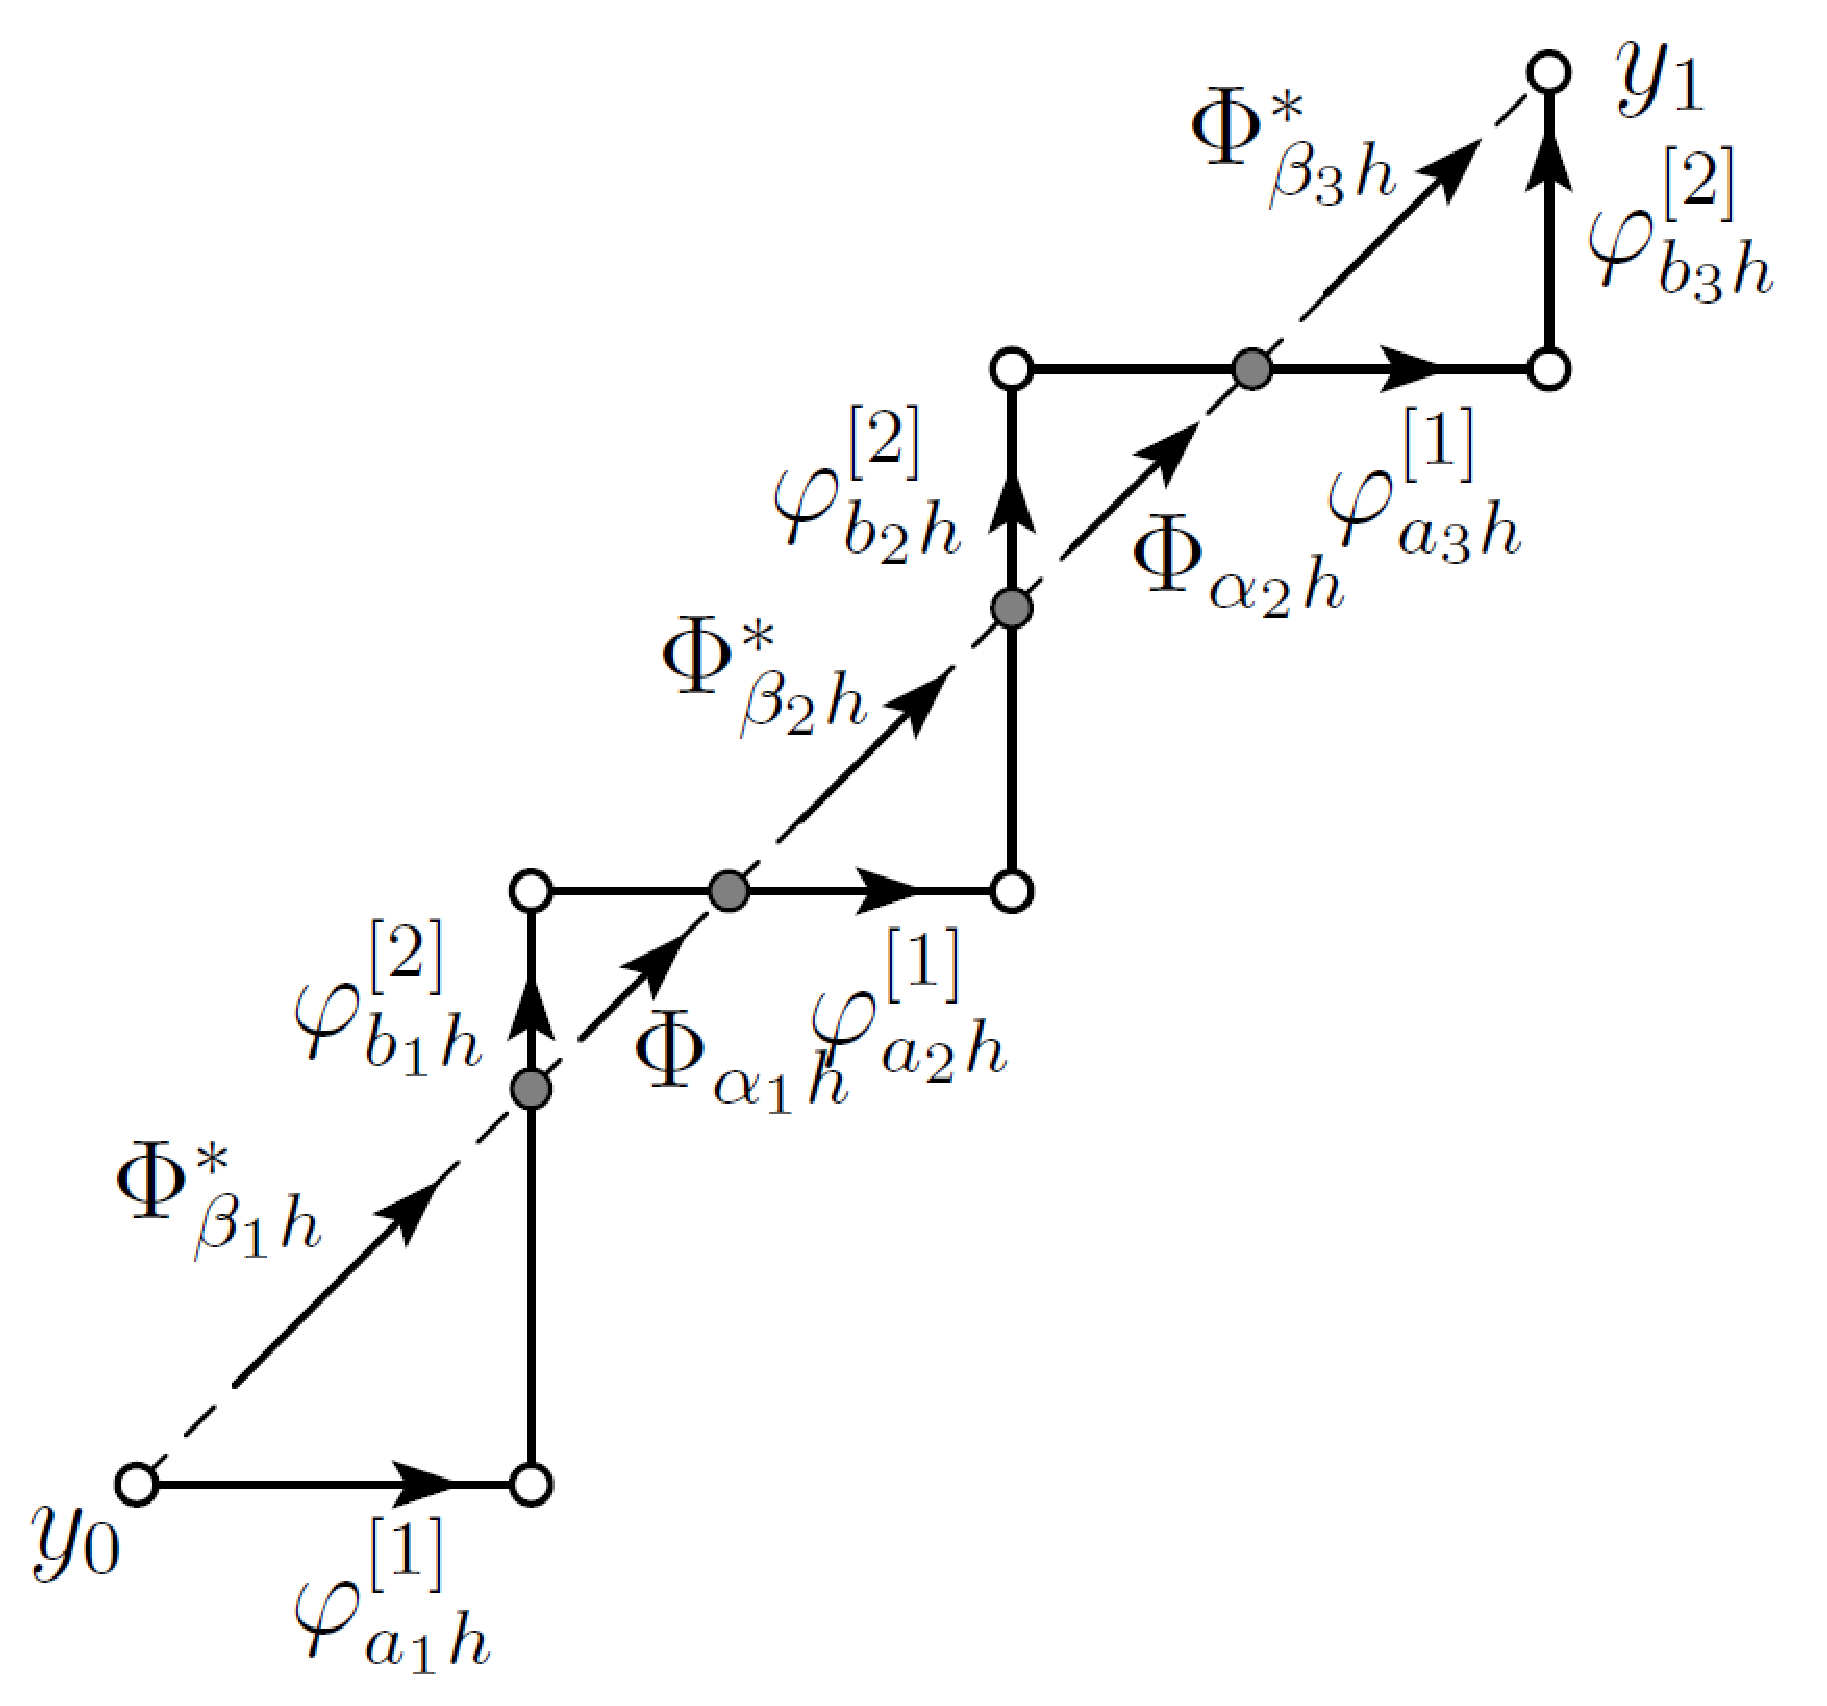
\includegraphics[width=0.45\textwidth]{graphics/split_methods_nstep}
  \caption{For a 2D problem, the propagation of a solution $y$ from an initial value $y_0$ to a postpoint solution $y_1$ is shown over three substeps that amount to a full time step $h$ ($\sum_i \beta_i = \sum_i a_i = 1$). The exact solution is shown generically as the directed diagonal line segment, which records the path of the true solution as accomplished by the exact integrator $\Phi_{\beta_i h}^*$. The composition of split integrators $\varphi_{a_i h}$, each of which individually only convect the solution along one phase space variable while holding the other constant, are shown to approximate the final solution $y_1$. In general, the actual postpoint $\tilde{y}_1$ approximated by the split method is not exactly $y_1$, an error which depends on time. For an $N$th order method for time step $h$, the error is $\mathcal{O}(h^{N+1})$ by our definition.}
  \label{fig:n_step_split_diagram}
\end{figure}


 In fact, we notice these are first order accurate as the above are identical to the Euler method time marching scheme (eqs. \eqref{eq:Euler_x} and \eqref{eq:Euler_v}). In the interest of designing a splitting algorithm that preserves symplecticity, the time evaluation can be staggered such that we interpose symplectic Euler schemes (eqs. \eqref{eq:Symplectic_Euler_x} and \eqref{eq:Symplectic_Euler_v}). Thus, the important realization is made that the Lie (advection) operators $\mathcal{X}^{\tau}$ and $\mathcal{V}^{\tau}$ in a split scheme constitute a first order symplectic Euler scheme over a time step $\tau$. An equivalent statement to \eqref{eq:nth_order_scheme} can then be assembled as the general problem of interleaving symplectic Euler method substeps of fractional time $c_i\tau$ and $d_i\tau$ that sum to a full time step $\tau $ in $k$ stages ($\sum_i c_i \tau = \sum_i d_i \tau = \tau$). Taking $\tau \rightarrow c_i\tau , d_i\tau$, we see from above that the coefficients $c_i$ and $d_i$ enter the integrated characteristics equations:

\begin{eqnarray}
x_i & = & x_{i-1} + c_i \tau v_{i-1} , \qquad\qquad\quad\,\,\,\,  x_k = x(t + \tau) \label{eq:Symplectic_Euler_x_general}\\[0.3em]
v_i & = & v_{i-1} + d_i\tau \left(\frac{q_{\alpha}E(x_i)}{m_{\alpha}}\right), \qquad v_k = v(t + \tau ) \label{eq:Symplectic_Euler_v_general}
\end{eqnarray}

\noindent for each stage $i = 1,2,\ldots , k$, which is a symplectic Euler stepthrough. Thus, rather than expanding exponentials (eq. \eqref{eq:nth_order_scheme}) or otherwise obtaining the coefficients by careful manipulation of the exponential arguments themselves per Yoshida \cite{Yoshida90} by using the Baker-Campbell-Hausdorff formula, the above two equations are straightforwardly matched up to the desired order of accuracy in Taylor series expansion:

\begin{eqnarray*}
x(t + \tau ) & = & x(t) + \tau \dot{x} + \frac{1}{2}\tau^2 \ddot{x} + \ldots \\
&&\\
v(t + \tau ) & = & v(t) + \tau \dot{v} + \frac{1}{2}\tau^2 \ddot{v} + \ldots \\
\end{eqnarray*}

\noindent whereupon physically identifying derivatives, we see that the order conditions take the following forms

\begin{eqnarray}
x(t + \tau ) & = & x(t) + \tau v + \frac{1}{2}\tau^2 \left(\frac{q_{\alpha}E(x)}{m_{\alpha}}\right)_{x = x(t)} + \ldots \label{eq:Taylor_order_conditions_x}\\[1.5em]
v(t + \tau ) & = & v(t) + \tau  \left(\frac{q_{\alpha}E(x)}{m_{\alpha}}\right)_{x = x(t)} + \frac{1}{2}\tau^2 \left(\frac{q_{\alpha}}{m_{\alpha}}\frac{dE}{dt}\right)\biggr|_{x = x(t)} + \ldots \label{eq:Taylor_order_conditions_v}
\end{eqnarray}

To derive the coefficients required for a second order accurate method in time ($n = 2$) two stages of the above scheme are the minimum required ($k \geq 2$). However, it should be noted that split methods are not unique in that multiple schemes with varying stages $k$ can satisfy the same order requirements. This idea is revisited in a moment. Let \ding{172} and \ding{173} denote stages evaluated at times $t_1$ and $t_2$ ($t < t_1 < t_2$ and $t_2 = t + \tau $) for corresponding quantities ($x_1$, $v_1$) and ($x_2$, $v_2$). Applying the advections \eqref{eq:Symplectic_Euler_x_general} and \eqref{eq:Symplectic_Euler_v_general} iteratively, we have the stepthrough from a prepoint $(x,v)$ at time $t$ in phase space to a postpoint $(x_2,v_2)$ at time $t + \tau$

\subsubsection{Stage \ding{172}}

\begin{eqnarray*}
x_1 & = & x +  c_1\tau v  \\[0.3em]
v_1 & = & v + d_1\tau \left(\frac{q_{\alpha}E(x_1)}{m_{\alpha}}\right)  \\[0.3em]
& = & v + d_1\tau \frac{q_{\alpha}}{m_{\alpha}}E(x + c_1\tau v) \\[0.3em]
& = & v + d_1\tau \frac{q_{\alpha}}{m_{\alpha}}\left[E(x) + (c_1\tau v)\frac{\partial E}{\partial x} + \ldots \right] \\[0.3em]
v_1 & = & v + d_1\tau \frac{q_{\alpha}E(x)}{m_{\alpha}} + (c_1d_1\tau^2 )\frac{q_{\alpha}}{m_{\alpha}}\frac{dE}{dt}\biggr|_{x = x(t)} + \ldots
\end{eqnarray*}

\noindent Where we have identified $v (\partial E / \partial x) = (dx/dt)(\partial E / \partial x) = dE/dt$.

\subsubsection{Stage \ding{173}}

\begin{eqnarray}
x_2 & = & x_1 +  c_2\tau v_1 \nonumber \\[0.3em]
& = & (x +  c_1\tau v) + c_2\tau \left[v + d_1\tau \frac{q_{\alpha}E(x)}{m_{\alpha}} + (c_1d_1\tau^2 )\frac{q_{\alpha}}{m_{\alpha}}\frac{dE}{dt}\biggr|_{x = x(t)} + \ldots\right]  \nonumber\\[0.3em]
x(t+\tau ) \equiv x_2 & = & x +  (c_1 + c_2)\tau v + c_2 d_1 \tau^2 \left(\frac{q_{\alpha}E(x)}{m_{\alpha}}\right) + \mathcal{O}(\tau^3) \label{eq:Strang_order_conditions_x}
\end{eqnarray}

\noindent and,

\begin{eqnarray}
v_2 & = & v_1 + d_2\tau \left(\frac{q_{\alpha}E(x_2)}{m_{\alpha}}\right) \nonumber \\[0.3em]
& = & \left[ v + d_1\tau \frac{q_{\alpha}E(x)}{m_{\alpha}} + (c_1d_1\tau^2 )\frac{q_{\alpha}}{m_{\alpha}}\frac{dE}{dt}\biggr|_{x = x(t)} + \ldots \right] + d_2\tau \frac{q_{\alpha}}{m_{\alpha}} E\left(x +  (c_1 + c_2)\tau v + \ldots \right)\nonumber \\[0.3em]
& = & \left[ v + d_1\tau \frac{q_{\alpha}E(x)}{m_{\alpha}} + (c_1d_1\tau^2 )\frac{q_{\alpha}}{m_{\alpha}}\frac{dE}{dt}\biggr|_{x = x(t)} + \ldots \right] + d_2\tau \frac{q_{\alpha}}{m_{\alpha}}\left[E(x) + (c_1 + c_2)\tau v\frac{\partial E}{\partial x}\biggr|_{x = x(t)} + \ldots\right] \nonumber \\[0.3em]
& = & \left[ v + d_1\tau \frac{q_{\alpha}E(x)}{m_{\alpha}} + (c_1d_1\tau^2 )\frac{q_{\alpha}}{m_{\alpha}}\frac{dE}{dt}\biggr|_{x = x(t)} + \ldots \right] + d_2\tau \frac{q_{\alpha}}{m_{\alpha}}\left[E(x) + (c_1 + c_2)\tau \frac{dE}{dt}\biggr|_{x = x(t)} + \ldots \right] \nonumber \\[0.5em]
v(t + \tau ) \equiv v_2 & = & v + (d_1 + d_2)\tau\frac{q_{\alpha}E(x)}{m_{\alpha}} + [c_1(d_1 + d_2) + c_2d_2]\tau^2 \frac{q_{\alpha}}{m_{\alpha}}\frac{dE}{dt}\biggr|_{x = x(t)} + \mathcal{O}(\tau^3) \label{eq:Strang_order_conditions_v}
\end{eqnarray}

\noindent Matching the coefficients in each order of $\tau$ of the compositions and the Taylor expansions gives equations that determine the constants $c_1, c_2, d_1, d_2$. Beginning with the $x$ advection, we compare \eqref{eq:Strang_order_conditions_x} with \eqref{eq:Taylor_order_conditions_x}:

\begin{eqnarray*}
\mathcal{O}(\tau )\, :  & c_1 + c_2 & = 1 \\[0.3em]
\mathcal{O}(\tau^2 ) : & c_2 d_1 & = \frac{1}{2}
\end{eqnarray*}

\noindent Two additional equations are provided by comparing composition \eqref{eq:Strang_order_conditions_v} with Taylor series \eqref{eq:Taylor_order_conditions_v}:

\begin{eqnarray*}
\mathcal{O}(\tau ) \, :  & d_1 + d_2 & = 1 \\[0.3em]
\mathcal{O}(\tau^2 ) : & c_1(d_1 + d_2) + c_2d_2 & = \frac{1}{2}
\end{eqnarray*}

\noindent These order constraints are consistent with the general result for $k \geq n$ stages for $n = 2$ accuracy in time as quoted in \cite[p.263]{Yoshida90}:

\begin{eqnarray*}
c_1 + c_2 + \ldots + c_k & = & 1 \\[0.3em]
d_1 + d_2 + \ldots + d_k & = & 1 \\[0.3em]
c_1(d_1 + d_2 + \ldots + d_k) + c_2(d_1 + d_2 + \ldots + d_k) + c_kd_k & = & \frac{1}{2}
\end{eqnarray*}

A simple solution to the set of simultaneous equations above yield $c_1 = c_2 = 1/2, d_1 = 1, d_2 = 0$. The derivation above only required expanding the electric field to first order accuracy, which is ensured by evaluating the electric field after the first $x$-step, i.e. at $x + v\tau / 2$. Thus, the interleaving in time of two symplectic Euler schemes over a time $t$ to $t + \tau$ amounts to

%momentarily adjust enumerate labeling and indentation
\setlist[enumerate]{leftmargin=16pc}
\setlist[enumerate,1]{label=(\alph*)}

\begin{enumerate}
\item $x(t + \tfrac{\tau}{2})  = x(t) + \frac{1}{2}\tau v(t)$
\item $v(t + \tau )   =  v(t) + \tau\frac{q_{\alpha}E(x)}{m_{\alpha}}\biggr|_{x = x(t + \tau/2)}$
\item $x(t + \tau )  =  x(t + \tfrac{\tau}{2}) + \frac{1}{2}\tau v(t + \tau)$
\end{enumerate}


%reset enumerate environment back to default

\setlist[enumerate]{leftmargin=\parindent}
\setlist[enumerate,1]{label=\arabic*.}

\noindent Or, equivalently in terms of operator notation, the solution to the numerical solution of the Vlasov-Poisson system can be recorded as

$$\boxed{f(t + \tau , x, v) = \mathcal{X}^{\tau /2}_{t + \tau /2}\circ\mathcal{V}^{\tau}_t\circ\mathcal{X}^{\tau / 2}_t f(t,x,v) + \mathcal{O}(\tau^3)} \qquad \qquad \textrm{\underline{Strang splitting}}$$

\noindent Here, a redundant subscript has been introduced to transparently communicate at what time each advection operator begins. As before, the superscript indicates the time step increment. Substituting successively the steps of the scheme just above into the arguments of the distribution function, we see that

 $$f(t+\tau , x, v) = f(t, x - \tau v - \tfrac{1}{2}\tfrac{q_{\alpha}E(\bar{x})}{m_{\alpha}}\tau^2), v - \tfrac{q_{\alpha} E(\bar{x})}{m_{\alpha}}\tau )$$

 \noindent So that,

\begin{eqnarray*}
x(t) & = & x(t + \tau ) - \tau v(t + \tau ) - \tfrac{1}{2}\frac{q_{\alpha}E(t + \tau /2, \bar{x})}{m_{\alpha}}\tau^2 \\
&& \\
v(t) & = & v(t + \tau ) - \frac{q_{\alpha} E(t + \tau / 2, \bar{x})}{m_{\alpha}}\tau
\end{eqnarray*}

\noindent Where the position at half-time step $\bar{x} \equiv x_1 = x + v\tau / 2$. This is a statement of the \emph{Leapfrog}, or \emph{St\"{o}rmer-Verlet}, algorithm. Finally, this composition follows a fortiori from the stronger result that Blanes \cite{Blanes02} reminds us of. That is, the composition of a lower order integrator $\varphi_{\tau}$ with its adjoint $\varphi_{\tau}^{\dagger}$ yields a higher order integrator. For example, recall the first order integrator \eqref{eq:1st_order_scheme}, $\varphi_{\tau ,\mathrm{1st}} \coloneqq \mathcal{X}^{\tau}\circ\mathcal{V}^{\tau}$, that approximates the exact time evolution operator $T^{\tau} = \varphi_{\tau ,\mathrm{1st}} + \mathcal{O}(\tau^2)$. The Strang splitting scheme is reproduced as follows

$$\varphi_{2\tau,\mathrm{2nd}} \equiv \varphi_{\tau ,\mathrm{1st}}\circ\varphi_{\tau ,\mathrm{1st}}^{\dagger} = \mathcal{X}^{\tau}\circ\mathcal{V}^{\tau}\circ\mathcal{V}^{\tau}\circ\mathcal{X}^{\tau} = \mathcal{X}^{\tau}\circ\mathcal{V}^{2\tau}\circ\mathcal{X}^{\tau}$$

\noindent over a time step $2\tau$. Clearly, this is equivalent to

$$T^{\tau} = \varphi_{\tau,\mathrm{2nd}} + \mathcal{O}(\tau^3) =  \mathcal{X}^{\tau /2}_{t + \tau /2}\circ\mathcal{V}^{\tau}_t\circ\mathcal{X}^{\tau / 2}_t + \mathcal{O}(\tau^3) $$

\noindent In turn, this second order integrator can be used as a building block to construct higher order schemes.

\subsection{Higher order integrators}

\indent\indent It is clear from the previous section that while the approach to obtain higher order methods is straightforward, the algebraic burden to obtain even modest orders of accuracy for a minimum number of stages quickly becomes nontrivial. As suggested at the closing of the previous section, a popular method is to compose lower order schemes in order to build higher order integrators. Specifically, \cite{Yoshida90} later put forth that eq. \eqref{eq:nth_order_scheme} is equivalent to

\begin{equation}\prod_{i = 1}^n \exp (c_i\tau \Lambda_x)\exp (d_i\tau \Lambda_v) = \exp (\tau (\Lambda_x + \Lambda_v) + \mathcal{O}(\tau^{n+1})), \qquad \sum_i c_i = \sum_i d_i = 1\label{eq:nth_order_scheme_exp}\end{equation}

\noindent In this way, the Baker-Campbell-Hausdorff (BCH) formula can be applied iteratively, which states for two operators $X = c_1\Lambda_x$, and $Y = d_1\Lambda_v$ for the lowest order method, the exponential product can be written as a single exponential as given by

$$\exp X \exp Y = \exp Z$$

where $Z$ is found to be 

\begin{eqnarray*}
Z & = & X + Y + \frac{1}{2}[X,Y] + \frac{1}{12}([X,[X,Y]] + [Y,[Y,X]]) \\[0.5em]
&&  - \frac{1}{24}[Y,[X,[X,Y]]] - \frac{1}{720}([[[[X,Y],Y],Y],Y] + [[[[Y,X],X],X],X]) + \ldots
\end{eqnarray*}

\noindent and the commutator $[X,Y] = XY - YX$.  To see how higher order methods can be obtained, we consider proving the Strang splitting scheme. Assembling the Strang splitting scheme by composing $\exp X \exp Y \exp X = \exp (\tfrac{1}{2}\tau \Lambda_x) \exp (\tau \Lambda_v) \exp (\tfrac{1}{2}\tau \Lambda_x)$ by iterating on the BCH formula to find $(\exp X \exp Y)\exp X = \exp W$, The argument $W$ is found to be \cite{Yoshida90}:

$$W = \tau \alpha_1 + \tau^3 \alpha_3 + \tau^5 \alpha_5 + \mathcal{O}(\tau^7)$$

\noindent where $\alpha_1 = \Lambda_x + \Lambda_v$, $\alpha_3 = \tfrac{1}{12}[\Lambda_v,[\Lambda_v,\Lambda_x]]$, $\alpha_5 = \tfrac{7}{5760}[\Lambda_x,[\Lambda_x,[\Lambda_x,[\Lambda_x,[\Lambda_v]]]]]$. Thus, truncating the series after the first term assures we are accurate to $\mathcal{O}(\tau^2)$, and the factor of unity in front of the $\alpha_1$ term confirms our splitting coefficients were correct. Alternatively, if we did not know the coefficients a priori, we could have modelled the coefficients as $c_1, c_2$ and $d_1, d_2$ in order expand as above to obtain the necessary order conditions. Higher orders can be obtained by composing additional exponentials and ascertaining the exponential argument by iteration of the BCH formula so that we are able to directly manipulate the arguments of the exponentials alone without the need to expand the exponentials to find and match order conditions. Thus, careful handling of the terms that develop permits extracting the necessary coefficients for a given scheme expediently, where the coefficients are easily computed numerically. Blanes et. al optimized the search for coefficients with respect to a defined error \cite{Blanes02}, giving rise to popular methods used later (O6-4, O11-6).


\chapter{Preliminary work}\label{chap:Preliminary_work}

This chapter presents the research approach and the results accomplished thus far. The aim of this thesis is to develop a computational foundation that furnishes efficient, high order numerical kinetic simulations of edge plasma with self-consistent field calculations in the context of plasmas in the magnetic confinement devices. First, we formally define the discrete advection problem and present the algorithms for the schemes presented in chapter \ref{chap:Literature_review}. We then present results for three schemes: (1) the classic convected scheme (CS), (2) a fifth order accurate method $FD5$ using finite differences to compute the correction terms, and (3) a class of $N$th order accurate CS methods where Fourier transforms are used to calculate the correction terms ($FN$ methods). As a first pass, we confirm they have been implemented properly by verifying their numerical order of accuracy through customary convergence analysis. After, we showcase several test cases including 1D advection with variable velocity, a 2D rotating system to investigate four different splitting schemes (LF2, Y4, O6-4, and O11-6), and finally provide an intermediate test case in handling the 1D-1V Vlasov-Poisson system. That is, the solution to a Vlasov equation is given with a prescribed electric field.


\newpage



\section{The discrete advection problem}\label{sec:The_discrete_problem}

\indent\indent The continuous problem is to seek the solution $f = f(t,x)$ of the hyperbolic partial differential (advection) equation \eqref{eq:Advection} in one dimension subject to a periodic boundary condition:

\vspace{1em}
\fbox{Continuous advection problem}\\[.5em]

\begin{equation}
\frac{\partial f}{\partial t} + v\frac{\partial f}{\partial x} = 0 \label{eq:Advection_1D} , \qquad (x,v)\in\mathcal{M}, \quad t\in\mathbb{R}^+
\end{equation}

\begin{equation}
\textrm{initial condition: } f(0,x) = f_0(x) \qquad x\in [0,L]
\end{equation}

\begin{equation}
\textrm{boundary condition: }f(t,x) = f(t,x+L) \qquad x\in\mathbb{R}
\end{equation}

\noindent where the velocity $v\in\mathbb{R}$ in this test problem is a specified constant so that the continuous problem space is the manifold $\mathcal{M} = \mathbb{R}\times\mathbb{R}$, whereas a particular solution space for a given problem coincides with a line in the two-dimensional tangent bundle $x-v$ at a constant $v$ over the entire real line. The initial distribution $f_0$ is defined over the domain $\mathbb{R}_x = [0,L]$, and is completed over all real numbers $\mathbb{R}$ by the periodicity requirement. Thus, the plasma is both infinite in extent and periodic.

For the discrete problem, at each time $t^n = n\Delta t$ we find a solution $f_h(t^n,x_i,v_j)$ that is an approximation to the exact solution $f(t^n,x_i,v_j)$ for all $(x_i,v_j)\in\mathcal{M}_h$, where the mesh $\mathcal{M}_h$ is the discretization of the manifold $\mathcal{M}$. For this model problem, the mesh (Fig. \ref{fig:Mh_mesh}) is defined in terms of $N_x$ one-dimensional cells $\{C_i\}_{i = 0}^{N_x-1}$ at a constant value $v$ in phase space,

\begin{figure}[h!]
  \centering
    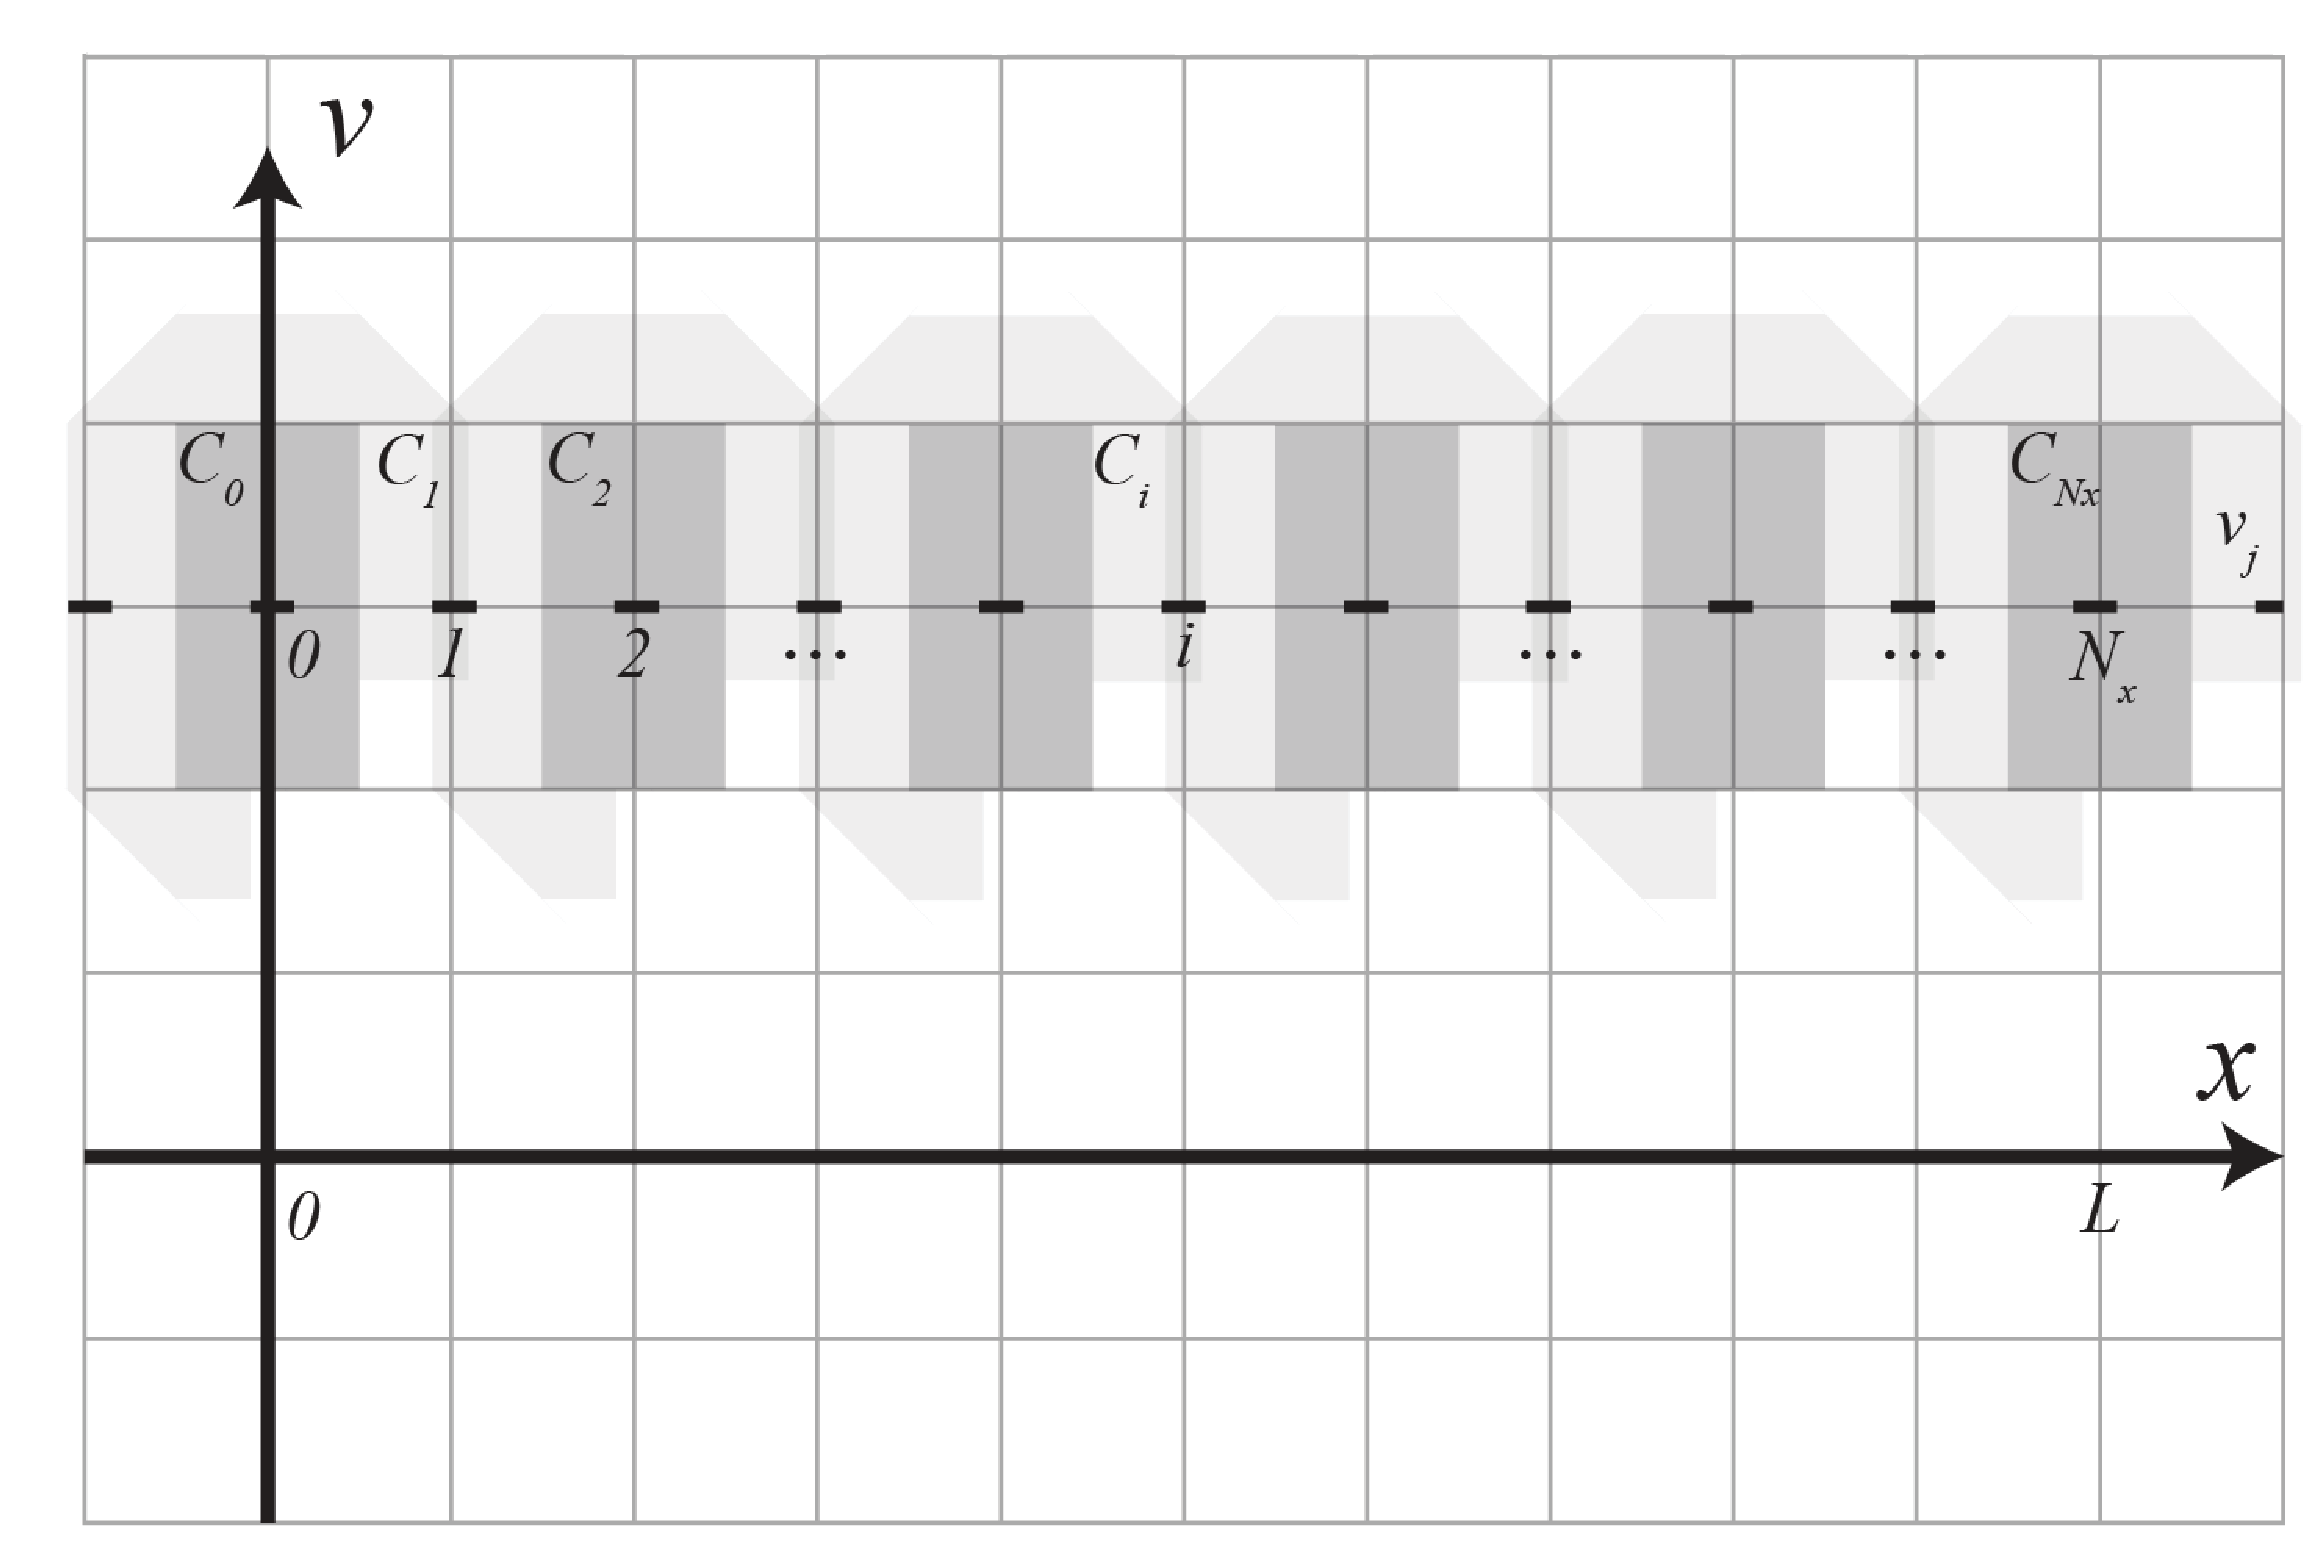
\includegraphics[scale = 0.25]{graphics/Mh_mesh.eps}
  \caption{The mesh $\mathcal{M}_h$ is shown. For the 1D, one-speed, advection case for a periodic plasma, the mesh is a one-dimensional array of cells $C_i$, centered at a constant velocity $v = v_j$. The cells are illustrated as alternating shaded and unshaded objects with a nonzero height for clarity, but it should be noted that in actuality do not have any extent vertically as the velocity is constant.}
  \label{fig:Mh_mesh}
\end{figure}


$$\mathcal{M}_h = \cup_i C_i , \qquad C_j \cap C_k = \varnothing \quad \textrm{for } j \neq k, \qquad i,j,k = 0, 1, \ldots , N_x - 1$$

\noindent Where the cell boundaries are defined at half-distances $x_{i\pm 1/2} = x_i \pm \tfrac{\Delta x}{2}$ whose cell-centers are located at each $\bar{C}_i = x_i$.

 $$C_i = ([x_{i-1/2},x_{i+1/2}],v_j), \qquad x_0 = 0, \, x_{N_x-1} = L$$

\noindent Hence, we always refer to grid points as simple $\{x_i\}$ since their positions do not change with time, whereas convected cell-centers at a time $t^n$ are denoted as $\{x_{i}^n\}$, or sometimes as $\{x_{i'}^n\}$. The widths $\Delta x_i = \Delta x = L / (N_x - 1)$ are chosen to be uniform such that $x_i = x_0 + i\Delta x$ produces the increasing sequence $(x_i)_{i = 0}^{N_x-1}$ that spans a full period $[0,L]$. We complete the sequence over all integers $i\in\mathbb{Z}$ by periodicity, which is most efficiently accomplished using modular arithmetic. In this way, although the system is infinite, all the unique information about its dynamics are contained within a single period $L$, so that numerical simulation is only required over the finite interval $[0,L]$. Thus, the discrete problem is summarized as follows:

\vspace{1em}
\fbox{Discrete advection problem}\\[.5em]

\begin{equation}
\frac{\partial f}{\partial t} + v\frac{\partial f}{\partial x} = 0 \label{eq:Advection_1D} , \qquad (x,v)\in\mathcal{M}, \quad t^n \in (0,T]
\end{equation}

\begin{equation}
\textrm{initial condition: } \quad f(0,x_i) = f_0(x_i),\phantom{_{\mathrm{mod}\, N_x}} \qquad \forall x_i\in [0,L]
\end{equation}

\begin{equation}
\textrm{boundary condition: } f(t^n,x_i) = f(t^n,x_{i\,\mathrm{mod}\, N_x}), \qquad \forall x_i\in\mathbb{R}
\end{equation}

\begin{equation}
i = 0,1,\ldots , N_x-1, \quad \Delta x = \frac{L}{N_x}, \qquad x_i = x_0 + i\Delta x , \, x_0 = 0, \, x_{N_x} = L
\end{equation}

\begin{equation}
n = 0,1,\ldots, N_t, \quad \Delta t = \frac{T}{N_t}, \qquad t^n = n\Delta t , \phantom{x_0 + }\, t^0 = 0, \, t^{N_t} = T 
\end{equation}

\noindent The solution to the discrete problem gives the approximation $f_h(t,x_i) \approx f(t,x_i)$ at the constant $v = v_j$ for all $i$ that exists on the mesh $\mathcal{M}_h$. Henceforth the subscript $h$ is omitted whenever the meaning is clearly understood. Here, we take the centroid values $f_h(t^n,x_i) \equiv f_i^n$.

Defining the rectangle basis function $\mathrm{rect} (z)$, each cell can be used to assemble the approximate solution for the total distribution:\\[1em]


\begin{minipage}{0.4\textwidth}
$$f_h(t^n,x) = \sum_{i\in\mathbb{Z}} f_i^n \, \mathrm{rect}\left(\frac{x - x^n_i}{\Delta x}\right),$$
\end{minipage}
\begin{minipage}{0.4\textwidth}
$$\quad \textrm{where } \mathrm{rect} (z) =
  \begin{cases}
   0 & \text{if } |z| > \tfrac{1}{2} \\[0.3em]
   \tfrac{1}{2} & \text{if } |z| = \tfrac{1}{2}\\[0.3em]
   1 & \text{if } |z| < \tfrac{1}{2}
  \end{cases}
$$
\end{minipage}\\[1em]

\noindent so that each loaded cell has the following form, which we have chosen to have compact support,

$$f_{h,i}(t^n,x) = f_i^n\,\mathrm{rect}\,\left(\frac{x - x^n_i}{\Delta x}\right), \qquad x\in\mathbb{R}$$

The solution is obtained by convecting densities $f^n_{i}$ at time $t^n$ located at prepoints $\{x^n_{i'}\} = \{x_{i}\}$ on the Eulerian grid along characteristics to final positions $\{x_{i'}^{n+1}\}$ over a single time step. The final position of the centroid of a convected cell is generally not coincident with any mesh point $x_{i}$. Density parcels are thus appropriated to cell-centers according to the CS remapping rule (section \ref{subsec:CS_remapping_rule}), which assigns the fraction of density in each MC, $C^{n+1}_{i'}$, to all overlapped cells $\{C_i\}$ in proportion the phase space volume overlap $\zeta^n_{i'\to i}$ assigned for the moving cell whose convection began at time $t^n$. Here, we have simplified the notation of the fraction $\zeta_{i'j'\to ij}$ from section \ref{subsec:CS_remapping_rule} given the velocity $v_j$ is constant in this model problem ($j = j'$), and appended a time label $n$ that marks the start time the convected MC is associated with. In general, this remap fraction is not constant in time nor is it uniform among all cells.

In the 1D case, each MC is remapped to exactly two adjacent cells, $C_i$ and $C_{i\pm 1}$. While the fraction $\zeta^n_{i'\to i}$ can be calculated for each MC relative to every fixed cell $C_i\in\mathcal{M}_h$, we save significant computational cost by calculating a single overlap fraction for a cell $C_i$ for each $C_{i'}$, and use its stored value to deposit the remaining density $1 - \zeta^n_{i'\to i}$ to the other cell $C_{i\pm 1}$. This also proves most natural for hard coding a particle conservation check at each remapping for careful error handling. In this way, we update each cell according to:

\begin{minipage}{0.4\textwidth}
\begin{eqnarray*}
f_i^{n+1} &+\hspace{-.3em}=& \zeta^n_{i'\rightarrow i}f^{n}_{i'} \\[1em]
f_{i\pm 1}^{n+1}&+\hspace{-.3em}=& (1 - \zeta^n_{i'\rightarrow i})\, f_{i'}^{n}
\end{eqnarray*}
\end{minipage}
\begin{minipage}{0.4\textwidth}
$$
    \xymatrix{
       &  & f^{n+1}_i \\
       f^n_{i'} \ar[r]^{T^{\tau}} & f^{n+1}_{i'} \ar[ur]^{\zeta^n_{i'\rightarrow i}} \ar[dr]_{1 - \zeta^n_{i'\rightarrow i}}              & \\
           &                    & f^{n+1}_{i\pm 1} }
$$
\end{minipage}\\[0.3em]


\noindent where the time evolution operator $T^{\tau}$ is shown on the right figure to evolve the solution over a time step (cf. section \ref{subsec:Operator_splitting_theory}). To formalize the computation of the overlap fraction $\zeta^n_{i'\rightarrow i}$, we first note that each cell has constant density in configurational space, so that a moving cell with loaded density $f_{i'}^{n}$ at time $t^n$ that was convected from $x_{i'}^{n}$ to a final location $x_{i'}^{n+1}$ at a time $t^{n+1}$ is represented as

$$f(t^{n+1},x_{i'}) = f_{i'}^{n} \,\mathrm{rect}\left(\frac{x - x_{i'}^{n+1}}{\Delta x}\right)$$

\noindent Then, the fraction of overlap between a cell $C_i$ centered at $x_i$ on the fixed Eulerian grid and the moving cell $C_{i'}$ is given by

\noindent\begin{minipage}{0.55\textwidth}
\quad$$\zeta^n_{i'\to i} = \int \mathrm{rect}\left(\frac{x - x_i}{\Delta x}\right)\mathrm{rect}\left(\frac{x - x^{n+1}_{i'}}{\Delta x}\right)dx = \mathrm{tri}\left(\frac{x_i - x^{n+1}_{i'}}{\Delta x}\right);$$
\end{minipage}
\begin{minipage}{0.45\textwidth}
\begin{equation}\mathrm{tri} (z) =
  \begin{cases}
   1 - |z| & \text{if } |z| < 1 \\[0.3em]
   0 & \text{else }
  \end{cases}
\label{eq:zeta_triangle_function}\end{equation}
\end{minipage}\\[1em]

\noindent where the defined antiderivative of the rectangle function $\mathrm{tri}\,(z) = \int dz\, \mathrm{rect}\,(z)$ is the triangle function.

While the interpretation of the cell overlap is most physical, in practice it is more direct to work with a fraction $\alpha_{i'\to i}^n$ that measures the distance between cell-centers rather than cell boundaries which is the measure that defines $\zeta_{i'\to i}^n$. Thus, it is convenient to not focus on the trajectories themselves, but the overall grid shift that amounts from the convection. In general, the moving cells may be convected by more than one cell spacing $\Delta x$ from their prepoints. By introducing the CFL parameter $\mathcal{C}_{i'}^n$ for the cell $i'$ at a time step beginning at $t^n$, we can decompose the shift into two parts:

\begin{equation}\mathcal{C}_{i'}^n \coloneqq S_{i'}^n + \alpha_{i'\to i}^n, \qquad S_{i'}^n\in\mathbb{Z}, \, \alpha_{i'\to i}^n\in(-1,1)\label{eq:CFL_partition}\end{equation}

$$\textrm{such that } x_{i'}^n \mapsto x_{i'}^{n+1}, \qquad \textrm{where } x_{i'}^{n+1} = [x_{(i'+S_{i'}^n)\,\mathrm{mod}\,N_x} + \alpha_{i'\to i}^n \Delta x]\,\mathrm{mod}\,L$$

\noindent The parameter $S_{i'}^n$ is the integer part of the shift of the moving cell $C_{i'}$ in a single time step that began at time $t^n$ with position $x_{i'}^n \equiv x_{i'}$ on the fixed grid and convected to a location $x_{i'}^{n+1} = x_{(i' + \mathcal{C}_{i'}^n)}$ as defined above on the interval $[0,L]$ per periodic boundary conditions. The fraction $\alpha_{i'\to i}^n$ is the normalized distance between the centroid of the final position of the MC and a nearest neighbor grid point on the fixed mesh $x_{(i'+S_{i'}^n)\,\mathrm{mod}\,N_x}$, which depends on how one chooses to define $S_{i'}^n$ (see below). Again, we have used the convention where the omission of the time value superscript indicates grid points on the fixed mesh.  Introducing the fraction $\alpha_{i'\to i}^n$ removes the need to invoke a triangle function as is used for the calculation of $\zeta_{i'\to i}^n$ (eq. \eqref{eq:zeta_triangle_function}).

There is flexibility in the definition of the two terms in \eqref{eq:CFL_partition}; namely, we can choose the integral shift $S_{i'}^n$ to undershoot (resp. overshoot) the exact final position $(i + \mathcal{C}_{i'}^n)\,\mathrm{mod}\, N_x$, which then fixes the sign of the fraction $\alpha_{i'\to i}^n$ as either positive (resp. negative) for $v \geq 0$ or negative (resp. positive) for $v < 0$. The choice of how these terms are defined, in turn, determines the proportion remapped to each grid point. We choose the general rule that $S_{i'}^n$ and $\alpha_{i'\to i}^n$ have the same sign. Thus, the velocity $v$ and the fraction $\alpha_{i'\to i}^n$ also have the same sign. In physical terms, this amounts to defining the integer shift $S_{i'}^n$ to always undershoot the final location in the direction of convection, so that $\alpha_{i'\to i}^n \geq 0$ (resp. $\alpha_{i'\to i}^n < 0$) when $v \geq 0$ (resp. $v < 0$). Thus,

$$\alpha_{i'\to i}^n = \mathcal{C}_{i'}^n - S_{i'}^n,\qquad \textrm{where } S_{i'}^n = \floor{\mathcal{C}_{i'}^n} \qquad \qquad (v \geq 0)$$

$$\alpha_{i'\to i}^n = \mathcal{C}_{i'}^n - S_{i'}^n,\qquad \textrm{where } S_{i'}^n = \ceil{\mathcal{C}_{i'}^n} \qquad \qquad (v < 0)$$

\noindent Since the CS is a semi-Lagrangian method, its stability is not restricted by the value of the Courant parameter; however, it naturally appears in the stepthrough of the convection process.

Thus, the CS update statement is written as:\\[0.3em]

\underline{Non-uniform $v \geq 0$}
\begin{subequations}
\label{eq:CS_update_increment_version_alpha_i_n_v_positive}
\begin{align}
f_{(i+S_{i'}^n)\,\mathrm{mod}\,N_x}^{n} \,+\hspace{-.3em}=&\,\, (1 - \alpha_{i'\to i}^n )\, f^{n}_{i'} \\[1em]
f_{(i+S_{i'}^n+1)\,\mathrm{mod}\,N_x}^{n}\, +\hspace{-.3em}=& \,\,\alpha_{i'\to i}^n f_{i'}^{n}
\end{align}
\end{subequations}


\underline{Non-uniform $v < 0$}
\begin{subequations}
\label{eq:CS_update_increment_version_alpha_i_n_v_negative}
\begin{align}
f_{(i+S_{i'}^n)\,\mathrm{mod}\,N_x}^{n} \,+\hspace{-.3em}=&\,\,\,\phantom{-}\,(1 + \alpha_{i'\to i}^n )\, f^{n}_{i'} \\[1em]
f_{(i+S_{i'}^n+1)\,\mathrm{mod}\,N_x}^{n}\, +\hspace{-.3em}=& \,\,-\alpha_{i'\to i}^n f_{i'}^{n}
\end{align}
\end{subequations}


\noindent where a complete mesh update amounts to looping over all cells moving cells $C_{i'}$. We note in closing that the unfactored form of the above equations represent an update in terms of normalized ``fluxes'' $\alpha_{i'\to i}^n f_{i'}^n$; a form that will be favored in the following section when higher order corrections are included.

Finally, we specialize the above to the specific case of a uniform constant speed ($v \geq 0$) for the model problem \eqref{eq:Advection_1D}, which is the case at hand. All MCs are convected the same amount $v\Delta t$. Thus, the implementation can be significantly optimized by noting the fractions $\alpha_{i'\to i}^n$ (and, hence $\zeta_{i'\to i}^n$) are constant for all MCs at each time step. It is opportune to compute this single value $\alpha \equiv \alpha_{i'\to i}^n$ at the start, and employ its stored value as needed. The constant speed case will be considered in all schemes with the understanding that no generality is lost given that each MC presents a CS problem with constant speed at each time step.

\subsection{Classic convected scheme algorithm}

 Using the framework developed in section \ref{sec:Classic_convected_scheme}, the implementation for the uniform case is summarized below \emph{\hyperlink{alg:1}{algorithm 1}}. The \\[0.3em]

\phantomsection\hypertarget{alg:1}{}
\noindent\begin{tabular}{l}
\toprule
\textbf{Algorithm 1}: Classic convected scheme solution to the one-speed 1D advection equation \\
\midrule
  \begin{minipage}{\textwidth}
    \vskip 4pt
    \begin{enumerate}
   \item Load cell-centers with densities $\{f^0_{i}\}$ from initial condition for all $i = 0, 1, 2,\ldots, N_x$.
   \item Compute normalized cell displacements $C = \tfrac{v\Delta t}{\Delta x}$ and decompose into integral and fractional parts, $S$ and $\zeta$, respectively
\vskip 1pt
\hspace{3em}$C = S + \alpha, \qquad S\in\mathbb{Z}, \alpha\in [0,1)\subset\mathbb{R}$
\vskip 2pt
where $S = \floor{C}, \quad \alpha = C - S$
   \item Convect density parcels at each $x^n_i \equiv x_{i}$ on the fixed grid by an integral shift $S$ to an intermediate grid point $x^{n}_{i'}$
\vskip 1pt
\hspace{3em}$f(t^{n},x_{i}) \mapsto f(t^{n},x_{i'})$ \qquad $i = 0, 1, 2,\ldots , N_x$
\vskip 2pt
where $x^{n}_{i'} = x_{(i + S)\,\mathrm{mod}\,N_x}$
\item Assign integer-shifted densities $f^{n}_{i'}$ to cell-centers $\{x_i\}$ according to the fraction $\alpha$. For nonnegative velocities, eqs. \eqref{eq:CS_update_increment_version_alpha_i_n_v_positive} provide the update
\vskip 1pt
\hspace{3em} $f_{i'\,\mathrm{mod}\,N_x}^{n+1}\phantom{i_{+ 1)}}\,+\hspace{-.3em}=(1 - \alpha)\,f^{n}_{i'}$ \\[1.5em]
\phantom{space\,\,\,}$f_{(i'+1)\,\mathrm{mod}\,N_x}^{n+1}\,\,\,\,+\hspace{-.3em}= \alpha \, f_{i'}^{n}$
\vskip 2pt
where $i' = (i+S)\,\mathrm{mod}\, N_x$. A similar update is used for negative velocities (eqs. \eqref{eq:CS_update_increment_version_alpha_i_n_v_negative}).
   \end{enumerate}
   \vskip 4pt
 \end{minipage}
 \\
  \hline
 \end{tabular}\\[0.3em]

\subsection{High order convected scheme algorithm}

Regarding the theory developed in section \ref{sec:Higher_order_convected_scheme}, the algorithm with respect to the discrete problem is presented below (section \ref{sec:The_discrete_problem}).\\[0.5em]

\phantomsection\hypertarget{alg:2}{}
\noindent\begin{tabular}{l}
\toprule
\textbf{Algorithm 2}: (General) high order convected scheme solution to the one-speed advection equation \\
\midrule
  \begin{minipage}{\textwidth}
    \vskip 4pt
    \begin{enumerate}
   \item Load cell-centers with densities $\{f^0_{i}\}$ from initial condition for all $i = 0, 1, 2,\ldots, N_x$.
   \item Compute normalized cell displacements $C = \tfrac{v\Delta t}{\Delta x}$ and decompose into integral and fractional parts, $S$ and $\zeta$, respectively
\vskip 1pt
\hspace{3em}$C = S + \alpha, \qquad S\in\mathbb{Z}, \alpha\in [0,1)\subset\mathbb{R}$
\vskip 2pt
where $S = \floor{C}, \quad \alpha = C - S$
   \item Convect density parcels at each $x^n_i \equiv x_{i}$ on the fixed grid by an integral shift $S$ to an intermediate grid point $x^{n}_{i'}$
\vskip 1pt
\hspace{3em}$f(t^{n},x_{i}) \mapsto f(t^{n},x_{i'})$ \qquad $i = 0, 1, 2,\ldots , N_x$
\vskip 2pt
where $x^{n}_{i'} = x_{(i + S)\,\mathrm{mod}\,N_x}$
\item Calculate $N-1$ weighted derivatives coefficients $d_q^n$ required for $N$th order accuracy (e.g. according to \eqref{eq:FD_deriv} for $N = 5$):
\vskip 1pt
\hspace{3em}$\mathlarger{d^n_q = (\Delta x)^q\frac{\partial^q f}{\partial x^q}\biggr|_i^n}$
\vskip 2pt
\item Calculate $N-1$ correction coefficients $c_q$:
\vskip 1pt
\hspace{3em}$\mathlarger{c_q = (-1)^q\beta_q(\alpha)}$
\vskip 2pt
where the functions $\beta_q(\alpha )$ are computed according to \eqref{eq:beta_q}. 
\item Calculate the nominal (normalized) fluxes $\Gamma_i^n$ from eq. \eqref{eq:Uf}, and select corrected flux $[Uf]_i^n$ according to the limiter \eqref{eq:Uf_limiter}:
\vskip 1pt
\hspace{3em}$\mathlarger{\Gamma_i^n = \sum_{q = 0}^{N - 1} c_q d^n_q, \qquad U_i^nf_{i'}^n = \max [\min (0,\Gamma_i^n), f_i^n]}$
\vskip 2pt
\item Assign integer-shifted densities $f^{n}_{i'}$ to cell-centers $\{x_i\}$ according CS remapping rule in flux form:
\vskip 1pt
\hspace{3em} $f_{i'\,\mathrm{mod}\,N_x}^{n+1}\phantom{i_{+ 1)}} \,+\hspace{-.3em}= f_{i'}^n - U_i^nf_{i'}^n$ \\[1.5em]
\phantom{space\,\,\,}$f_{(i'+1)\,\mathrm{mod}\,N_x}^{n+1}\,\,\,\,+\hspace{-.3em}= U_i^nf_{i'}^n$
\vskip 2pt
Where $i' = (i+S)\,\mathrm{mod}\,N_x$. A similiar update is used for negative velocities (eqs. \eqref{eq:CS_update_increment_version_alpha_i_n_v_negative}).
   \end{enumerate}
   \vskip 4pt
 \end{minipage}
 \\
  \hline
 \end{tabular}\\[0.3em]

\noindent To compute the terms $d_q^n$ in \hyperlink{alg:2}{algorithm 2}, any means for numerically calculating the contained derivatives may be employed so long as it matches the desired order conditions of the overall method. The coefficients $d_q^n$ involving derivatives have the form:

$$d_q^n = (\Delta x)^q \frac{\partial f}{\partial x}\biggr|_{i}^n, \qquad q = 1,2, \ldots N - 1$$

\noindent That is, the estimation for an order $N$ method must satisfy:

$$(\Delta x)^q \frac{\partial^q f}{\partial x^q}\biggr|_{i}^n = d_q^n + \mathcal{O}(\Delta x^{N+1})$$

\noindent Since the derivatives are multiplied by a $(\Delta x)^q \, (q \geq 1)$, the numerical approximation of the derivatives has the relaxed constraint on the local truncation error (LTE) for each term:

$$\text{LTE}\,\left(\frac{\partial^q f}{\partial x^q}\biggr|_i^n\right) = \mathcal{O}(\Delta x^{N + 1 - q}), \qquad \text{\underline{Correction criterion on derivative estimates}}$$

\noindent For example, a 5th order method requires a first derivative approximation so that its greatest LTE is of order $(5 + 1 - 1) = 5$, a second derivative estimate requires the error to be no larger than order $(5 + 1 - 2) = 4$, and so on. Thus, the strictest requirement is always on the estimation of the first derivative. Two methods for calculating these derivatives are reviewed below.




\subsection{Finite difference corrections} \label{subsec:FD_implementation}

\indent\indent A central finite difference approximation with a stencil $\{i + r\}$ where $r = \{-2,-1,0,1,2\}$ supplies the following estimates accurate up to the required order for each derivative for an overall 5th order \cite{Fornberg88}:

\begin{subequations}
\label{eq:FD_deriv}
\begin{align}
(\Delta x)\frac{\partial f}{\partial x}\biggr|_i^n & =  \frac{1}{12}f_{i-2}^n - \frac{2}{3}f_{i-1}^n + \frac{2}{3}f_{i+1}^n - \frac{1}{12}f_{i+2}^n + \mathcal{O}(\Delta x^5) \\[0.3em]
(\Delta x)^2\frac{\partial^2 f}{\partial x^2}\biggr|_i^n & =  -\frac{1}{12}f_{i-2}^n + \frac{4}{3}f_{i-1}^n + - \frac{5}{2}f_i^n + \frac{4}{3}f_{i+1}^n - \frac{1}{12}f_{i+2}^n + \mathcal{O}(\Delta x^6) \\[0.3em]
(\Delta x)^3\frac{\partial^3 f}{\partial x^3}\biggr|_i^n & =  -\frac{1}{2}f_{i-2}^n + f_{i-1}^n - f_{i+1}^n + \frac{1}{2}f_{i+2}^n + \mathcal{O}(\Delta x^5) \\[0.3em]
(\Delta x)^4\frac{\partial^4 f}{\partial x^4}\biggr|_i^n & =  f_{i-2}^n -4f_{i-1}^n + 6f_i^n - 4f_{i+1}^n + f_{i+2}^n + \mathcal{O}(\Delta x^6) 
\end{align}
\end{subequations}

So that the overall method calculates a density $f$ with an local truncation error $\mathcal{O}(\Delta x^{5+1})$. In this work, we refer to a method that employs these finite difference (FD) approximations for the derivatives required in the anti-diffusive correction accurate to fifth order as \emph{FD5}. Note, this is equivalent to what G\"{u}\c{c}lu refers to as ``P6'' \cite{Guclu14}. We choose to label in this alternative manner due to the personal preference of the author; this convention is also used in numerical methods literature elsewhere. That is, we refer to an $N$th order method as being correct up to order $\mathcal{O}(\Delta x^N)$ with respect to local truncation error which is the usual definition that appears in (for example) the literature of operating splitting methods, whereas others prefer to define an $N$th order method such that the largest error term is of order $\mathcal{O}(\Delta x^N)$  (e.g. \cite{Guclu14}). 

It is noted by G\"{u}\c{c}lu \cite{Guclu14} and proven in \cite{Fornberg88} that a general recipe for obtaining finite difference coefficients is provided by taking derivatives of the appropriate order Lagrange interpolating polynomial (which is the namesake for G\"{u}\c{c}lu's P6 scheme). Thus, it is at least straightforward to derive higher order versions as needed; however, it quickly becomes computationally expensive (cf. \cite{Shukla05}).

\subsection{Spectral corrections}\label{subsubsec:Spectral_derivatives}

\indent\indent The derivative calculation cost can be reduced as compared to a finite difference estimate by computing the derivatives in Fourier space whereafter an inverse can be taken to recover approximations to the same derivatives in physical space. Using a fast Fourier transform (FFT) algorithm, the number of operations is reduced to $\mathcal{O}(N_x \log_2 N_x)$ per time step.

Conceptually, we expand a function $f(t,x) \equiv f(x)$ in space at a given time $t$ according to the series

$$f(x) = \sum_{k = -\infty}^{\infty} \mathcal{F}[f](k) e^{\text{j}\xi_k x}$$

\noindent where the wave number $\xi_k = 2\pi k / L$, and the time dependence has been suppresed for brevity given we transform the configurational variable $x$. The imaginary unit $\text{j} \coloneqq \sqrt{-1}$ is formatted in plain text to avoid any confusion with the velocity index $j$ previously employed. The choice of this \emph{orthogonal} basis fixes the form of the Fourier coefficients $\mathcal{F}[f](k)$ by consequence; these coefficients are the projections of the density $f(x)$ onto the subspace spanned by each complex exponential basis characterized by the wave number $\xi_k$. The projection is given by the inner product, which is known as the Fourier transform:

$$\mathcal{F}[f](\xi_k) = \frac{1}{L}\int_{-\infty}^{\infty} f(x) e^{-\frac{2\pi\text{j}}{L}kx}dx$$

\noindent To shift to a discrete domain, we choose to center the grid so that the locations in configurational space are represented as $x_m = m\Delta x = m\tfrac{L}{N_x}$, $m = 0, 1, \ldots , N_x - 1$, as is the usual enumeration adopted when invoking Fourier methods given the notational convenience inherited by preserving symmetry. In order to define derivatives consistently, an interpolation is needed between each sample point $x_m$. Minimizing the mean-square slope determines the unique minimium oscillation \emph{trigonometric interpolation} needed which requires the coefficient $\mathcal{F}[f](N_x/2)\, (N_x \, \text{even})$, i.e. the Nyquist term, to be equally split between the positive and negative terms in the series \cite{Johnson11}. The details of this stepthrough in Fourier space are visited in more depth in section \ref{subsubsec:Windowed_Fourier_methods}. The transform pair is approximated in a discrete domain by the discrete Fourier transform (DFT) and inverse discrete Fourier transform (IDFT):

\begin{subequations}
\begin{align}
\mathcal{F}[f](\xi_k) \simeq \text{DFT}[f]_k & \coloneqq  \frac{1}{N_x} \sum_{m = 0}^{N_x - 1} f(x_m) e^{-\text{j}\xi_k x_m} \label{eq:DFT}\\[0.3em] 
f(x_m) \simeq \text{IDFT}[\text{DFT}[f]]_m & \coloneqq  \phantom{\frac{1}{N_x}} \sum_{k = 0}^{N_x - 1}\text{DFT}[f]_k e^{\text{j}\xi_k x_m} \label{eq:IDFT}
\end{align}
\end{subequations}

\noindent Here, the subscripting $k$ and $m$ on the transforms indicate the resulting dependence of the transform (e.g. $\text{DFT}[f]_k$ is a function of $\xi_k = \tfrac{2\pi k}{L}$). In \hyperlink{alg:3}{algorithm 3} below, the transformed terms are referred to as $\{\hat{f}_k\}$. Differentiating the function $f(x_m)$ in the definition \eqref{eq:IDFT} above, we see that differentiation is equivalent to complex multiplication operations in Fourier space,



$$\frac{d^qf}{dx^q}\biggr|_{x = x_m}  \simeq  \frac{1}{N_x} \sum_{k = 0}^{N_x - 1}(\text{j}\xi_k)^q\text{DFT}[f]_k e^{\text{j}\xi_k x_m} = \text{IDFT}\{(\text{j}\xi_k)^q\text{DFT}[f]_k\}$$

\noindent Each transform requires $\mathcal{O}(N_x^2)$ operations. Choosing to use a fast Fourier transform (FFT) and its corresponding inverse (IFFT), the transforms can be reduced to $\mathcal{O}(N_x\log_2 N_x)$ complexity. Thus, an FFT/IFFT prodedure can be substituted above in order to calculate each derivative as needed according to:

\begin{equation}
\boxed{\frac{d^qf}{dx^q}\biggr|_{x = x_m}  \simeq \text{IFFT}\{(\text{j}\xi_k)^q\text{FFT}[f]_k\}} \qquad \text{where } \xi_k = \frac{2\pi k}{L}, k = 0, 1, \ldots, N_x - 1 \label{eq:FFT_deriv}
\end{equation}
 
\noindent Because of the distinct procedure involved in the spectral calculation, a dedicated algorithm is presented below so that the particulars are clear. We refer to this method as \emph{spectral-CS}, and identify an $N$th order method that calculates derivatives in Fourier space as above, as an $FN$ algorithm. For example, a 15th order method is called \emph{F15}. Note, that a low-pass filter is used to zero out any Fourier coefficients that contribute insignificantly on their own, but whose usually high frequency (especially amplified at higher powers) presents a source of white noise.\\[0.3em]

\phantomsection\hypertarget{alg:3}{}
\noindent\begin{tabular}{l}
\toprule
\textbf{Algorithm 3}: (Spectral derivatives) high order convected scheme solution to the one-speed advection equation \\
\midrule
  \begin{minipage}{\textwidth}
    \vskip 4pt
    \begin{enumerate}
   \item Load cell-centers with densities $\{f^0_{i}\}$ from initial condition for all $i = 0, 1, 2,\ldots, N_x$.
   \item Compute normalized cell displacements $C = \tfrac{v\Delta t}{\Delta x}$ and decompose into integral and fractional parts, $S$ and $\zeta$, respectively
\vskip 1pt
\hspace{3em}$C = S + \alpha, \qquad S\in\mathbb{Z}, \alpha\in [0,1)\subset\mathbb{R}$
\vskip 2pt
where $S = \floor{C}, \quad \alpha = C - S$
   \item Convect density parcels at each $x^n_i \equiv x_{i}$ on the fixed grid by an integral shift $S$ to an intermediate grid point $x^{n}_{i'}$
\vskip 1pt
\hspace{3em}$f(t^{n},x_{i}) \mapsto f(t^{n},x_{i'})$ \qquad $i = 0, 1, 2,\ldots , N_x$
\vskip 2pt
where $x^{n}_{i'} = x_{(i + S)\,\mathrm{mod}\,N_x}$
\item Calculate the Fourier transform $\hat{f}^n_k$ of the density $f_i^n$ via a fast Fourier transform (FFT) algorithm:
\vskip 1pt
\hspace{3em} $\hat{f}_k = \text{FFT}[f], \qquad \text{if } |\hat{f}_k| \leq A\varepsilon , \text{then set} \hat{f}_k^n = 0$
\vskip 2pt
where $\varepsilon = 2\times 10^{-15}$ and $A = \max_k |\hat{f}_k^n|)$.
\item Calculate the associated wave numbers $\xi_k$:
\vskip 1pt
\hspace{3em}$ \xi_k =
  \begin{cases}
   2\pi k / L & \text{if } k \leq N_x/2 \\[0.5em]
   2\pi (k - N_x) / L       & \text{else}
  \end{cases}$
\vskip 2pt
\item Calculate the $N-1$ derivative coefficients $\hat{d}_q^n$ in Fourier space required for the desired order of accuracy $N$. 
\vskip 1pt
\hspace{3em} $\hat{d}_q^n = (\text{j}\xi_k)^q \hat{f}_k, \qquad q = 0,1,\ldots , N - 1$
\vskip 2pt
\item Calculate $N-1$ correction coefficients $c_q$:
\vskip 1pt
\hspace{3em}$c_q = (-1)^q \beta_q(\alpha )$
\vskip 2pt
where the functions $\beta_q(\alpha )$ are computed according to \eqref{eq:beta_q}. 
\item Calculate the nominal (normalized) fluxes $\hat{\Gamma}_i^n$ by assembling the equivalent of eq. \eqref{eq:Uf}
\vskip 1pt
\hspace{3em}$\mathlarger{\hat{\Gamma}_i^n = \sum_{q = 0}^{N - 1} c_q \hat{d}^n_q}$
\vskip 2pt
\item Calculate the flux in configurational space by applying an inverse fast Fourier transforom (IFFT), and select corrected flux $[Uf]_i^n$ according to the limiter \eqref{eq:Uf_limiter}:
\vskip 1pt
\hspace{3em}$\Gamma_i^n = \text{Re }[\,\text{IFFT}\{\hat{\Gamma}_i^n\}], \qquad U_i^nf_{i'}^n = \max [\min (0,\Gamma_i^n), f_i^n]$
\vskip 2pt
where the real part is applied to remove any residual (negligibly small) imaginary component artifacts that can result from the IFFT process.
\item Assign integer-shifted densities $f^{n}_{i'}$ to cell-centers $\{x_i\}$ according CS remapping rule in flux form:
\vskip 1pt
\hspace{3em} $f_{i'\,\mathrm{mod}\,N_x}^{n+1}\phantom{i_{+ 1)}} \,+\hspace{-.3em}= f_{i'}^n - U_i^nf_{i'}^n$ \\[1.5em]
\phantom{space\,\,\,}$f_{(i'+1)\,\mathrm{mod}\,N_x}^{n+1}\,\,\,\,+\hspace{-.3em}= U_i^nf_{i'}^n$
\vskip 2pt
Where $i' = (i+S)\,\mathrm{mod}\,N_x$. A similiar update is used for negative velocities (eqs. \eqref{eq:CS_update_increment_version_alpha_i_n_v_negative}).
   \end{enumerate}
   \vskip 4pt
 \end{minipage}
 \\
  \hline
 \end{tabular}\\



\section{Results}\label{sec:Results}

\indent\indent For all simulations, we solve an advection equation with unit velocity ($v = 1$)

\begin{subequations}
\label{eq:Advec_eq_1D_unit_vel}
\begin{align}
\frac{\partial f}{\partial t} + \frac{\partial f}{\partial x} = 0, &\qquad x\in\mathcal{D}, t\in [0,T] \label{eq:advec_equation_unit_vel}\\[1em]
f(0,x) = f_0(x), & \quad f(t,x + L) = f(t,x)
\end{align}
\end{subequations}

\noindent where the domain $\mathcal{D}$ and time duration $T$ depends on the test case at hand. The initial distributions $f_0(x)$ are chosen to prove numerical order of accuracy, and thereafter we investigate test cases that challenge the fidelity of each scheme's calculations in telling situations. The boundary condition is, as usual, periodicity (cf. section \ref{sec:The_discrete_problem}). As described in the previous section, a mesh refinement exercise is conducted by holding the Courant-Friedrichs-Lewy (CFL) parameter $\mathcal{C}$ constant while increasing the resolution of the grid consistently. The problem can be set up so that this amounts to maintaining a simple relationship between the grid points $N_x$ and $N_t$ for a given simulation. Here, the time $T$ and domain length $L$ are decided so that a full simulation covers the advection of a density over a full domain length $L$ in time $T$ (i.e. $L / T = 1$). The CFL parameter for this unit velocity case is then given by: $\mathcal{C} = \tfrac{v\Delta t}{\Delta x} = \tfrac{1\cdot N_t / T}{N_x / L} =  \tfrac{N_x}{N_t}$. The value $\mathcal{C} = 0.32$ is selected so that any combination of $N_x = 8r, N_t = 25r$ for $r\in\mathbb{N}^+$ is permissible for each simulation. However, we note that $N_x$ should be chosen as a power of 2 for spectral CS cases in order to take full advantage of the treecode algorithm on which all FFT procedures are based.

%and compare numerical solutions computed according to classic convected scheme (CS), 5th order accurate corrected CS using finite difference derivative estimations (FD5), and a spectral-CS method correct to order 21 (F21). The spectral method is the motivating reason for initially considering this smooth periodic case, as this removes any any source of Gibbs oscillation (e.g. as occur in the Fourier approximation of functions near sharp edges) which would restrict the extent that we may juxtapose one scheme to another. We use this test case to verify the order of accuracy of each method.

\subsection{Verifying numerical order of accuracy}

\indent\indent We choose to define an $N$th order method when the local truncation error (LTE) is $\mathcal{O}(\Delta x^{N+1})$ (i.e. the numerical approximation is said to be $N$th order accurate). To ensure the method has been implemented correctly, an error calculation of the simulation results for test cases where the exact solution is known can be straightforwardly computed. For the one-speed advection equations, the exact solution $f$ is given by the method of characteristics as $f(t^n,x_i) = f_0(x_i - n\Delta t)$, where $f_0$ is the initial distribution so that the initial condition can be used to directly calculate values of the exact solution for any position and time. A standard measure of the error is the \emph{global error} (GE), which is the error accumulated over a full simulation time $T = N_t \Delta t$, where $N_t$ is the total number of time steps and $\Delta t$ is the associated time step. Formal treatments of the error involved in semi-Lagrangian schemes and the conditions for convergence are provided by a series of papers by Besse et. al (e.g. \cite{Besse08}). The same order result can be obtained less rigorously by understanding the error over $N_t$ time steps for an $N$th order method whose LTE is by definition $\mathcal{O}(\Delta x^{N+1})$ is given by the accumulated error $N_t\cdot \mathcal{O}(\Delta x^{N+1}) = \tfrac{T}{\Delta t}\,\mathcal{O}(\Delta x^{N+1}) = \mathcal{O}(\Delta x^{N+1} / \Delta t)$, where the asymptotic behavior of the spatial and time error depend on how one is related to the other. 

It is common practice to hold, say, $\Delta t$ constant and to refine the mesh $\Delta x$ in successive simulations in order to map the converged error on a logarithmic plot or otherwise provide a direct order calculation. For several numerical methods, the stability of the method asserts an upper limit on the Courant-Friedrichs-Lewy (CFL) parameter $\mathcal{C} \coloneqq \tfrac{v\Delta t}{\Delta x}$, where $v$ is a specified constant that characterizes the problem. While semi-Lagrangian methods have no CFL restriction; however, we note that they are unique in that there is zero error associated with convecting cells an integral number of cells, i.e. whenever $\mathcal{C}\in\mathbb{Z}$.  Thus, following the prescription in a semi-Lagrangian scheme produces errors that vary nonmonotonically with the grid spacing $\Delta x$ since the error dips to zero when $\mathcal{C}$ is an integer. Notwithstanding, the error of the scheme is still present as the enveloping curve that traces the upper bound of the error. Here, we choose instead to fix the CFL parameter between successive simulations so that by its definition $\mathcal{C}\Delta x = v\Delta t$, and the orders are simply related: $\mathcal{O}(\Delta t) = \mathcal{O}(\Delta x)$. Thus, the global error result above is $\mathcal{O}(\Delta x^{N+1} / \Delta t) = \mathcal{O}(\Delta x^{N+1} / \Delta x) = \mathcal{O}(\Delta x^N)$. \emph{For an order $N$ method, we thus will observe a global error (GE) of $\mathcal{O}(\Delta x^N)$ which is associated with a local truncation error (LTE) of $\mathcal{O}(\Delta x^{N+1})$}. 

To gauge a measure of the global error, we choose to work with the standard deviation of the numerical solution to the convected scheme $f_{_{\mathrm{CS}}}(t^n,x_i)$ relative to the exact solution $f_{_{\mathrm{exact}}}(t^n,x_i)$, whereafter an average value is recorded by dividing over the length of the spatial domain. Such an error measure is otherwise known as the \emph{standard error} in statistics. In estimation theory, we regard the estimator $\hat{\theta}$ as the numerical solution $f_{_{\mathrm{CS}}}(t^n,x_i)$ ($\hat{\theta} \equiv f_{_{\mathrm{CS}}}(t^n,x_i)$) and the observable $\theta \equiv f_{_{\mathrm{exact}}}(t^n,x_i)$, so that \emph{normalized root-mean-square error} (NRMSE) is given by $\text{NRMSE}\, = \sqrt{\mathbb{E}[(\theta - \hat{\theta})^2] / L}$ where $L$ is the domain length. That is, we have elected to use the $L^2$ norm as an appropriate measure of the distance between solution and estimator given the solution exists in the Sobolev space $W^{k,p}$, where $W^{k,p} \supset W^{k,2}$ contains the Banach space that is Lebesgue integrable under the 2-norm so that our calculations are guaranteed to be finite and bounded.


Thus, the NRMS of the local truncation error ($\overline{\text{LTE}}_{\Delta x}^n$) of a simulation with mesh spacing $\Delta x$ can be calculated at a particular time step $t^n$ as:

$$\overline{\text{LTE}}^n_{\Delta x} = \left[\frac{\mathlarger{\sum}\limits_{i = 0}^{N_x - 1} [f_{_{\mathrm{CS}}}(t^n,x_i) - f_{_{\mathrm{exact}}}(t^n,x_i)]^2\Delta x}{\mathlarger{\sum}\limits_{i = 0}^{N_x-1} \,\Delta x}\right]^{1/2} = \frac{1}{\sqrt{L}}\left[\sum\limits_{i = 0}^{N_x - 1} [f_{_{\mathrm{CS}}}(t^n,x_i) - f_{_{\mathrm{exact}}}(t^n,x_i)]^2\Delta x\right]^{1/2}$$

\noindent where it is recognized that the sum in the denominator is equal to the length of the domain $L$. For an $N$th order method, this measure will produce an error of $\mathcal{O}(\Delta x^{N+1})$. Similarly, the NRMS of the global error ($\overline{\text{GE}}_{\Delta x}$) is found by evaluating the above at the simulation completion time $t^{N_t} = T$

\begin{equation}
\label{eq:GE}
\overline{\text{GE}}_{\Delta x} = \frac{1}{\sqrt{L}}\left[\sum\limits_{i = 0}^{N_x - 1} [f_{_{\mathrm{CS}}}(T,x_i) - f_{_{\mathrm{exact}}}(T,x_i)]^2\Delta x\right]^{1/2}
\end{equation}

\noindent For an $N$th order method, this error should be on the order $\mathcal{O}(\Delta x^N)$. In order to calculate the order directly, we consider two successive simulations over the same time interval $[0,T]$ where one mesh size $\Delta x$ (and $N_x$ grid points) is twice as large as the other $\Delta x / 2$ (and $2N_x$ grid points). The numerical order observed can be seen as extractable of the ratio of these two global errors:

$$\frac{\overline{\text{GE}}_{\Delta x\phantom{/2}}}{\overline{\text{GE}}_{\Delta x / 2}}  =   \frac{\mathlarger{\frac{1}{\sqrt{L}}}\left[\mathlarger{\sum}\limits_{i = 0}^{N_x - 1} [f_{_{\mathrm{CS}}}(T,x_i) - f_{_{\mathrm{exact}}}(T,x_i)]^2\Delta x\right]^{1/2}}{\mathlarger{\frac{1}{\sqrt{L}}}\left[\mathlarger{\sum}\limits_{i = 0}^{N_x - 1} [f_{_{\mathrm{CS}}}(T,x_i) - f_{_{\mathrm{exact}}}(T,x_i)]^2\,\mathlarger{\frac{\Delta x}{2}}\right]^{1/2}}  = \frac{\left[\mathlarger{\sum}\limits_{i = 0}^{N_x - 1} [f_{_{\mathrm{CS}}}(T,x_i) - f_{_{\mathrm{exact}}}(T,x_i)]^2\right]^{1/2}}{\left[\mathlarger{\sum}\limits_{i = 0}^{N_x - 1} [f_{_{\mathrm{CS}}}(T,x_i) - f_{_{\mathrm{exact}}}(T,x_i)]^2\,\left(\mathlarger{\frac{1}{2}}\right)\right]^{1/2}}$$


\noindent Noting that we are evaluating the final time $t^{N_t} = T$, we understand that the error terms are of order $\mathcal{O}(\Delta x^N)$ from the discussion just above. That is, there exists a constant $C$, independent of mesh size $\Delta x$, such that $|f_{_{\mathrm{CS}}}(T,x_i) - f_{_{\mathrm{exact}}}(T,x_i)| \leq C\Delta x^N$. Or, an equality can be asserted such that $|f_{_{\mathrm{CS}}}(T,x_i) - f_{_{\mathrm{exact}}}(T,x_i)| =  C\Delta x^N + \mathcal{O}(\Delta x^{N+1})$. Lastly, noting that the effect of each sum amounts to multiplying the bounded squared error term by the number of grid points ($N_x$ or $2N_x$), we can write:

\begin{eqnarray*}
\frac{\overline{\text{GE}}_{\Delta x\phantom{/2}}}{\overline{\text{GE}}_{\Delta x / 2}} & = & \left\{\frac{N_x[C\Delta x^N + \mathcal{O}(\Delta x^{N+1})]^2}{(2N_x)[C\left(\frac{\Delta x}{2}\right)^N + \mathcal{O}\left(\frac{\Delta x}{2}\right)^{N+1}]^{^2}\left(\frac{1}{2}\right)}\right\}^{1/2} \\[0.5em]
 & = & \left\{\frac{[C\Delta x^N + \mathcal{O}(\Delta x^{N+1})]^2}{[C\left(\frac{\Delta x}{2}\right)^N + \mathcal{O}\left(\frac{\Delta x}{2}\right)^{N+1}]^{^2}}\right\}^{1/2} \\[0.5em]
 & = & \phantom{2^N}\left|\frac{C\Delta x^N + \mathcal{O}(\Delta x^{N+1})}{C\left(\frac{\Delta x}{2}\right)^N + \mathcal{O}\left(\frac{\Delta x}{2}\right)^{N+1}}\right| \\[0.5em]
 & = & 2^N \frac{C\Delta x^N + \mathcal{O}(\Delta x^{N+1})}{C\Delta x^N + \tfrac{1}{2}\mathcal{O}(\Delta x^{N+1})}, \qquad (C > 0) \\[0.5em]
 & = & 2^N \left(\frac{C\Delta x^N + \tfrac{1}{2}\mathcal{O}(\Delta x^{N+1})}{C\Delta x^N + \tfrac{1}{2}\mathcal{O}(\Delta x^{N+1})} + \frac{\tfrac{1}{2}\mathcal{O}(\Delta x^{N+1})}{C\Delta x^N + \tfrac{1}{2}\mathcal{O}(\Delta x^{N+1})}\right)\\[0.5em]
 & = & 2^N\left(1  +  \frac{\tfrac{1}{2}\mathcal{O}(\Delta x^{N+1})}{C\Delta x^N + \tfrac{1}{2}\mathcal{O}(\Delta x^{N+1})}\right)\\[0.5em]
\frac{\overline{\text{GE}}_{\Delta x\phantom{/2}}}{\overline{\text{GE}}_{\Delta x / 2}} & = & 2^N\left(1  +  \frac{\mathcal{O}(\Delta x)}{2C + \mathcal{O}(\Delta x)}\right)\\
\end{eqnarray*}

\noindent In practice, we can refine the mesh so that $\Delta x$ gets smaller and smaller ($\Delta x \rightarrow 0$). For $\mathcal{O}(\Delta x) \ll 1$, we have $\tfrac{\mathcal{O}(\Delta x)}{2C} \lll 1$, ($C > 0$) so that the above fraction can be properly expanded:

$$\frac{\mathcal{O}(\Delta x)}{2C + \mathcal{O}(\Delta x)} = \frac{\mathcal{O}(\Delta x)}{2C}\left[1 + \frac{\mathcal{O}(\Delta x)}{2C} + \frac{1}{2}\left(\frac{\mathcal{O}(\Delta x)}{2C}\right)^2 + \ldots \right] \simeq \frac{\mathcal{O}(\Delta x)}{2C} = \mathcal{O}(\Delta x)$$

\noindent So the ratio of NRMS global errors give the estimate in the limit of decreasing mesh spacing $\Delta x$:

$$\frac{\overline{\text{GE}}_{\Delta x\phantom{/2}}}{\overline{\text{GE}}_{\Delta x / 2}}  =  2^N(1 + \mathcal{O}(\Delta x))$$

\noindent Thus, it can be seen that operating with the base-2 logarithm recovers the numerical order of accuracy:

\begin{eqnarray*}
\log_2 \frac{\overline{\text{GE}}_{\Delta x\phantom{/2}}}{\overline{\text{GE}}_{\Delta x / 2}} &  = &  \log_2 2^N(1 + \mathcal{O}(\Delta x)) \\
 &  = &  \log_2 2^N + \log_2 (1 + \mathcal{O}(\Delta x)) \\
 &  = &  N + (\mathcal{O}(\Delta x) - \frac{1}{2}(\mathcal{O}(\Delta x))^2 + \frac{1}{3}(\mathcal{O}(\Delta x))^3 + \ldots) \\
\log_2 \frac{\overline{\text{GE}}_{\Delta x\phantom{/2}}}{\overline{\text{GE}}_{\Delta x / 2}} & = & N + \mathcal{O}(\Delta x)
\end{eqnarray*}

\noindent where the smallness of the parameter $\mathcal{O}(\Delta x) \ll 1$ has been exploited again to expand the logarithm. Thus, we see that in the limit of decreasing mesh spacing $\Delta x \rightarrow 0$, this computation exactly recovers the observed order of accuracy in the numerical simulation:

\begin{equation}
\label{eq:Order}
\boxed{N \coloneqq \log_2 \left(\frac{\overline{\text{GE}}_{\Delta x\phantom{/ 2}}}{\overline{\text{GE}}_{\Delta x / 2}} \right), \quad \Delta x \rightarrow 0} \qquad \underline{\text{Observed order of accuracy}}
\end{equation}

\noindent In practice, we perform a mesh refinement series where the same simulation is run for spacings $\Delta x$ halved from one simulation to the next. This order computation approaches a value when the spacing $\Delta x$ reaches sufficiently small values.

\subsubsection{Convergence results}

To demonstrate that the classic CS has been implemented properly, we consider a smoothly varying initial distributionand prescribe a domain of two full periods over a time interval $0 \leq t \leq 2\pi$:

\begin{equation}f_0(x) = 1.1 + \cos(2x), \qquad x\in\mathcal{D} = [-\pi, \pi], \quad t\in [0,2\pi], \quad \text{domain length } L = 2\pi \label{eq:cosine_2x}\end{equation}

\noindent The results are summarized in table \ref{tbl:ClassicCS_order_cos2x}, and one case of a numerical solution taken at the end of the simulation time is shown in figure \ref{fig:ClassicCS_cos2x}.

\begin{table}
\centering
\makebox[0pt][c]{\parbox{1.1\textwidth}{%
\qquad\begin{minipage}{0.35\hsize}
\centering
\ra{1.3}\captionsetup{width=7cm}
\begin{tabular}{@{}llll@{}}\toprule
&\multicolumn{3}{c}{\phantom{$^2$ glob }Classic CS} \phantom{Ordera}\\
\cmidrule{2-4}& $\text{NRMS}(\text{GE}_{\Delta x})$ & Order \\ \midrule
$\phantom{a}N_x$\\
$\phantom{a}32$ & $1.4448\phantom{\times 10^{-1}}$ & $-$ \\
$\phantom{a}64$ & $1.0073\phantom{\times 10^{-1}}$ & 0.5204 \\
$\phantom{a}128$ & $6.0739\times 10^{-1}$ & 0.7298 \\
$\phantom{a}256$ & $3.3537\times 10^{-1}$ & 0.8569 \\
$\phantom{a}512$ & $1.7646\times 10^{-1}$ & 0.9264  \\
$\phantom{a}1024$ & $9.0539\times 10^{-2}$ & 0.9626 \\
$\phantom{a}2048$ & $4.5863\times 10^{-2}$ & \textcolor{red}{0.9812} \\
\bottomrule
\end{tabular}
\captionof{table}{Mesh refinement results for the classic convected scheme applied to the density \eqref{eq:cosine_2x}. The normalized root mean square (NRMS) of the global error (GE) for each mesh with spacing $\Delta x = L/N_x$ is given by eq. \eqref{eq:GE}, and the observed numerical order of accuracy is computed per \eqref{eq:Order}. The CFL number $\mathcal{C} = 0.32$ for all simulations. The numerical order is converging towards $\mathcal{O}(\Delta x^1)$.}
\label{tbl:ClassicCS_order_cos2x}
\end{minipage}
\hfill
\begin{minipage}{0.65\hsize}
\centering
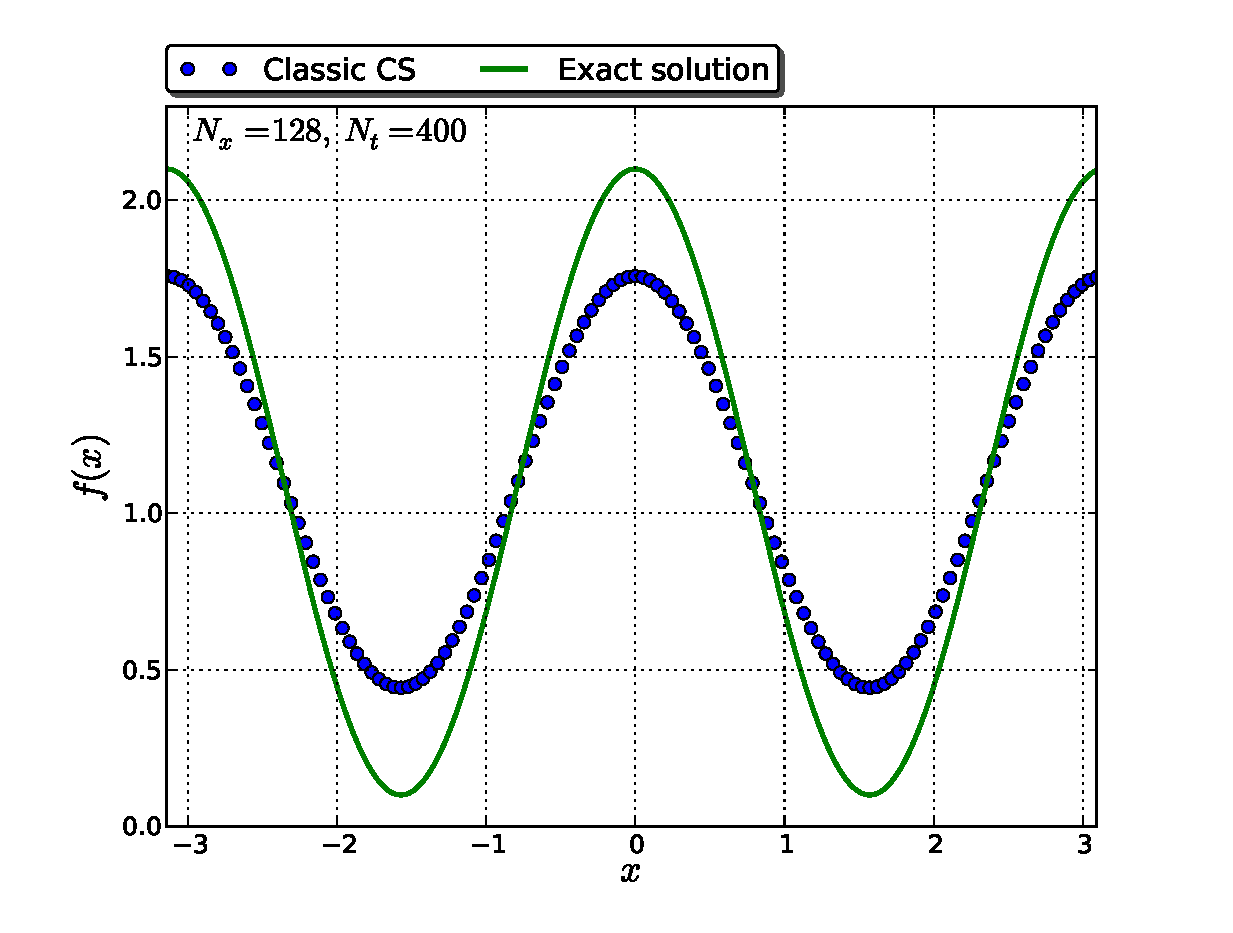
\includegraphics[width=\hsize]{graphics/plot_-_cos2x_ClassicCS__Nx128Nt400_w_f0_itmax.eps}
\captionsetup{width=0.75\hsize}  \captionof{figure}{A classic CS solution after $N_t = 400$ time steps of eq. \eqref{eq:Advec_eq_1D_unit_vel} for $f_0$ given by \eqref{eq:cosine_2x}.}
 \label{fig:ClassicCS_cos2x}
\end{minipage}
}}
\end{table}

It is seen that numerical diffusion contaminates the results and acts to artificially flatten the distribution over time. The effect is most pronounced in coarse grids where the remapping rule appropriates density over larger spatial extents (see figure \ref{fig:ClassicCS_cos2x_several_cases}). In this present case of a slowly varying density, this consequence is modest given the lack of fine structure that needs to be retained along many remap stages. Thus, this cosine distribution \eqref{eq:cosine_2x} permits the early suggestion that the order of accuracy is converging towards $\mathcal{O}(\Delta x^1)$, as is known from theory about semi-Lagrangian methods such as the CS \cite{Besse08} (i.e. the error is $\mathcal{O}(\Delta x^2)$). calculation at relatively coarse mesh sizes ($N_x \sim 1024$, table \ref{tbl:ClassicCS_order_cos2x}).

\begin{figure}[h!]
 \centering
   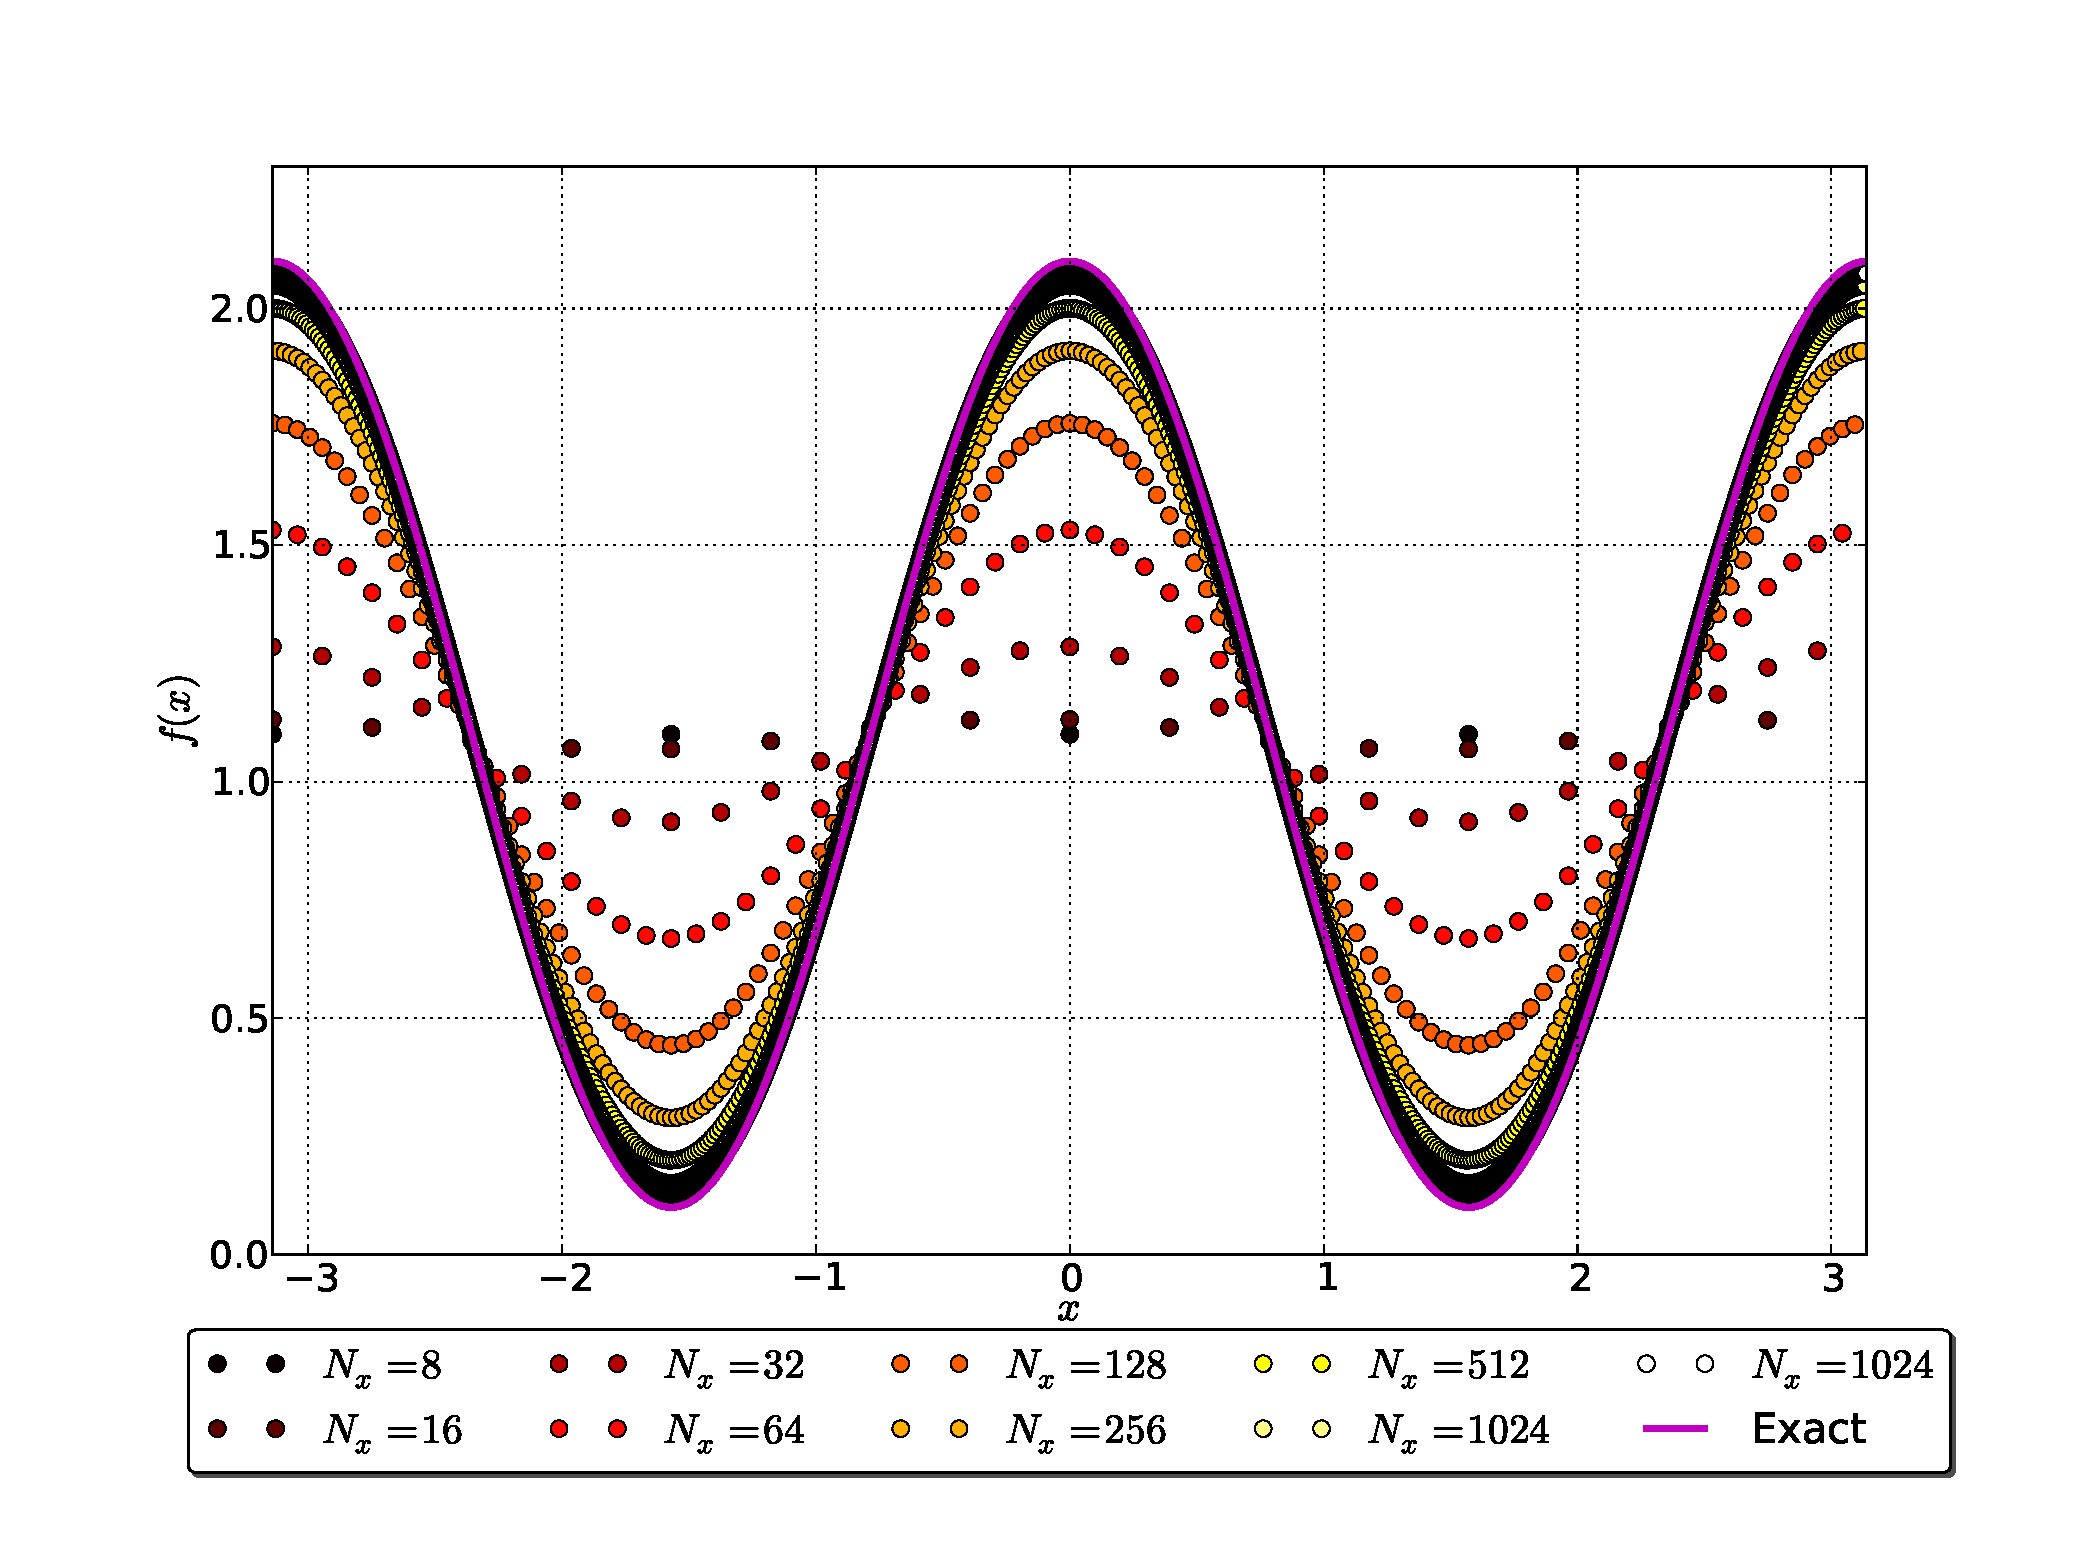
\includegraphics[width=\textwidth]{graphics/plot_-_ClassicCS_cosine2x_Nxall.eps}
 \caption{Several cases of the final solution obtained from the classic convected scheme algorithm are shown. For all simulations, the CFL number $\mathcal{C} = 0.32$. The figure records the number of spatial grid points $N_x$ ($N_t = N_x / 0.32$ for $\mathcal{C} = 0.32 = \text{constant}$). For coarse grids, even with their comparatively fewer remappings over a simulation time, the numerical diffusion spreads out the density significantly.}
 \label{fig:ClassicCS_cos2x_several_cases}
\end{figure}

To verify the higher order schemes have been implemented correctly, an order of accuracy exercise is pursued as before. However, for the corrected schemes, the above slowly varying initial distribution did not allow the order to be measured as the error too quickly approaches machine precision ($\epsilon \sim 10^{-16}$) even for coarse grids. Thus, a more irregular and challenging distribution is needed so that the effect of mesh refinement can be observed during the gradation. First, we examine numerical order of convergence of the \emph{FD5} method, which computes derivatives using finite differences. After which we verify spectral CS (\emph{FN} schemes) for various orders $N$.

Thus, we choose a non-periodic distribution that contains fine structure that must be adequately resolved relative to the order of accuracy of the scheme. The symmetric initial distribution (eq. \eqref{eq:GB3}) selected is a superposition of three Gaussian bells \cite{Guclu14}:

\begin{subequations}
\label{eq:GB3}
\begin{align}
f_0(x) & = \frac{1}{2}e^{-\left(\tfrac{x + 0.2}{0.03}\right)^2} + e^{-\left(\tfrac{x}{0.06}\right)^2} + \frac{1}{2}e^{-\left(\tfrac{x - 0.02}{0.03}\right)^2}  \\[0.8em]
x\in\mathcal{D} & = [-0.5, 0.5], \qquad t\in [0,1] 
\end{align}
\end{subequations}

\noindent the results are given in table \ref{tbl:FD5_order_GB3} whereas a representative solution is shown figure \ref{fig:FD5_GB3_Nx128} alongside the exact solution. additionally, Several cases are shown in figure \ref{fig:FD5_GB3_several_cases}.

\begin{table}
\centering
\makebox[0pt][c]{\parbox{1.1\textwidth}{%
\begin{minipage}{0.59\hsize}
\centering
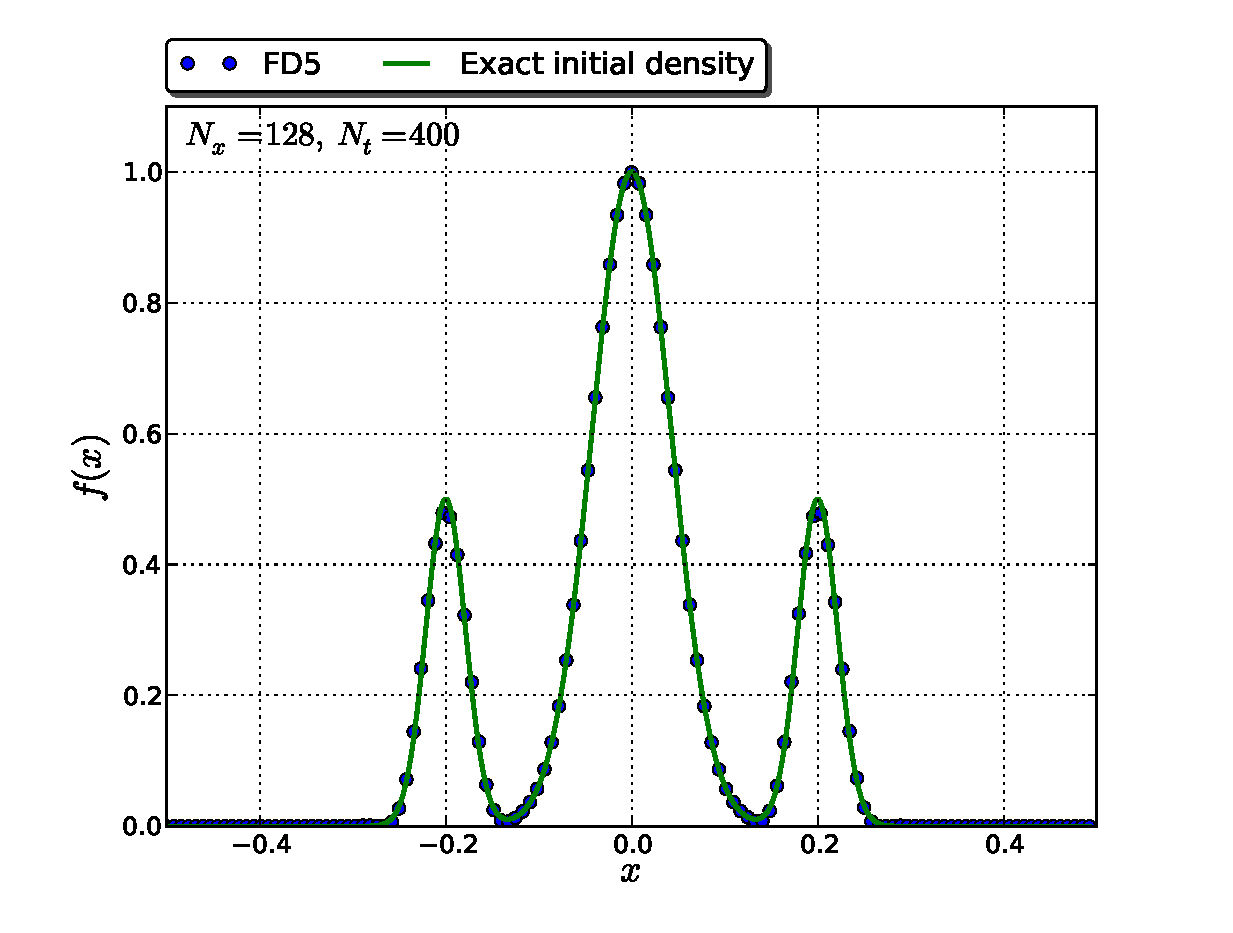
\includegraphics[width=1.1\hsize]{graphics/plot_-_GB3_FD5__Nx128Nt400_w_f0_itmax.eps}
\captionsetup{width=0.75\hsize}  \captionof{figure}{Numerical solution for FD5 after $N_t = 400$ time steps of eq. \eqref{eq:Advec_eq_1D_unit_vel} for $f_0$ given by \eqref{eq:GB3}.}
 \label{fig:FD5_GB3_Nx128}
\end{minipage}
\begin{minipage}{0.41\hsize}
\centering
\ra{1.3}\captionsetup{width=7cm}
\begin{tabular}{@{}llll@{}}\toprule
&\multicolumn{3}{c}{\phantom{$^2$ glob }FD5} \phantom{ClasicOrdera}\\
\cmidrule{2-4}& $\text{NRMS}(\text{GE}_{\Delta x})$ & Order \\ \midrule
$\phantom{a}N_x$\\
$\phantom{a}32$ & $7.2912\times 10^{-2}$ & $-$ \\
$\phantom{a}64$ & $2.5443\times 10^{-2}$ & 1.5189 \\
$\phantom{a}128$ & $4.4472\times 10^{-3}$ & 2.5163 \\
$\phantom{a}256$ & $2.1447\times 10^{-4}$ & 4.3741 \\
$\phantom{a}512$ & $7.0343\times 10^{-6}$ & 4.9302  \\
$\phantom{a}1024$ & $2.2142\times 10^{-7}$ & 4.9895 \\
$\phantom{a}2048$ & $6.9307\times 10^{-9}$ & \textcolor{red}{4.9976} \\
\bottomrule
\end{tabular}
\captionof{table}{Mesh refinement results for the FD5 scheme applied to the density \eqref{eq:GB3}. The normalized root mean square (NRMS) of the global error (GE) for each mesh with spacing $\Delta x = L/N_x$ is given by eq. \eqref{eq:GE}, and the observed numerical order of accuracy is computed per \eqref{eq:Order}. The CFL number $\mathcal{C} = 0.32$ for all simulations.The numerical order is converging towards $\mathcal{O}(\Delta x^5)$.}
\label{tbl:FD5_order_GB3}
\end{minipage}
}}
\end{table}

\begin{figure}[h!]
 \centering
   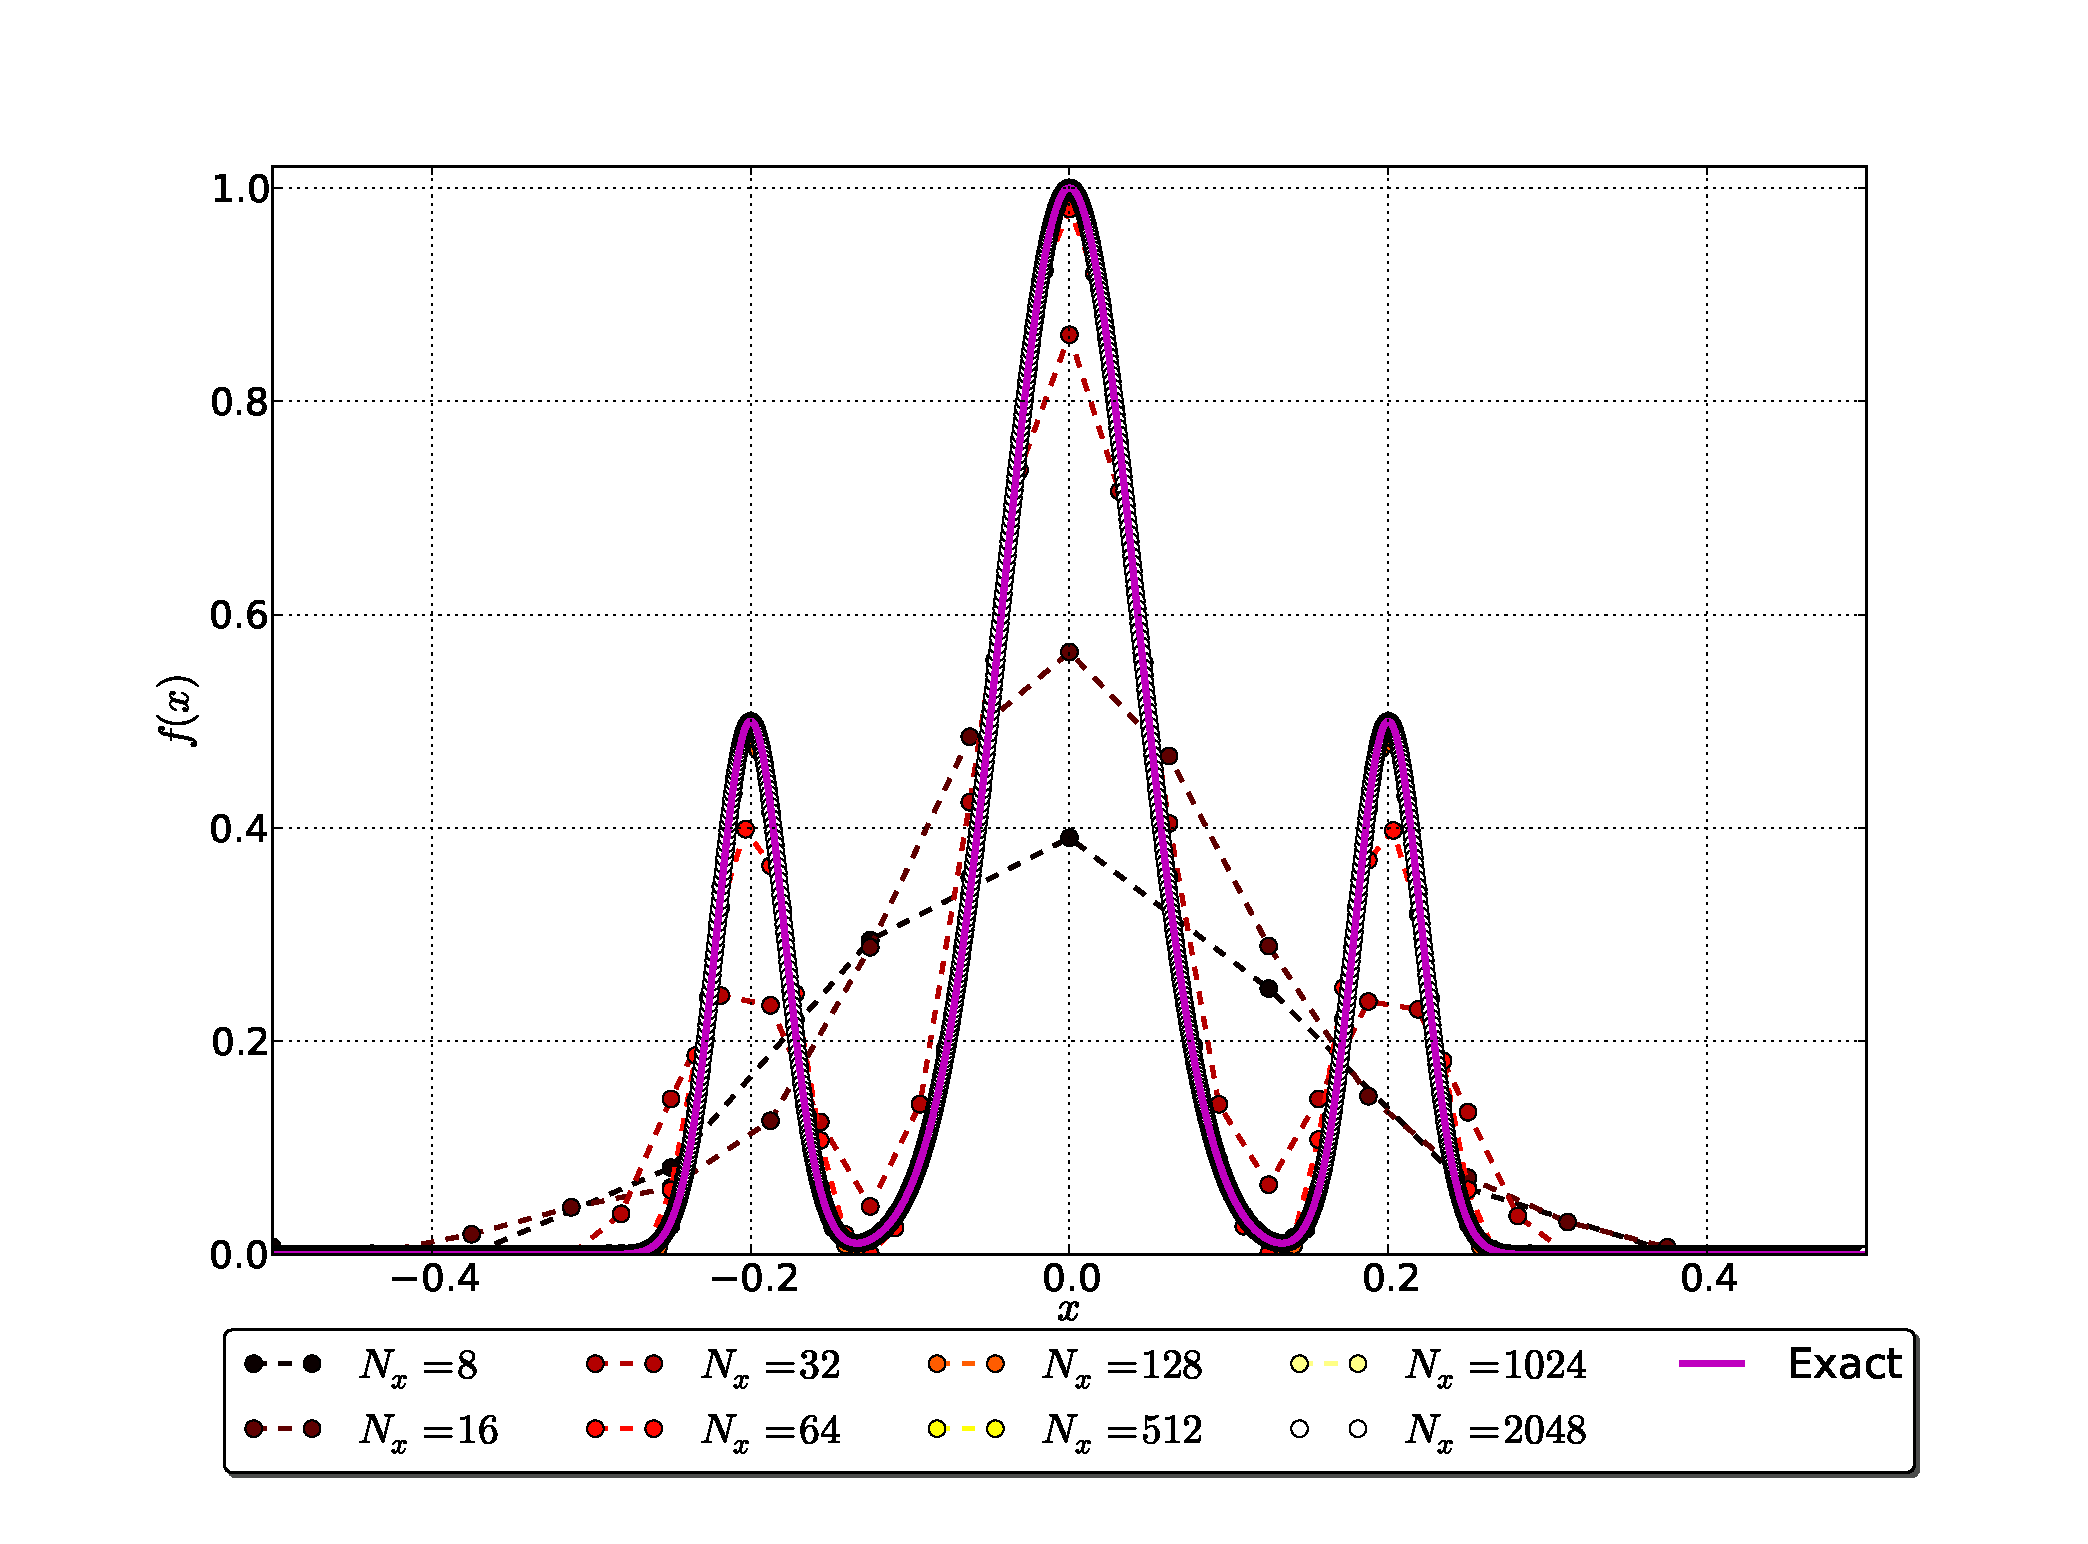
\includegraphics[width=\textwidth]{graphics/plot_-_GB3_FD5_Nxall_dashdot_w_Nx2048.eps}
 \caption{Several cases of the final solution obtained from the $N = 5$ order accurate \emph{FD5} scheme are shown. For all simulations, the CFL number $\mathcal{C} = 0.32$. The figure records the number of spatial grid points $N_x$ ($N_t = N_x / 0.32$ for $\mathcal{C} = 0.32 = \text{constant}$). With as coarse a mesh as $\textcolor{red}{N_x = 32}$ grid points the numerical solution is seen to retain the key features of the distribution (the three bells), and at $\textcolor{darkorange}{N_x = 128}$, the solution is seen to reasonably approximate the density.}
 \label{fig:FD5_GB3_several_cases}
\end{figure}

\noindent Even for meshes containing only $N_x = 32$, the corrected advected density maintains the shape of the three Gaussian bells, though the error is still visibly too significant. As few as $N_x = 128$ grid points gives a solution that has a NRMS global error of $4.4472\times 10^{-3}$ (table \ref{tbl:FD5_order_GB3}) and is seen to match the solution by inspection well (figure \ref{fig:FD5_GB3_Nx128}). The results clearly suggest a convergence towards $\mathcal{O}(\Delta x^5)$ as needed for the FD5 method.

To emphasize the previous motivation for using the cosine distribution \eqref{eq:cosine_2x} to verify the order for classic CS, the results for the classic convected scheme applied to the superposed Gaussian bell case \eqref{eq:GB3} above is summarized in table \ref{tbl:ClassicCS_order_GB3}, which shows the difficulty in proving numerical order of accuracy for the classic CS when considering more rapidly varying densities. Convergence was evidence as early as $N_x = 1024$ for the cosine distribution (cf. table \ref{tbl:ClassicCS_order_cos2x}), whereas for the following distribution, even at $N_x = 2048$ (order $\sim 0.7208$) the convergence is still not suggestive and the error is significant (figure \ref{fig:ClassicCS_GB3}).


\begin{table}
\centering
\makebox[0pt][c]{\parbox{1.1\textwidth}{%
\qquad\begin{minipage}{0.35\hsize}
\centering
\ra{1.3}\captionsetup{width=7cm}
\begin{tabular}{@{}llll@{}}\toprule
&\multicolumn{3}{c}{\phantom{$^2$ glob }Classic CS} \phantom{Ordera}\\
\cmidrule{2-4}& $\text{NRMS}(\text{GE}_{\Delta x})$ & Order \\ \midrule
$\phantom{a}N_x$\\
$\phantom{a}32$ & $2.0352\times 10^{-1}$ & $-$ \\
$\phantom{a}64$ & $1.9009\times 10^{-1}$ & 0.0985 \\
$\phantom{a}128$ & $1.6814\times 10^{-1}$ & 0.1770 \\
$\phantom{a}256$ & $1.3216\times 10^{-1}$ & 0.3474 \\
$\phantom{a}512$ & $9.2754\times 10^{-2}$ & 0.5108  \\
$\phantom{a}1024$ & $6.0219\times 10^{-2}$ & 0.6232 \\
$\phantom{a}2048$ & $3.6539\times 10^{-2}$ & 0.7208 \\
\bottomrule
\end{tabular}
\captionof{table}{Mesh refinement results for the classic convected scheme applied to the density \eqref{eq:GB3}. The normalized root mean square (NRMS) of the global error (GE) for each mesh with spacing $\Delta x = L/N_x$ is given by eq. \eqref{eq:GE}, and the observed numerical order of accuracy is computed per \eqref{eq:Order}. The CFL number $\mathcal{C} = 0.32$ for all simulations. The convergence of the numerical order of accuracy is not clear for this rapidly varying distribution. A much more resolved grid would be needed.}
\label{tbl:ClassicCS_order_GB3}
\end{minipage}
\hfill
\begin{minipage}{0.65\hsize}
\centering
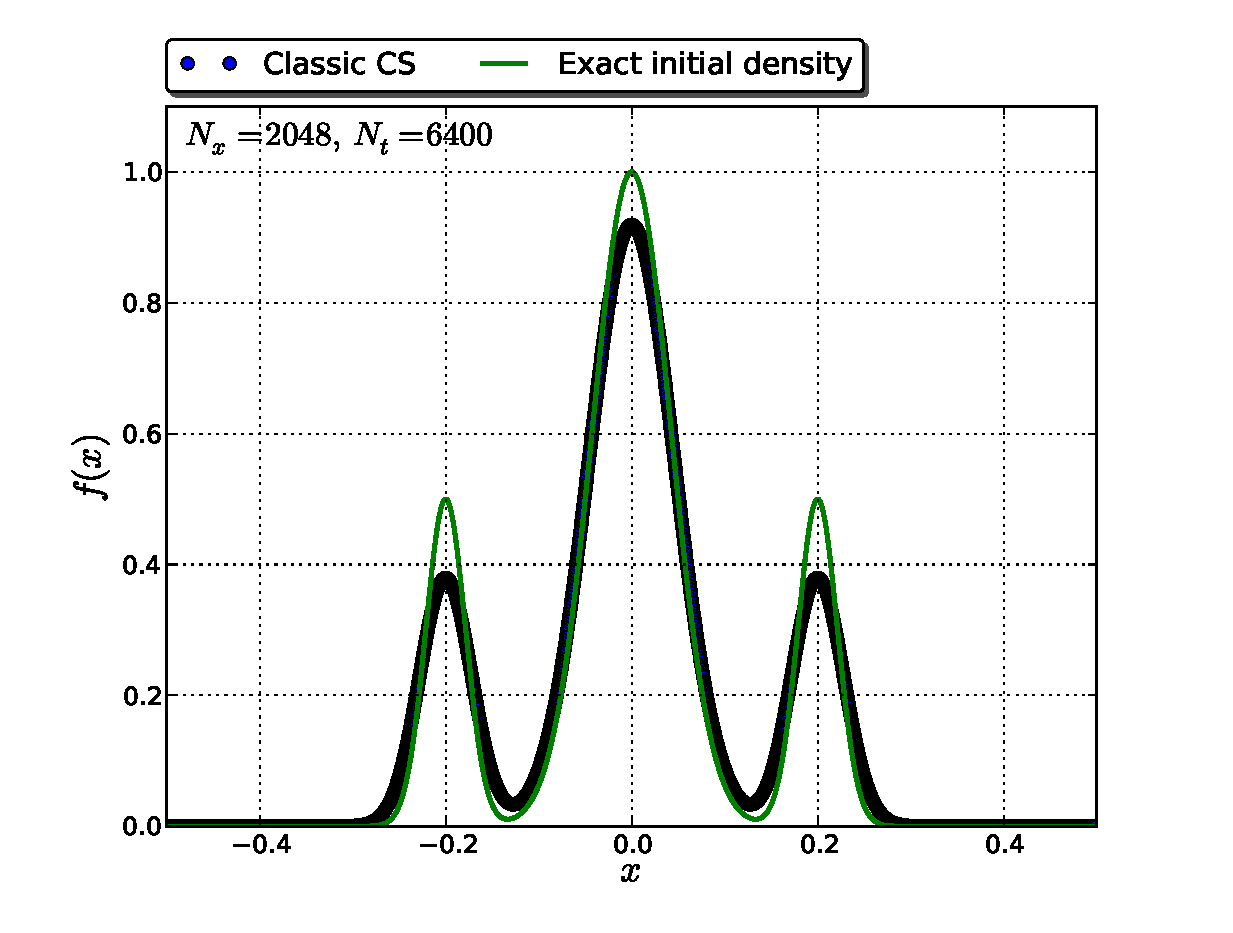
\includegraphics[width=\hsize]{graphics/plot_-_GB3_ClassicCS__Nx2048Nt6400_w_f0_itmax.eps}
\captionsetup{width=0.75\hsize}  \captionof{figure}{A classic CS solution after $N_t = 6400$ time steps of eq. \eqref{eq:Advec_eq_1D_unit_vel} for $f_0$ given by \eqref{eq:GB3}.}
 \label{fig:ClassicCS_GB3}
\end{minipage}
}}
\end{table}




With the classic CS and FD5 method verified, we move onto verifying $N$th order Fourier based (spectral) CS schemes (\emph{FN}). For orders $N \gtrsim 10$, the numerical order of accuracy is not directly measurable as the error approaches machine precision too soon in the mesh refinement exercise. In order to prove the implementation, we choose to instead verify each order $N$ as high as possible, and will take this as sufficient proof that higher orders follow suit. These results are summarized in table \ref{tbl:FN_order_calcs}.

\begin{landscape}
\begin{table}\centering
\ra{1.4}
\begin{tabular}{@{}lllcllcllclll@{}}\toprule[2 pt]
&\multicolumn{2}{c}{$F2$} & \phantom{abc} & \multicolumn{2}{c}{$F3$} &
\phantom{abc} & \multicolumn{2}{c}{$F4$} & \phantom{abc} & \multicolumn{2}{c}{$F5$} \\
\cmidrule{2-3} \cmidrule{5-6} \cmidrule{8-9} \cmidrule{11-12}  
& $\text{NRMS}(\text{GE}_{\Delta x})$ & Order && $\text{NRMS}(\text{GE}_{\Delta x})$ & Order && $\text{NRMS}(\text{GE}_{\Delta x})$ & Order  && $\text{NRMS}(\text{GE}_{\Delta x})$ & Order & \\ 
\midrule
\phantom{a}$N_x$ \\
\phantom{a}32	&	$9.3763\times 10^{-2}$	&	--	                 	&&	$5.3484\times 10^{-2}$	&	--               		&&	$2.1076\times 10^{-2}$	&	--              		&&	$1.8251\times 10^{-2}$	&	--	\\
\phantom{a}64	&	$4.7483\times 10^{-2}$	&	0.9816	                 	&&	$1.9892\times 10^{-2}$	&	1.4269           		&&	$4.9206\times 10^{-3}$	&	2.0987            		&&	$2.0776\times 10^{-3}$	&	3.1350	\\
\phantom{a}128	&	$2.06645\times 10^{-2}$	&	1.2003	                	&&	$4.4207\times 10^{-2}$	&	2.1698		                &&	$3.6497\times 10^{-4}$	&	3.7529            		&&	$8.0741\times 10^{-5}$	&	4.6855	\\
\phantom{a}256	&	$6.170\times 10^{-3}$	&	1.7436           		&&	$6.2759\times 10^{-4}$	&	2.8163          		&&	$2.2817\times 10^{-5}$	&	3.9996          		&&	$2.5658\times 10^{-6}$	&	4.9757	\\
\phantom{a}512	&	$1.5708\times 10^{-3}$	&	\textcolor{red}{1.9739}		&&	$8.0046\times 10^{-5}$	&	\textcolor{red}{2.9709}		&&	$1.4228\times 10^{-6}$	&	\textcolor{red}{4.0032}		&&	$8.0364\times 10^{-8}$	&	\textcolor{red}{4.9967}	\\
\midrule
&\multicolumn{2}{c}{$F6$} & \phantom{abc} & \multicolumn{2}{c}{$F7$} &
\phantom{abc} & \multicolumn{2}{c}{$F8$} & \phantom{abc} & \multicolumn{2}{c}{$F9$} \\
\cmidrule{2-3} \cmidrule{5-6} \cmidrule{8-9} \cmidrule{11-12}  
& $\text{NRMS}(\text{GE}_{\Delta x})$ & Order && $\text{NRMS}(\text{GE}_{\Delta x})$ & Order && $\text{NRMS}(\text{GE}_{\Delta x})$ & Order  && $\text{NRMS}(\text{GE}_{\Delta x})$ & Order & \\
\midrule
\phantom{a}$N_x$ \\
\phantom{a}32	&	$1.4003\times 10^{-2}$	&	--              		&&	$1.3743\times 10^{-2}$	&	--                 		&&	$1.3757\times 10^{-2}$	&	--	                	&&	$1.3711\times 10^{-2}$	&	--	\\
\phantom{a}64	&	$4.7357\times 10^{-4}$	&	4.8860            		&&	$2.2053\times 10^{-4}$	&	5.9615               		&&	$5.6229\times 10^{-5}$	&	7.934635	                &&	$3.0591\times 10^{-5}$	&	8.808078	\\
\phantom{a}128	&	$7.7235\times 10^{-6}$	&	5.9381                		&&	$1.9207\times 10^{-6}$	&	6.8432          		&&	$2.1371\times 10^{-7}$	&	\textcolor{red}{8.039495}	&&	$5.8963\times 10^{-8}$	&	\textcolor{red}{9.019098}	\\
\phantom{a}256	&	$1.1945\times 10^{-7}$	&	\textcolor{red}{6.0147}		&&	$1.5166\times 10^{-8}$	&	\textcolor{red}{6.9847}		&&	$8.2396\times 10^{-10}$	&	8.018886                 	&&	$1.1657\times 10^{-10}$	&	8.982388	\\
\phantom{a}512	&	$1.8608\times 10^{-9}$	&	6.0042           		&&	--	                &	--              		&&	--	                &	--                     		&&	--	                &	--	\\
\midrule
&\multicolumn{2}{c}{$F10$} & \phantom{abc} & \multicolumn{2}{c}{$F11$} &
\phantom{abc} & \multicolumn{2}{c}{$F12$} & \phantom{abc} & \multicolumn{2}{c}{$F13$} \\
\cmidrule{2-3} \cmidrule{5-6} \cmidrule{8-9} \cmidrule{11-12}  
& $\text{NRMS}(\text{GE}_{\Delta x})$ & Order && $\text{NRMS}(\text{GE}_{\Delta x})$ & Order && $\text{NRMS}(\text{GE}_{\Delta x})$ & Order  && $\text{NRMS}(\text{GE}_{\Delta x})$ & Order & \\
\midrule
\phantom{a}$N_x$ \\
32	&	$1.3742\times 10^{-2}$	&	--          		&&	$1.3733\times 10^{-2}$	&	--		        &&	$1.3736\times 10^{-2}$	&	--		&&	$1.3734\times 10^{-2}$	&	--	\\
64	&	$1.4822\times 10^{-5}$	&	9.8566       		&&	$1.3397\times 10^{-5}$	&	10.0014		        &&	$1.2761\times 10^{-5}$	&	10.0721		&&	$1.2718\times 10^{-5}$	&	10.0766	\\
128	&	$7.3664\times 10^{-9}$	&	10.9745 		&&	$2.2175\times 10^{-9}$	&	12.5607		        &&	$3.0450\times 10^{-10}$	&	15.3548		&&	$9.8644\times 10^{-11}$	&	16.9763	\\
256	&	$7.0799\times 10^{-12}$	&	\textcolor{red}{10.0230}&&	$1.1011\times 10^{-12}$	&	10.9758&&	$9.7125\times 10^{-14}$	&	$(m.p.)$		&&	$6.7652\times 10^{-14}$	&	$(m.p.)$	\\
512	&	$1.0166\times 10^{-13}$	&	$(m.p.)$		&&	$1.0180\times 10^{-13}$	&	$(m.p.)$		&&	$1.0187\times 10^{-13}$	&	$(m.p.)$		&&	$1.0182\times 10^{-13}$	&	$(m.p.)$	\\
\bottomrule[2 pt]
\end{tabular}
\caption{Order calculations (eq. \eqref{eq:GE}) for various orders of spectral CS. For $N \gtrsim 10$, the order of convergence cannot be observed as machine precision $(m.p.)$ is achieved too soon. The calculations highlighted in \textcolor{red}{red} indicate when convergence is sufficiently suggestive.}
\label{tbl:FN_order_calcs}
\end{table}
\end{landscape}

\noindent Thus, since the numerical order of accuracy is convincingly observed for orders $N = 2$ to $N = 10$ in the $FN$ schemes, it can only be expected that the higher orders must follow suit. We regard this as sufficient proof of implementation for the $FN$ methods. For orders $N \geq 18$, machine precision is obtained for grids with as few points as $N_x = 128$. While the Fourier-based CS scheme is very efficient, the computational cost increases significantly with each order of accuracy. The simulation times for several orders of accuracy $N$ for $FN$ schemes are compared in table \ref{tbl:FN_simtimes} for serial processing of a Python implemented CS on a 3.4 GHz CPU with 8 GB of RAM.  Regarding the spectral CS \hyperlink{alg:3}{algorithm 3}, we note that computing corrections required for the next higher order requires computing $N_x$ additional derivatives per time step, and $N_xN_t$ derivatives over a full simulation. Each derivative amounts to one complex multiplication operation in Fourier space to compute the derivative coefficients $\hat{d}_q^n$, which still requires recursively calculating the next $\beta_{N-1}(\alpha )$ coefficient (eq. \eqref{eq:beta_q}), and so on. Thus, it is clear that the processor time quickly increases as the order $N$ becomes large. With computational expense and accuracy in mind, we consult table \ref{tbl:FN_simtimes} and the errors found from test cases to come to the decision of selecting the 15th order accurate method ($F15$) to use henceforth. The F15 method achieves machine precision for the Gaussian bell test case at $N_x = 256$ (table \ref{tbl:F15_order_GB3}), and requires only minutes to complete a full simulation under this model case. A plot of the numerical solution for this scheme is shown in figure \ref{fig:F15_Nx128_GB3}.

\begin{table}
\centering
\makebox[0pt][c]{\parbox{1.1\textwidth}{%
\qquad\begin{minipage}{0.35\hsize}
\centering
\ra{1.3}\captionsetup{width=7cm}
\begin{tabular}{@{}llll@{}}\toprule
&\multicolumn{3}{c}{\phantom{$^2$ glob }$F15$} \phantom{ClasicOrdera}\\
\cmidrule{2-4}& $\text{NRMS}(\text{GE}_{\Delta x})$ & Order \\ \midrule
$\phantom{a}N_x$\\
$\phantom{a}32$ & $1.3733\times 10^{-2}$ & $-$ \\
$\phantom{a}64$ & $1.2690\times 10^{-5}$ & 10.079 \\
$\phantom{a}128$ & $5.0649\times 10^{-12}$ & 21.257 \\
$\phantom{a}256$ & $6.6473\times 10^{-14}$ & $(m.p.)$ \\
\bottomrule
\end{tabular}
\captionof{table}{Mesh refinement results for the spectral CS $F15$ scheme applied to the density \eqref{eq:GB3}. The normalized root mean square (NRMS) of the global error (GE) for each mesh with spacing $\Delta x = L/N_x$ is given by eq. \eqref{eq:GE}, and the observed numerical order of accuracy is computed per \eqref{eq:Order}. The CFL number $\mathcal{C} = 0.32$ for all simulations. The term $(m.p.)$ indicates the solution has reached machine precision, and the order of convergence is not directly observable.}
\label{tbl:F15_order_GB3}
\end{minipage}
\hfill
\begin{minipage}{0.65\hsize}
\centering
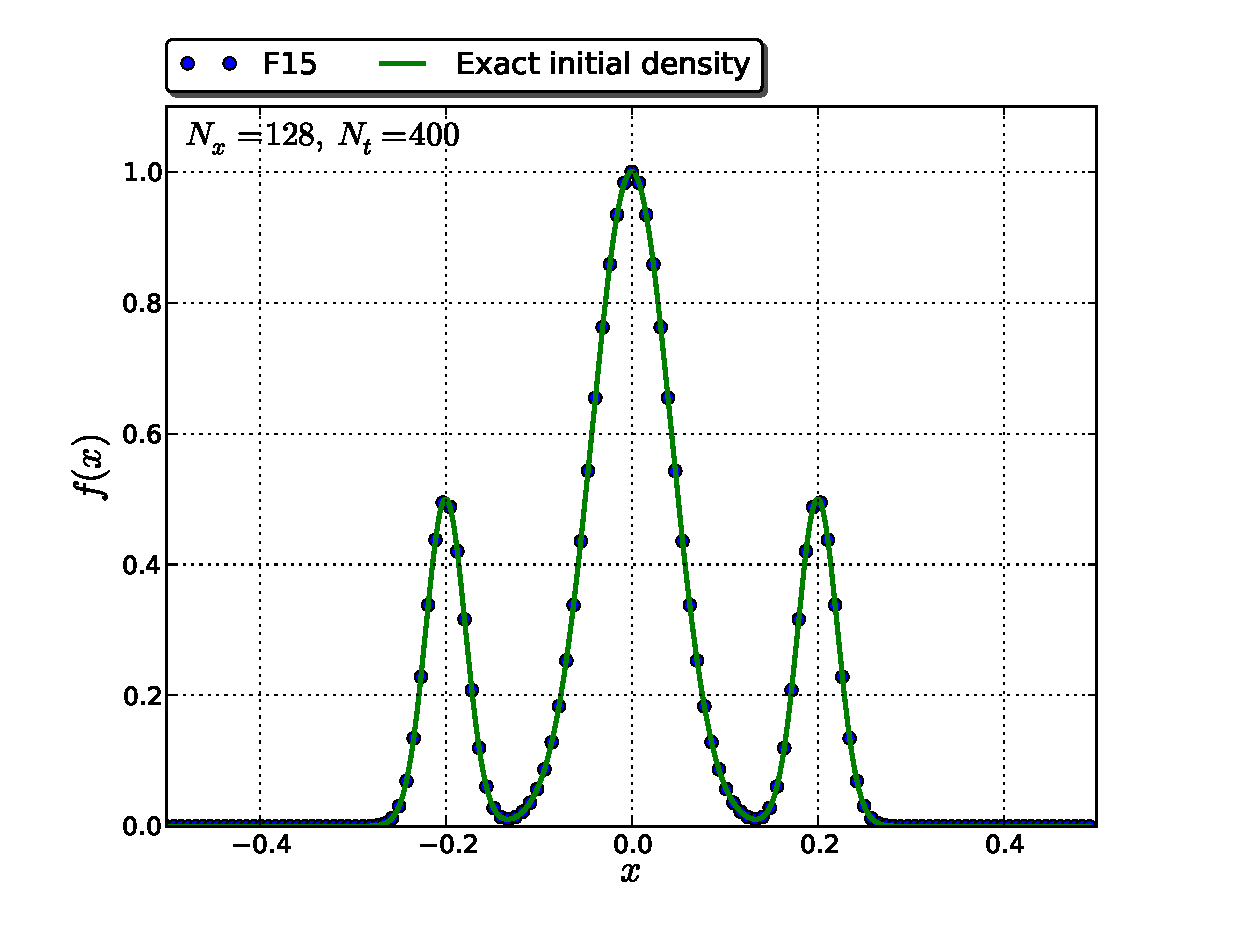
\includegraphics[width=\hsize]{graphics/plot_-_GB3_F15__Nx128Nt400_w_f0_itmax.eps}
\captionsetup{width=0.75\hsize}  \captionof{figure}{An F15 solution after $N_t = 400$ time steps of eq. \eqref{eq:Advec_eq_1D_unit_vel} for $f_0$ given by \eqref{eq:GB3}.}
 \label{fig:F15_Nx128_GB3}
\end{minipage}
}}
\end{table}

\begin{table}\centering
\ra{1.4}
\begin{tabular}{@{}llcllclcl@{}}\toprule[2 pt]
&\multicolumn{1}{c}{$N_x = 64$} & \phantom{abc} & \multicolumn{1}{c}{$N_x = 128$} & \phantom{abc} & \multicolumn{1}{c}{$N_x = 64$} & \phantom{abc} & \multicolumn{1}{c}{$N_x = 128$} &\\
\cmidrule{2-2}  \cmidrule{4-4} \cmidrule{6-6} \cmidrule{8-8}
& Processor time [sec] && Processor time [sec] && Processor time [sec] && Processor time [sec] \\
\midrule
\phantom{a}$FN$ & && & \phantom{a}$FN$ \\
\phantom{a}$F2$	&	$5.4000\times 10^{-1}$	&&	$2.1900\phantom{\times 10^{-2}}$	&	\phantom{a}$F12$		 & 	$3.4920\times 10^{1}$	 && 	$7.1450\times 10^{1}$		\\
\phantom{a}$F3$	&	$7.2000\times 10^{-1}$	&&	$2.7900\phantom{\times 10^{-2}}$	&	\phantom{a}$F13$		 & 	$6.7950\times 10^{1}$	 && 	$1.3566\times 10^{2}$		\\
\phantom{a}$F4$	&	$8.8000\times 10^{-1}$	&&	$3.4000\phantom{\times 10^{-3}}$	&	\phantom{a}$F14$		 & 	$1.3281\times 10^{2}$	 && 	$2.6560\times 10^{2}$		\\
\phantom{a}$F5$	&	$1.0500\phantom{\times 10^{-2}}$	&&	$3.7700\phantom{\times 10^{-3}}$	&	\phantom{a}$F15$		 & 	$2.6576\times 10^{2}$	 && 	$5.3762\times 10^{2}$		\\
\phantom{a}$F6$	&	$1.4700\phantom{\times 10^{-2}}$	&&	$4.8100\phantom{\times 10^{-4}}$	&	\phantom{a}$F16$		 & 	$5.3070\times 10^{2}$	 && 	$1.0863\times 10^{3}$		\\
\phantom{a}$F7$	&	$2.0600\phantom{\times 10^{-2}}$	&&	$6.0900\phantom{\times 10^{-4}}$	&	\phantom{a}$F17$		 & 	$1.0794\times 10^{3}$	 && 	$2.1287\times 10^{3}$		\\
\phantom{a}$F8$	&	$3.1700\phantom{\times 10^{-2}}$	&&	$8.5700\phantom{\times 10^{-5}}$	&	\phantom{a}$F18$		 & 	$2.1190\times 10^{3}$	 && 	$4.1185\times 10^{3}$		\\
\phantom{a}$F9$	&	$5.3800\phantom{\times 10^{-2}}$	&&	$1.3250\times 10^{1}$	&	\phantom{a}$F19$		 & 	$4.2417\times 10^{3}$	 && 	$4.1786\times 10^{3}$		\\
\phantom{a}$F10$	&	$9.8700\phantom{\times 10^{-2}}$	&&	$2.2260\times 10^{1}$	&	\phantom{a}$F20$		 & 	$9.3585\times 10^{3}$	 && 	$1.8601\times 10^{4}$		\\
\phantom{a}$F11$	&	$1.7850\times 10^{1}$	&&	$3.8110\times 10^{1}$	&	\phantom{a}$F21$		 & 	$1.1111\times 10^{1}$	 && 	$1.1111\times 10^{1}$		\\
\bottomrule[2 pt]
\end{tabular}
\caption{Processor times required to compute a numerical solution to advection equation \eqref{eq:Advec_eq_1D_unit_vel} with the initial distribution of the superposed Gaussian bell density \eqref{eq:GB3} for various order $N$ for spectral CS ($FN$). The processor time picks up significantly for order $N \gtrsim 15$. For a 20th order accurate method on a grid of $N_x = 128$ points (at machine precision, the global $L^2$ error $ = 6.7205\times 10^{-15}$), simulations for this Python-implemented CS algorithm requires around 5.01 hours on serial processing with a 3.4 GHz CPU and 8 GB RAM. A 15th order method at the same resolution requires only 9 minutes ($L^2$ error $ = 5.0649\times 10^{-12}$) The errors for orders up to $N = 13$ are provided in \ref{tbl:FN_order_calcs}.}
\label{tbl:FN_simtimes}
\end{table}


\subsection{1D advection: variable velocity}

\indent \indent The corrections are modeled to the one-speed advection equation. However, the implementation on a computer is such that the equation is solved for one moving cell (MC) at a time. Thus, the correction and methods develop apply to non-constant speeds, since each problem itself is a one-speed problem. To this end, we extend the code to permit the scenario variable velocity fields. In particular, we examine a spatially-dependent velocity field in one dimension. 

\begin{subequations}
\label{eq:Advec_eq_1D_unit_vel}
\begin{align}
\frac{\partial f}{\partial t} + v(x)\frac{\partial f}{\partial x} =  0, &\qquad x\in\mathcal{D}, t\in [0,T] \label{eq:1D_advec_equation_var_vel}\\[1em]
f(0,x) = f_0(x) \\[1em]
f(t,x + L) = f(t,x)
\end{align}
\end{subequations}


\noindent Such circumstances are familiar in fluid mechanics where the local speed of a fluid parcel can be tracked by an independent variable that parameterizes the pathlines of the fluid flow (e.g. a physical stream where the parcel speed increases along pathlines that suffer elevation drops). The numerical solution over time is computed for an initial condition given by an (unnormalized) Gaussian with a narrow peak $f_0 \sim \mathcal{N}(0,0.04)$, and a sinusoidal velocity field $v_S(x)$, i.e.

\begin{equation}
f_0(x) = e^{-x^2 / (2(0.04)^2)}, \qquad \text{and } \qquad v_S(x) = \sin 2\pi x, \qquad x\in [-0.5, 0.5]
\end{equation}

\noindent Thus, the domain covers one full period of the velocity function and the Gaussian distribution has compact support close to the origin. 

 \begin{figure}[h!]
  \centering
    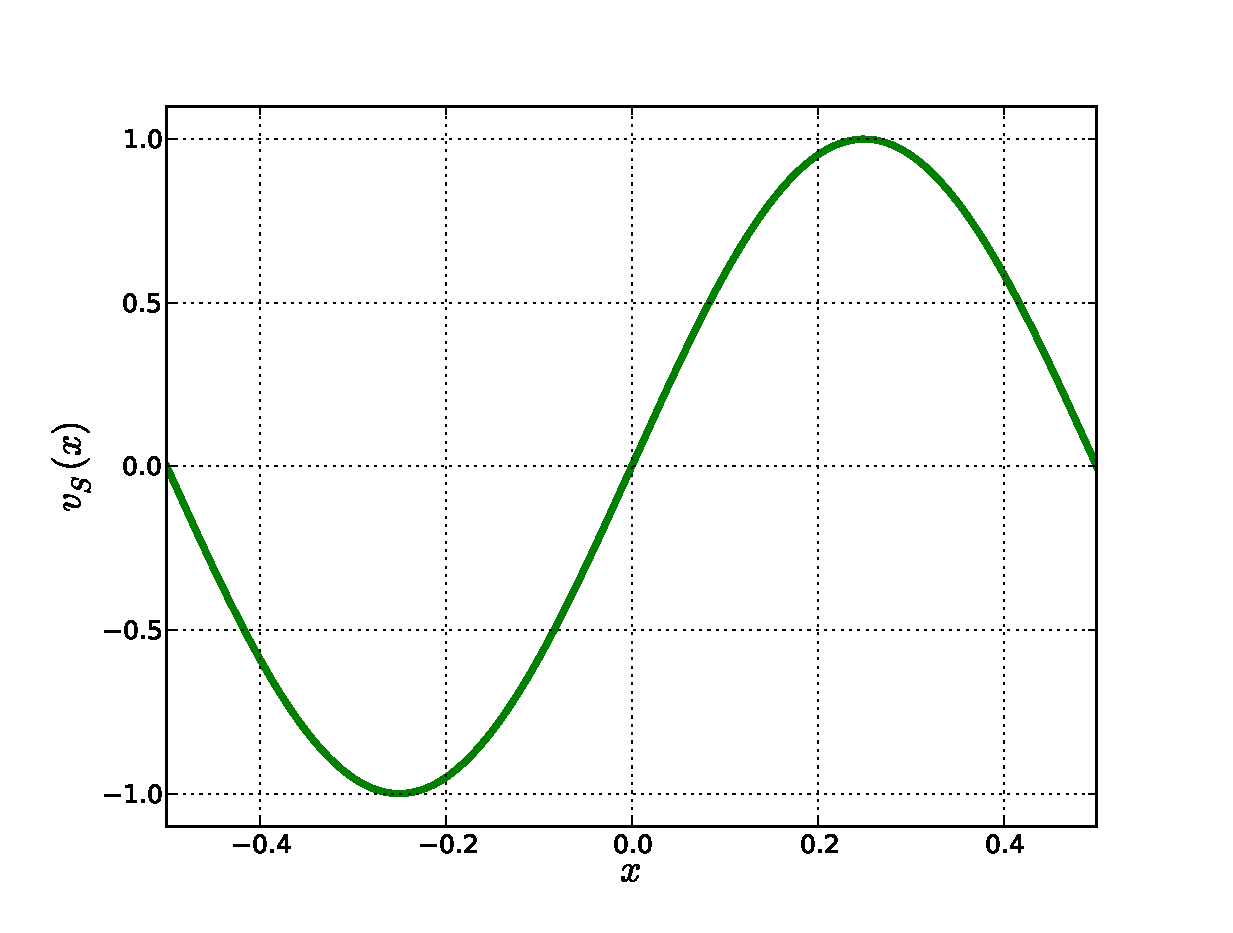
\includegraphics[width=0.45\textwidth]{graphics/v_S}
  \caption{the velocity field varies as a function of position.}
  \label{fig:v_S}
\end{figure}

\noindent The solution is stepped through in the figures below as computed with the $F15$ scheme on a mesh with $N_x = 256$ cells over  $N_t = 400$ time steps until a final time $T = 1.0$ (CFL number $\mathcal{C} = 0.32$). The initial distribution (shown in \textcolor{darkgreen}{green}) is plotted alongside the instantaneous solution (\textcolor{blue}{blue}) for comparison. Note, from the figures it is seen that the density at $x = 0$ stays put throughout the simulation as $v_S(x=0) = 0$.

\begin{figure}[h!] 
\label{fig:var_vel}
\captionsetup{width=0.48\linewidth}
\begin{minipage}[b]{0.5\linewidth}
\centering
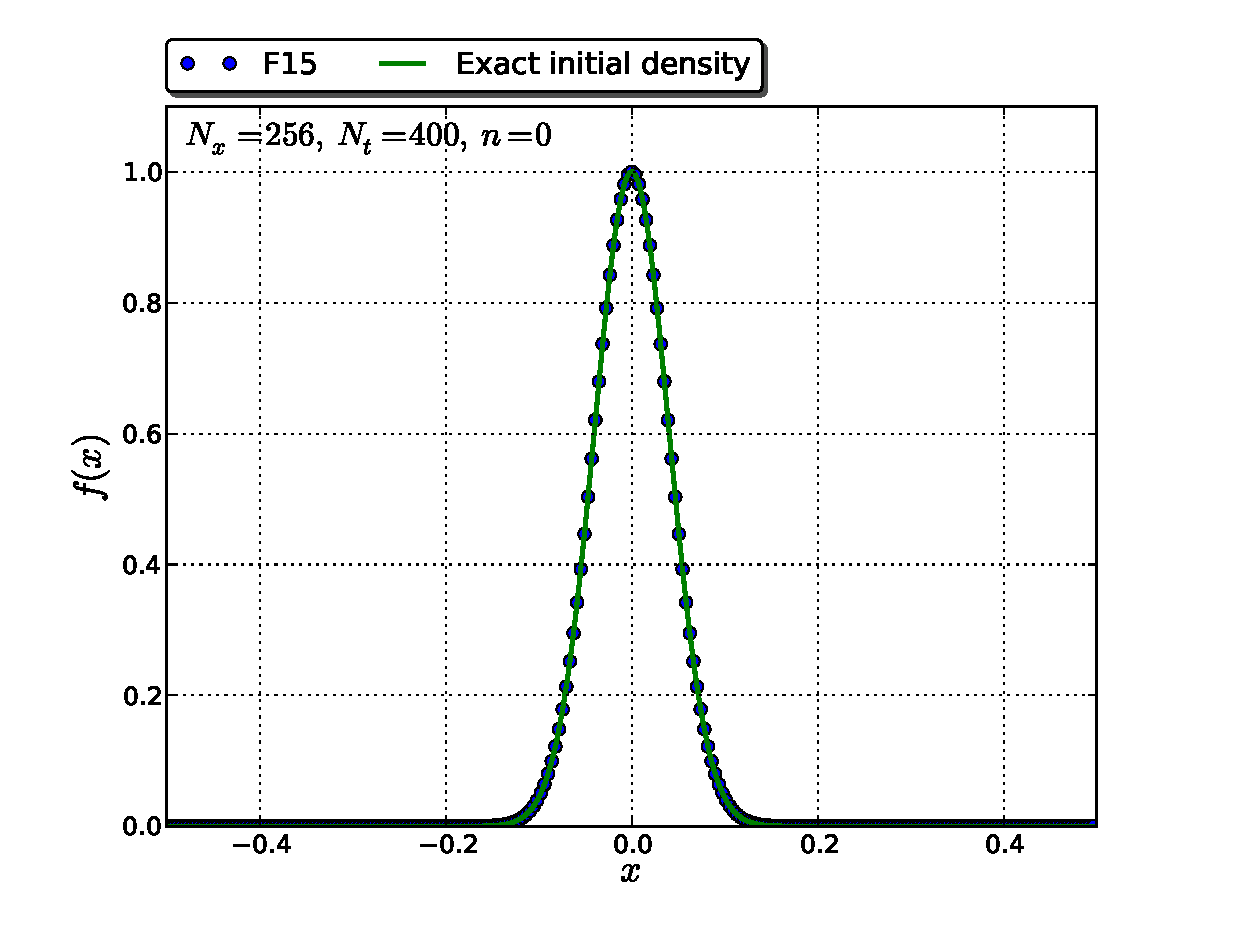
\includegraphics[width=\linewidth]{graphics/f_N_v_S_F15_Nx256Nt400_w_f0_it00000}
\caption{Variable density test case: $t^0 = 0$}
\vspace{4ex}
\end{minipage}%%
\begin{minipage}[b]{0.5\linewidth}
\centering
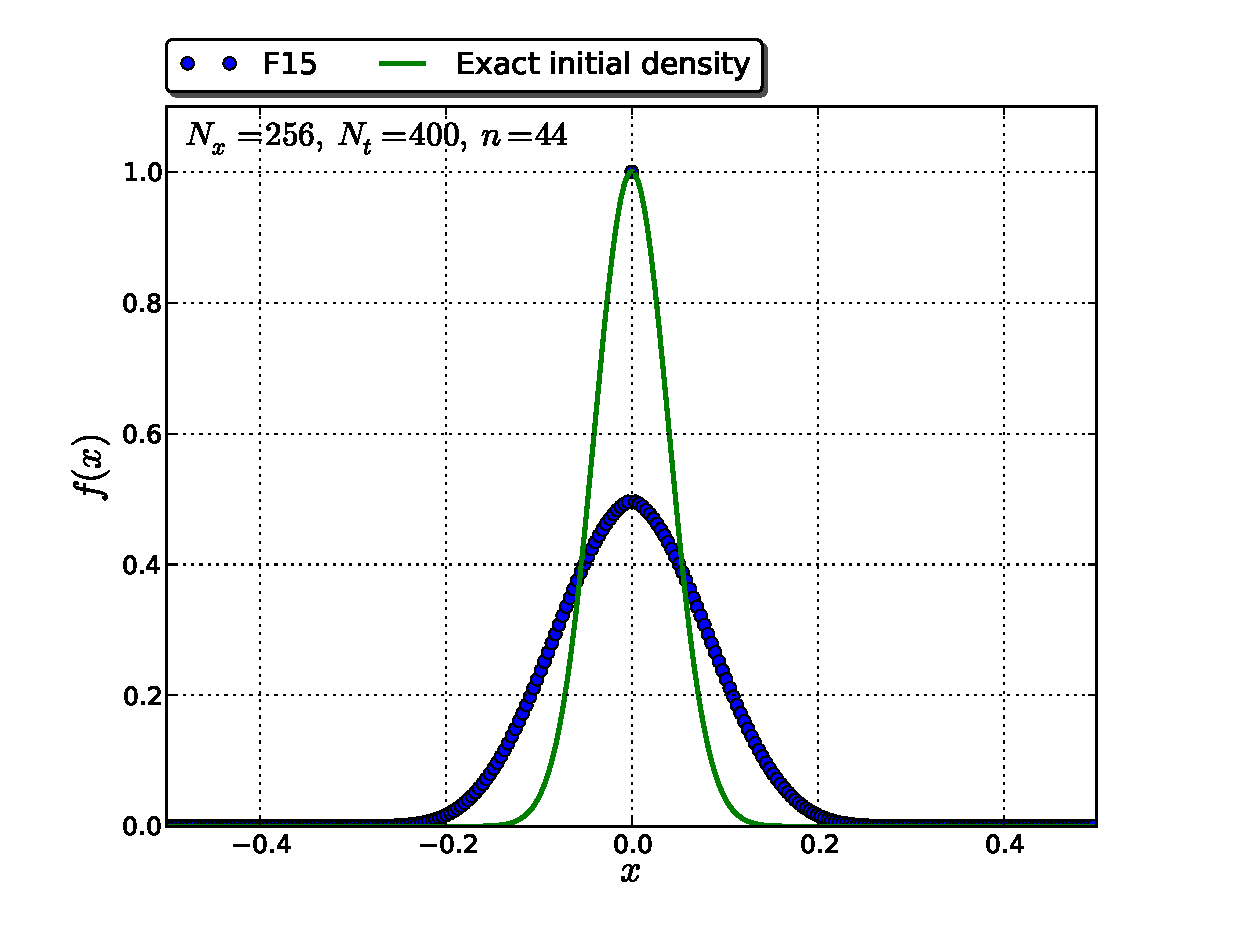
\includegraphics[width=\linewidth]{graphics/f_N_v_S_F15_Nx256Nt400_w_f0_it00044}
\caption{Variable density test case: time $t^{44} = 0.11$}
\vspace{4ex}
\end{minipage} 
\begin{minipage}[b]{0.5\linewidth}
\centering
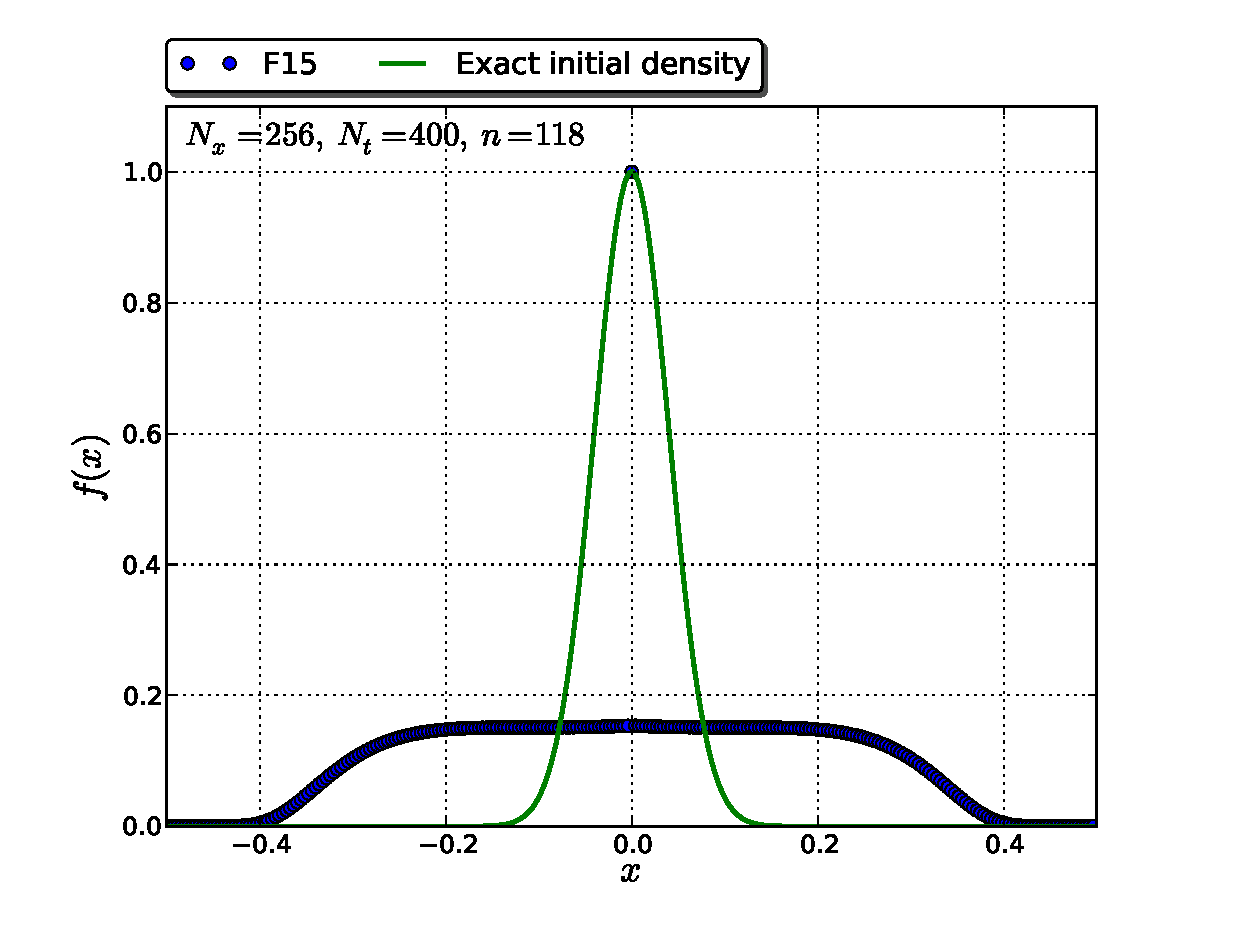
\includegraphics[width=\linewidth]{graphics/f_N_v_S_F15_Nx256Nt400_w_f0_it00118}
\caption{Variable density test case: time $t^{118} = 0.295$}
\vspace{4ex}
\end{minipage}%% 
\begin{minipage}[b]{0.5\linewidth}
\centering
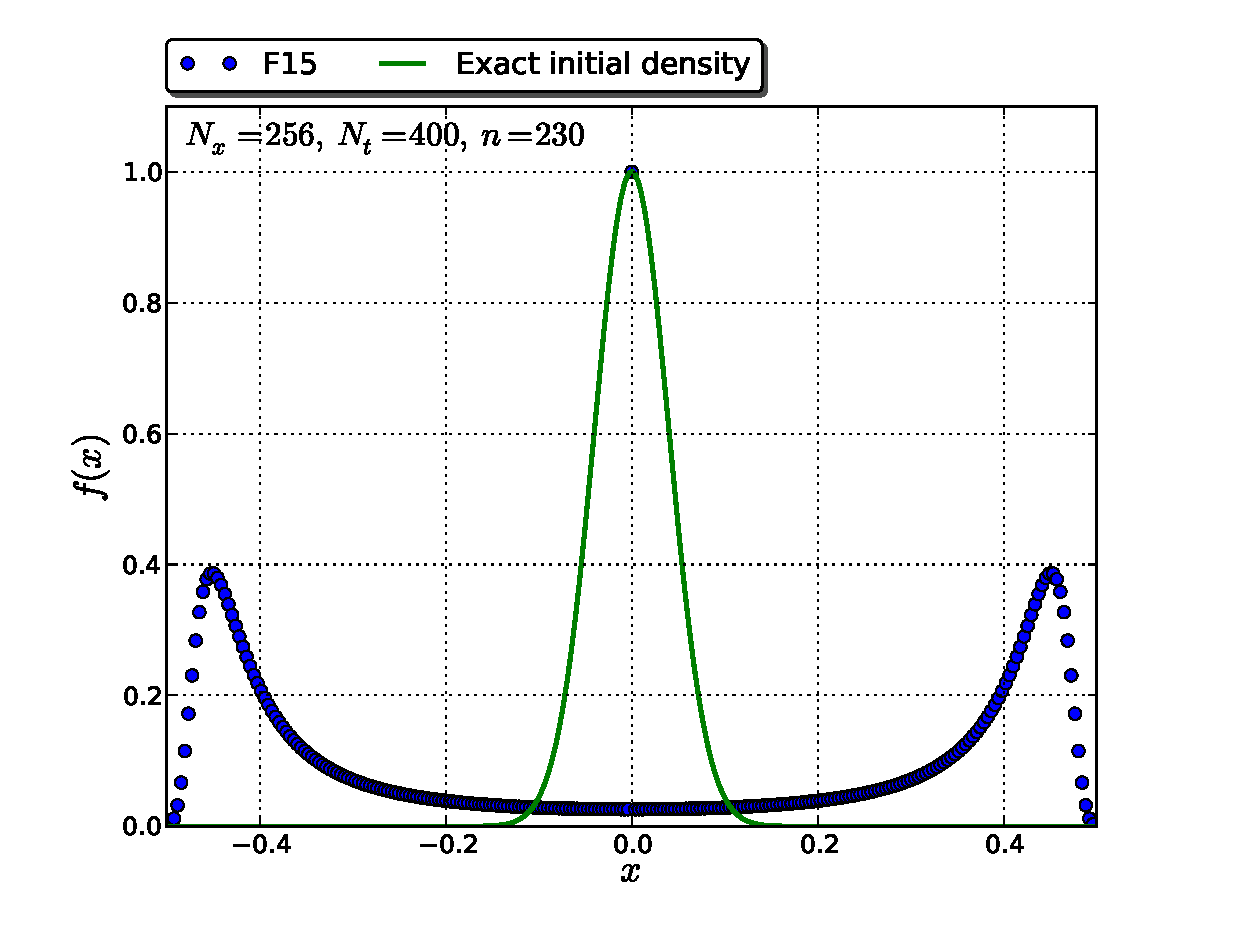
\includegraphics[width=\linewidth]{graphics/f_N_v_S_F15_Nx256Nt400_w_f0_it00230}
\caption{Variable density test case: time $t^{230} = 0.575$}
\vspace{4ex}
\end{minipage} 
\end{figure}

Discussing the snapshots shown in the series of figures, we see that soon after the simulation start time ($t^0 = 0$), the oppositely directed velocities near the origin convect densities left and right to spread out the profile (seen in at time $t^{44}$). As more density is advected left (resp. right) the density encounters regions where the velocities become increasingly negative (resp. positive) which accelerates the spreading of the distribution as evident at time $t^{118}$. The velocity magnitudes increase in both directions in $x$ until the turning points at $x = \pm 0.25$ (see figure \ref{fig:v_S}) whereafter the magnitudes decrease in both directions towards the edges of the domain. Density travelling beyond these points encounter slower speeds so that density ahead of the velocity extrema ($x = \pm 0.25$) is advected slower than that behind it (within $|x| < 0.25$). The pushed density from behind accumulates in slower regions so that the effect at time $t^{230}$ results. The trend continues until the final time step until density is pushed against the walls of the domain, leaving mostly zero density inside by the end of simulation time $t^{400} = 1$.


\subsection{2D rotating advection system: time splitting schemes analysis}

\indent \indent Splitting is necessary to move onto the next order of complication in the immediate goal to apprehend the Vlasov-Poisson system (cf. section \ref{section:The_semi_Lagrangian_approach_to_the_Vlasov_Poisson_system}). As a next step, we consider a two-dimensional advection equation with velocity field $\vec{v}(x,y) = \langle v_x,v_y \rangle$:

\begin{subequations}
\label{eq:Advec_eq_1D_unit_vel}
\begin{align}
\frac{\partial f}{\partial t} + v_x(x,y)\frac{\partial f}{\partial x} + v_y(x,y)\frac{\partial f}{\partial y} =  0, &\qquad (x,y)\in\mathcal{D}, t\in [0,T] \label{eq:2D_advec_equation_general}\\[1em]
f(0,x,y) = f_0(x,y) \\[1em]
f(t,x + L,y) = f(t,x,y), & \quad f(t,x,y+L) = f(t,x,y)
\end{align}
\end{subequations}

The model case is the system investigated by \cite{Guclu14} which convects a 22nd order ``cosine cross'' density packet in a rotating velocity field about the origin, which is characterized by a frequency $\omega = 2\pi / P$ where $P$ is the period for a full revolution. For clockwise rotation we have

\begin{equation}v_x(y) = \omega y, \qquad \text{and } \qquad v_y(x) = -\omega x\end{equation}

\noindent We choose a period $P = 1$ so that one full revolution is executed in unit time $T = 1$ (i.e. $\omega = 2\pi$). We also select a domain $\mathcal{D}= [-1,1]\times [-1,1]$, along with the aforementioned cosine cross initial density. This particular function was chosen by G\"{u}\c{c}lu with the intention to use the $F21$ corrected scheme (N.B. this scheme is labeled as $F22$ in \cite{Guclu14} due a difference in what they define as an $N$th order method). Choosing a 22nd order cosine bell ($C^{21}(\mathbb{R}^2)$) ensures we have the required $N - 1$ derivatives needed to correct the CS up to N = 21, or $\mathcal{O}(\Delta x^{21}, \Delta y^{21})$ in space (cf. page \pageref{pg:deriv_reqs} and eq. \eqref{eq:Uf}). Using a corrected scheme on a sufficiently resolved grid so that the accuracy in space is at machine precision permits the splitting error in time to be observed (section \ref{subsec:Operator_splitting_theory}). To this end, we elect to use an $F12$ method with $N_x = N_y = 256$ grid points, as previous convergence analysis has shown that we are well below machine precision and save some computational cost by not using a higher order method. 

Thus, the rotating system to be analyzed is a solution to the following:

\begin{equation}
\frac{\partial f}{\partial t} + 2\pi y\frac{\partial f}{\partial x} - 2\pi x\frac{\partial f}{\partial y} =  0, \qquad (x,y)\in [-1,1]\times [-1,1], t\in [0,T] \label{eq:2Drot_advec_eq}
\end{equation}

\noindent The initial density eq. \eqref{eq:cosine_cross} is a superposition of two mutually transverse cosine bells whose cross-section has a major radius $2a = 0.5$, both of which are centered at a position $(x_c,y_c) = (0,0.5)$ at time $t = 0$. A contour plot is given alongside the function definition in figure \ref{fig:f0_2drot}.

\begin{table}
\centering
\makebox[0pt][c]{\parbox{1.1\textwidth}{%
\qquad\begin{minipage}{0.41\hsize}
\ra{1.3}\captionsetup{width=7cm}
\begin{equation}
f_0(x,y) = 0.5 B(r_1(x,y)) + 0.5 B(r_2(x,y)) \label{eq:cosine_cross}
\end{equation}
\begin{subequations}
\begin{align}
 B(r,a) &=
  \begin{cases}
  \cos^{22}\left(\tfrac{\pi r}{2a}\right) & \text{for } r \leq a \\[0.5em]
   0       & \text{else }
  \end{cases}\\[1em]
r_1(x,y) &= \sqrt{ (x - x_c)^2 + 8(y - y_c)^2} \\[1em]
r_2(x,y) &= \sqrt{ 8(x - x_c)^2 + (y - y_c)^2}
\end{align}
\end{subequations}
\end{minipage}
\begin{minipage}{0.615\hsize}
\centering
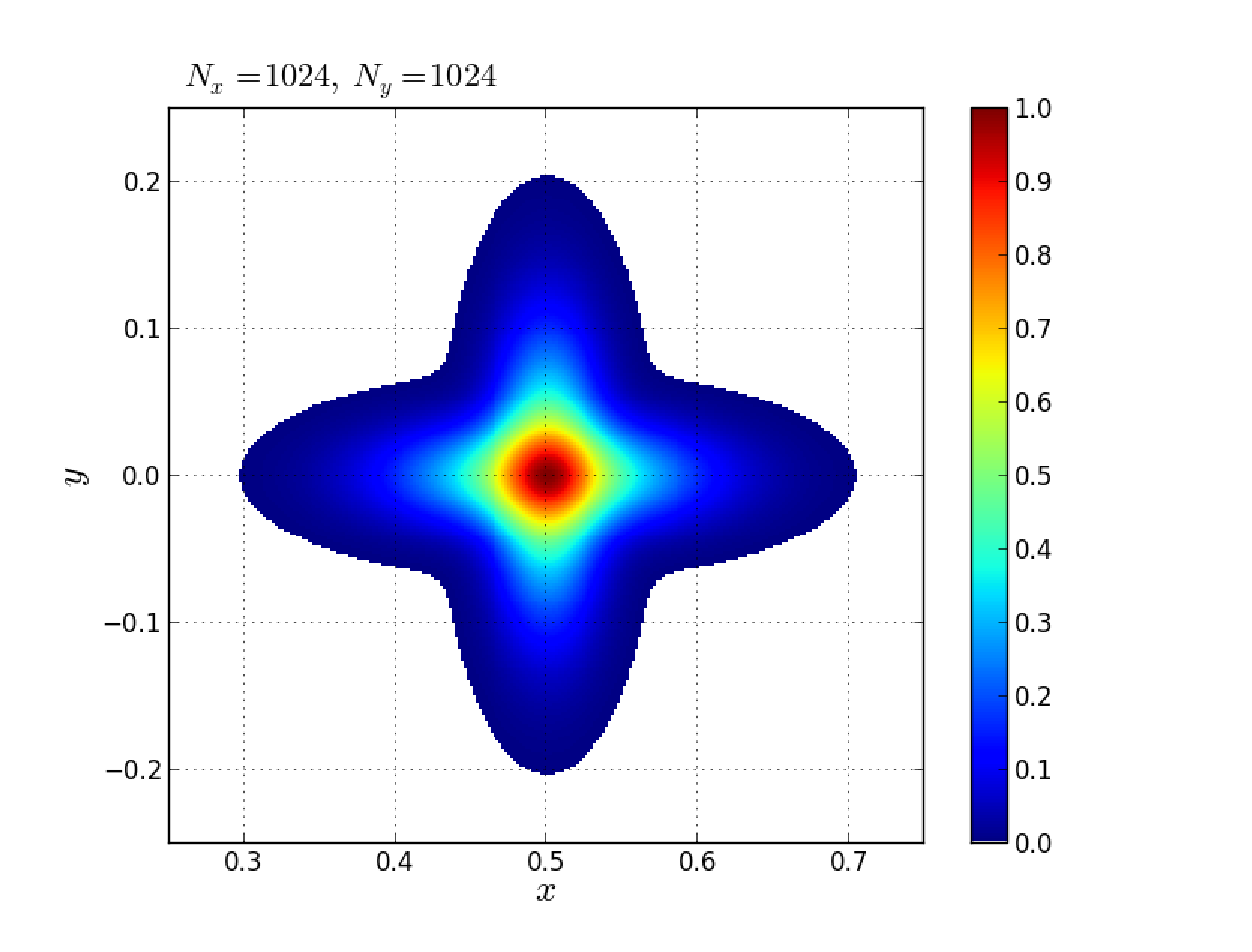
\includegraphics[width=0.75\hsize]{graphics/f0_2drot_exact_highres}
\captionsetup{width=0.65\hsize}\captionof{figure}{The cosine cross initial density $N_x = N_y = 1024$ spatial cells spanning $(x,y)$.}
\label{fig:f0_2drot}
\end{minipage}
}}
\end{table}

We defer the convergence analysis for future work, but report preliminary results using four splitting schemes where the names are kept identical to the seminal paper by Blanes et. al \cite{Blanes02}, which was also done by \cite{Guclu14}. Table \ref{tbl:splitting_coefficients} summarizes the splitting coefficients, which is reproduced from \cite{Blanes02} using the notation of section \ref{subsec:Operator_splitting_theory} for transport operators in space $\mathcal{X}^{c_i\tau} \coloneqq \exp(c_i\tau\Lambda_x)$ along the $x$ direction and $\mathcal{Y}^{d_i\tau} \coloneqq \exp(d_i\tau\Lambda_y)$ along the $y$ direction.  In the terminology of Blanes et. al, we consider two orderings for symmetric Runge-Kutta-Nystr\"{o}m (SRKN) compositions. These orderings are labeled as type $c$ and $d$ ($\text{SRKN}_s^c$ and $\text{SRKN}_s^d$, respectively) for as many substages $s$ as required. Here, the superscripting labels the outermost terms in the compositions, where $c$ labels coefficients corresponding to the fractional time steps taken of the full step $\tau$ by the first operator ($\mathcal{X}$) and $d$ plays the analogous role for the second ($\mathcal{Y}$).

The result quoted earlier for the $N$th order scheme \eqref{eq:nth_order_scheme_exp} from section \ref{subsec:Operator_splitting_theory} corresponded to the first ordering, which can be equivalently represented as:

\begin{equation}\text{SRKN}_s^c \coloneqq \mathcal{X}^{c_1\tau}\circ\mathcal{Y}^{d_1\tau}\circ \ldots \circ \mathcal{X}^{c_s\tau}\circ\mathcal{Y}^{d_s\tau}\mathcal{X}^{c_{s+1}\tau} \label{eq:SRKN_sc}
\end{equation}

\noindent where $c_{s+2-i} = c_i$ and $d_{s+1-i} = d_i$. These types of compositions contain schemes such as the second order accurate LF2 (leapfrog or Strang) method, and the fourth order Yoshida Y4 method. The second ordering is then given by

\begin{equation}\text{SRKN}_s^d \coloneqq \mathcal{Y}^{d_1\tau}\circ\mathcal{X}^{c_1\tau} \circ \ldots \circ \mathcal{Y}^{d_s\tau}\circ\mathcal{X}^{c_s\tau}\circ\mathcal{Y}^{d_{s+1}\tau} \label{eq:SRKN_sd}
\end{equation}

\noindent where $c_{s+1-i} = c_i$ and $d_{s+2-i} = d_i$. The two methods used in this work O6-4 and O11-6 follow this prescription.

\begin{table}
\ra{1.3}
\begin{tabular}{@{}lllllll@{}}\toprule[2 pt]
\phantom{a}$\mathcal{X}$ coefficients & $\mathcal{Y}$ coefficients &  $\mathcal{X}$ coefficients & $\mathcal{Y}$ coefficients & \\ \midrule
$\textbf{LF2}: \text{SRKN}_1^c, \,\, N = 2$ & & \textbf{O11-6}: $\text{SRKN}_{11}^d,\,\, N = 6$\\
 $c_1$ = 1/2 & $d_1$ = 1 &   $c_1 = 0.123229775946271 $ & $d_1 = 0.0414649985182624 $ &\\
$c_2$ = 1/2 &  &   $c_2 = 0.290553797799558 $ & $d_2 = 0.198128671918067  $ &\\
&&  $c_3 = -0.127049212625417$ & $d_3 = -0.0400061921041533 $ &\\
$\textbf{Y4}: \text{SRKN}_3^c,\,\, N = 4$ & & $c_4 = -0.246331761062075 $ & $d_4 = 0.0752539843015807 $ &\\
$c_1 =  \frac{1}{2(2 - 2^{1/3})}$ & $d_1 = \frac{1}{2 - 2^{1/3}}$ &  $c_5 = 0.357208872795928 $ & $d_5 = -0.0115113874206879$ &\\ 
$c_2 = \frac{1 - 2^{1/3}}{2(2 - 2^{1/3})}$   & $d_2 = -\frac{2^{1/3}}{2 - 2^{1/3}}$ & $c_6 = 1 - 2(c_1 + \ldots + c_5)$ & $d_6 = 1/2 - (d_1 + \ldots + d_5)$ &\\
$c_3 = c_2$   & $d_3 = d_1$ & \\
$c_4 = c_1$   &  \\
&&&\\
\textbf{O6-4}: $\text{SRKN}_6^d,\,\, N = 4$\\
$c_1 = 0.245298957184271$ & $d_1 = 0.0829844064174052 $ \\
$c_2 = 0.604872665711080$ & $d_2 = 0.396309801498368 $ \\
$c_3 = 1/2 - (c_1 + c_2)$ & $d_3 = -0.0390563049223486  $ \\
 & $d_4 = 1 - 2(d_1 + d_2 + d_3) $ \\
\bottomrule[2 pt]
\end{tabular}
\caption{Splitting coefficients are given for various schemes. Two $\text{SRKN}_s^c$ methods are listed (LF2 and Y4 \cite{Yoshida90}), as well as two optimized  $\text{SRKN}_s^d$ methods presented by Blanes et. al \cite{Blanes02} (O6-4 and O11-6). The order of accuracy $N$ is also recorded. }
\label{tbl:splitting_coefficients}
\end{table}

The various schemes were used to solve the 2D rotating advection system for the initial cosine cross distribution. An example of a set of plots produced by the LF2 scheme is given in the following series.

\begin{figure}[h!] 
\label{fig:var_vel} 
\captionsetup{width=0.48\linewidth}
\begin{minipage}[b]{0.5\linewidth}
\centering
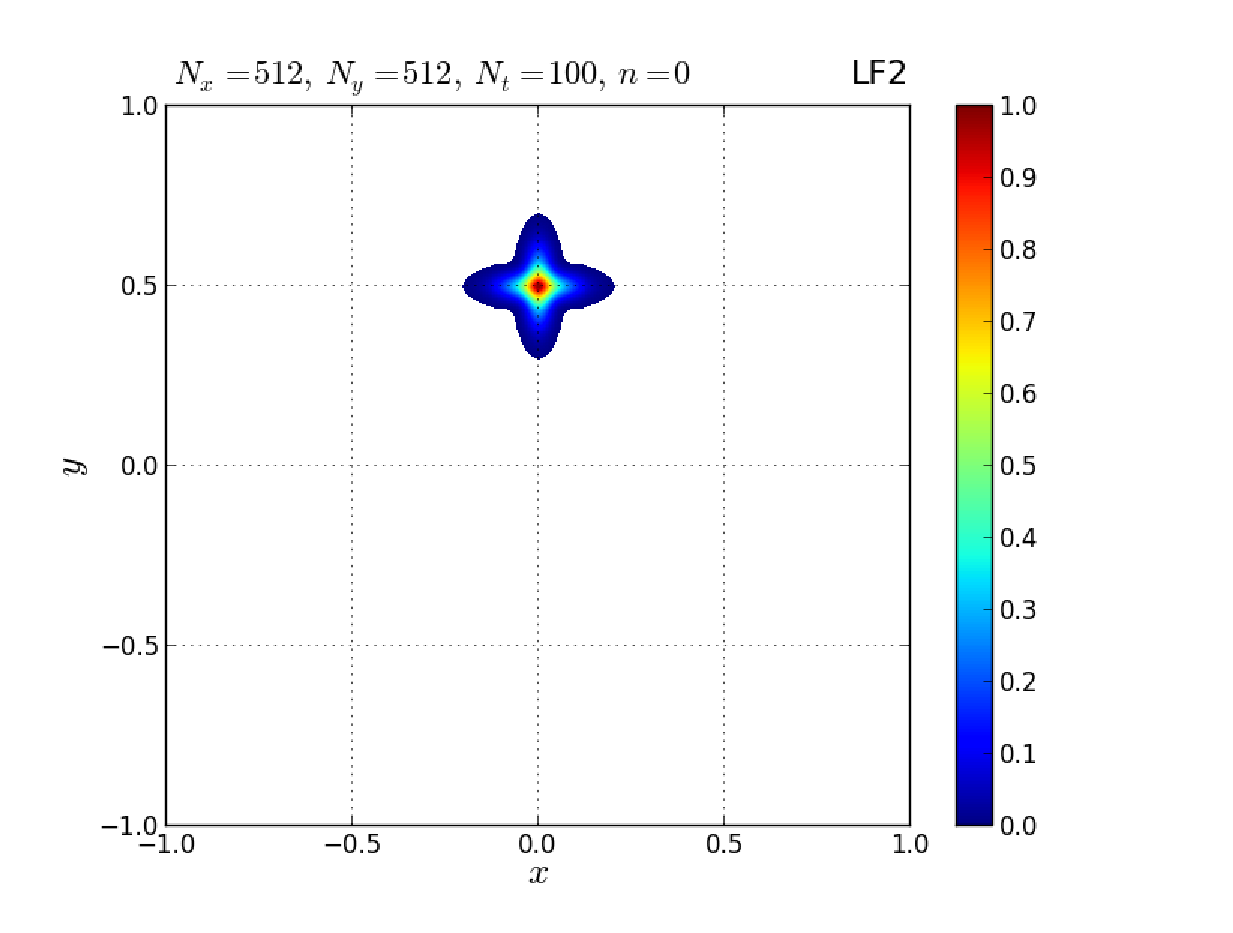
\includegraphics[width=\linewidth]{graphics/plot_-_flower_F12_Nx512Nt100_it00000_eps}
\caption{2D rotating case: time $t^0 = 0$}
\vspace{4ex}
\end{minipage}%%
\begin{minipage}[b]{0.5\linewidth}
\centering
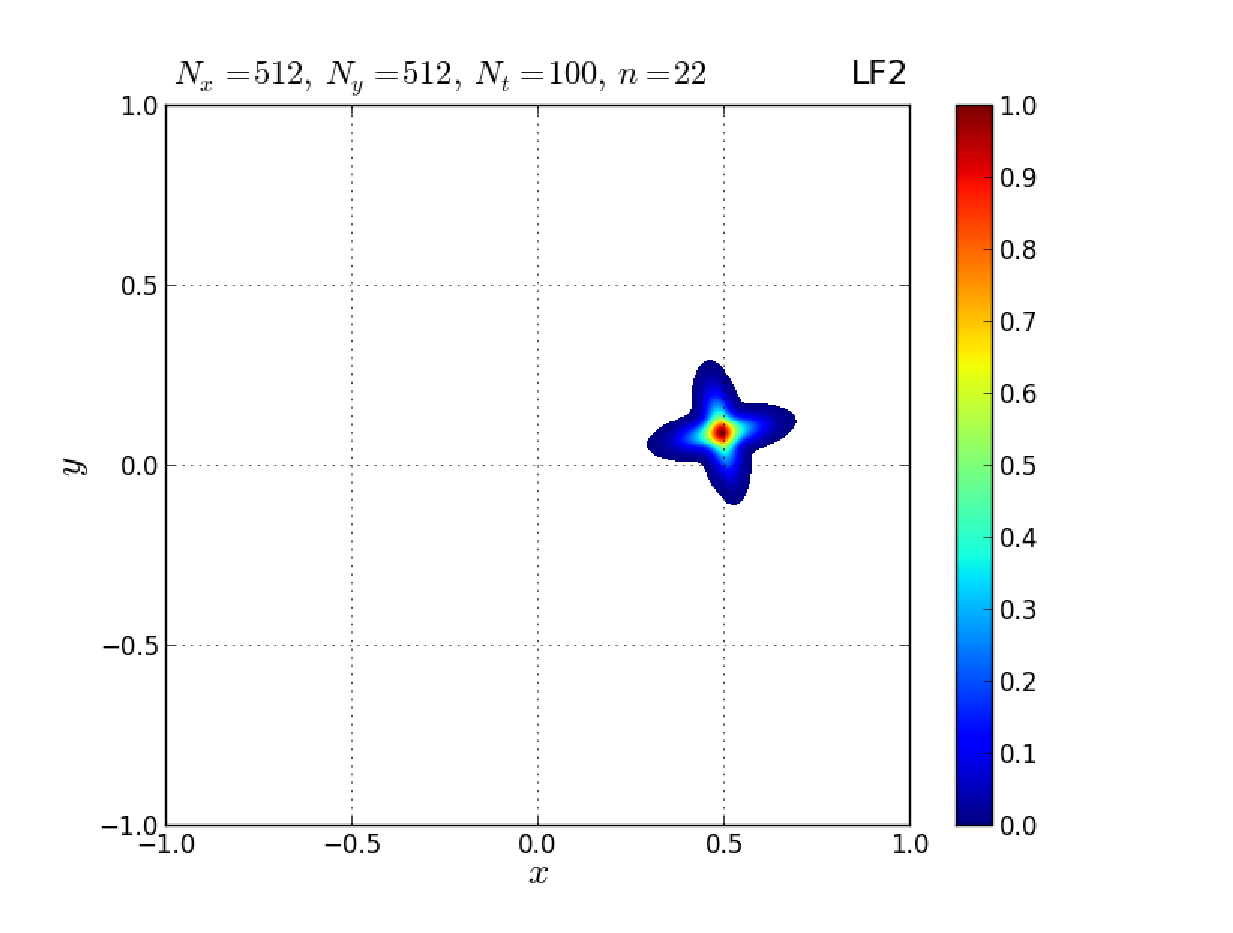
\includegraphics[width=\linewidth]{graphics/plot_-_flower_F12_Nx512Nt100_it00022_eps}
\caption{2D rotating case: time $t^{22} = 0.22$}
\vspace{4ex}
\end{minipage} 
\begin{minipage}[b]{0.5\linewidth}
\centering
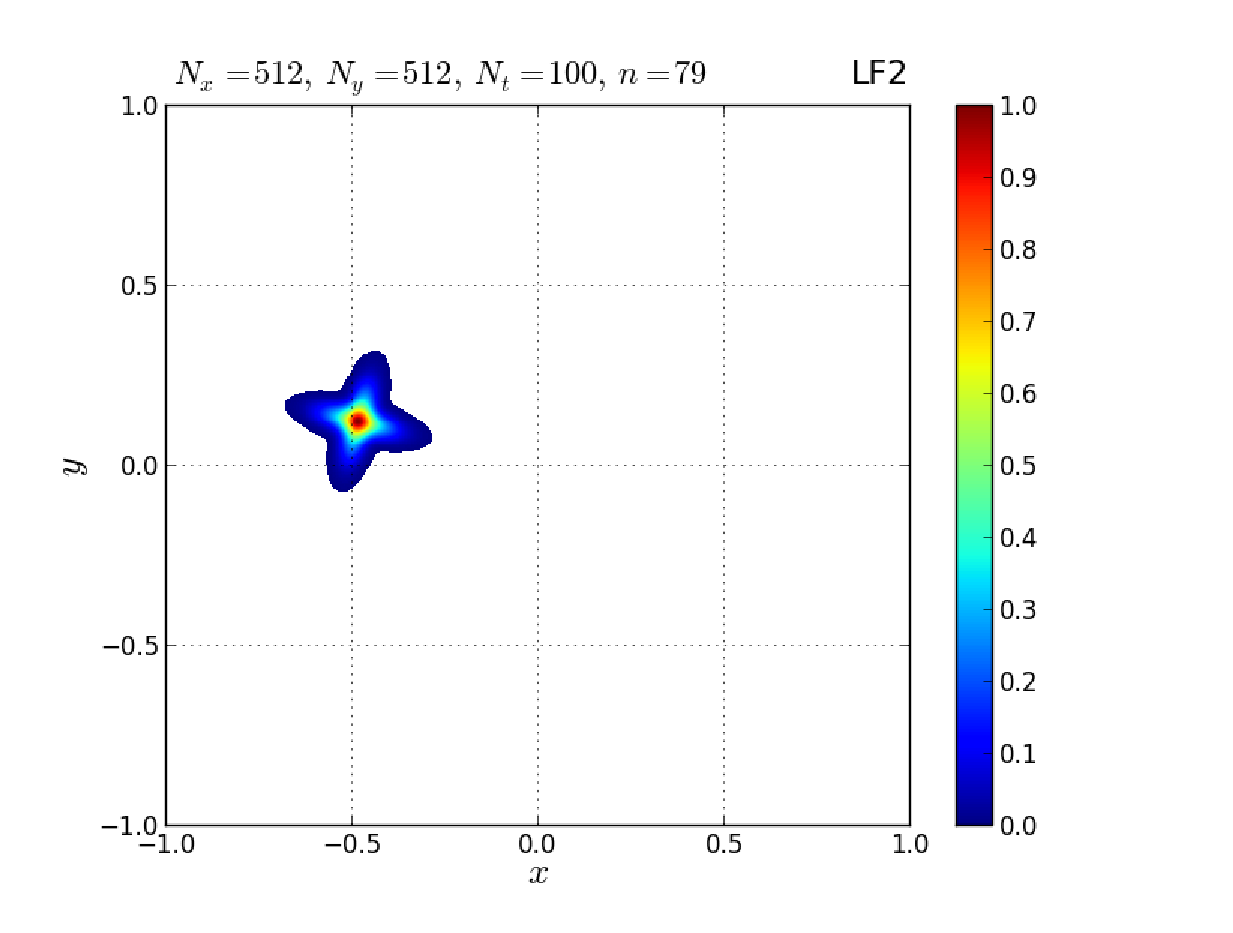
\includegraphics[width=\linewidth]{graphics/plot_-_flower_F12_Nx512Nt100_it00079_eps}
\caption{2D rotating case: time $t^{79} = 0.79$}
\vspace{4ex}
\end{minipage}%% 
\begin{minipage}[b]{0.5\linewidth}
\centering
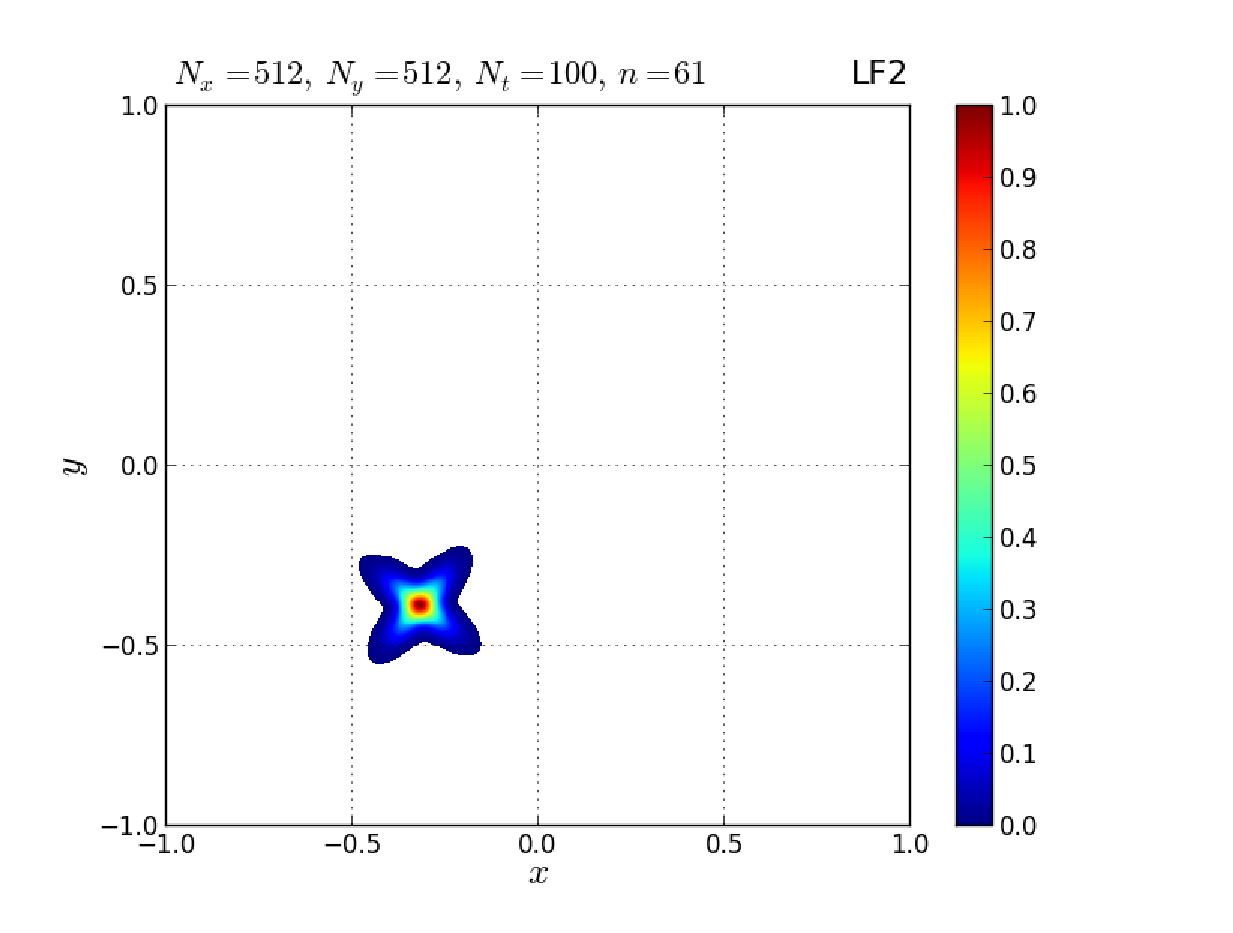
\includegraphics[width=\linewidth]{graphics/plot_-_flower_F12_Nx512Nt100_it00061}
\caption{2D rotating case: time $t^{54} = 0.61$}
\vspace{4ex}
\end{minipage} 
\end{figure}


To assess the error, we seek a relevant extension of the NRMSE error for the 1D case to obtain the global error. The straightforward generalization is the 2D measure of the averaged global error:

\begin{equation}\overline{\text{GE}}_{h} = \frac{1}{\sqrt{L_x L_y}}\left[\sum\limits_{i = 0}^{N_x - 1}\sum\limits_{k = 0}^{N_y - 1} [f_{_{\mathrm{CS}}}(T,x_i,y_k) - f_{_{\mathrm{exact}}}(T,x_i,y_k)]^2\Delta x\Delta y\right]^{1/2} \label{eq:GE_2D}\end{equation}

\noindent Here, $h$ is short for the finite grid space $h = (\Delta x, \Delta y)$. In other words, we elect to use a scaled Frobenius norm $||\cdot ||_F$, where the definitions for the domain lengths $(L_x,L_y)$ are spanned by $N_x$ and $N_y$ cells with spacings $\Delta x$ and $\Delta y$ in their respective directions. A time mesh refinement analogous to the spatial mesh refinement exercise performed earlier in this section for the 1D cases allows one to verify the theoretical order of convergence through successive simulations. Again, this exercise will be part of future work. The aim here is to only showcase the implementation of four popular split schemes, and to compare their global errors, which is summarized in table \ref{tbl:split_scheme_errors}. A plot of the error for the case of LF2 at the end of a full simulation is also given for comparison.



\begin{table}
\centering
\makebox[0pt][c]{\parbox{1.1\textwidth}{%
\begin{minipage}{0.59\hsize}
\centering
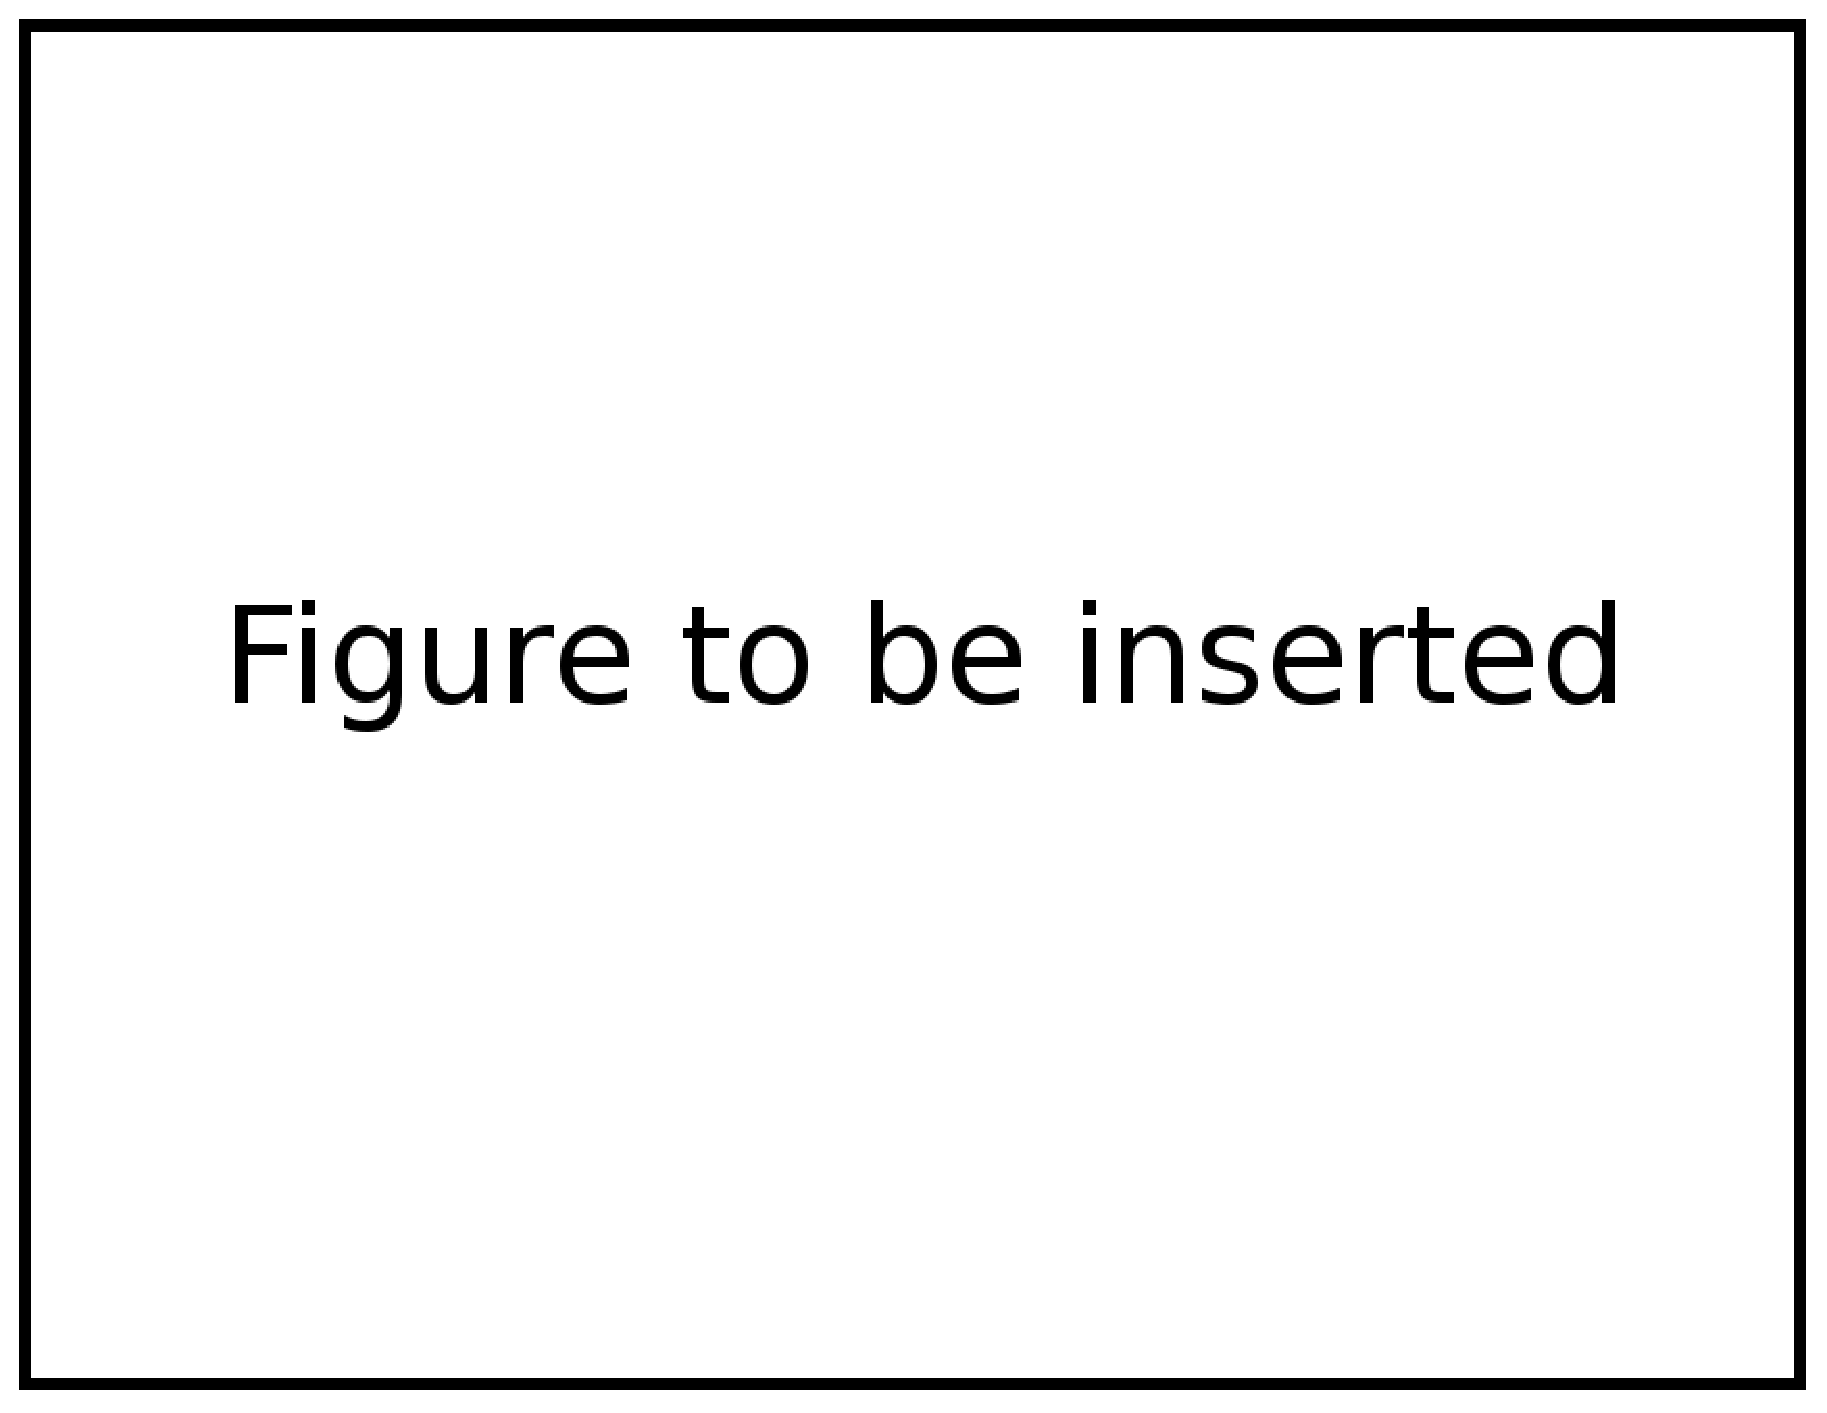
\includegraphics[width=0.5\hsize]{insertfigure}
\captionsetup{width=0.75\hsize}  \captionof{figure}{[PLACEHOLDER] for error plot at time t = T.}
 \label{fig:FD5_GB3_Nx128}
\end{minipage}
\begin{minipage}{0.45\hsize}
\centering
\ra{1.3}\captionsetup{width=7cm}
\begin{tabular}{@{}llll@{}}\toprule
& $\text{NRMS}(\text{GE}_{h})$ & Sim. time [s] \\ \midrule
$\phantom{a}$Scheme\\
$\phantom{a}LF2$ & $4.5338\times 10^{-3}$ & $5.2938\times 10^{3}$ \\
$\phantom{a}Y4$ & $1.4368\times 10^{-3}$ & $1.0561\times 10^{4}$ \\
$\phantom{a}O6$-4 & $2.1483\times 10^{-5}$ & $1.6298\times 10^{4}$ \\
$\phantom{a}O11$-6 & $3.9634\times 10^{-7}$ & $2.9528\times 10^{4}$ \\
\bottomrule
\end{tabular}
\captionof{table}{Error and simulation times required for various splitting schemes applied to the solution of \ref{eq:2Drot_advec_eq} for the initial density \eqref{eq:cosine_cross}. The normalized root mean square (NRMS) of the global error (GE$_h$) for the mesh $h = (\Delta x, \Delta y)$ is given by eq. \eqref{eq:GE_2D}. For all simulations, $N_x = N_y = 256$, $N_t = 25$.}
\label{tbl:split_scheme_errors}
\end{minipage}
}}
\end{table}


\subsection{1D-1V Vlasov-Poisson test case: external electric field}

\indent\indent With the split methods implemented, the intermediate test case between the one-dimensional scenario and the full two-dimensional phase space ($(x,v)$) calculation required for the Vlasov-Poisson system with self-consistent electric field calculations based on the charged particle positions is the reduced problem of a constant electric field in time (e.g. an externally applied $E$-field).





\chapter{Future work}\label{chap:Future_work}


\section{Boundaries}

[Motivate in brief that the boundaries invariably presents having to deal with discontinuities, e.g. in temperature distributions of electrons and ions]

\subsection{High order boundary treatment through defect correction methods}

[Intro to defect correction theory and how to apply to boundary]

%\subsection{2D tokamak boundary}
%\subsection{stellarator boundary}
\section{Collisions}

[models of collisions]

\subsection{High order collision treatment through Hartman filters}


[Intro to Hartman filters]

%\subsection{Lorentz collision models}
%\subsection{Self-consistent collision term calculation from Rosenbluth potentials}
%\subsection{Test case: Angular spreading of a beam distribution from Coulomb collisions}

%\section{The convected scheme in magnetized plasmas}
%\subsection{Boundaries and Chodura sheath tracking}
%\subsection{Transport in ergodic regions}

\chapter{Summary}

\indent\indent We have presented a preliminary framework demonstrating the design of arbitrarily high order accurate solutions to reduced cases of the Boltzmann-Maxwell system with the goal of moving forward to handle the Boltzmann-Poisson system. We propose as an immediate objective to work towards extending these high order accurate solutions to the Vlasov-Poisson system with self-consistent field calculations using the corrected convected scheme implemented in this document in tandem with high order splitting techniques (e.g. O11-6). As this is a well studied problem, there exist a number of benchmark cases that will allow for not only numerical verification and validation, but also to permit comparison with experiment. 

The next goal is to move towards developing a framework to handle boundaries and collisions (a Boltzmann equation) to high order accuracy. To this end, a Hartman filter will be looked into for handling the boundary properly, and the possibility of employing so-called deferred correction techniques will be investigated for collisions. The presence of the boundary will provide access to the interesting problem of sheath physics and the deterministic nature of the convected scheme kinetic solutions will allow appropriate tracking of the sheath thickness. On the other hand, the addition of collisions will allow us to investigate a more recent challenge in plasma physics collisional theory. That is, some studies suggest that large angle collisions are far more frequent than classically expected. Accurate modeling of collisions will provide the means to investigate this firsthand. Other researchers have observed the onset of beam-plasma instabilities in edge plasma show provisional dependence on neutral beam injection velocity. 

We aim to extend the number of dimensions in our model, beginning with velocity in order to capture more of the physics involved in the edge. If progress permits, we will work towards extending a second spatial dimension. Including an additional velocity component gives a scenario where the effect of collisions and magnetic fields can be explored so that utmost goal could be extending high order methods to the case of magnetized plasmas (Boltzmann-Maxwell systems). Adding the extra spatial dimension on top of velocity will allow for the interaction between electrostatics in the edge with the cross $B$-field transport to be studied. Alternatively, the kinetic model could be used to inform the design of accurate fluid models for 2D edge problems.

\newpage

%\chapter*{Miscellaneous notes}

%N.B. This section contains extra thoughts that will either find placement in the proper context section, or otherwise removed from a final version.


%[Notes to self: (1) divertors in tokamaks are accomplished with external coils creating nullclines in the B field (X-point), whereas in stellarators (e.g. W7-X) the intrinsic island formation naturally diverts power effluxes to zones where divertor plates can be installed. In this way, it is often said that stellarators possess a ``natural,'' \emph{island} divertor. (2) insert comment somewhere about steady-state vs. pulsed operations in stellarators vs. tokamaks. It is modestly encouraging in tokamaks that a large fraction of sustained current can be generated by the accompanied bootstrap current; however, a tokamak in steady-state operation has not been demonstrated insofar (nor has it been seen to be a necessary pathway provided pulsed operation can be accomplished with sufficiently high frequencies)].


%\emph{Convected scheme} (CS), a forward-trajectory semi-Lagrangian method, will be extended from an established baseline application for constant advection equations to the collisional Boltzmann transport equation. In natural steps, we aim to proceed from the preliminary work presented here (constant advection equation solutions) to include more of the physics of the full kinetic equation.


% and http://www.iop.org/Jet/fulltext/JETP93082.pdf ].

%\indent Computational models are aptly designed exclusively for either the core \emph{or} the edge. A significant motivator for this segmentation is the starkness of difference in scales between the two regions. Further, both regions lend themselves towards distinct choices for what would be considered more natural coordinates given the differences in magnetic topology. The core and edge may also be operating in different regimes (fluid vs. kinetic). By partitioning codes a particular experiendency is inherited by pursuing codes that operate with magnetic or flux coordinates for the core region. A common practice in such codes is to assume the existence of nested magnetic flux surfaces. This comes at the cost of being unable to straightforwardly couple codes to an edge code, whose field lines are by definition open. A further convenience in core codes such as GENE engage the idea that the distribution function can be linearly superposed as an averaged Maxwellian and a fluctuating component. Such a formulation would be not valid in the nonlinear, nonlocal thermodynamic equilibrium region of the edge; the full plasma kinetic equation must be solved nonlinearly (so-called \emph{full-f}) solutions. In the edge, modeling the distribution function as deviations from an equilibrium Maxwellian is not always permissible.

%\indent While a large portion of fusion research is dedicated towards the hot plasma core where fusion occurs, it is evident as Stangeby frames it, that contrary to what might have been hoped for the edge ``will not take care of itself,'' but instead must be directly addressed. In this way, substantial interest has been garnered for looking at this $\sim$ cm region of the plasma volume. The phenomena that shows

%\indent Codes:


%\begin{enumerate}
%\item SolEdge2D
%\item SOLPS
%\item EDGE2D-EIRENE
%\item UEDGE (US)
%\item SONIC (JP)
%\end{enumerate}

%\indent Issues with codes

%\begin{enumerate}
%\item statistical noise (MC), especially in sparse regions of phase space
%\item run time diverges with machine size (SOLPS: ~ 3 months for ITER simulation, DEMO ~ 1 year \cite{seminaire_paris})
%\item in semi-detached situations the kinetic equation becomes numerically stiff $\Rightarrow$ need to resolve a wide separation of scales
%\end{enumerate}


%\subsection{Indirect Drive}
%As with direct drive, the use of lasers is a main component of indirect drive but instead of directly impinging on the target surface, in this scenario a high Z material, typically gold, lead or depleted uranium, is illuminated by the lasers. The high Z material is formed into a cylinder called a ``hohlraum'' with holes in the caps to allow the lasers to enter and irradiate the inner surface of the hohlraum. This is done to smooth the radiation incident onto the target as the laser irradiation of the hohlraum surface leads to the production of an x-ray spectrum that uniformly impinges on the target capsule. This procedure smooths out any laser irregularities in the individual lasers but comes with additional loss mechanisms due to stimulated Raman scattering, cross beam interactions as the lasers enter the hohlraum, backscatter of laser light through the laser entrance holes and radiation losses through the hohlraum wall \cite{nif-indirect}.


%\chapter{Proposed Research}
%Going forward, the addition of the lead equation of state and opacity data using BADGER and YAC\cite{yuan} is a logical first step to upgrade the simulations. Adding this functionality into the simulations will be useful when moving towards a more realistic target geometry as represented in the figure from the cooper simulation \ref{cooper}. As with the cooper simulation, adding the energy to a compressed DT fuel material and allowing that material and energy to spread outwards through a hohlraum and into the target chamber will be a much more accurate simulation of the chamber dynamics. Additionally, working closely with the FLASH Computational Center at the University of Chicago to add multi-group radiation physics into the code is an important step in making the code more realistic. Adding the above features and running to a longer time will extend the simulation from its current status to one that more closely resembles a stationary expanding target in the reactor chamber.\\
%\indent While studying a stationary target is a logical starting point from which to build from, the velocity of the target from injection cannot be ignored. The 75 ms repetition rate for power production requires a 200 $ m/s $ target velocity and this factor has not been taken into consideration in any past published simulations of the reactor chamber. The effect this velocity will have on the disassembly of the target, subsequent instability growth, material mixing and either the dispersion or persistence of the mixed volume will be studied.\\
%\indent Another set of features that will be studied is the influence of initial perturbations on the hohlraum on target disassembly, instability growth and material mixing. As instabilities require an initial perturbation from which to grow and the current seeds come from numerical effects, the imposition of initial perturbations will provide a more controlled fashion to study instabilities. These instabilities and material mixing could be taken advantage of through changes to the design features of the reactor chamber, which also need to be studied in detail.
%There are a few main areas of future work to be concerned with moving forward. The first is to change the EoS and opacity data used in the FLASH simulations from the xenon surrogate for the target material to actual lead data produced from BADGER and YAC \cite{yuan}  This will allow for a more realistic simulation of the target expansion as data for a solid material will be used instead of a gas surrogate. This leads to the ability to then run the simulation to longer times in order to investigate mix of the target material with that of the gas. This information is critical to developing a feasible reactor as it will need to be taken into consideration if, after each shot there is a diffuse, vaporized lead material left in the chamber or if the material will expand and then re-condense into a more solid bunch. This will be seen by investigating the mix and the development of instabilities as the hohlraum material expands into the chamber.\\
%\indent Target injection into the chamber will also be explored by adding a wind term into the simulations. As the proposed reactor chamber requires a target explosion every 75 ms, the hohlraums will be injected with a speed of 200 $ cm/s $. This large velocity will undoubtedly have an effect on the growth of the instabilities and the target expansion in general and requires at least a two dimensional code to fully investigate. This will give an idea as to the interplay between the moving target and stagnant chamber gas as the target expands outward yet maintains forward motion due to conservation of momentum.\\
%\indent As instability growth and mix are the main avenue of investigation heading forward hohlraum designs that possibly promote mix and instability growth will also be considered. As explained in chapter \ref{cha-2d}, the later time Rayleigh-Taylor instabilities arise due to the seeding from the Kelvin-Helmholtz instabilities at short time and the numerical variations caused by the rezoning of the problem as the resolution is dropped to preserve runtime. By seeding the instabilities from the start, a more thorough investigation of the instability development can be preformed and the effects studied. Additionally, other properties of the effect on the target besides instability growth and mix can be studied.


\cleardoublepage


\nocite{*}

\bibliography{test}
\bibliographystyle{acm}

%\bibliographystyle{acm}













\end{document}
